% arara: pdflatex
% arara: makeindex: {style: latexindent.ist}
% arara: bibtex
% arara: pdflatex if changed (toFile('latexindent.aux')) || changed (toFile('latexindent.ind')) 
% arara: pdflatex if changed (toFile('latexindent.aux')) 
% arara: pdflatex if changed (toFile('latexindent.aux')) 
\documentclass[10pt]{article}
%   This program is free software: you can redistribute it and/or modify
%   it under the terms of the GNU General Public License as published by
%   the Free Software Foundation, either version 3 of the License, or
%   (at your option) any later version.
%
%   This program is distributed in the hope that it will be useful,
%   but WITHOUT ANY WARRANTY; without even the implied warranty of
%   MERCHANTABILITY or FITNESS FOR A PARTICULAR PURPOSE. See the
%   GNU General Public License for more details.
%
%   See <http://www.gnu.org/licenses/>.
\usepackage[left=4.5cm,right=2.5cm,showframe=false,
 top=2cm,bottom=1.5cm,marginparsep=2cm]{geometry} % page setup
\usepackage{lmodern}
\usepackage{parskip}                                 % paragraph skips
\usepackage{booktabs}                                % beautiful tables
\usepackage{listings}                                % nice verbatim environments
\usepackage{titlesec}                                % customize headings
\usepackage{titletoc}                                % customize headings
\usepackage{multicol}
\usepackage{changepage}                              % adjust width of page
\usepackage{fancyhdr}                                % headers & footers
\usepackage{fontawesome}
\usepackage[sc,format=hang,font=small]{caption}      % captions
\usepackage[backend=bibtex,sorting=ynt]{biblatex}    % bibliography
\usepackage{tcolorbox}                               % framed environments
\usepackage{tikz}
\usepackage{xparse}
\usepackage[charter]{mathdesign}                     % changes font
\usepackage[expansion=false,kerning=true]{microtype} % better kerning
\usepackage{enumitem}                                % custom lists
\usepackage{longtable}
\usepackage{array}
\usepackage{totalcount}
\usepackage{standalone}
% setup gitinfo2, as in the manual, details just above begin{document}
\usepackage[mark]{gitinfo2}
% tikz, tcolorbox libraries
\usetikzlibrary{positioning}
\usetikzlibrary{decorations.pathmorphing}
\usetikzlibrary{decorations,shapes}
\usepackage{varioref}                                % the documentation library from tcolorbox loads hyperref
\tcbuselibrary{breakable,xparse,documentation,hooks,raster}
\hypersetup{
 pdfauthor={Chris Hughes},
 pdftitle={latexindent.pl package},
 pdfkeywords={perl;beautify;indentation},
 bookmarksnumbered,
 bookmarksopen,
 linktocpage,
 colorlinks=true,
 linkcolor=blue,
 citecolor=black,
}
\usepackage{cleveref}

% create my own star style, for re-use at various points
\tikzset{cmhstar/.style={star,star point ratio=2.25,fill=cmhgold,draw=orange,}}

% shortcut command for displaying star in documentation
\newcommand{\stardemo}[1][]{\begin{tikzpicture}
 \node at (10:.1cm)[very thin,cmhstar,scale=0.25,rotate=20,#1]{};
 \node at (120:.1cm)[very thin,cmhstar,scale=0.15,rotate=-10,#1]{};
 \node at (235:.1cm)[very thin,cmhstar,scale=0.2,rotate=-20,#1]{};
 \end{tikzpicture}}

% totalcount
\DeclareTotalCounter{lstlisting}

% customise the \tcbdocnew command
\tcbset{doclang/new={{\bfseries\color{green!50!black}N\normalfont\color{black}}}}
\tcbset{doclang/updated={{\bfseries\color{green!50!black}U\normalfont\color{black}}}}
\tcbset{doc marginnote={width=1.6cm}}

% \announce * { YYYY-MM-DD }*{ <announcement text> }
%
%   NEW as of current version
%       \announce*{date}*[text] means *updated* as of <date>
%       \announce*{date}[text]  means *new* as of <date>
%
%   NOT new as of current version
%       \announce{date}*[text] means *updated* as of <date>
%       \announce{date}[text]  means *new* as of <date>
%
\NewDocumentCommand{\announce}{ s m s m }{%
 \IfBooleanTF{#1}%
 {% \announce*
  % NEW in current version
  \tcbdocmarginnote[colframe=orange,
   overlay={\node at ([yshift=0mm,xshift=1mm]frame.north east) {\stardemo}; }]{%
   \IfBooleanTF{#3}%
   {% \announce*{date}*[text] means *updated* as of <date>
    \tcbdocupdated{#2}%
   }%
   {% \announce*{date}[text] means *new* as of <date>
    \tcbdocnew{#2}%
   }%
  }%
  \IfBooleanTF{#3}%
  {%
   \addcontentsline{new}{cmhtitle}{#4 (U)}%
  }%
  {%
   \addcontentsline{new}{cmhtitle}{#4 (N)}%
  }%
 }%
 {% \announce
  % NOT new in current version
  \tcbdocmarginnote[colframe=gray!50!white,
   doclang/new={{\color{gray}N\normalfont\color{gray}}},
   doclang/updated={{\color{gray}U\normalfont\color{gray}}},
  ]{%
   \IfBooleanTF{#3}%
   {% \announce{date}*[text] means *updated* as of <date>
    \tcbdocupdated{#2}%
   }%
   {% \announce{date}[text] means *new* as of <date>
    \tcbdocnew{#2}%
   }%
  }%
 }}

\reversemarginpar
% bibliographies
\addbibresource{latex-indent}
\addbibresource{contributors}

% http://tex.stackexchange.com/questions/122135/how-to-add-a-png-icon-on-the-right-side-of-a-tcolorbox-title
\newtcolorbox{warning}{parbox=false,
 breakable,
 enhanced,
 arc=0mm,
 colback=red!5,
 colframe=red,
 leftrule=12mm,%
 title={Warning!},
 overlay={\node[anchor=north west,outer sep=2pt] at (frame.north west) {
\includegraphics[width=8mm]{warning}}; }
}

\definecolor{harvestgold}{cmyk}{0.00, 0.05, 0.51, 0.07}  %EDE275
\definecolor{cmhgold}{cmyk}{0,0.178,0.909,0.008}         %FDD017
\colorlet{cmhgray}{gray!30!white}

\makeatletter
\tcbset{
 addtolol/.style={list entry={\kvtcb@title},add to list={lol}{lstlisting}},
 addtololstar/.style={list entry={\kvtcb@title},add to list={lol}{lstlistingstar}},
 cmhlistings/.style={
   colback=blue!5!white,
   colframe=white!25!black,colback=white,
   top=0cm,
   bottom=0cm,
   left=0mm,
   listing only,
   center title,
   listing engine=listings,
   listing options={showtabs=true,tabsize=4,showspaces=true},
   boxrule=0pt,
   toprule=1pt,bottomrule=1pt,
   titlerule=1pt,
   colframe=white!40!black,
   colback=white,
   sharp corners,
   colbacktitle=white!75!black
  },
 tex-TCB/.style={
   listing only,
   listing engine=listings,
   left=0cm,
   boxrule=0pt,
   sharp corners,
   center title,
   colframe=white!40!black,
   colback=white,
   sharp corners,
   colbacktitle=white!75!black,
   toprule=1pt,
   bottomrule=1pt,
   titlerule=1pt,
  },
 yaml-TCB/.style={
   listing only,
   listing engine=listings,
   left=0cm,
   boxrule=0pt,
   sharp corners,
   center title,
   colbacktitle=white!75!blue,
   colframe=white!25!blue,
   colback=white!90!blue,
   toprule=2pt,
   titlerule=2pt,
  },
 MLB-TCB/.style={
   yaml-TCB,
   center title,
   colframe=cmhgold,
   colbacktitle=harvestgold,
   colback=white!60!cmhgold,
   width=0.9\linewidth,
   before=\centering,
   enhanced,
   overlay={\node[anchor=north east,outer sep=2pt,draw=cmhgold,very thick,double,fill=harvestgold,font =\small] at ([yshift=-3mm]frame.north east) {\texttt{-m}}; }
  },
 replace-TCB/.style={
   yaml-TCB,
   center title,
   colbacktitle=white!75!green,
   colframe=white!25!green,
   colback=white!90!green,
   width=0.9\linewidth,
   before=\centering,
   enhanced,
   overlay={\node[anchor=north east,outer sep=2pt,draw=white!25!green,very thick,circle,fill=white!75!green,font =\small] at ([yshift=-3mm]frame.north east) {\texttt{-r}}; }
  },
 yaml-obsolete/.style={
   listing only,
   listing engine=listings,
   left=0cm,
   boxrule=0pt,
   sharp corners,
   center title,
   toprule=2pt,
   titlerule=2pt,
   colframe=white!25!red,
   colbacktitle=white!75!red,
   colback=white!90!red,
  },
 new-to-this-version/.style={
   enhanced,
   overlay app={\node at ([yshift=0mm,xshift=0mm]frame.north east) {\stardemo[scale=1.2]}; },
   addtololstar,
  },
}

\DeclareTCBListing[use counter=lstlisting]{cmhlistings}{s O{} m m}{%
 cmhlistings,
 IfBooleanTF={#1}{new-to-this-version}{addtolol},
 center title,
 title={\color{black}{\scshape Listing \thetcbcounter}: ~#3},label={#4},
 listing engine=listings,
 listing options={#2},
}

\DeclareDocumentEnvironment{cmhtcbraster}{O{}}{\begin{tcbraster}[
  new-to-this-version/.style={
    enhanced,
    overlay app={\node[anchor=south east] at ([yshift=-3mm,xshift=3mm]frame.north east) {\stardemo[scale=1.2]}; },
    addtololstar,
   },
  raster valign=top,raster columns=2,#1]}{\end{tcbraster}}

% \cmhlistingsfromfile
%                   * no star: not new, star: new   #1
%                   [ listing options ]             #2
%                   {<name of listing file>}        #3
%                   [<options for tcolorbox>]       #4
%                   {<title>}                       #5
%                   {<label>}                       #6
%
% for example,
%   \cmhlistingsfromfile*[listing options]... is NEW
%   \cmhlistingsfromfile[listing options]...  is not new
\DeclareTCBInputListing[use counter=lstlisting]{\cmhlistingsfromfile}{s O{} m O{} m m}{%
 cmhlistings,
 listing file={#3},
 listing options={style=tcblatex,showspaces=false,#2},
 title={\color{black}{\scshape Listing \thetcbcounter}: ~#5},label={#6},
 #4,
 IfBooleanTF={#1}{new-to-this-version}{addtolol},
}

\makeatletter
\@tempswafalse
\def\@tempa{draft}
\@for\next:=\@classoptionslist\do
{\ifx\next\@tempa\@tempswatrue\fi}
\if@tempswa % draft option is active
 \RenewDocumentCommand{\cmhlistingsfromfile}{s O{} s m O{} m m}{\captionof{lstlisting}{#6}\label{#7}}
 \renewcommand{\stardemo}[1][]{$\star$}
\fi

% command shell
\newtcblisting{commandshell}{colback=black,colupper=white,colframe=yellow!75!black,
 listing only,listing options={style=tcblatex,language=sh,
   morekeywords={latexindent,pl},
   keywordstyle=\color{blue!35!white}\bfseries,
  },
 listing engine=listings,
 left=0cm,
 every listing line={\textcolor{red}{\small\ttfamily\fontseries{b}\selectfont cmh:$\sim$\$ }}}

% dosprompt
\newtcblisting{dosprompt}{
 colback=black,
 colupper=white,
 colframe=yellow!75!black,
 listing only,
 listing options={
   language=command.com,
   morekeywords={latexindent,pl},
   keywordstyle=\color{blue!35!white}\bfseries,
   basicstyle=\small\color{white}\ttfamily
  },
 listing engine=listings,
 left=0cm,
 every listing line={\textcolor{white}{\small\ttfamily\fontseries{b}\selectfont C:\textbackslash Users\textbackslash cmh$>$}}}

\lstset{%
 basicstyle=\small\ttfamily,language={[LaTeX]TeX},
 numberstyle=\ttfamily%\small,
 breaklines=true,
 keywordstyle=\color{blue},                    % keywords
 commentstyle=\color{purple},    % comments
 tabsize=3,
}%
\DeclareTCBListing[use counter=lstlisting]{yaml}{O{} m O{} m}{
 yaml-TCB,
 listing options={
   style=tcblatex,
   numbers=none,
   numberstyle=\color{red},
   #1,
  },
 title={\color{black}{\scshape Listing \thetcbcounter}: ~#2},label={#4},
 #3,
}

\lstdefinestyle{yaml-LST}{
 style=tcblatex,
 numbers=none,
 numberstyle=\color{red},
}

\lstdefinestyle{demo}{
 numbers=none,
 linewidth=1.25\textwidth,
 columns=fullflexible,
}

\lstdefinestyle{lineNumbersTeX}{
 numbers=left,
 numberstyle=\color{blue},
}

\lstdefinestyle{fileExtensionPreference}{
 style=yaml-LST,
 firstnumber=44,linerange={44-48},
 numbers=left,
}

\lstdefinestyle{logFilePreferences}{
 style=yaml-LST,
 firstnumber=88,linerange={88-102},
 numbers=left,
}

\lstdefinestyle{verbatimEnvironments}{
 style=yaml-LST,
 firstnumber=106,linerange={106-109},
 numbers=left,
}

\lstdefinestyle{verbatimCommands}{
 style=yaml-LST,
 firstnumber=112,linerange={112-114},
 numbers=left,
}

\lstdefinestyle{noIndentBlock}{
 style=yaml-LST,
 firstnumber=119,linerange={119-121},
 numbers=left,
}

\lstdefinestyle{removeTrailingWhitespace}{
 style=yaml-LST,
 firstnumber=150,linerange={150-152},
 numbers=left,
}

\lstdefinestyle{fileContentsEnvironments}{
 style=yaml-LST,
 firstnumber=125,linerange={125-127},
 numbers=left,
}

\lstdefinestyle{lookForPreamble}{
 style=yaml-LST,
 firstnumber=133,linerange={133-137},
 numbers=left,
}

\lstdefinestyle{lookForAlignDelims}{
 style=yaml-LST,
 firstnumber=155,linerange={155-171},
 numbers=left,
}

\lstdefinestyle{indentAfterItems}{
 style=yaml-LST,
 firstnumber=233,linerange={233-240},
 numbers=left,
}

\lstdefinestyle{itemNames}{
 style=yaml-LST,
 firstnumber=246,linerange={246-248},
 numbers=left,
}

\lstdefinestyle{specialBeginEnd}{
 style=yaml-LST,
 firstnumber=252,linerange={252-265},
 numbers=left,
}

\lstdefinestyle{indentAfterHeadings}{
 style=yaml-LST,
 firstnumber=275,linerange={275-284},
 numbers=left,
}

\lstdefinestyle{noAdditionalIndentGlobalEnv}{
 style=yaml-LST,
 firstnumber=333,linerange={333-334},
 numbers=left,
}

\lstdefinestyle{noAdditionalIndentGlobal}{
 style=yaml-LST,
 firstnumber=333,linerange={333-345},
 numbers=left,
}

\lstdefinestyle{indentRulesGlobalEnv}{
 style=yaml-LST,
 firstnumber=349,linerange={349-350},
 numbers=left,
}

\lstdefinestyle{indentRulesGlobal}{
 style=yaml-LST,
 firstnumber=349,linerange={349-361},
 numbers=left,
}

\lstdefinestyle{commandCodeBlocks}{
 style=yaml-LST,
 firstnumber=364,linerange={364-379},
 numbers=left,
}

\lstdefinestyle{modifylinebreaks}{
 style=yaml-LST,
 firstnumber=494,linerange={494-496},
 numbers=left,
}

\lstdefinestyle{textWrapOptions}{
 style=yaml-LST,
 firstnumber=522,linerange={522-523},
 numbers=left,
}

\lstdefinestyle{textWrapOptionsAll}{
 style=yaml-LST,
 firstnumber=522,linerange={522-545},
 numbers=left,
}

\lstdefinestyle{oneSentencePerLine}{
 style=yaml-LST,
 firstnumber=497,linerange={497-521},
 numbers=left,
}

\lstdefinestyle{sentencesFollow}{
 style=yaml-LST,
 firstnumber=503,linerange={503-511},
 numbers=left,
}

\lstdefinestyle{sentencesBeginWith}{
 style=yaml-LST,
 firstnumber=512,linerange={512-515},
 numbers=left,
}

\lstdefinestyle{sentencesEndWith}{
 style=yaml-LST,
 firstnumber=516,linerange={516-521},
 numbers=left,
}

\lstdefinestyle{modifylinebreaksEnv}{
 style=yaml-LST,
 firstnumber=547,linerange={547-556},
 numbers=left,
}

\lstdefinestyle{replacements}{
 style=yaml-LST,
 firstnumber=608,linerange={608-616},
 numbers=left,
}

\lstdefinestyle{fineTuning}{
 style=yaml-LST,
 firstnumber=619,linerange={619-671},
 numbers=left,
}

% stars around contributors
\pgfdeclaredecoration{stars}{initial}{
 \state{initial}[width=15pt]
 {
  \pgfmathparse{round(rnd*100)}
  \pgfsetfillcolor{yellow!\pgfmathresult!orange}
  \pgfsetstrokecolor{yellow!\pgfmathresult!red}
  \pgfnode{star}{center}{}{}{\pgfusepath{stroke,fill}}
 }
 \state{final}
 {
  \pgfpathmoveto{\pgfpointdecoratedpathlast}
 }
}

\newtcolorbox{stars}{%
 enhanced jigsaw,
 breakable, % allow page breaks
 left=0cm,
 top=0cm,
 before skip=0.2cm,
 boxsep=0cm,
 frame style={draw=none,fill=none}, % hide the default frame
 colback=white,
 overlay={
   \draw[inner sep=0,minimum size=rnd*15pt+2pt]
   decorate[decoration={stars,segment length=2cm}] {
     decorate[decoration={zigzag,segment length=2cm,amplitude=0.3cm}] {
       ([xshift=-.5cm,yshift=0.1cm]frame.south west) -- ([xshift=-.5cm,yshift=0.4cm]frame.north west)
      }};
   \draw[inner sep=0,minimum size=rnd*15pt+2pt]
   decorate[decoration={stars,segment length=2cm}] {
     decorate[decoration={zigzag,segment length=2cm,amplitude=0.3cm}] {
       ([xshift=.75cm,yshift=0.1cm]frame.south east) -- ([xshift=.75cm,yshift=0.6cm]frame.north east)
      }};
   \node[anchor=north west,outer sep=2pt,opacity=0.25] at ([xshift=-4.25cm]frame.north west) {\resizebox{3cm}{!}{\faGithub}};
  },
 % paragraph skips obeyed within tcolorbox
 parbox=false,
}

\newtcolorbox[auto counter]{example}{breakable,
 enhanced jigsaw,
 before skip=6pt,after skip=6pt,
 frame hidden,
 title={\llap{Example~\thetcbcounter\hspace{3mm}}},
 fonttitle=\bfseries,
 coltitle=black,
 attach title to upper,
 grow to left by=5mm,
 top=3mm,
 overlay unbroken={%
   \draw[thick,cmhgray] ([xshift=3mm]interior.north east)--([xshift=3mm]interior.south east);
   \path [fill=cmhgray] ([xshift=3mm]interior.north east) circle (.5mm);
   \path [fill=cmhgray] ([xshift=3mm]interior.south east) circle (1mm);
  },
 overlay first={%
   \draw[thick,cmhgray] ([xshift=3mm]interior.north east)--([xshift=3mm]interior.south east);
   \path [fill=cmhgray] ([xshift=3mm]interior.north east) circle (.5mm);
   %\path [draw=cmhgray,fill=white] ([xshift=3mm]interior.south east) circle (.5mm);
  },
 overlay last={%
   \draw[thick,cmhgray] ([xshift=3mm]interior.north east)--([xshift=3mm]interior.south east);
   %\path [fill=white,draw=cmhgray] ([xshift=3mm]interior.north east) circle (.5mm);
   \path [fill=cmhgray] ([xshift=3mm]interior.south east) circle (1mm);
  },
 parbox=false,
}

% copied from /usr/local/texlive/2013/texmf-dist/tex/latex/biblatex/bbx/numeric.bbx
% the only modification is the \stars and \endstars
\defbibenvironment{specialbib}
{\stars\list
 {\printtext[labelnumberwidth]{%
   \printfield{prefixnumber}%
   \printfield{labelnumber}}}
 {\setlength{\labelwidth}{\labelnumberwidth}%
  \setlength{\leftmargin}{\labelwidth}%
  \setlength{\labelsep}{\biblabelsep}%
  \addtolength{\leftmargin}{\labelsep}%
  \setlength{\itemsep}{\bibitemsep}%
  \setlength{\parsep}{\bibparsep}}%
 \renewcommand*{\makelabel}[1]{\hss##1}}
{\endlist\endstars}
{\item}

\newtcbox{yamltitlebox}[1][]{colframe=black!50!white,boxrule=.5pt,sharp corners,#1}

\newcommand{\flagbox}[1]{%
 \par
 \makebox[30pt][l]{%
  \hspace{-1cm}%
  \ttfamily\fontseries{b}\selectfont #1
 }%
}

\NewDocumentCommand{\yamltitle}{O{} m s m}{%
 \par
 \makebox[30pt][l]{%
  \hspace{-2cm}%
  \yamltitlebox[#1]{%
   {\ttfamily\fontseries{b}\selectfont{\color{blue!80!white}#2}}: %
   \IfBooleanTF{#3}
   {$\langle$\itshape #4$\rangle$}
   {{\bfseries #4}}
  }}
 \par\nobreak%
}

\newcommand{\fixthis}[1]
{%
 \marginpar{\huge \color{red} \framebox{FIX}}%
 \typeout{FIXTHIS: p\thepage : #1^^J}%
}

\newcommand*\ruleline[1]{%
 \par\noindent\raisebox{.8ex}{\makebox[\linewidth]{\hrulefill\hspace{1ex}\raisebox{-1.8ex}{#1}\hspace{1ex}\hrulefill}}}

\newcommand{\imagetouse}{logo-bw}

% custom section
\titleformat% Formatting the header
{\section} % command
[block] % shape - Only managed to get it working with block
{\normalfont\bfseries\huge} % format - Change here as needed
{\centering {\scshape Section \thesection}\\} % the section
{0pt} % sep
{\centering \ruleline{\includegraphics{\imagetouse}}\\ % The horizontal rule
 \centering} % And the actual title

% custom subsection
\titleformat{\subsection}
{\normalfont\bfseries}
{\llap{\thesubsection\hskip.5cm}}
{0pt}
{}

% custom subsubsection
\titleformat{\subsubsection}
{\normalfont\bfseries}
{\llap{\thesubsubsection\hskip.5cm}}
{0pt}
{}

% custom paragraph
\titleformat{\paragraph}
{\normalfont\bfseries}
{\llap{\theparagraph\hskip.5cm}}
{0pt}
{}

% title spacing
\titlespacing\section{0pt}{12pt plus 4pt minus 2pt}{34pt plus 2pt minus 2pt}
\titlespacing\subsection{0pt}{12pt plus 4pt minus 2pt}{4pt plus 2pt minus 2pt}
\titlespacing\subsubsection{0pt}{12pt plus 4pt minus 2pt}{4pt plus 2pt minus 2pt}
\titlespacing\paragraph{0pt}{12pt plus 4pt minus 2pt}{4pt plus 2pt minus 2pt}

% list of listings
\contentsuse{lstlisting}{lol}
\titleclass{\lstlistingstar}{straight}[\section]
\titleformat{\lstlistingstar}{}{}{}{}
\titlecontents{lstlistingstar}[2em]
  {\addvspace{0.25pc}}
  {}
  {\llap{\stardemo}\thecontentslabel}
  {\titlerule*[0.5em]{$\cdot$}\contentspage}
  []
\titlecontents{lstlisting}[2em]
  {\addvspace{0.25pc}}
  {\thecontentslabel}
  {\thecontentslabel}
  {\titlerule*[0.5em]{$\cdot$}\contentspage}
  []
\AtBeginDocument{\addtocontents{lol}{\protect\begin{widepage}\protect\begin{multicols}{2}}}
\preto{\printindex}{\addtocontents{lol}{\protect\end{multicols}\protect\end{widepage}}}

% cleveref settings
\crefname{table}{Table}{Tables}
\Crefname{table}{Table}{Tables}
\crefname{figure}{Figure}{Figures}
\Crefname{figure}{Figure}{Figures}
\crefname{section}{Section}{Sections}
\Crefname{section}{Section}{Sections}
\crefname{listing}{Listing}{Listings}
\Crefname{listing}{Listing}{Listings}

% headers and footers
\fancyhf{} % delete current header and footer
\fancyhead[R]{\bfseries\thepage%
 \tikz[remember picture,overlay] {
  \node at (1,0){
\includegraphics{logo-bw}}; }
}
\fancyhead[L]{\rightmark}
\fancyheadoffset[L]{3cm}
\pagestyle{fancy}

% renew plain style
\fancypagestyle{plain}{%
 \fancyhf{} % clear all header and footer fields
 \renewcommand{\headrulewidth}{0pt}
 \renewcommand{\footrulewidth}{0pt}}

% widepage environment
\newenvironment{widepage}{\begin{adjustwidth}{-3cm}{0cm}}{\end{adjustwidth}}

% symbols for the m switch
\newcommand{\BeginStartsOnOwnLine}{\color{red}\spadesuit}
\newcommand{\BodyStartsOnOwnLine}{\color{red}\heartsuit}
\newcommand{\EndStartsOnOwnLine}{\color{red}\diamondsuit}
\newcommand{\EndFinishesWithLineBreak}{\color{red}\clubsuit}
\newcommand{\ElseStartsOnOwnLine}{\color{red}\bigstar}
\newcommand{\ElseFinishesWithLineBreak}{\color{red}\square}
\newcommand{\OrStartsOnOwnLine}{\color{red}\blacktriangle}
\newcommand{\OrFinishesWithLineBreak}{\color{red}\blacktriangledown}
\newcommand{\EqualsStartsOnOwnLine}{\color{red}\bullet}

% table rules
\setlength\heavyrulewidth{0.25ex}
% gitinfo2 settings
\renewcommand{\gitMark}{\gitBranch\,@\,\gitAbbrevHash{}\,\textbullet{}\,\gitAuthorDate\,\textbullet{}\faGithub\,\textbullet{}\gitRel}

% setting up gitinfo2:
%   copy the file post-xxx-sample.txt from http://mirror.ctan.org/macros/latex/contrib/gitinfo2
%   and put it in .git/hooks/post-checkout
% then
%   cd .git/hooks
%   chmod g+x post-checkout
%   chmod +x post-checkout
%   cp post-checkout post-commit
%   cp post-checkout post-merge
%   cd ../..
%   git checkout master
%   git checkout develop
%   ls .git
% and you should see gitHeadInfo.gin
% 
% Make sure that the 'V' is included in the below!
%
% RELTAG=$(git describe --tags --long --always --dirty='-*' --match 'V[0-9]*.*' 2>/dev/null)

% http://tex.stackexchange.com/questions/233843/textasteriskcentered-invisible-with-garamondmathdesign
% remove the definition of \textasteriskcentered for TS1 encoding
\UndeclareTextCommand{\textasteriskcentered}{TS1}
% reinstate a default encoding
\DeclareTextSymbolDefault{\textasteriskcentered}{OT1}
% suitably define the command
\DeclareTextCommand{\textasteriskcentered}{OT1}{\raisebox{-.7ex}[1ex][0pt]{*}}

% new features list
\newcommand{\listOfNewFeatures}{\setcounter{tocdepth}{4}\@starttoc{new}}
\contentsuse{cmhtitle}{new}
% toc settings
\titleclass{\cmhtitle}{straight}[\subsection]
\titleformat{\cmhtitle}{}{}{}{}
\titlecontents{cmhtitle}% <paragaph>
  [2cm]% <left>
  {\small\itshape}% <above-code>
  {}% <numbered-entry-format>; you could also use {\thecontentslabel. } to show the numbers
  {}% <numberless-entry-format>
  {\titlerule*[0.5em]{$\cdot$}\contentspage}

% to explore in the future: 
%   partial toc customisation
%   https://tex.stackexchange.com/questions/66345/how-to-remove-section-indentation-in-partial-toc-using-titletoc

\setcounter{secnumdepth}{6}
\setcounter{tocdepth}{4}
\makeindex

\newif\iftestdefaultsettings
\testdefaultsettingsfalse
%\testdefaultsettingstrue

\begin{document}
\renewcommand*{\thefootnote}{\arabic{footnote}}
\title{%
	\begin{tcolorbox}[
			width=5.2cm,
			boxrule=0pt,
			colframe=white!40!black,
			colback=white,
			rightrule=2pt,
			sharp corners,
			enhanced,
			overlay={\node[anchor=north east,outer sep=2pt] at ([xshift=3cm,yshift=4mm]frame.north east) {
\includegraphics[width=3cm]{logo}}; }]
		\centering\ttfamily\bfseries latexindent.pl\\[1cm] Version 3.17.3
	\end{tcolorbox}
}
\author{Chris Hughes \thanks{and contributors!
		See \vref{sec:contributors}.
		For
		all communication, please visit \cite{latexindent-home}.}}
\date{2022-06-05}
\maketitle
\begin{adjustwidth}{1cm}{1cm}
	\small
	\texttt{latexindent.pl} is a \texttt{Perl} script that indents \texttt{.tex} (and other) files according to an indentation scheme that the user can modify to suit their taste.
	Environments, including those with alignment delimiters (such as \texttt{tabular}), and commands, including those that can split braces and brackets across lines, are \emph{usually} handled correctly by the script.
	Options for \texttt{verbatim}-like environments and commands, together with indentation after headings (such as \lstinline!chapter!, \lstinline!section!, etc) are also available.
	The script also has the ability to modify line breaks, and to add comment symbols and blank lines; furthermore, it permits string or
	regex-based substitutions.
	All user options are customisable via the switches and the YAML interface. 

    tl;dr, a quick start guide is given in \vref{sec:quickstart}.
\end{adjustwidth}

\tableofcontents
% start sections on new page
\newcommand{\sectionbreak}{\clearpage\thispagestyle{plain}}
 \iftestdefaultsettings
 % arara: pdflatex: { files: [latexindent]}

\subsection{test subsection}
\begin{example}
  Testing example environment
\end{example}

% file used to check if line numbers are set correct for defaultSettings.yaml listings
sec-introduction.tex:

\cmhlistingsfromfile[style=fileExtensionPreference]{../defaultSettings.yaml}[width=.8\linewidth,before=\centering,yaml-TCB]{\texttt{fileExtensionPreference}}{lst:fileExtensionPreference-demo}
\cmhlistingsfromfile[style=modifylinebreaks]{../defaultSettings.yaml}[MLB-TCB,width=.85\linewidth,before=\centering]{\texttt{modifyLineBreaks}}{lst:modifylinebreaks-demo}
\cmhlistingsfromfile[style=replacements]{../defaultSettings.yaml}[replace-TCB,width=.85\linewidth,before=\centering]{\texttt{replacements}}{lst:replacements-demo}

sec default user

\cmhlistingsfromfile[style=fileExtensionPreference]{../defaultSettings.yaml}[width=.8\linewidth,before=\centering,yaml-TCB]{\texttt{fileExtensionPreference}}{lst:fileExtensionPreference}
\cmhlistingsfromfile[style=logFilePreferences,]{../defaultSettings.yaml}[width=.9\linewidth,before=\centering,yaml-TCB]{\texttt{logFilePreferences}}{lst:logFilePreferences}
\cmhlistingsfromfile[style=verbatimEnvironments]{../defaultSettings.yaml}[width=.8\linewidth,before=\centering,yaml-TCB]{\texttt{verbatimEnvironments}}{lst:verbatimEnvironments}
\cmhlistingsfromfile[style=verbatimCommands]{../defaultSettings.yaml}[width=.8\linewidth,before=\centering,yaml-TCB]{\texttt{verbatimCommands}}{lst:verbatimCommands}
\cmhlistingsfromfile[style=noIndentBlock]{../defaultSettings.yaml}[width=.4\linewidth,before=\centering,yaml-TCB]{\texttt{noIndentBlock}}{lst:noIndentBlock}
\cmhlistingsfromfile[style=fileContentsEnvironments]{../defaultSettings.yaml}[width=.8\linewidth,before=\centering,yaml-TCB]{\texttt{fileContentsEnvironments}}{lst:fileContentsEnvironments}
\cmhlistingsfromfile[style=lookForPreamble]{../defaultSettings.yaml}[width=.8\linewidth,before=\centering,yaml-TCB]{lookForPreamble}{lst:lookForPreamble}
\cmhlistingsfromfile[style=removeTrailingWhitespace]{../defaultSettings.yaml}[before=\centering,yaml-TCB]{removeTrailingWhitespace}{lst:removeTrailingWhitespace}
\cmhlistingsfromfile[style=lookForAlignDelims]{../defaultSettings.yaml}[width=.8\linewidth,before=\centering,yaml-TCB]{\texttt{lookForAlignDelims} (advanced)}{lst:aligndelims:advanced}
\cmhlistingsfromfile[style=indentAfterItems]{../defaultSettings.yaml}[width=.8\linewidth,before=\centering,yaml-TCB]{\texttt{indentAfterItems}}{lst:indentafteritems}
\cmhlistingsfromfile[style=itemNames]{../defaultSettings.yaml}[width=.8\linewidth,before=\centering,yaml-TCB]{\texttt{itemNames}}{lst:itemNames}
\cmhlistingsfromfile[style=specialBeginEnd]{../defaultSettings.yaml}[width=.8\linewidth,before=\centering,yaml-TCB]{\texttt{specialBeginEnd}}{lst:specialBeginEnd}
\cmhlistingsfromfile[style=indentAfterHeadings]{../defaultSettings.yaml}[width=.8\linewidth,before=\centering,yaml-TCB]{\texttt{indentAfterHeadings}}{lst:indentAfterHeadings}

subsec-commands-and-their-options.tex:

\cmhlistingsfromfile[style=commandCodeBlocks]{../defaultSettings.yaml}[width=.8\linewidth,before=\centering,yaml-TCB]{\texttt{commandCodeBlocks}}{lst:commandCodeBlocks}

subsubsec-environments-and-their-arguments.tex:

\cmhlistingsfromfile[style=noAdditionalIndentGlobalEnv]{../defaultSettings.yaml}[width=.5\linewidth,before=\centering,yaml-TCB]{\texttt{noAdditionalIndentGlobal}}{lst:noAdditionalIndentGlobal:environments}
\cmhlistingsfromfile[style=indentRulesGlobalEnv]{../defaultSettings.yaml}[width=.5\linewidth,before=\centering,yaml-TCB]{\texttt{indentRulesGlobal}}{lst:indentRulesGlobal:environments}

subsubsec-no-add-remaining-code-blocks.tex:
\cmhlistingsfromfile[style=noAdditionalIndentGlobal]{../defaultSettings.yaml}[before=\centering,yaml-TCB]{\texttt{noAdditionalIndentGlobal}}{lst:noAdditionalIndentGlobal}
\cmhlistingsfromfile[style=indentRulesGlobal]{../defaultSettings.yaml}[before=\centering,yaml-TCB]{\texttt{indentRulesGlobal}}{lst:indentRulesGlobal}

sec-the-m-switch.tex:

\cmhlistingsfromfile[style=modifylinebreaks]{../defaultSettings.yaml}[MLB-TCB,width=.85\linewidth,before=\centering]{\texttt{modifyLineBreaks}}{lst:modifylinebreaks}

subsec-one-sentence-per-line.tex:

\cmhlistingsfromfile[style=oneSentencePerLine]{../defaultSettings.yaml}[MLB-TCB,width=.85\linewidth,before=\centering]{\texttt{oneSentencePerLine}}{lst:oneSentencePerLine}
\cmhlistingsfromfile[style=sentencesFollow]{../defaultSettings.yaml}[MLB-TCB,width=.9\linewidth,before=\centering]{\texttt{sentencesFollow}}{lst:sentencesFollow}
\cmhlistingsfromfile[style=sentencesBeginWith]{../defaultSettings.yaml}[MLB-TCB,width=.9\linewidth,before=\centering]{\texttt{sentencesBeginWith}}{lst:sentencesBeginWith}
\cmhlistingsfromfile[style=sentencesEndWith]{../defaultSettings.yaml}[MLB-TCB,width=.9\linewidth,before=\centering]{\texttt{sentencesEndWith}}{lst:sentencesEndWith}

subsec-poly-switches.tex:

\cmhlistingsfromfile[style=modifylinebreaksEnv]{../defaultSettings.yaml}[width=.8\linewidth,before=\centering,MLB-TCB]{\texttt{environments}}{lst:environments-mlb}

subsec-text-wrap.tex:

\cmhlistingsfromfile[style=textWrapOptions]{../defaultSettings.yaml}[MLB-TCB,width=.85\linewidth,before=\centering]{\texttt{textWrapOptions}}{lst:textWrapOptions}
\cmhlistingsfromfile[style=textWrapOptionsAll]{../defaultSettings.yaml}[MLB-TCB,width=.95\linewidth,before=\centering]{\texttt{textWrapOptions}}{lst:textWrapOptionsAll}

sec-replacements.tex:

\cmhlistingsfromfile[style=replacements]{../defaultSettings.yaml}[width=0.95\linewidth,before=\centering,replace-TCB]{\texttt{replacements}}{lst:replacements}

sec-fine-tuning.tex:

\cmhlistingsfromfile*[style=fineTuning]{../defaultSettings.yaml}[width=.95\linewidth,before=\centering,yaml-TCB]{\texttt{fineTuning}}{lst:fineTuning}

 \else
 % arara: pdflatex: {shell: yes, files: [latexindent]}
\section{Introduction}
\subsection{Thanks}
	I first created \texttt{latexindent.pl} to help me format chapter files
	in a big project. After I blogged about it on the
	\TeX{} stack exchange \cite{cmhblog} I received some positive feedback and
	follow-up feature requests. A big thank you to Harish Kumar \cite{harish} who
	helped to develop and test the initial versions of the script.

	The \texttt{YAML}-based interface of \texttt{latexindent.pl} was inspired
	by the wonderful \texttt{arara} tool; any similarities are deliberate, and
	I hope that it is perceived as the compliment that it is. Thank you to Paulo Cereda and the
	team for releasing this awesome tool; I initially worried that I was going to
	have to make a GUI for \texttt{latexindent.pl}, but the release of \texttt{arara}
	has meant there is no need.

	There have been several contributors to the project so far (and hopefully more in
	the future!); thank you very much to the people detailed in \vref{sec:contributors}
	for their valued contributions, and thank you to those who report bugs and request features
	at \cite{latexindent-home}.

\subsection{License}
	\texttt{latexindent.pl} is free and open source, and it always will be; it
	is released under the GNU General Public License v3.0.

	Before you start using it on any important files, bear in mind that \texttt{latexindent.pl} has the option to overwrite your \texttt{.tex} files.
	It will always make at least one backup (you can choose how many it makes, see \cpageref{page:onlyonebackup})
	but you should still be careful when using it. The script has been tested on many
	files, but there are some known limitations (see \cref{sec:knownlimitations}).
	You, the user, are responsible for ensuring that you maintain backups of your files
	before running \texttt{latexindent.pl} on them. I think it is important at this
	stage to restate an important part of the license here:
	\begin{quote}\itshape
		This program is distributed in the hope that it will be useful,
		but WITHOUT ANY WARRANTY; without even the implied warranty of
		MERCHANTABILITY or FITNESS FOR A PARTICULAR PURPOSE.  See the
		GNU General Public License for more details.
	\end{quote}
	There is certainly no malicious intent in releasing this script, and I do hope
	that it works as you expect it to; if it does not, please first of all
	make sure that you have the correct settings, and then feel free to let me know at \cite{latexindent-home} with a
	complete minimum working example as I would like to improve the code as much as possible.
	\begin{warning}
		Before you try the script on anything important (like your thesis), test it
		out on the sample files in the \texttt{test-case} directory \cite{latexindent-home}.
	\end{warning}

	\emph{If you have used any version 2.* of \texttt{latexindent.pl}, there
		are a few changes to the interface; see \vref{app:differences} and the comments
		throughout this document for details}.

\subsection{About this documentation}
	As you read through this documentation, you will see many listings; in this version of the documentation,
	there are a total of \totallstlistings! This may seem excessive, but I deem it necessary in
	presenting the various different options and the associated output that they are capable of
	producing.

	The different listings are presented using different styles:

	\begin{minipage}{.4\textwidth}
		\cmhlistingsfromfile{demonstrations/demo-tex.tex}{\texttt{demo-tex.tex}}{lst:demo-tex}
	\end{minipage}%
	\hfill
	\begin{minipage}{.4\textwidth}
		This type of listing is a \texttt{.tex} file.
	\end{minipage}%

	\begin{minipage}{.4\textwidth}
		\cmhlistingsfromfile[style=fileExtensionPreference]{../defaultSettings.yaml}[width=.8\linewidth,before=\centering,yaml-TCB]{\texttt{fileExtensionPreference}}{lst:fileExtensionPreference-demo}
	\end{minipage}%
	\hfill
	\begin{minipage}{.4\textwidth}
		This type of listing is a \texttt{.yaml} file; when you see line numbers given (as here)
		it means that the snippet is taken directly from \texttt{defaultSettings.yaml}, discussed in
		detail in \vref{sec:defuseloc}.
	\end{minipage}%

	\begin{minipage}{.55\textwidth}
		\cmhlistingsfromfile[style=modifylinebreaks]{../defaultSettings.yaml}[MLB-TCB,width=.85\linewidth,before=\centering]{\texttt{modifyLineBreaks}}{lst:modifylinebreaks-demo}
	\end{minipage}%
	\hfill
	\begin{minipage}{.4\textwidth}
		This type of listing is a \texttt{.yaml} file, but it will only
		be relevant when the \texttt{-m} switch is active; see \vref{sec:modifylinebreaks}
		for more details.
	\end{minipage}%

	You will occasionally see dates shown in the margin (for example, next to this paragraph!)
	\announce{2017-06-25} which detail the date of the version in which the feature was implemented;
	the `N' stands for `new as of the date shown'. If you see a \tikz\node[cmhstar,scale=0.45]{};, it
	means that the feature is new as of the release of the current version; if you see \tikz\node[cmhstar,scale=0.45]{};
	attached to a listing, then it means that listing is new as of the current version. If you have
	not read this document before (and even if you have!), then you can ignore every occurrence of the \tikz\node[cmhstar,scale=0.45]{};.
	The new features in this documentation (\gitRel) are on the following pages: \listOfNewFeatures

 \section{Demonstration: before and after}
 Let's give a demonstration of some before and after code -- after all, you probably
 won't want to try the script if you don't much like the results. You might also
 like to watch the video demonstration I made on youtube \cite{cmh:videodemo}

 As you look at \crefrange{lst:filecontentsbefore}{lst:pstricksafter}, remember
 that \texttt{latexindent.pl} is just following its rules, and there is nothing
 particular about these code snippets. All of the rules can be modified
 so that you can personalize your indentation scheme.

 In each of the samples given in \crefrange{lst:filecontentsbefore}{lst:pstricksafter}
 the `before' case is a `worst case scenario' with no effort to make indentation. The `after'
 result would be the same, regardless of the leading white space at the beginning of
 each line which is stripped by \texttt{latexindent.pl} (unless a \texttt{verbatim}-like
 environment or \texttt{noIndentBlock} is specified -- more on this in \cref{sec:defuseloc}).

 \begin{widepage}
	 \centering
	 \begin{minipage}{.45\linewidth}
		 \cmhlistingsfromfile{demonstrations/filecontents1.tex}{\texttt{filecontents1.tex}}{lst:filecontentsbefore}
	 \end{minipage}\hfill
	 \begin{minipage}{.45\linewidth}
		 \cmhlistingsfromfile{demonstrations/filecontents1-default.tex}{\texttt{filecontents1.tex} default output}{lst:filecontentsafter}
	 \end{minipage}%

	 \begin{minipage}{.45\linewidth}
		 \cmhlistingsfromfile{demonstrations/tikzset.tex}{\texttt{tikzset.tex}}{lst:tikzsetbefore}
	 \end{minipage}\hfill
	 \begin{minipage}{.45\linewidth}
		 \cmhlistingsfromfile{demonstrations/tikzset-default.tex}{\texttt{tikzset.tex} default output}{lst:tikzsetafter}
	 \end{minipage}%

	 \begin{minipage}{.45\linewidth}
		 \cmhlistingsfromfile{demonstrations/pstricks.tex}{\texttt{pstricks.tex}}{lst:pstricksbefore}
	 \end{minipage}\hfill
	 \begin{minipage}{.45\linewidth}
		 \cmhlistingsfromfile{demonstrations/pstricks-default.tex}{\texttt{pstricks.tex} default output}{lst:pstricksafter}
	 \end{minipage}%
 \end{widepage}


 % arara: pdflatex: {shell: yes, files: [latexindent]}
\section{How to use the script}
 \texttt{latexindent.pl} ships as part of the \TeX Live distribution for
 Linux and Mac users; \texttt{latexindent.exe} ships as part of the \TeX Live
 and MiK\TeX{} distributions for Windows users. These files are also available
 from github \cite{latexindent-home} should you wish to use them without
 a \TeX{} distribution; in this case, you may like to read \vref{sec:updating-path}
 which details how the \texttt{path} variable can be updated.

 In what follows, we will always refer to \texttt{latexindent.pl}, but depending on
 your operating system and preference, you might substitute \texttt{latexindent.exe} or
 simply \texttt{latexindent}.

 There are two ways to use \texttt{latexindent.pl}: from the command line,
 and using \texttt{arara}; we discuss these in \cref{sec:commandline} and
 \cref{sec:arara} respectively. We will discuss how to change the settings and
 behaviour of the script in \vref{sec:defuseloc}.

 \texttt{latexindent.pl} ships with \texttt{latexindent.exe} for Windows
 users, so that you can use the script with or without a Perl distribution.
 If you plan to use \texttt{latexindent.pl} (i.e, the original Perl script) then you will
 need a few standard Perl modules -- see \vref{sec:requiredmodules} for details.

\subsection{From the command line}\label{sec:commandline}
	\texttt{latexindent.pl} has a number of different switches/flags/options, which
	can be combined in any way that you like, either in short or long form as detailed below.
	\texttt{latexindent.pl}  produces a \texttt{.log} file, \texttt{indent.log}, every time it
	is run; the name of the log file can be customized, but we will
	refer to the log file as \texttt{indent.log} throughout this document.
	There is a base of information that is written to \texttt{indent.log},
	but other additional information will be written depending
	on which of the following options are used.

	\begin{commandshell}
latexindent.pl
      \end{commandshell}

	This will output a welcome message to the terminal, including the version number
	and available options.

\flagbox{-v, --version}
	\announce{2017-06-25}{version}
	\begin{commandshell}
latexindent.pl -v
      \end{commandshell}
	This will output only the version number to the terminal.

\flagbox{-h, --help}

	\begin{commandshell}
latexindent.pl -h
      \end{commandshell}

	As above this will output a welcome message to the terminal, including the version number
	and available options.
	\begin{commandshell}
latexindent.pl myfile.tex
      \end{commandshell}

	This will operate on \texttt{myfile.tex}, but will simply output to your terminal; \texttt{myfile.tex} will	not be changed
	by \texttt{latexindent.pl} in any way using this command.

\flagbox{-w, --overwrite}
	\begin{commandshell}
latexindent.pl -w myfile.tex
latexindent.pl --overwrite myfile.tex
latexindent.pl myfile.tex --overwrite 
      \end{commandshell}

	This \emph{will} overwrite \texttt{myfile.tex}, but it will
	make a copy of \texttt{myfile.tex} first. You can control the name of
	the extension (default is \texttt{.bak}), and how many different backups are made --
	more on this in \cref{sec:defuseloc}, and in particular see \texttt{backupExtension} and \texttt{onlyOneBackUp}.

	Note that if \texttt{latexindent.pl} can not create the backup, then it
	will exit without touching your original file; an error message will be given
	asking you to check the permissions of the backup file.

\flagbox{-o=output.tex,--outputfile=output.tex}
	\begin{commandshell} 
latexindent.pl -o=output.tex myfile.tex
latexindent.pl myfile.tex -o=output.tex 
latexindent.pl --outputfile=output.tex myfile.tex
latexindent.pl --outputfile output.tex myfile.tex
      \end{commandshell}

	This will indent \texttt{myfile.tex} and output it to \texttt{output.tex},
	overwriting it (\texttt{output.tex}) if it already exists\footnote{Users of version 2.* should
		note the subtle change in syntax}. Note that if \texttt{latexindent.pl} is called with both
	the \texttt{-w} and \texttt{-o} switches, then \texttt{-w} will
	be ignored and \texttt{-o} will take priority (this seems safer than the
	other way round).

	Note that using \texttt{-o} as above is equivalent to using
	\begin{commandshell}
latexindent.pl myfile.tex > output.tex
\end{commandshell}

	You can call the \texttt{-o} switch with the name of the output file \emph{without} an extension; in
	\announce{2017-06-25}{upgrade to -o switch}
	this case, \texttt{latexindent.pl} will use the extension from the original file. For example,
	the following two calls to \texttt{latexindent.pl} are equivalent:
	\begin{commandshell}
latexindent.pl myfile.tex -o=output
latexindent.pl myfile.tex -o=output.tex
\end{commandshell}

	You can call the \texttt{-o} switch using a \texttt{+} symbol at the beginning; this will
	\announce{2017-06-25}{+ sign in o switch}
	concatenate the name of the input file and the text given to the \texttt{-o} switch.
	For example, the following two calls to \texttt{latexindent.pl} are equivalent:
	\begin{commandshell}
latexindent.pl myfile.tex -o=+new
latexindent.pl myfile.tex -o=myfilenew.tex
\end{commandshell}

	You can call the \texttt{-o} switch using a \texttt{++} symbol at the end of the name
	\announce{2017-06-25}{++ in o switch}
	of your output file; this tells \texttt{latexindent.pl} to search successively for
	the name of your output file concatenated with $0, 1, \ldots$ while the name of the
	output file exists.  For example,
	\begin{commandshell}
latexindent.pl myfile.tex -o=output++
\end{commandshell}
	tells \texttt{latexindent.pl} to output to \texttt{output0.tex}, but if it exists then
	output to \texttt{output1.tex}, and so on.

	Calling \texttt{latexindent.pl} with simply
	\begin{commandshell}
latexindent.pl myfile.tex -o=++
\end{commandshell}
	tells it to output to \texttt{myfile0.tex}, but if it exists then output to \texttt{myfile1.tex}
	and so on.

	The \texttt{+} and \texttt{++} feature of the \texttt{-o} switch can be combined; for example, calling
	\begin{commandshell}
latexindent.pl myfile.tex -o=+out++
\end{commandshell}
	tells \texttt{latexindent.pl} to output to \texttt{myfileout0.tex}, but if it exists, then
	try \texttt{myfileout1.tex}, and so on.

	There is no need to specify a file extension when using the \texttt{++} feature, but if you wish to,
	then you should include it \emph{after} the \texttt{++} symbols, for example
	\begin{commandshell}
latexindent.pl myfile.tex -o=+out++.tex
\end{commandshell}

	See \vref{app:differences} for details of how the interface has changed
	from Version 2.2 to Version 3.0 for this flag.
\flagbox{-s, --silent}
	\begin{commandshell}
latexindent.pl -s myfile.tex
latexindent.pl myfile.tex -s
      \end{commandshell}

	Silent mode: no output will be given to the terminal.

\flagbox{-t, --trace}
	\begin{commandshell}
latexindent.pl -t myfile.tex
latexindent.pl myfile.tex -t
      \end{commandshell}

	\label{page:traceswitch}
	Tracing mode: verbose output will be given to \texttt{indent.log}. This
	is useful if \texttt{latexindent.pl} has made a mistake and you're
	trying to find out where and why. You might also be interested in learning
	about \texttt{latexindent.pl}'s thought process -- if so, this
	switch is for you, although it should be noted that, especially for large files, this does affect
	performance of the script.

\flagbox{-tt, --ttrace}
	\begin{commandshell}
latexindent.pl -tt myfile.tex
latexindent.pl myfile.tex -tt
      \end{commandshell}

	\emph{More detailed} tracing mode: this option gives more details to \texttt{indent.log}
	than the standard \texttt{trace} option (note that, even more so than with \texttt{-t},
	especially for large files, performance of the script will be affected).

\flagbox{-l, --local[=myyaml.yaml,other.yaml,...]}
	\begin{commandshell}
latexindent.pl -l myfile.tex
latexindent.pl -l=myyaml.yaml myfile.tex
latexindent.pl -l myyaml.yaml myfile.tex
latexindent.pl -l first.yaml,second.yaml,third.yaml myfile.tex
latexindent.pl -l=first.yaml,second.yaml,third.yaml myfile.tex
latexindent.pl myfile.tex -l=first.yaml,second.yaml,third.yaml 
      \end{commandshell}

	\label{page:localswitch}
	\texttt{latexindent.pl} will always load \texttt{defaultSettings.yaml} (rhymes with camel)
	and if it is called with the \texttt{-l} switch and it finds \texttt{localSettings.yaml}
	in the same directory as \texttt{myfile.tex} then these settings will be
	added to the indentation scheme. Information will be given in \texttt{indent.log} on
	the success or failure of loading \texttt{localSettings.yaml}.

	The \texttt{-l} flag can take an \emph{optional} parameter which details the name (or names separated by commas) of a YAML file(s)
	that resides in the same directory as \texttt{myfile.tex}; you can use this option if you would
	like to load a settings file in the current working directory that is \emph{not} called \texttt{localSettings.yaml}.
	\announce{NEW}*{-l switch absolute paths}	In fact, you can specify both \emph{relative} and \emph{absolute paths} for your YAML files;
	for example
	\begin{commandshell}
latexindent.pl -l=../../myyaml.yaml myfile.tex
latexindent.pl -l=/home/cmhughes/Desktop/myyaml.yaml myfile.tex
latexindent.pl -l=C:\Users\cmhughes\Desktop\myyaml.yaml myfile.tex
    \end{commandshell}
	You will find a lot of other explicit demonstrations of how to use the \texttt{-l} switch throughout this documentation,

	You can call the \texttt{-l} switch with a `+' symbol either before or after
	\announce{2017-06-25}{+ sign with -l switch}
	another YAML file; for example:
	\begin{commandshell}
latexindent.pl -l=+myyaml.yaml  myfile.tex
latexindent.pl -l "+ myyaml.yaml" myfile.tex
latexindent.pl -l=myyaml.yaml+  myfile.tex
    \end{commandshell}
	which translate, respectively, to
	\begin{commandshell}
latexindent.pl -l=localSettings.yaml,myyaml.yaml myfile.tex
latexindent.pl -l=localSettings.yaml,myyaml.yaml myfile.tex
latexindent.pl -l=myyaml.yaml,localSettings.yaml myfile.tex
    \end{commandshell}
	Note that the following is \emph{not} allowed:
	\begin{commandshell}
latexindent.pl -l+myyaml.yaml myfile.tex
    \end{commandshell}
	and
	\begin{commandshell}
latexindent.pl -l + myyaml.yaml myfile.tex
    \end{commandshell}
	will \emph{only} load \texttt{localSettings.yaml}, and \texttt{myyaml.yaml} will be ignored. If you wish
	to use spaces between any of the YAML settings, then you must wrap the entire list of YAML files in quotes, as demonstrated above.

	You may also choose to omit the \texttt{yaml} extension, such as
	\announce{2017-06-25}{no extension for -l switch}
	\begin{commandshell}
latexindent.pl -l=localSettings,myyaml myfile.tex
    \end{commandshell}
\flagbox{-y, --yaml=yaml settings}
	\begin{commandshell}
latexindent.pl myfile.tex -y="defaultIndent: ' '"
latexindent.pl myfile.tex -y="defaultIndent: ' ',maximumIndentation:' '"
latexindent.pl myfile.tex -y="indentRules: one: '\t\t\t\t'"
latexindent.pl myfile.tex -y='modifyLineBreaks:environments:EndStartsOnOwnLine:3' -m
latexindent.pl myfile.tex -y='modifyLineBreaks:environments:one:EndStartsOnOwnLine:3' -m
    \end{commandshell}
	\label{page:yamlswitch}You%
	\announce{NEW}{the -y switch} can specify YAML settings from the command line using the \texttt{-y} or \texttt{--yaml} switch;
	sample demonstrations are given above.  Note, in particular, that multiple settings can be specified by separating them
	via commas. There is a further option to use a \texttt{;} to separate fields, which is demonstrated in \vref{sec:yamlswitch}.

	Any settings specified via this switch will be loaded \emph{after}
	any specified using the \texttt{-l} switch. This is discussed further in \vref{sec:loadorder}.
\flagbox{-d, --onlydefault}
	\begin{commandshell}
latexindent.pl -d myfile.tex
      \end{commandshell}

	Only \texttt{defaultSettings.yaml}: you might like to read \cref{sec:defuseloc} before
	using this switch. By default, \texttt{latexindent.pl} will always search for
	\texttt{indentconfig.yaml} or \texttt{.indentconfig.yaml}  in your home directory. If you would prefer it not to do so
	then (instead of deleting or renaming \texttt{indentconfig.yaml} or \texttt{.indentconfig.yaml}) you can simply
	call the script with the \texttt{-d} switch; note that this will also tell
	the script to ignore \texttt{localSettings.yaml} even if it has been called with the
	\texttt{-l} switch; \texttt{latexindent.pl}%
	\announce{NEW}*{updated -d switch} will also ignore any settings specified
	from the \texttt{-y} switch.

\flagbox{-c, --cruft=<directory>}
	\begin{commandshell}
latexindent.pl -c=/path/to/directory/ myfile.tex
      \end{commandshell}

	If you wish to have backup files and \texttt{indent.log} written to a directory
	other than the current working directory, then you can send these `cruft' files
	to another directory.
	% this switch was made as a result of http://tex.stackexchange.com/questions/142652/output-latexindent-auxiliary-files-to-a-different-directory

\flagbox{-g, --logfile}
	\begin{commandshell}
latexindent.pl -g=other.log myfile.tex
latexindent.pl -g other.log myfile.tex
latexindent.pl --logfile other.log myfile.tex
latexindent.pl myfile.tex -g other.log 
      \end{commandshell}

	By default, \texttt{latexindent.pl} reports information to \texttt{indent.log}, but if you wish to change the
	name of this file, simply call the script with your chosen name after the \texttt{-g} switch as demonstrated above.

\flagbox{-m, --modifylinebreaks}
	\begin{commandshell}
latexindent.pl -m myfile.tex
latexindent.pl -modifylinebreaks myfile.tex
      \end{commandshell}

	One of the most exciting developments in Version~3.0 is the ability to modify line breaks; for full details
	see \vref{sec:modifylinebreaks}

	\texttt{latexindent.pl} can also be called on a file without the file extension, for
	example
	\begin{commandshell}
latexindent.pl myfile
    \end{commandshell}
	and in which case, you can specify
	the order in which extensions are searched for; see \vref{lst:fileExtensionPreference}
	for full details.

\subsection{From \texttt{arara}}\label{sec:arara}
	Using \texttt{latexindent.pl} from the command line is fine for some folks, but
	others may find it easier to use from \texttt{arara}; you can find the arara rule at \cite{paulo}.

	You can use the rule in any of the ways described in \cref{lst:arara} (or combinations thereof).
	In fact, \texttt{arara} allows yet greater flexibility -- you can use \texttt{yes/no}, \texttt{true/false}, or \texttt{on/off} to toggle the various options.
	\begin{cmhlistings}[style=demo,escapeinside={(*@}{@*)}]{\texttt{arara} sample usage}{lst:arara}
%(*@@*) arara: indent
%(*@@*) arara: indent: {overwrite: yes}
%(*@@*) arara: indent: {output: myfile.tex}
%(*@@*) arara: indent: {silent: yes}
%(*@@*) arara: indent: {trace: yes}
%(*@@*) arara: indent: {localSettings: yes}
%(*@@*) arara: indent: {onlyDefault: on}
%(*@@*) arara: indent: { cruft: /home/cmhughes/Desktop }
\documentclass{article}
...
\end{cmhlistings}
	%(*@@*) arara: indent: { modifylinebreaks: yes }

	Hopefully the use of these rules is fairly self-explanatory, but for completeness
	\cref{tab:orbsandswitches} shows the relationship between \texttt{arara} directive arguments and the
	switches given in \cref{sec:commandline}.

	\begin{table}[!ht]
		\centering
		\caption{\texttt{arara} directive arguments and corresponding switches}
		\label{tab:orbsandswitches}
		\begin{tabular}{lc}
			\toprule
			\texttt{arara} directive argument & switch      \\
			\midrule
			\texttt{overwrite}                & \texttt{-w} \\
			\texttt{output}                   & \texttt{-o} \\
			\texttt{silent}                   & \texttt{-s} \\
			\texttt{trace}                    & \texttt{-t} \\
			\texttt{localSettings}            & \texttt{-l} \\
			\texttt{onlyDefault}              & \texttt{-d} \\
			\texttt{cruft}                    & \texttt{-c} \\
			%\texttt{modifylinebreaks}         & \texttt{-m} \\
			\bottomrule
		\end{tabular}
	\end{table}

	The \texttt{cruft} directive does not work well when used with
	directories that contain spaces.


 % arara: pdflatex: {shell: yes, files: [latexindent]}
\section{indentconfig.yaml, local settings and the -y switch }\label{sec:indentconfig}
 The behaviour of \texttt{latexindent.pl} is controlled from the settings specified in any
 of the YAML files that you tell it to load. By default, \texttt{latexindent.pl} will only
 load \texttt{defaultSettings.yaml}, but there are a few ways that you can tell it to load your
 own settings files.

\subsection{indentconfig.yaml and .indentconfig.yaml}
	\texttt{latexindent.pl} will always check your home directory for \texttt{indentconfig.yaml}
	and  \texttt{.indentconfig.yaml} (unless
	it is called with the \texttt{-d} switch), which is a plain text file you can create that contains the
	\emph{absolute} paths for any settings files that you wish \texttt{latexindent.pl}
	to load. There is no difference between \texttt{indentconfig.yaml} and
	\texttt{.indentconfig.yaml}, other than the fact that \texttt{.indentconfig.yaml} is a `hidden'
	file; thank you to \cite{jacobo-diaz-hidden-config} for providing this feature. In what follows, we
	will use \texttt{indentconfig.yaml}, but it is understood that this could equally represent
	\texttt{.indentconfig.yaml}. If you have both files in existence then \texttt{indentconfig.yaml}
	takes priority.

	For Mac and Linux users, their home directory is \texttt{~/username} while Windows
	(Vista onwards) is \lstinline!C:\Users\username!\footnote{If you're not sure
		where to put \texttt{indentconfig.yaml}, don't
		worry \texttt{latexindent.pl} will tell you in the log file exactly where to
		put it assuming it doesn't exist already.} \Cref{lst:indentconfig}
	shows a sample \texttt{indentconfig.yaml} file.

	\begin{yaml}{\texttt{indentconfig.yaml} (sample)}{lst:indentconfig}
# Paths to user settings for latexindent.pl
#
# Note that the settings will be read in the order you
# specify here- each successive settings file will overwrite
# the variables that you specify

paths:
- /home/cmhughes/Documents/yamlfiles/mysettings.yaml
- /home/cmhughes/folder/othersettings.yaml
- /some/other/folder/anynameyouwant.yaml
- C:\Users\chughes\Documents\mysettings.yaml
- C:\Users\chughes\Desktop\test spaces\more spaces.yaml
\end{yaml}

	Note that the \texttt{.yaml} files you specify in \texttt{indentconfig.yaml} will be
	loaded in the order in which you write them. Each file doesn't have to have every switch
	from \texttt{defaultSettings.yaml}; in fact, I recommend that you only keep the switches that
	you want to \emph{change} in these settings files.

	To get started with your own settings file, you might like to save a copy of
	\texttt{defaultSettings.yaml} in another directory and call it, for example,
	\texttt{mysettings.yaml}. Once you have added the path to \texttt{indentconfig.yaml} you can
	change the switches and add more code-block names to it as you see fit -- have a look at
	\cref{lst:mysettings} for an example that uses four tabs for the default indent, adds
	the \texttt{tabbing} environment/command to the list of environments that contains
	alignment delimiters; you might also like to refer to the many YAML files detailed
	throughout the rest of this documentation.

	\begin{yaml}{\texttt{mysettings.yaml} (example)}{lst:mysettings}
# Default value of indentation
defaultIndent: "\t\t\t\t"

# environments that have tab delimiters, add more
# as needed
lookForAlignDelims:
    tabbing: 1
\end{yaml}

	You can make sure that your settings are loaded by checking \texttt{indent.log} for
	details -- if you have specified a path that \texttt{latexindent.pl} doesn't recognise
	then you'll get a warning, otherwise you'll get confirmation that \texttt{latexindent.pl}
	has read your settings file \footnote{Windows users
		may find that they have to end \texttt{.yaml} files with a blank line}.

	\begin{warning}
		When editing \texttt{.yaml} files it is \emph{extremely} important
		to remember how sensitive they are to spaces. I highly recommend copying
		and pasting from \texttt{defaultSettings.yaml} when you create your
		first \texttt{whatevernameyoulike.yaml} file.

		If \texttt{latexindent.pl} can not read your \texttt{.yaml} file it
		will tell you so in \texttt{indent.log}.
	\end{warning}

\subsection{localSettings.yaml}\label{sec:localsettings}
	The \texttt{-l} switch tells \texttt{latexindent.pl} to look for
	\texttt{localSettings.yaml} in the \emph{same directory} as \texttt{myfile.tex}.  For
	example, if you use the following command
	\begin{commandshell}
latexindent.pl -l myfile.tex
\end{commandshell}
	then \texttt{latexindent.pl} will (assuming it exists) load \texttt{localSettings.yaml} from
	the same directory as \texttt{myfile.tex}.

	If you'd prefer to name your \texttt{localSettings.yaml} file something different, (say,
	\texttt{mysettings.yaml} as in \cref{lst:mysettings}) then you can call
	\texttt{latexindent.pl} using, for example,
	\begin{commandshell}
latexindent.pl -l=mysettings.yaml myfile.tex
\end{commandshell}

	Any settings file(s) specified using the \texttt{-l} switch will be read
	\emph{after} \texttt{defaultSettings.yaml} and, assuming they exist, any user setting
	files specified in \texttt{indentconfig.yaml}.

	Your settings file can contain any switches that you'd like to change; a sample is shown
	in \cref{lst:localSettings}, and you'll find plenty of further examples throughout this
	manual.

	\begin{yaml}{\texttt{localSettings.yaml} (example)}{lst:localSettings}
#  verbatim environments - environments specified
#  here will not be changed at all!
verbatimEnvironments:
    cmhenvironment: 0
    myenv: 1
\end{yaml}

	You can make sure that your settings file has been loaded by checking
	\texttt{indent.log} for details; if it can not be read then you receive a warning,
	otherwise you'll get confirmation that \texttt{latexindent.pl} has read your settings
	file.

\subsection{The -y|yaml switch}\label{sec:yamlswitch}
	You%
	\announce{2017-08-21}{demonstration of the -y switch} may use the
	\texttt{-y} switch to load your settings;  for example, if you wished to
	specify the settings from \cref{lst:localSettings} using the \texttt{-y} switch,
	then you could use the following command:
	\begin{commandshell}
latexindent.pl -y="verbatimEnvironments:cmhenvironment:0;myenv:1" myfile.tex
\end{commandshell}
	Note the use of \texttt{;} to specify another field within
	\texttt{verbatimEnvironments}. This is shorthand, and equivalent, to using the following
	command:
	\begin{commandshell}
latexindent.pl -y="verbatimEnvironments:cmhenvironment:0,verbatimEnvironments:myenv:1" myfile.tex
\end{commandshell}
	You may, of course, specify settings using the \texttt{-y} switch as well as,
	for example, settings loaded using the \texttt{-l} switch; for example,
	\begin{commandshell}
latexindent.pl -l=mysettings.yaml -y="verbatimEnvironments:cmhenvironment:0;myenv:1" myfile.tex
\end{commandshell}
	Any settings specified using the \texttt{-y} switch will be loaded
	\emph{after} any specified using \texttt{indentconfig.yaml} and the
	\texttt{-l} switch.

	If you wish to specify any regex-based settings using the \texttt{-y} switch,
	it is important not to use quotes surrounding the regex; for example, with reference to
	the `one sentence per line' feature (\vref{sec:onesentenceperline}) and the listings within
	\vref{lst:sentencesEndWith}, the following settings give the option to have sentences end
	with a semicolon
	\begin{commandshell}
latexindent.pl -m --yaml='modifyLineBreaks:oneSentencePerLine:sentencesEndWith:other:\;'
\end{commandshell}

\subsection{Settings load order}\label{sec:loadorder}
	\texttt{latexindent.pl} loads the settings files in the following order:
	\begin{enumerate}
		\item \texttt{defaultSettings.yaml} is always loaded, and can not be renamed;
		\item \texttt{anyUserSettings.yaml} and any other arbitrarily-named files specified in
		      \texttt{indentconfig.yaml};
		\item \texttt{localSettings.yaml} but only if found in the same directory as \texttt{myfile.tex}
		      and called with \texttt{-l} switch; this file can be renamed, provided that
		      the call to \texttt{latexindent.pl} is adjusted accordingly (see \cref{sec:localsettings}).
		      You may specify both relative and absolute%
		      \announce{2017-08-21}*{-l absolute paths} paths to other YAML files using the \texttt{-l} switch,
		      separating multiple files using commas;
		\item any settings%
		      \announce{2017-08-21}{-y switch load order} specified in the
		      \texttt{-y} switch.
	\end{enumerate}
	A visual representation of this is given in \cref{fig:loadorder}.

	\begin{figure}[!htb]
		\centering
		\documentclass{standalone}
\usepackage{tikz}
\usetikzlibrary{positioning}
\begin{document}
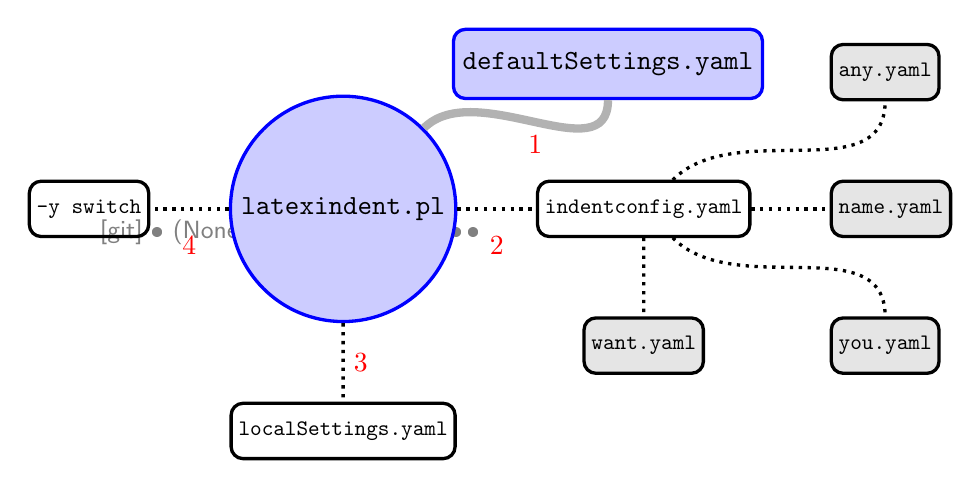
\begin{tikzpicture}[
		needed/.style={very thick, draw=blue,fill=blue!20, text centered, minimum height=2.5em,rounded corners=1ex},
		optional/.style={draw=black, very thick,scale=0.8, text centered, minimum height=2.5em,rounded corners=1ex},
		optionalfill/.style={fill=black!10},
		connections/.style={draw=black!30,dotted,line width=3pt,text=red},
	]
	% Draw diagram elements
	\node (latexindent) [needed,circle] {\texttt{latexindent.pl}};
	\node (default) [needed,above right=.5cm of latexindent] {\texttt{defaultSettings.yaml}};
	\node (indentconfig) [optional,right=of latexindent] {\texttt{indentconfig.yaml}};
	\node (any) [optional,optionalfill,above right=of indentconfig] {\texttt{any.yaml}};
	\node (name) [optional,optionalfill,right=of indentconfig] {\texttt{name.yaml}};
	\node (you) [optional,optionalfill,below right=of indentconfig] {\texttt{you.yaml}};
	\node (want) [optional,optionalfill,below=of indentconfig] {\texttt{want.yaml}};
	\node (local) [optional,below=of latexindent] {\texttt{localSettings.yaml}};
	\node (yamlswitch) [optional,left=of latexindent] {\texttt{-y switch}};
	% Draw arrows between elements
	\draw[connections,solid] (latexindent) to[in=-90]node[pos=0.5,anchor=north]{1} (default.south) ;
	\draw[connections,optional] (latexindent) -- node[pos=0.5,anchor=north]{2} (indentconfig) ;
	\draw[connections,optional] (indentconfig) to[in=-90] (any.south) ;
	\draw[connections,optional] (indentconfig) -- (name) ;
	\draw[connections,optional] (indentconfig) to[out=-45,in=90] (you) ;
	\draw[connections,optional] (indentconfig) -- (want) ;
	\draw[connections,optional] (latexindent) -- node[pos=0.5,anchor=west]{3} (local) ;
	\draw[connections,optional] (latexindent) -- node[pos=0.5,anchor=north]{4} (yamlswitch) ;
\end{tikzpicture}
\end{document}

		\caption{Schematic of the load order described in \cref{sec:loadorder}; solid lines represent
			mandatory files, dotted lines represent optional files. \texttt{indentconfig.yaml} can
			contain as many files as you like. The files will be loaded in order; if you specify
			settings for the same field in more than one file, the most recent takes priority. }
		\label{fig:loadorder}
	\end{figure}

 % arara: pdflatex: {shell: yes, files: [latexindent]}
\section{defaultSettings.yaml}\label{sec:defuseloc}
 \texttt{latexindent.pl} loads its settings from \texttt{defaultSettings.yaml}. The idea is to
 separate the behaviour of the script from the internal working -- this is very similar to
 the way that we separate content from form when writing our documents in \LaTeX.

 If you look in \texttt{defaultSettings.yaml} you'll find the switches that govern the behaviour
 of \texttt{latexindent.pl}. If you're not sure where \texttt{defaultSettings.yaml} resides on
 your computer, don't worry as \texttt{indent.log} will tell you where to find it.
 \texttt{defaultSettings.yaml} is commented, but here is a description of what each switch is
 designed to do. The default value is given in each case; whenever you see
 \emph{integer} in \emph{this} section, assume that it must be
 greater than or equal to \texttt{0} unless otherwise stated.

\yamltitle{fileExtensionPreference}*{fields}
	\texttt{latexindent.pl} can be called to
	act on a file without specifying the file extension.  For example we can call
	\begin{commandshell}
latexindent.pl myfile
\end{commandshell}
	\begin{wrapfigure}[8]{r}[0pt]{6cm}
		\cmhlistingsfromfile[style=fileExtensionPreference]*{../defaultSettings.yaml}[width=.8\linewidth,before=\centering,yaml-TCB]{\texttt{fileExtensionPreference}}{lst:fileExtensionPreference}
	\end{wrapfigure}

	in which case the script will look for \texttt{myfile} with the extensions
	specified in \texttt{fileExtensionPreference} in their numeric order. If no match is found, the
	script will exit. As with all of the fields, you should change and/or add to this as
	necessary.

	Calling \texttt{latexindent.pl myfile} with the (default) settings specified in
	\cref{lst:fileExtensionPreference} means that the script will first look for
	\texttt{myfile.tex}, then \texttt{myfile.sty}, \texttt{myfile.cls}, and
	finally \texttt{myfile.bib} in order\footnote{Throughout this manual, listings shown with line numbers represent code
		taken directly from \texttt{defaultSettings.yaml}.}.

\yamltitle{backupExtension}*{extension name}

	If you call \texttt{latexindent.pl} with the \texttt{-w} switch (to overwrite
	\texttt{myfile.tex}) then it will create a backup file before doing any indentation;
	the default extension is \texttt{.bak}, so, for example,
	\texttt{myfile.bak0} would be created when calling \texttt{latexindent.pl myfile.tex} for the
	first time.

	By default, every time you subsequently call \texttt{latexindent.pl} with the
	\texttt{-w} to act upon \texttt{myfile.tex}, it will create successive
	back up files: \texttt{myfile.bak1}, \texttt{myfile.bak2}, etc.

\yamltitle{onlyOneBackUp}*{integer}
	\label{page:onlyonebackup}
	If you don't want a backup for every time that you call \texttt{latexindent.pl} (so
	you don't want \texttt{myfile.bak1}, \texttt{myfile.bak2}, etc) and you
	simply want \texttt{myfile.bak} (or whatever you chose \texttt{backupExtension} to be) then change \texttt{onlyOneBackUp} to
	\texttt{1}; the default value of \texttt{onlyOneBackUp} is
	\texttt{0}.

\yamltitle{maxNumberOfBackUps}*{integer}
	Some users may only want a finite number of backup files, say at most
	$3$, in which case, they can change this switch. The smallest value of
	\texttt{maxNumberOfBackUps} is $0$ which will \emph{not}
	prevent backup files being made; in this case, the behaviour will be dictated entirely by
	\texttt{onlyOneBackUp}. The default value of \texttt{maxNumberOfBackUps} is
	\texttt{0}.

\yamltitle{cycleThroughBackUps}*{integer}
	Some users may wish to cycle through backup files, by deleting the oldest backup file and
	keeping only the most recent; for example, with \texttt{maxNumberOfBackUps: 4}, and
	\texttt{cycleThroughBackUps} set to \texttt{1} then the \texttt{copy}
	procedure given below would be obeyed.

	\begin{commandshell}
copy myfile.bak1 to myfile.bak0
copy myfile.bak2 to myfile.bak1
copy myfile.bak3 to myfile.bak2
copy myfile.bak4 to myfile.bak3
\end{commandshell}
	The default value of \texttt{cycleThroughBackUps} is \texttt{0}.

\yamltitle{logFilePreferences}*{fields}
	\texttt{latexindent.pl} writes information to \texttt{indent.log}, some
	of which can be customized by changing \texttt{logFilePreferences}; see
	\cref{lst:logFilePreferences}. If you load your own user settings (see \vref{sec:indentconfig})
	then \texttt{latexindent.pl} will detail them in \texttt{indent.log}; you can choose
	not to have the details logged by switching \texttt{showEveryYamlRead} to
	\texttt{0}. Once all of your settings have been loaded, you can see the
	amalgamated settings in the log file by switching \texttt{showAmalgamatedSettings} to
	\texttt{1}, if you wish.

	\cmhlistingsfromfile[style=logFilePreferences,]*{../defaultSettings.yaml}[width=.9\linewidth,before=\centering,yaml-TCB]{\texttt{logFilePreferences}}{lst:logFilePreferences}

	When%
	\announce{2018-01-13}{showDecorationStartCodeBlockTrace feature for log file} either of the
	\texttt{trace} modes (see \cpageref{page:traceswitch}) are active, you will receive
	detailed information in \texttt{indent.log}. You can specify character strings to
	appear before and after the notification of a found code block using, respectively,
	\texttt{showDecorationStartCodeBlockTrace} and \texttt{showDecorationFinishCodeBlockTrace}. A demonstration is given in
	\vref{app:logfile-demo}.

	The log file will end with the characters given in \texttt{endLogFileWith}, and will
	report the \texttt{GitHub} address of \texttt{latexindent.pl} to the log file if
	\texttt{showGitHubInfoFooter} is set to \texttt{1}.

	\texttt{latexindent.pl}%
	\announce{2018-01-13}{log file pattern layout for log file} uses the \texttt{log4perl} module \cite{log4perl}
	to handle the creation of the logfile. You can specify the layout of the information
	given in the logfile using any of the \texttt{Log Layouts} detailed at
	\cite{log4perl}.

\yamltitle{verbatimEnvironments}*{fields}

	A field that contains a list of environments that you would like left completely alone --
	no indentation will be performed on environments that you have specified in this field,
	see \cref{lst:verbatimEnvironments}.

	\begin{cmhtcbraster}[raster column skip=.1\linewidth]
		\cmhlistingsfromfile[style=verbatimEnvironments]*{../defaultSettings.yaml}[width=.8\linewidth,before=\centering,yaml-TCB]{\texttt{verbatimEnvironments}}{lst:verbatimEnvironments}
		\cmhlistingsfromfile[style=verbatimCommands]*{../defaultSettings.yaml}[width=.8\linewidth,before=\centering,yaml-TCB]{\texttt{verbatimCommands}}{lst:verbatimCommands}
	\end{cmhtcbraster}

	Note that if you put an environment in	\texttt{verbatimEnvironments} and in other fields such
	as \texttt{lookForAlignDelims} or \texttt{noAdditionalIndent} then \texttt{latexindent.pl} will
	\emph{always} prioritize  \texttt{verbatimEnvironments}.

\yamltitle{verbatimCommands}*{fields}
	A field that contains a list of commands that are verbatim commands, for example
	\lstinline|\lstinline|; any commands populated in this field are protected from line
	breaking routines (only relevant if the \texttt{-m} is active, see
	\vref{sec:modifylinebreaks}).

\yamltitle{noIndentBlock}*{fields}

	\begin{wrapfigure}[8]{r}[0pt]{6cm}
		\cmhlistingsfromfile[style=noIndentBlock]*{../defaultSettings.yaml}[width=.8\linewidth,before=\centering,yaml-TCB]{\texttt{noIndentBlock}}{lst:noIndentBlock}
	\end{wrapfigure}
	If you have a block of code that you don't want \texttt{latexindent.pl} to touch (even if
	it is \emph{not} a verbatim-like environment) then you can wrap it in an
	environment from \texttt{noIndentBlock}; you can use any name you like for this,
	provided you populate it as demonstrate in \cref{lst:noIndentBlock}.

	Of course, you don't want to have to specify these as null environments in your code, so
	you use them with a comment symbol, \lstinline!%!, followed by as many spaces
	(possibly none) as you like; see \cref{lst:noIndentBlockdemo} for example.

	\begin{cmhlistings}[style=demo,escapeinside={(*@}{@*)}]{\texttt{noIndentBlock} demonstration}{lst:noIndentBlockdemo}
%(*@@*) \begin{noindent}
        this code
                won't
     be touched
                    by
             latexindent.pl!
%(*@@*)\end{noindent}
	\end{cmhlistings}

\yamltitle{removeTrailingWhitespace}*{fields}\label{yaml:removeTrailingWhitespace}

	\begin{wrapfigure}[10]{r}[0pt]{7cm}
		\cmhlistingsfromfile[style=removeTrailingWhitespace]*{../defaultSettings.yaml}[width=.8\linewidth,before=\centering,yaml-TCB]{removeTrailingWhitespace}{lst:removeTrailingWhitespace}

		\vspace{.1cm}
		\begin{yaml}[numbers=none]{removeTrailingWhitespace (alt)}[width=.8\linewidth,before=\centering]{lst:removeTrailingWhitespace-alt}
removeTrailingWhitespace: 1
\end{yaml}
	\end{wrapfigure}
	Trailing white space can be removed both \emph{before} and
	\emph{after} processing the document, as detailed in \cref{lst:removeTrailingWhitespace};
	each of the fields can take the values \texttt{0} or
	\texttt{1}. See \vref{lst:removeTWS-before,lst:env-mlb5-modAll,lst:env-mlb5-modAll-remove-WS} for before and after results. Thanks
	to \cite{vosskuhle} for providing this feature.

	You can specify \texttt{removeTrailingWhitespace} simply as \texttt{0} or
	\texttt{1}, if you wish; in this case,%
	\announce{2017-06-28}{removeTrailingWhitespace} \texttt{latexindent.pl} will set both \texttt{beforeProcessing} and
	\texttt{afterProcessing} to the value you specify; see \cref{lst:removeTrailingWhitespace-alt}.
\yamltitle{fileContentsEnvironments}*{field}

	\begin{wrapfigure}[6]{r}[0pt]{6cm}
		\cmhlistingsfromfile[style=fileContentsEnvironments]*{../defaultSettings.yaml}[width=.8\linewidth,before=\centering,yaml-TCB]{\texttt{fileContentsEnvironments}}{lst:fileContentsEnvironments}
	\end{wrapfigure}
	Before \texttt{latexindent.pl} determines the difference between preamble (if any) and
	the main document, it first searches for any of the environments specified in
	\texttt{fileContentsEnvironments}, see \cref{lst:fileContentsEnvironments}. The behaviour of
	\texttt{latexindent.pl} on these environments is determined by their location (preamble
	or not), and the value \texttt{indentPreamble}, discussed next.

\yamltitle{indentPreamble}{0|1}

	The preamble of a document can sometimes contain some trickier code for
	\texttt{latexindent.pl} to operate upon. By default, \texttt{latexindent.pl} won't try to
	operate on the preamble (as \texttt{indentPreamble} is set to \texttt{0}, by
	default), but if you'd like \texttt{latexindent.pl} to try then change
	\texttt{indentPreamble} to \texttt{1}.

\yamltitle{lookForPreamble}*{fields}

	\begin{wrapfigure}[8]{r}[0pt]{5cm}
		\cmhlistingsfromfile[style=lookForPreamble]*{../defaultSettings.yaml}[width=.8\linewidth,before=\centering,yaml-TCB]{lookForPreamble}{lst:lookForPreamble}
	\end{wrapfigure}
	Not all files contain preamble; for example, \texttt{sty},
	\texttt{cls} and \texttt{bib} files typically do
	\emph{not}. Referencing \cref{lst:lookForPreamble}, if you set, for example,
	\texttt{.tex} to \texttt{0}, then regardless of the setting of the
	value of \texttt{indentPreamble}, preamble will not be assumed when operating upon
	\texttt{.tex} files.
\yamltitle{preambleCommandsBeforeEnvironments}{0|1}
	Assuming that \texttt{latexindent.pl} is asked to operate upon the preamble of a
	document, when this switch is set to \texttt{0} then environment code blocks
	will be sought first, and then command code blocks. When this switch is set to
	\texttt{1}, commands will be sought first. The example that first motivated
	this switch contained the code given in \cref{lst:motivatepreambleCommandsBeforeEnvironments}.

	\begin{cmhlistings}{Motivating \texttt{preambleCommandsBeforeEnvironments}}{lst:motivatepreambleCommandsBeforeEnvironments}
...
preheadhook={\begin{mdframed}[style=myframedstyle]},
postfoothook=\end{mdframed},
...
\end{cmhlistings}

\yamltitle{defaultIndent}*{horizontal space}
	This is the default indentation (\lstinline!\t! means a tab, and is the default
	value) used in the absence of other details for the command or environment we are working
	with; see \texttt{indentRules} in \vref{sec:noadd-indent-rules} for more details.

	If you're interested in experimenting with \texttt{latexindent.pl} then you can
	\emph{remove} all indentation by setting \texttt{defaultIndent: ""}.

\yamltitle{lookForAlignDelims}*{fields}\label{yaml:lookforaligndelims}
	\begin{wrapfigure}[12]{r}[0pt]{5cm}
		\begin{yaml}[numbers=none]{\texttt{lookForAlignDelims} (basic)}[width=.8\linewidth,before=\centering]{lst:aligndelims:basic}
lookForAlignDelims:
   tabular: 1
   tabularx: 1
   longtable: 1
   array: 1
   matrix: 1
   ...
	\end{yaml}
	\end{wrapfigure}
	This contains a list of environments and/or commands that are operated upon in a special
	way by \texttt{latexindent.pl} (see \cref{lst:aligndelims:basic}). In fact, the fields in \texttt{lookForAlignDelims} can
	actually take two different forms: the \emph{basic} version is shown in
	\cref{lst:aligndelims:basic} and the \emph{advanced} version in
	\cref{lst:aligndelims:advanced}; we will discuss each in turn.

	The environments specified in this field will be operated on in a special way by
	\texttt{latexindent.pl}. In particular, it will try and align each column by its
	alignment tabs. It does have some limitations (discussed further in
	\cref{sec:knownlimitations}), but in many cases it will produce results such as those in
	\cref{lst:tabularbefore:basic,lst:tabularafter:basic}.

	If you find that \texttt{latexindent.pl} does not perform satisfactorily on such
	environments then you can set the relevant key to \texttt{0}, for example
	\texttt{tabular: 0}; alternatively, if you just want to ignore
	\emph{specific} instances of the environment, you could wrap them in something
	from \texttt{noIndentBlock} (see \vref{lst:noIndentBlock}).

	\begin{cmhtcbraster}
		\cmhlistingsfromfile{demonstrations/tabular1.tex}{\texttt{tabular1.tex}}{lst:tabularbefore:basic}
		\cmhlistingsfromfile{demonstrations/tabular1-default.tex}{\texttt{tabular1.tex} default output}{lst:tabularafter:basic}
	\end{cmhtcbraster}

	If, for example, you wish to remove the alignment of the \lstinline!\\! within a
	delimiter-aligned block, then the advanced form of \texttt{lookForAlignDelims} shown in
	\cref{lst:aligndelims:advanced} is for you.

	\cmhlistingsfromfile[style=yaml-LST]*{demonstrations/tabular.yaml}[yaml-TCB]{\texttt{tabular.yaml}}{lst:aligndelims:advanced}

	Note that you can use a mixture of the basic and advanced form: in
	\cref{lst:aligndelims:advanced} \texttt{tabular} and \texttt{tabularx} are advanced
	and \texttt{longtable} is basic. When using the advanced form, each field should
	receive at least 1 sub-field, and \emph{can}
	(but does not have to) receive any of the following
	fields:
	\begin{itemize}
		\item \texttt{delims}: binary switch (0 or 1) equivalent to simply specifying, for
		      example, \texttt{tabular: 1} in the basic version shown in \cref{lst:aligndelims:basic}. If
		      \texttt{delims} is set to \texttt{0} then the align at ampersand
		      routine will not be called for this code block (default: 1);
		\item \texttt{alignDoubleBackSlash}: binary switch (0 or 1) to determine if \lstinline!\\!
		      should be aligned (default: 1);
		\item \texttt{spacesBeforeDoubleBackSlash}: optionally,%
		      \announce{2018-01-13}*{update to spacesBeforeDoubleBackSlash in ampersand alignment} specifies the number (integer $\geq$ 0) of spaces
		      to be inserted before \lstinline!\\! (default: 1). \footnote{Previously this only activated if \texttt{alignDoubleBackSlash} was set to \texttt{0}.}
		\item \announce{2017-06-19}{multiColumnGrouping} \texttt{multiColumnGrouping}: binary switch (0 or 1) that details if
		      \texttt{latexindent.pl} should group columns
		      above and below a \lstinline!\multicolumn! command (default: 0);
		\item \announce{2017-06-19}{alignRowsWithoutMaxDelims} \texttt{alignRowsWithoutMaxDelims}: binary switch (0 or 1) that details if
		      rows that do not contain the maximum number of delimeters should be formatted so as to
		      have the ampersands aligned (default: 1);
		\item \announce{2018-01-13}{spacesBeforeAmpersand in ampersand alignment}\texttt{spacesBeforeAmpersand}: optionally specifies the number (integer
		      $\geq$ 0) of
		      spaces to be placed \emph{before} ampersands (default: 1);
		\item \announce{2018-01-13}{spacesAfterAmpersand in ampersand alignment}\texttt{spacesAfterAmpersand}: optionally specifies the number (integer
		      $\geq$ 0) of
		      spaces to be placed \emph{After} ampersands (default: 1);
		\item \announce{2018-01-13}{justification of cells in ampersand alignment}\texttt{justification}: optionally specifies the justification of
		      each cell as either \emph{left} or \emph{right} (default: left).
	\end{itemize}

	We will explore each of these features using the file \texttt{tabular2.tex} in
	\cref{lst:tabular2} (which contains a \lstinline!\multicolumn! command), and the YAML files in \crefrange{lst:tabular2YAML}{lst:tabular8YAML}.

	\cmhlistingsfromfile{demonstrations/tabular2.tex}{\texttt{tabular2.tex}}{lst:tabular2}
	\begin{minipage}{.45\textwidth}
		\cmhlistingsfromfile[style=yaml-LST]*{demonstrations/tabular2.yaml}[yaml-TCB]{\texttt{tabular2.yaml}}{lst:tabular2YAML}
	\end{minipage}%
	\hfill
	\begin{minipage}{.48\textwidth}
		\cmhlistingsfromfile[style=yaml-LST]*{demonstrations/tabular3.yaml}[yaml-TCB]{\texttt{tabular3.yaml}}{lst:tabular3YAML}
	\end{minipage}%

	\begin{minipage}{.45\textwidth}
		\cmhlistingsfromfile[style=yaml-LST]*{demonstrations/tabular4.yaml}[yaml-TCB]{\texttt{tabular4.yaml}}{lst:tabular4YAML}
	\end{minipage}%
	\hfill
	\begin{minipage}{.48\textwidth}
		\cmhlistingsfromfile[style=yaml-LST]*{demonstrations/tabular5.yaml}[yaml-TCB]{\texttt{tabular5.yaml}}{lst:tabular5YAML}
	\end{minipage}%

	\begin{minipage}{.45\textwidth}
		\cmhlistingsfromfile[style=yaml-LST]*{demonstrations/tabular6.yaml}[yaml-TCB]{\texttt{tabular6.yaml}}{lst:tabular6YAML}
	\end{minipage}%
	\hfill
	\begin{minipage}{.48\textwidth}
		\cmhlistingsfromfile[style=yaml-LST]*{demonstrations/tabular7.yaml}[yaml-TCB]{\texttt{tabular7.yaml}}{lst:tabular7YAML}
	\end{minipage}%

	\begin{minipage}{.48\textwidth}
		\cmhlistingsfromfile[style=yaml-LST]*{demonstrations/tabular8.yaml}[yaml-TCB]{\texttt{tabular8.yaml}}{lst:tabular8YAML}
	\end{minipage}%

	On running the commands
	\begin{commandshell}
latexindent.pl tabular2.tex 
latexindent.pl tabular2.tex -l tabular2.yaml
latexindent.pl tabular2.tex -l tabular3.yaml
latexindent.pl tabular2.tex -l tabular2.yaml,tabular4.yaml
latexindent.pl tabular2.tex -l tabular2.yaml,tabular5.yaml
latexindent.pl tabular2.tex -l tabular2.yaml,tabular6.yaml
latexindent.pl tabular2.tex -l tabular2.yaml,tabular7.yaml
latexindent.pl tabular2.tex -l tabular2.yaml,tabular8.yaml
\end{commandshell}
	we obtain the respective outputs given in \crefrange{lst:tabular2-default}{lst:tabular2-mod8}.

	\begin{widepage}
		\cmhlistingsfromfile{demonstrations/tabular2-default.tex}{\texttt{tabular2.tex} default output}{lst:tabular2-default}
		\cmhlistingsfromfile{demonstrations/tabular2-mod2.tex}{\texttt{tabular2.tex} using \cref{lst:tabular2YAML}}{lst:tabular2-mod2}
		\cmhlistingsfromfile{demonstrations/tabular2-mod3.tex}{\texttt{tabular2.tex} using \cref{lst:tabular3YAML}}{lst:tabular2-mod3}
		\cmhlistingsfromfile{demonstrations/tabular2-mod4.tex}{\texttt{tabular2.tex} using \cref{lst:tabular2YAML,lst:tabular4YAML}}{lst:tabular2-mod4}
		\cmhlistingsfromfile{demonstrations/tabular2-mod5.tex}{\texttt{tabular2.tex} using \cref{lst:tabular2YAML,lst:tabular5YAML}}{lst:tabular2-mod5}
		\cmhlistingsfromfile{demonstrations/tabular2-mod6.tex}{\texttt{tabular2.tex} using \cref{lst:tabular2YAML,lst:tabular6YAML}}{lst:tabular2-mod6}
		\cmhlistingsfromfile{demonstrations/tabular2-mod7.tex}{\texttt{tabular2.tex} using \cref{lst:tabular2YAML,lst:tabular7YAML}}{lst:tabular2-mod7}
		\cmhlistingsfromfile{demonstrations/tabular2-mod8.tex}{\texttt{tabular2.tex} using \cref{lst:tabular2YAML,lst:tabular8YAML}}{lst:tabular2-mod8}
	\end{widepage}

	Notice in particular:
	\begin{itemize}
		\item in both \cref{lst:tabular2-default,lst:tabular2-mod2} all rows have been aligned at the ampersand, even those
		      that do not contain the maximum number of ampersands (3 ampersands, in this case);
		\item in \cref{lst:tabular2-default} the columns have been aligned at the ampersand;
		\item in \cref{lst:tabular2-mod2} the \lstinline!\multicolumn! command has grouped the
		      $2$ columns beneath \emph{and} above it, because
		      \texttt{multiColumnGrouping} is set to $1$ in \cref{lst:tabular2YAML};
		\item in \cref{lst:tabular2-mod3} rows~3 and~6 have \emph{not} been aligned at the
		      ampersand, because \texttt{alignRowsWithoutMaxDelims} has been to set to $0$ in
		      \cref{lst:tabular3YAML}; however, the \lstinline!\\! \emph{have} still
		      been aligned;
		\item in \cref{lst:tabular2-mod4} the columns beneath and above the \lstinline!\multicolumn!
		      commands have been grouped (because \texttt{multiColumnGrouping} is set to
		      $1$), and there are at least $4$ spaces
		      \emph{before} each aligned ampersand because \texttt{spacesBeforeAmpersand} is set to
		      $4$;
		\item in \cref{lst:tabular2-mod5} the columns beneath and above the \lstinline!\multicolumn!
		      commands have been grouped (because \texttt{multiColumnGrouping} is set to
		      $1$), and there are at least $4$ spaces
		      \emph{after} each aligned ampersand because \texttt{spacesAfterAmpersand} is set to
		      $4$;
		\item in \cref{lst:tabular2-mod6} the \lstinline!\\! have \emph{not} been
		      aligned, because \texttt{alignDoubleBackSlash} is set to \texttt{0}, otherwise the
		      output is the same as \cref{lst:tabular2-mod2};
		\item in \cref{lst:tabular2-mod7} the \lstinline!\\! \emph{have} been
		      aligned, and because \texttt{spacesBeforeDoubleBackSlash} is set to \texttt{0}, there are
		      no spaces ahead of them; the output is otherwise the same as \cref{lst:tabular2-mod2}.
		\item in \cref{lst:tabular2-mod8} the cells have been \emph{right}-justified; note
		      that cells above and below the \lstinline!\multicol! statements have still been group
		      correctly, because of the settings in \cref{lst:tabular2YAML}.
	\end{itemize}

	As of Version 3.0, the alignment routine works on mandatory and optional arguments within
	commands, and also within `special' code blocks (see \texttt{specialBeginEnd} on
	\cpageref{yaml:specialBeginEnd}); for example, assuming that you have a command called
	\lstinline!\matrix! and that it is populated within \texttt{lookForAlignDelims} (which it is, by default), and that
	you run the command
	\begin{commandshell}
latexindent.pl matrix1.tex 
\end{commandshell}
	then the before-and-after results shown in \cref{lst:matrixbefore,lst:matrixafter} are achievable by
	default.

	\begin{cmhtcbraster}
		\cmhlistingsfromfile{demonstrations/matrix1.tex}{\texttt{matrix1.tex}}{lst:matrixbefore}
		\cmhlistingsfromfile{demonstrations/matrix1-default.tex}{\texttt{matrix1.tex} default output}{lst:matrixafter}
	\end{cmhtcbraster}

	If you have blocks of code that you wish to align at the \&  character that are
	\emph{not} wrapped in, for example, \lstinline!\begin{tabular}! \ldots
	\lstinline!\end{tabular}!, then you can use the mark up illustrated in
	\cref{lst:alignmentmarkup}; the default output is shown in \cref{lst:alignmentmarkup-default}. Note
	that the \lstinline!%*! must be next to each other, but that there can be any
	number of spaces (possibly none) between the
	\lstinline!*! and \lstinline!\begin{tabular}!; note also that you may use any
	environment name that you have specified in \texttt{lookForAlignDelims}.

	\begin{cmhtcbraster}
		\cmhlistingsfromfile{demonstrations/align-block.tex}{\texttt{align-block.tex}}{lst:alignmentmarkup}
		\cmhlistingsfromfile{demonstrations/align-block-default.tex}{\texttt{align-block.tex} default output}{lst:alignmentmarkup-default}
	\end{cmhtcbraster}

	With reference to \vref{tab:code-blocks} and the, yet undiscussed, fields of
	\texttt{noAdditionalIndent} and \texttt{indentRules}
	(see \vref{sec:noadd-indent-rules}), these comment-marked blocks are
	considered \texttt{environments}.

\yamltitle{indentAfterItems}*{fields}
	The environment names specified in \texttt{indentAfterItems} tell \texttt{latexindent.pl}
	to look for \lstinline!\item! commands; if these switches are set to
	\texttt{1} then indentation will be performed so as indent the code after
	each \texttt{item}. A demonstration is given in \cref{lst:itemsbefore,lst:itemsafter}

	\begin{cmhtcbraster}[raster columns=3,
			raster left skip=-3.5cm,
			raster right skip=-2cm,
			raster column skip=.03\linewidth]
		\cmhlistingsfromfile[style=indentAfterItems]*{../defaultSettings.yaml}[width=.8\linewidth,before=\centering,yaml-TCB]{\texttt{indentAfterItems}}{lst:indentafteritems}
		\cmhlistingsfromfile{demonstrations/items1.tex}{\texttt{items1.tex}}{lst:itemsbefore}
		\cmhlistingsfromfile{demonstrations/items1-default.tex}{\texttt{items1.tex} default output}{lst:itemsafter}
	\end{cmhtcbraster}

\yamltitle{itemNames}*{fields}
	\begin{wrapfigure}[5]{r}[0pt]{5cm}
		\cmhlistingsfromfile[style=itemNames]*{../defaultSettings.yaml}[width=.8\linewidth,before=\centering,yaml-TCB]{\texttt{itemNames}}{lst:itemNames}
	\end{wrapfigure}
	If you have your own \texttt{item} commands (perhaps you prefer to use
	\texttt{myitem}, for example) then you can put populate them in
	\texttt{itemNames}. For example, users of the \texttt{exam} document class
	might like to add \texttt{parts} to \texttt{indentAfterItems} and
	\texttt{part} to \texttt{itemNames} to their user settings (see
	\vref{sec:indentconfig} for details of how to configure user settings, and
	\vref{lst:mysettings} \\ in particular \label{page:examsettings}.)

\yamltitle{specialBeginEnd}*{fields}\label{yaml:specialBeginEnd}
	The fields specified%
	\announce{2017-08-21}*{specialBeginEnd} in
	\texttt{specialBeginEnd} are, in their default state, focused on math mode begin and end
	statements, but there is no requirement for this to be the case; \cref{lst:specialBeginEnd}
	shows the default settings of \texttt{specialBeginEnd}.

	\cmhlistingsfromfile[style=specialBeginEnd]*{../defaultSettings.yaml}[width=.8\linewidth,before=\centering,yaml-TCB]{\texttt{specialBeginEnd}}{lst:specialBeginEnd}

	The field \texttt{displayMath} represents \lstinline!\[...\]!,
	\texttt{inlineMath} represents
	\lstinline!$...$! and \texttt{displayMathTex} represents \lstinline!$$...$$!.
	You can, of course, rename these in your own YAML files (see \vref{sec:localsettings});
	indeed, you might like to set up your own special begin and end statements.

	A demonstration of the before-and-after results are shown in \cref{lst:specialbefore,lst:specialafter}.

	\begin{cmhtcbraster}
		\cmhlistingsfromfile{demonstrations/special1.tex}{\texttt{special1.tex} before}{lst:specialbefore}
		\cmhlistingsfromfile{demonstrations/special1-default.tex}{\texttt{special1.tex} default output}{lst:specialafter}
	\end{cmhtcbraster}

	For each field, \texttt{lookForThis} is set to \texttt{1} by default,
	which means that \texttt{latexindent.pl} will look for this pattern; you can tell
	\texttt{latexindent.pl} not to look for the pattern, by setting \texttt{lookForThis}
	to \texttt{0}.

	There are%
	\announce{2017-08-21}{specialBeforeCommand} examples in which it
	is advantageous to search for \texttt{specialBeginEnd} fields \emph{before}
	searching for commands, and the \texttt{specialBeforeCommand} switch controls this behaviour.
	For example, consider the file shown in \cref{lst:specialLRbefore}.

	\cmhlistingsfromfile{demonstrations/specialLR.tex}{\texttt{specialLR.tex}}{lst:specialLRbefore}

	Now consider the YAML files shown in \cref{lst:specialsLeftRight-yaml,lst:specialBeforeCommand-yaml}

	\begin{cmhtcbraster}
		\cmhlistingsfromfile[]*{demonstrations/specialsLeftRight.yaml}[width=.8\linewidth,before=\centering,yaml-TCB]{\texttt{specialsLeftRight.yaml}}{lst:specialsLeftRight-yaml}
		\cmhlistingsfromfile[]*{demonstrations/specialBeforeCommand.yaml}[width=.8\linewidth,before=\centering,yaml-TCB]{\texttt{specialBeforeCommand.yaml}}{lst:specialBeforeCommand-yaml}
	\end{cmhtcbraster}

	Upon running the following commands
	\begin{widepage}
		\begin{commandshell}
latexindent.pl specialLR.tex -l=specialsLeftRight.yaml      
latexindent.pl specialLR.tex -l=specialsLeftRight.yaml,specialBeforeCommand.yaml      
\end{commandshell}
	\end{widepage}
	we receive the respective outputs in \cref{lst:specialLR-comm-first-tex,lst:specialLR-special-first-tex}.

	\begin{minipage}{.49\linewidth}
		\cmhlistingsfromfile{demonstrations/specialLR-comm-first.tex}{\texttt{specialLR.tex} using \cref{lst:specialsLeftRight-yaml}}{lst:specialLR-comm-first-tex}
	\end{minipage}
	\hfill
	\begin{minipage}{.49\linewidth}
		\cmhlistingsfromfile{demonstrations/specialLR-special-first.tex}{\texttt{specialLR.tex} using \cref{lst:specialsLeftRight-yaml,lst:specialBeforeCommand-yaml}}{lst:specialLR-special-first-tex}
	\end{minipage}

	Notice that in:
	\begin{itemize}
		\item \cref{lst:specialLR-comm-first-tex} the \lstinline!\left! has been treated as a
		      \emph{command}, with one optional argument;
		\item \cref{lst:specialLR-special-first-tex} the \texttt{specialBeginEnd} pattern in \cref{lst:specialsLeftRight-yaml}
		      has been obeyed because \cref{lst:specialBeforeCommand-yaml} specifies that the
		      \texttt{specialBeginEnd} should be sought \emph{before} commands.
	\end{itemize}

	You can,optionally, specify%
	\announce{2018-04-27}{update to specialBeginEnd} the
	\texttt{middle} field for anything that you specify in \texttt{specialBeginEnd}.
	For example, let's consider the \texttt{.tex} file in \cref{lst:special2}.

	\cmhlistingsfromfile{demonstrations/special2.tex}{\texttt{special2.tex}}{lst:special2}

	Upon saving the YAML settings in \cref{lst:middle-yaml,lst:middle1-yaml} and running the commands
	\begin{commandshell}
latexindent.pl special2.tex -l=middle
latexindent.pl special2.tex -l=middle1
\end{commandshell}
	then we obtain the output given in \cref{lst:special2-mod1,lst:special2-mod2}.

	\begin{cmhtcbraster}
		\cmhlistingsfromfile{demonstrations/middle.yaml}[yaml-TCB]{\texttt{middle.yaml}}{lst:middle-yaml}
		\cmhlistingsfromfile{demonstrations/special2-mod1.tex}{\texttt{special2.tex} using \cref{lst:middle-yaml}}{lst:special2-mod1}
	\end{cmhtcbraster}

	\begin{cmhtcbraster}
		\cmhlistingsfromfile{demonstrations/middle1.yaml}[yaml-TCB]{\texttt{middle1.yaml}}{lst:middle1-yaml}
		\cmhlistingsfromfile{demonstrations/special2-mod2.tex}{\texttt{special2.tex} using \cref{lst:middle1-yaml}}{lst:special2-mod2}
	\end{cmhtcbraster}

	We note that:
	\begin{itemize}
		\item in \cref{lst:special2-mod1} the bodies of each of the \texttt{Elsif} statements
		      have been indented appropriately;
		\item the \texttt{Else} statement has \emph{not} been indented
		      appropriately in \cref{lst:special2-mod1} -- read on!
		\item we have specified multiple settings for the \texttt{middle} field using the
		      syntax demonstrated in \cref{lst:middle1-yaml} so that the body of the
		      \texttt{Else} statement has been indented appropriately in
		      \cref{lst:special2-mod2}.
	\end{itemize}

	You may%
	\announce{2018-08-13}{specialBeginEnd verbatim} specify fields in
	\texttt{specialBeginEnd} to be treated as verbatim code blocks by changing
	\texttt{lookForThis} to be \texttt{verbatim}.

	For example, beginning with the code in \cref{lst:special3-mod1} and the YAML in
	\cref{lst:special-verb1-yaml}, and running
	\begin{commandshell}
latexindent.pl special3.tex -l=special-verb1
\end{commandshell}
	then the output in \cref{lst:special3-mod1} is unchanged.

	\begin{cmhtcbraster}
		\cmhlistingsfromfile{demonstrations/special-verb1.yaml}[yaml-TCB]{\texttt{special-verb1.yaml}}{lst:special-verb1-yaml}
		\cmhlistingsfromfile{demonstrations/special3-mod1.tex}{\texttt{special3.tex} and output using \cref{lst:special-verb1-yaml}}{lst:special3-mod1}
	\end{cmhtcbraster}

\yamltitle{indentAfterHeadings}*{fields}
	\begin{wrapfigure}[17]{r}[0pt]{8cm}
		\cmhlistingsfromfile[style=indentAfterHeadings]*{../defaultSettings.yaml}[width=.8\linewidth,before=\centering,yaml-TCB]{\texttt{indentAfterHeadings}}{lst:indentAfterHeadings}
	\end{wrapfigure}
	This field enables the user to specify indentation rules that take effect after heading
	commands such as \lstinline!\part!, \lstinline!\chapter!,
	\lstinline!\section!, \lstinline!\subsection*!, or indeed any user-specified command
	written in this field.\footnote{There is a slight
		difference in interface for this field when comparing Version 2.2 to Version 3.0; see \vref{app:differences} for details.}

	The default settings do \emph{not} place indentation after a heading, but
	you can easily switch them on by changing \\ \texttt{indentAfterThisHeading: 0} to \\
	\texttt{indentAfterThisHeading: 1}. The \texttt{level} field tells \texttt{latexindent.pl}
	the hierarchy of the heading structure in your document. You might, for example, like to
	have both \texttt{section} and \texttt{subsection} set with
	\texttt{level: 3} because you do not want the indentation to go too deep.

	You can add any of your own custom heading commands to this field, specifying the
	\texttt{level} as appropriate.  You can also specify your own indentation in
	\texttt{indentRules} (see \vref{sec:noadd-indent-rules}); you will find the default \texttt{indentRules} contains
	\lstinline!chapter: " "! which tells \texttt{latexindent.pl} simply to use a space
	character after \texttt{\chapter} headings (once \texttt{indent} is set to
	\texttt{1} for \texttt{chapter}).

	For example, assuming that you have the code in \cref{lst:headings1yaml} saved into
	\texttt{headings1.yaml}, and that you have the text from \cref{lst:headings1} saved
	into \texttt{headings1.tex}.

	\begin{cmhtcbraster}
		\cmhlistingsfromfile[style=yaml-LST]*{demonstrations/headings1.yaml}[yaml-TCB]{\texttt{headings1.yaml}}{lst:headings1yaml}
		\cmhlistingsfromfile{demonstrations/headings1.tex}{\texttt{headings1.tex}}{lst:headings1}
	\end{cmhtcbraster}

	If you run the command
	\begin{commandshell}
latexindent.pl headings1.tex -l=headings1.yaml
\end{commandshell}
	then you should receive the output given in \cref{lst:headings1-mod1}.

	\begin{minipage}{.45\textwidth}
		\cmhlistingsfromfile[showtabs=true]{demonstrations/headings1-mod1.tex}{\texttt{headings1.tex} using \cref{lst:headings1yaml}}{lst:headings1-mod1}
	\end{minipage}%
	\hfill
	\begin{minipage}{.45\textwidth}
		\cmhlistingsfromfile[showtabs=true]{demonstrations/headings1-mod2.tex}{\texttt{headings1.tex} second modification}{lst:headings1-mod2}
	\end{minipage}

	Now say that you modify the \texttt{YAML} from \cref{lst:headings1yaml} so that
	the \texttt{paragraph} \texttt{level} is \texttt{1}; after
	running
	\begin{commandshell}
latexindent.pl headings1.tex -l=headings1.yaml
\end{commandshell}
	you should receive the code given in \cref{lst:headings1-mod2}; notice that the
	\texttt{paragraph} and \texttt{subsection} are at the same indentation level.

\yamltitle{maximumIndentation}*{horizontal space}
	You can control the maximum indentation given to your file
	by%
	\announce{2017-08-21}{maximumIndentation} specifying the
	\texttt{maximumIndentation} field as horizontal space (but \emph{not} including
	tabs). This feature uses the \texttt{Text::Tabs} module \cite{texttabs}, and
	is \emph{off} by default.

	For example, consider the example shown in \cref{lst:mult-nested} together with the
	default output shown in \cref{lst:mult-nested-default}.

	\begin{cmhtcbraster}[raster column skip=.1\linewidth]
		\cmhlistingsfromfile{demonstrations/mult-nested.tex}{\texttt{mult-nested.tex}}{lst:mult-nested}
		\cmhlistingsfromfile[showtabs=true]{demonstrations/mult-nested-default.tex}{\texttt{mult-nested.tex} default output}{lst:mult-nested-default}
	\end{cmhtcbraster}

	Now say that, for example, you have the \texttt{max-indentation1.yaml} from
	\cref{lst:max-indentation1yaml} and that you run the following command:
	\begin{commandshell}
latexindent.pl mult-nested.tex -l=max-indentation1
\end{commandshell}
	You should receive the output shown in \cref{lst:mult-nested-max-ind1}.

	\begin{cmhtcbraster}
		\cmhlistingsfromfile[style=yaml-LST]*{demonstrations/max-indentation1.yaml}[yaml-TCB]{\texttt{max-indentation1.yaml}}{lst:max-indentation1yaml}
		\cmhlistingsfromfile[showspaces=true]{demonstrations/mult-nested-max-ind1.tex}{\texttt{mult-nested.tex} using \cref{lst:max-indentation1yaml}}{lst:mult-nested-max-ind1}
	\end{cmhtcbraster}

	Comparing the output in \cref{lst:mult-nested-default,lst:mult-nested-max-ind1} we notice that the (default) tabs of
	indentation have been replaced by a single space.

	In general, when using the \texttt{maximumIndentation} feature, any leading tabs will be
	replaced by equivalent spaces except, of course, those found in \texttt{verbatimEnvironments} (see \vref{lst:verbatimEnvironments})
	or \texttt{noIndentBlock} (see \vref{lst:noIndentBlock}).

\subsection{The code blocks known latexindent.pl}\label{subsubsec:code-blocks}
	As of Version 3.0, \texttt{latexindent.pl} processes documents using code blocks; each of
	these are shown in \cref{tab:code-blocks}.

	\begin{table}[!htp]
		\begin{widepage}
			\centering
			\caption{Code blocks known to \texttt{latexindent.pl}}\label{tab:code-blocks}
			\begin{tabular}{m{.3\linewidth}@{\hspace{.25cm}}m{.4\linewidth}@{\hspace{.25cm}}m{.2\linewidth}}
				\toprule
				Code block                    & characters allowed in name                                                                                     & example                                                                                                                                                                                                                                     \\
				\midrule
				environments                  & \lstinline!a-zA-Z@\*0-9_\\!                                                                                        &
				\begin{lstlisting}[,nolol=true,]
\begin{myenv}
body of myenv
\end{myenv}
  \end{lstlisting}
				\\\cmidrule{2-3}
				optionalArguments             & \emph{inherits} name from parent (e.g environment name)                                                        &
				\begin{lstlisting}[,nolol=true,]
[
opt arg text
]
  \end{lstlisting}
				\\\cmidrule{2-3}
				mandatoryArguments            & \emph{inherits} name from parent (e.g environment name)                                                        &
				\begin{lstlisting}[,nolol=true,]
{
mand arg text
}
  \end{lstlisting}
				\\\cmidrule{2-3}
				commands                      & \lstinline!+a-zA-Z@\*0-9_\:!                                                                                        & \lstinline!\mycommand!$\langle$\itshape{arguments}$\rangle$                                                                                                                                                                                \\\cmidrule{2-3}
				keyEqualsValuesBracesBrackets & \lstinline!a-zA-Z@\*0-9_\/.\h\{\}:\#-!                                                                                        & \lstinline!my key/.style=!$\langle$\itshape{arguments}$\rangle$                                                                                                                                                                                \\\cmidrule{2-3}
				namedGroupingBracesBrackets   & \lstinline!0-9\.a-zA-Z@\*><!                                                                                        & \lstinline!in!$\langle$\itshape{arguments}$\rangle$                                                                                                                                                                                \\\cmidrule{2-3}
				UnNamedGroupingBracesBrackets & \centering\emph{No name!}                                                                                      & \lstinline!{! or \lstinline![! or \lstinline!,! or \lstinline!&! or \lstinline!)! or \lstinline!(! or \lstinline!$! followed by $\langle$\itshape{arguments}$\rangle$ \\\cmidrule{2-3}
				ifElseFi                      & \lstinline!@a-zA-Z! but must begin with either \newline \lstinline!\if! of \lstinline!\@if! &
				\begin{lstlisting}[,nolol=true,]
\ifnum...
...
\else
...
\fi
  \end{lstlisting}                                                                                                                                                                                                                                                                                                                                                                      \\\cmidrule{2-3}
				items                         & User specified, see \vref{lst:indentafteritems,lst:itemNames}                                                  &
				\begin{lstlisting}[,nolol=true,]
\begin{enumerate}
  \item ...
\end{enumerate}
  \end{lstlisting}                                                                                                                                                                                                                                                                                                                                                                      \\\cmidrule{2-3}
				specialBeginEnd               & User specified, see \vref{lst:specialBeginEnd}                                                                 &
				\begin{lstlisting}[,nolol=true,]
\[
  ...
\]
  \end{lstlisting}                                                                                                                                                                                                                                                                                                                                                                      \\\cmidrule{2-3}
				afterHeading                  & User specified, see \vref{lst:indentAfterHeadings}                                                             &
				\begin{lstlisting}[,morekeywords={chapter},nolol=true,]
\chapter{title}
  ...
\section{title}
  \end{lstlisting}                                                                                                                                                                                                                                                                                                                                                                      \\\cmidrule{2-3}
				filecontents                  & User specified, see \vref{lst:fileContentsEnvironments}                                                        &
				\begin{lstlisting}[,nolol=true,]
\begin{filecontents}
...
\end{filecontents}
  \end{lstlisting}                                                                                                                                                                                                                                                                                                                                                                      \\
				\bottomrule
			\end{tabular}
		\end{widepage}
	\end{table}

	We will refer to these code blocks in what follows.%
	\announce*{2019-07-13}{fine tuning of code blocks} Note that the fine tuning of the definition of the code blocks
	detailed in \cref{tab:code-blocks} is discussed in \vref{sec:finetuning}.

 % arara: pdflatex: {shell: yes, files: [latexindent]}
% arara: pdflatex: {shell: yes, files: [latexindent]}
\subsection{noAdditionalIndent and indentRules}\label{sec:noadd-indent-rules}
	\texttt{latexindent.pl} operates on files by looking for code blocks, as detailed in
	\vref{subsubsec:code-blocks};
	for each type of code block in \vref{tab:code-blocks} (which we will call a \emph{$\langle$thing$\rangle$} in what follows) it searches YAML fields for
	information in the following order:
	\begin{enumerate}
		\item \texttt{noAdditionalIndent} for the \emph{name} of the current \emph{$\langle$thing$\rangle$};
		\item \texttt{indentRules} for the \emph{name} of the current \emph{$\langle$thing$\rangle$};
		\item \texttt{noAdditionalIndentGlobal} for the \emph{type} of the current \emph{$\langle$thing$\rangle$};
		\item \texttt{indentRulesGlobal} for the \emph{type} of the current
		      \emph{$\langle$thing$\rangle$}.
	\end{enumerate}

	Using the above list, the first piece of information to be found will be used; failing
	that, the value of \texttt{defaultIndent} is used. If information is found in multiple
	fields, the first one according to the list above will be used; for example, if
	information is present in both \texttt{indentRules} and in \texttt{noAdditionalIndentGlobal}, then
	the information from \texttt{indentRules} takes priority.

	We now present details for the different type of code blocks known to
	\texttt{latexindent.pl}, as detailed in \vref{tab:code-blocks}; for reference, there
	follows a list of the code blocks covered.

	\startcontents[noAdditionalIndent]
	\printcontents[noAdditionalIndent]{}{0}{}

 % arara: pdflatex: {shell: yes, files: [latexindent]}
\subsubsection{Environments and their arguments}\label{subsubsec:env-and-their-args}
	There are a few different YAML switches governing the indentation of environments; let's start
	with the code shown in \cref{lst:myenvtex}.

	\cmhlistingsfromfile{demonstrations/myenvironment-simple.tex}{\texttt{myenv.tex}}{lst:myenvtex}

\yamltitle{noAdditionalIndent}*{fields}
	If we do not wish \texttt{myenv} to receive any additional indentation, we have a few choices available to us,
	as demonstrated in \cref{lst:myenv-noAdd1,lst:myenv-noAdd2}.

	\begin{minipage}{.45\textwidth}
		\cmhlistingsfromfile[style=yaml-LST]{demonstrations/myenv-noAdd1.yaml}[width=.8\linewidth,before=\centering,yaml-TCB]{\texttt{myenv-noAdd1.yaml}}{lst:myenv-noAdd1}
	\end{minipage}
	\hfill
	\begin{minipage}{.45\textwidth}
		\cmhlistingsfromfile[style=yaml-LST]{demonstrations/myenv-noAdd2.yaml}[width=.8\linewidth,before=\centering,yaml-TCB]{\texttt{myenv-noAdd2.yaml}}{lst:myenv-noAdd2}
	\end{minipage}

	On applying either of the following commands,
	\begin{commandshell}
latexindent.pl myenv.tex -l myenv-noAdd1.yaml  
latexindent.pl myenv.tex -l myenv-noAdd2.yaml  
\end{commandshell}
	we obtain the output given in \cref{lst:myenv-output}; note in particular that the environment \texttt{myenv}
	has not received any \emph{additional} indentation, but that the \texttt{outer} environment \emph{has} still
	received indentation.

	\cmhlistingsfromfile{demonstrations/myenvironment-simple-noAdd-body1.tex}{\texttt{myenv.tex output (using either \cref{lst:myenv-noAdd1} or \cref{lst:myenv-noAdd2})}}{lst:myenv-output}

	Upon changing the YAML files to those shown in \cref{lst:myenv-noAdd3,lst:myenv-noAdd4}, and running either
	\begin{commandshell}
latexindent.pl myenv.tex -l myenv-noAdd3.yaml  
latexindent.pl myenv.tex -l myenv-noAdd4.yaml  
\end{commandshell}
	we obtain the output given in \cref{lst:myenv-output-4}.

	\begin{minipage}{.45\textwidth}
		\cmhlistingsfromfile[style=yaml-LST]{demonstrations/myenv-noAdd3.yaml}[width=.8\linewidth,before=\centering,yaml-TCB]{\texttt{myenv-noAdd3.yaml}}{lst:myenv-noAdd3}
	\end{minipage}
	\hfill
	\begin{minipage}{.45\textwidth}
		\cmhlistingsfromfile[style=yaml-LST]{demonstrations/myenv-noAdd4.yaml}[width=.8\linewidth,before=\centering,yaml-TCB]{\texttt{myenv-noAdd4.yaml}}{lst:myenv-noAdd4}
	\end{minipage}

	\cmhlistingsfromfile{demonstrations/myenvironment-simple-noAdd-body4.tex}{\texttt{myenv.tex output} (using either \cref{lst:myenv-noAdd3} or \cref{lst:myenv-noAdd4})}{lst:myenv-output-4}

	Let's now allow \texttt{myenv} to have some optional and mandatory arguments, as in \cref{lst:myenv-args}.
	\cmhlistingsfromfile{demonstrations/myenvironment-args.tex}{\texttt{myenv-args.tex}}{lst:myenv-args}
	Upon running
	\begin{commandshell}
latexindent.pl -l=myenv-noAdd1.yaml myenv-args.tex  
\end{commandshell}
	we obtain the output shown in \cref{lst:myenv-args-noAdd1}; note that the optional argument, mandatory argument and body \emph{all}
	have received no additional indent. This is because, when \texttt{noAdditionalIndent} is specified in `scalar' form (as in \cref{lst:myenv-noAdd1}),
	then \emph{all} parts of the environment (body, optional and mandatory arguments) are assumed to want no additional indent.
	\cmhlistingsfromfile{demonstrations/myenvironment-args-noAdd-body1.tex}{\texttt{myenv-args.tex} using \cref{lst:myenv-noAdd1}}{lst:myenv-args-noAdd1}

	We may customise \texttt{noAdditionalIndent} for optional and mandatory arguments of the \texttt{myenv} environment, as shown in, for example, \cref{lst:myenv-noAdd5,lst:myenv-noAdd6}.

	\begin{minipage}{.49\textwidth}
		\cmhlistingsfromfile[style=yaml-LST]{demonstrations/myenv-noAdd5.yaml}[width=.8\linewidth,before=\centering,yaml-TCB]{\texttt{myenv-noAdd5.yaml}}{lst:myenv-noAdd5}
	\end{minipage}
	\hfill
	\begin{minipage}{.49\textwidth}
		\cmhlistingsfromfile[style=yaml-LST]{demonstrations/myenv-noAdd6.yaml}[width=.8\linewidth,before=\centering,yaml-TCB]{\texttt{myenv-noAdd6.yaml}}{lst:myenv-noAdd6}
	\end{minipage}

	Upon running
	\begin{commandshell}
latexindent.pl myenv.tex -l myenv-noAdd5.yaml  
latexindent.pl myenv.tex -l myenv-noAdd6.yaml  
\end{commandshell}
	we obtain the respective outputs given in \cref{lst:myenv-args-noAdd5,lst:myenv-args-noAdd6}. Note that in \cref{lst:myenv-args-noAdd5}
	the text for the \emph{optional} argument has not received any additional indentation, and that in \cref{lst:myenv-args-noAdd6} the
	\emph{mandatory} argument has not received any additional indentation; in both cases, the \emph{body} has not received any additional indentation.

	\begin{minipage}{.45\textwidth}
		\cmhlistingsfromfile{demonstrations/myenvironment-args-noAdd5.tex}{\texttt{myenv-args.tex} using \cref{lst:myenv-noAdd5}}{lst:myenv-args-noAdd5}
	\end{minipage}
	\hfill
	\begin{minipage}{.45\textwidth}
		\cmhlistingsfromfile{demonstrations/myenvironment-args-noAdd6.tex}{\texttt{myenv-args.tex} using \cref{lst:myenv-noAdd6}}{lst:myenv-args-noAdd6}
	\end{minipage}

\yamltitle{indentRules}*{fields}
	We may also specify indentation rules for environment code blocks using the \texttt{indentRules} field; see, for example,
	\cref{lst:myenv-rules1,lst:myenv-rules2}.

	\begin{minipage}{.45\textwidth}
		\cmhlistingsfromfile[style=yaml-LST]{demonstrations/myenv-rules1.yaml}[width=.8\linewidth,before=\centering,yaml-TCB]{\texttt{myenv-rules1.yaml}}{lst:myenv-rules1}
	\end{minipage}
	\hfill
	\begin{minipage}{.45\textwidth}
		\cmhlistingsfromfile[style=yaml-LST]{demonstrations/myenv-rules2.yaml}[width=.8\linewidth,before=\centering,yaml-TCB]{\texttt{myenv-rules2.yaml}}{lst:myenv-rules2}
	\end{minipage}

	On applying either of the following commands,
	\begin{commandshell}
latexindent.pl myenv.tex -l myenv-rules1.yaml  
latexindent.pl myenv.tex -l myenv-rules2.yaml  
\end{commandshell}
	we obtain the output given in \cref{lst:myenv-rules-output}; note in particular that the environment \texttt{myenv}
	has received one tab (from the \texttt{outer} environment) plus three spaces from \cref{lst:myenv-rules1} or \ref{lst:myenv-rules2}.

	\cmhlistingsfromfile{demonstrations/myenv-rules1.tex}{\texttt{myenv.tex output (using either \cref{lst:myenv-rules1} or \cref{lst:myenv-rules2})}}{lst:myenv-rules-output}

	If you specify a field in \texttt{indentRules} using anything other than horizontal space, it will be ignored.

	Returning to the example in \cref{lst:myenv-args} that contains optional and mandatory arguments. Upon using \cref{lst:myenv-rules1} as in
	\begin{commandshell}
latexindent.pl myenv-args.tex -l=myenv-rules1.yaml  
\end{commandshell}
	we obtain the output in \cref{lst:myenv-args-rules1}; note that the body, optional argument and mandatory argument have \emph{all}
	received the same customised indentation.
	\cmhlistingsfromfile{demonstrations/myenvironment-args-rules1.tex}{\texttt{myenv-args.tex} using \cref{lst:myenv-rules1}}{lst:myenv-args-rules1}

	You can specify different indentation rules for the different features using, for example, \cref{lst:myenv-rules3,lst:myenv-rules4}

	\begin{minipage}{.49\textwidth}
		\cmhlistingsfromfile[style=yaml-LST]{demonstrations/myenv-rules3.yaml}[width=.9\linewidth,before=\centering,yaml-TCB]{\texttt{myenv-rules3.yaml}}{lst:myenv-rules3}
	\end{minipage}
	\hfill
	\begin{minipage}{.49\textwidth}
		\cmhlistingsfromfile[style=yaml-LST]{demonstrations/myenv-rules4.yaml}[width=.9\linewidth,before=\centering,yaml-TCB]{\texttt{myenv-rules4.yaml}}{lst:myenv-rules4}
	\end{minipage}

	After running
	\begin{commandshell}
latexindent.pl myenv-args.tex -l myenv-rules3.yaml  
latexindent.pl myenv-args.tex -l myenv-rules4.yaml  
\end{commandshell}
	then we obtain the respective outputs given in \cref{lst:myenv-args-rules3,lst:myenv-args-rules4}.

	\begin{minipage}{.45\textwidth}
		\cmhlistingsfromfile{demonstrations/myenvironment-args-rules3.tex}{\texttt{myenv-args.tex} using \cref{lst:myenv-rules3}}{lst:myenv-args-rules3}
	\end{minipage}
	\hfill
	\begin{minipage}{.45\textwidth}
		\cmhlistingsfromfile{demonstrations/myenvironment-args-rules4.tex}{\texttt{myenv-args.tex} using \cref{lst:myenv-rules4}}{lst:myenv-args-rules4}
	\end{minipage}

	Note that in \cref{lst:myenv-args-rules3}, the optional argument has only received a single space of indentation, while the mandatory argument
	has received the default (tab) indentation; the environment body has received three spaces of indentation.

	In \cref{lst:myenv-args-rules4}, the optional argument has received the default (tab) indentation, the mandatory argument has received two tabs
	of indentation, and the body has received three spaces of indentation.

\yamltitle{noAdditionalIndentGlobal}*{fields}
	\begin{wrapfigure}[6]{r}[0pt]{7cm}
		\cmhlistingsfromfile[firstnumber=247,linerange={247-248},style=yaml-LST,numbers=left]{../defaultSettings.yaml}[width=.8\linewidth,before=\centering,yaml-TCB]{\texttt{env-noAdditionalGlobal.yaml}}{lst:noAdditionalIndentGlobal:environments}
	\end{wrapfigure}
	Assuming that your environment name is not found within neither \texttt{noAdditionalIndent} nor \texttt{indentRules}, the next
	place that \texttt{latexindent.pl} will look is \texttt{noAdditionalIndentGlobal}, and in particular \emph{for the environments} key
	(see \cref{lst:noAdditionalIndentGlobal:environments}). Let's say that you change
	the value of \texttt{environments} to \texttt{1} in \cref{lst:noAdditionalIndentGlobal:environments}, and that you run

	\begin{widepage}
		\begin{commandshell}
latexindent.pl myenv-args.tex -l env-noAdditionalGlobal.yaml
latexindent.pl myenv-args.tex -l myenv-rules1.yaml,env-noAdditionalGlobal.yaml
\end{commandshell}
	\end{widepage}

	The respective output from these two commands are in \cref{lst:myenv-args-no-add-global1,lst:myenv-args-no-add-global2}; in \cref{lst:myenv-args-no-add-global1} notice that \emph{both}
	environments receive no additional indentation but that the arguments of \texttt{myenv} still \emph{do} receive indentation. In \cref{lst:myenv-args-no-add-global2}
	notice that the \emph{outer} environment does not receive additional indentation, but because of the settings from \texttt{myenv-rules1.yaml} (in \vref{lst:myenv-rules1}), the \texttt{myenv}
	environment still \emph{does} receive indentation.

	\begin{minipage}{.45\textwidth}
		\cmhlistingsfromfile{demonstrations/myenvironment-args-rules1-noAddGlobal1.tex}{\texttt{myenv-args.tex} using \cref{lst:noAdditionalIndentGlobal:environments}}{lst:myenv-args-no-add-global1}
	\end{minipage}
	\hfill
	\begin{minipage}{.45\textwidth}
		\cmhlistingsfromfile{demonstrations/myenvironment-args-rules1-noAddGlobal2.tex}{\texttt{myenv-args.tex} using \cref{lst:noAdditionalIndentGlobal:environments,lst:myenv-rules1}}{lst:myenv-args-no-add-global2}
	\end{minipage}

	In fact, \texttt{noAdditionalIndentGlobal} also contains keys that control the indentation of optional and mandatory
	arguments; on referencing \cref{lst:opt-args-no-add-glob,lst:mand-args-no-add-glob}

	\begin{minipage}{.49\textwidth}
		\cmhlistingsfromfile[style=yaml-LST]{demonstrations/opt-args-no-add-glob.yaml}[width=.8\linewidth,before=\centering,yaml-TCB]{\texttt{opt-args-no-add-glob.yaml}}{lst:opt-args-no-add-glob}
	\end{minipage}
	\hfill
	\begin{minipage}{.49\textwidth}
		\cmhlistingsfromfile[style=yaml-LST]{demonstrations/mand-args-no-add-glob.yaml}[width=.8\linewidth,before=\centering,yaml-TCB]{\texttt{mand-args-no-add-glob.yaml}}{lst:mand-args-no-add-glob}
	\end{minipage}

	we may run the commands
	\begin{commandshell}
latexindent.pl  myenv-args.tex -local opt-args-no-add-glob.yaml
latexindent.pl  myenv-args.tex -local mand-args-no-add-glob.yaml
\end{commandshell}
	which produces the respective outputs given in \cref{lst:myenv-args-no-add-opt,lst:myenv-args-no-add-mand}. Notice that in \cref{lst:myenv-args-no-add-opt}
	the \emph{optional} argument has not received any additional indentation, and in \cref{lst:myenv-args-no-add-mand} the \emph{mandatory} argument
	has not received any additional indentation.

	\begin{minipage}{.45\textwidth}
		\cmhlistingsfromfile{demonstrations/myenvironment-args-rules1-noAddGlobal3.tex}{\texttt{myenv-args.tex} using \cref{lst:opt-args-no-add-glob}}{lst:myenv-args-no-add-opt}
	\end{minipage}
	\hfill
	\begin{minipage}{.45\textwidth}
		\cmhlistingsfromfile{demonstrations/myenvironment-args-rules1-noAddGlobal4.tex}{\texttt{myenv-args.tex} using \cref{lst:mand-args-no-add-glob}}{lst:myenv-args-no-add-mand}
	\end{minipage}

\yamltitle{indentRulesGlobal}*{fields}
	\begin{wrapfigure}[4]{r}[0pt]{7cm}
		\cmhlistingsfromfile[firstnumber=263,linerange={263-264},style=yaml-LST]{../defaultSettings.yaml}[width=.8\linewidth,before=\centering,yaml-TCB]{\texttt{env-indentRulesGlobal.yaml}}{lst:indentRulesGlobal:environments}
	\end{wrapfigure}
	The final check that \texttt{latexindent.pl} will make is to look for \texttt{indentRulesGlobal} as detailed in \cref{lst:indentRulesGlobal:environments}; if you change the \texttt{environments}
	field to anything involving horizontal space, say \lstinline!" "!, and then run the following commands

	\begin{commandshell}
latexindent.pl  myenv-args.tex -l env-indentRules.yaml
latexindent.pl  myenv-args.tex -l myenv-rules1.yaml,env-indentRules.yaml
\end{commandshell}
	then the respective output is shown in \cref{lst:myenv-args-indent-rules-global1,lst:myenv-args-indent-rules-global2}. Note that
	in \cref{lst:myenv-args-indent-rules-global1}, both the environment blocks have received a single-space indentation, whereas in
	\cref{lst:myenv-args-indent-rules-global2} the \texttt{outer} environment has received single-space indentation (specified by \texttt{indentRulesGlobal}),
	but \texttt{myenv} has received \lstinline!"   "!, as specified by the particular \texttt{indentRules} for \texttt{myenv} \vref{lst:myenv-rules1}.

	\begin{minipage}{.45\textwidth}
		\cmhlistingsfromfile{demonstrations/myenvironment-args-global-rules1.tex}{\texttt{myenv-args.tex} using \cref{lst:indentRulesGlobal:environments}}{lst:myenv-args-indent-rules-global1}
	\end{minipage}
	\hfill
	\begin{minipage}{.45\textwidth}
		\cmhlistingsfromfile{demonstrations/myenvironment-args-global-rules2.tex}{\texttt{myenv-args.tex} using \cref{lst:myenv-rules1,lst:indentRulesGlobal:environments}}{lst:myenv-args-indent-rules-global2}
	\end{minipage}

	You can specify \texttt{indentRulesGlobal} for both optional and mandatory arguments, as detailed in \cref{lst:opt-args-indent-rules-glob,lst:mand-args-indent-rules-glob}

	\begin{minipage}{.49\textwidth}
		\cmhlistingsfromfile[style=yaml-LST]{demonstrations/opt-args-indent-rules-glob.yaml}[width=.9\linewidth,before=\centering,yaml-TCB]{\texttt{opt-args-indent-rules-glob.yaml}}{lst:opt-args-indent-rules-glob}
	\end{minipage}
	\hfill
	\begin{minipage}{.49\textwidth}
		\cmhlistingsfromfile[style=yaml-LST]{demonstrations/mand-args-indent-rules-glob.yaml}[width=.9\linewidth,before=\centering,yaml-TCB]{\texttt{mand-args-indent-rules-glob.yaml}}{lst:mand-args-indent-rules-glob}
	\end{minipage}

	Upon running the following commands
	\begin{commandshell}
latexindent.pl  myenv-args.tex -local opt-args-indent-rules-glob.yaml
latexindent.pl  myenv-args.tex -local mand-args-indent-rules-glob.yaml
\end{commandshell}
	we obtain the respective outputs in \cref{lst:myenv-args-indent-rules-global3,lst:myenv-args-indent-rules-global4}. Note that the \emph{optional}
	argument in \cref{lst:myenv-args-indent-rules-global3} has received two tabs worth of indentation, while the \emph{mandatory} argument has
	done so in \cref{lst:myenv-args-indent-rules-global4}.

	\begin{minipage}{.45\textwidth}
		\cmhlistingsfromfile{demonstrations/myenvironment-args-global-rules3.tex}{\texttt{myenv-args.tex} using \cref{lst:opt-args-indent-rules-glob}}{lst:myenv-args-indent-rules-global3}
	\end{minipage}
	\hfill
	\begin{minipage}{.45\textwidth}
		\cmhlistingsfromfile{demonstrations/myenvironment-args-global-rules4.tex}{\texttt{myenv-args.tex} using \cref{lst:mand-args-indent-rules-glob}}{lst:myenv-args-indent-rules-global4}
	\end{minipage}

 % arara: pdflatex: {shell: yes, files: [latexindent]}
\subsubsection{Environments with items}
With reference to \vref{lst:indentafteritems,lst:itemNames}, some commands
may contain \texttt{item} commands; for the purposes of this discussion, 
we will use the code from \vref{lst:itemsbefore}.

Assuming that you've populated \texttt{itemNames} with the name of your 
\texttt{item}, you can put the item name into \texttt{noAdditionalIndent}
as in \cref{lst:item-noAdd1}, although a more efficient approach may be 
to change the relevant field in \texttt{itemNames} to \texttt{0}. Similarly, 
you can customise the indentation that your \texttt{item} receives using
\texttt{indentRules}, as in \cref{lst:item-rules1}
 
\begin{minipage}{.45\textwidth}
\cmhlistingsfromfile[style=yaml-LST]{demonstrations/item-noAdd1.yaml}[yaml-TCB]{\texttt{item-noAdd1.yaml}}{lst:item-noAdd1}
\end{minipage}%
\hfill
\begin{minipage}{.45\textwidth}
\cmhlistingsfromfile[style=yaml-LST]{demonstrations/item-rules1.yaml}[yaml-TCB]{\texttt{item-rules1.yaml}}{lst:item-rules1}
\end{minipage}

Upon running the following commands
\begin{commandshell}
latexindent.pl items1.tex -local item-noAdd1.yaml  
latexindent.pl items1.tex -local item-rules1.yaml  
\end{commandshell}
the respective outputs are given in \cref{lst:items1-noAdd1,lst:items1-rules1}; note that in \cref{lst:items1-noAdd1}
that the text after each \texttt{item} has not received any additional identation, and in \cref{lst:items1-rules1}, 
the text after each \texttt{item} has received a single space of indentation, specified by \cref{lst:item-rules1}.

\begin{minipage}{.45\textwidth}
\cmhlistingsfromfile{demonstrations/items1-noAdd1.tex}{\texttt{items1.tex} using \cref{lst:item-noAdd1}}{lst:items1-noAdd1}
\end{minipage}
\hfill
\begin{minipage}{.45\textwidth}
\cmhlistingsfromfile{demonstrations/items1-rules1.tex}{\texttt{items1.tex} using \cref{lst:item-rules1}}{lst:items1-rules1}
\end{minipage}

Alternatively, you might like to populate \texttt{noAdditionalIndentGlobal} or \texttt{indentRulesGlobal} using the \texttt{items}
key, as demonstrated in \cref{lst:items-noAdditionalGlobal,lst:items-indentRulesGlobal}. Note that there is a need to 
`reset/remove' the \texttt{item} field from \texttt{indentRules} in both cases (see the hierarchy description given on \cpageref{sec:noadd-indent-rules})
as the \texttt{item} command is a member of \texttt{indentRules} by default.

\begin{minipage}{.45\textwidth}
\cmhlistingsfromfile[style=yaml-LST]{demonstrations/items-noAdditionalGlobal.yaml}[yaml-TCB]{\texttt{items-noAdditionalGlobal.yaml}}{lst:items-noAdditionalGlobal}
\end{minipage}%
\hfill
\begin{minipage}{.45\textwidth}
\cmhlistingsfromfile[style=yaml-LST]{demonstrations/items-indentRulesGlobal.yaml}[yaml-TCB]{\texttt{items-indentRulesGlobal.yaml}}{lst:items-indentRulesGlobal}
\end{minipage}

Upon running the following commands,
\begin{commandshell}
latexindent.pl items1.tex -local items-noAdditionalGlobal.yaml
latexindent.pl items1.tex -local items-indentRulesGlobal.yaml
\end{commandshell}
the respective outputs from \cref{lst:items1-noAdd1,lst:items1-rules1} are obtained; note, however, that 
\emph{all} such \texttt{item} commands without their own individual \texttt{noAdditionalIndent} or \texttt{indentRules}
settings would behave as in these listings.

 % arara: pdflatex: {shell: yes, files: [latexindent]}
\subsubsection{Commands with arguments}
	Let's begin with the simple example \cref{lst:mycommand}; when \texttt{latexindent.pl} operates
	on this file, the default output is shown in \cref{lst:mycommand-default}.

	\begin{minipage}{.45\textwidth}
		\cmhlistingsfromfile{demonstrations/mycommand.tex}{\texttt{mycommand.tex}}{lst:mycommand}
	\end{minipage}%
	\hfill
	\begin{minipage}{.45\textwidth}
		\cmhlistingsfromfile{demonstrations/mycommand-default.tex}{\texttt{mycommand.tex} default output}{lst:mycommand-default}
	\end{minipage}

	As in the environment-based case (see \vref{lst:myenv-noAdd1,lst:myenv-noAdd2}) we may specify \texttt{noAdditionalIndent}
	either in `scalar' form, or in `field' form, as shown in \cref{lst:mycommand-noAdd1,lst:mycommand-noAdd2}

	\begin{minipage}{.45\textwidth}
		\cmhlistingsfromfile[style=yaml-LST]{demonstrations/mycommand-noAdd1.yaml}[width=.8\linewidth,before=\centering,yaml-TCB]{\texttt{mycommand-noAdd1.yaml}}{lst:mycommand-noAdd1}
	\end{minipage}
	\hfill
	\begin{minipage}{.45\textwidth}
		\cmhlistingsfromfile[style=yaml-LST]{demonstrations/mycommand-noAdd2.yaml}[width=.8\linewidth,before=\centering,yaml-TCB]{\texttt{mycommand-noAdd2.yaml}}{lst:mycommand-noAdd2}
	\end{minipage}

	After running the following commands,
	\begin{commandshell}
latexindent.pl mycommand.tex -l mycommand-noAdd1.yaml  
latexindent.pl mycommand.tex -l mycommand-noAdd2.yaml  
\end{commandshell}
	we receive the respective output given in \cref{lst:mycommand-output-noAdd1,lst:mycommand-output-noAdd2}

	\begin{minipage}{.45\textwidth}
		\cmhlistingsfromfile{demonstrations/mycommand-noAdd1.tex}{\texttt{mycommand.tex} using \cref{lst:mycommand-noAdd1}}{lst:mycommand-output-noAdd1}
	\end{minipage}
	\hfill
	\begin{minipage}{.45\textwidth}
		\cmhlistingsfromfile{demonstrations/mycommand-noAdd2.tex}{\texttt{mycommand.tex} using \cref{lst:mycommand-noAdd2}}{lst:mycommand-output-noAdd2}
	\end{minipage}

	Note that in \cref{lst:mycommand-output-noAdd1} that the `body', optional argument \emph{and} mandatory argument have \emph{all} received
	no additional indentation, while in \cref{lst:mycommand-output-noAdd2}, only the `body' has not received any additional indentation. We define
	the `body' of a command as any lines following the command name that include its optional or mandatory arguments.

	We may further customise \texttt{noAdditionalIndent} for \texttt{mycommand} as we did in \vref{lst:myenv-noAdd5,lst:myenv-noAdd6}; explicit examples
	are given in \cref{lst:mycommand-noAdd3,lst:mycommand-noAdd4}.

	\begin{minipage}{.45\textwidth}
		\cmhlistingsfromfile[style=yaml-LST]{demonstrations/mycommand-noAdd3.yaml}[width=.9\linewidth,before=\centering,yaml-TCB]{\texttt{mycommand-noAdd3.yaml}}{lst:mycommand-noAdd3}
	\end{minipage}
	\hfill
	\begin{minipage}{.45\textwidth}
		\cmhlistingsfromfile[style=yaml-LST]{demonstrations/mycommand-noAdd4.yaml}[width=.9\linewidth,before=\centering,yaml-TCB]{\texttt{mycommand-noAdd4.yaml}}{lst:mycommand-noAdd4}
	\end{minipage}

	After running the following commands,
	\begin{commandshell}
latexindent.pl mycommand.tex -l mycommand-noAdd3.yaml  
latexindent.pl mycommand.tex -l mycommand-noAdd4.yaml  
\end{commandshell}
	we receive the respective output given in \cref{lst:mycommand-output-noAdd3,lst:mycommand-output-noAdd4}.

	\begin{minipage}{.45\textwidth}
		\cmhlistingsfromfile{demonstrations/mycommand-noAdd3.tex}{\texttt{mycommand.tex} using \cref{lst:mycommand-noAdd3}}{lst:mycommand-output-noAdd3}
	\end{minipage}
	\hfill
	\begin{minipage}{.45\textwidth}
		\cmhlistingsfromfile{demonstrations/mycommand-noAdd4.tex}{\texttt{mycommand.tex} using \cref{lst:mycommand-noAdd4}}{lst:mycommand-output-noAdd4}
	\end{minipage}

	Attentive readers will note that the body of \texttt{mycommand} in both \cref{lst:mycommand-output-noAdd3,lst:mycommand-output-noAdd4}
	has received no additional indent, even though \texttt{body} is explicitly set to \texttt{0} in both \cref{lst:mycommand-noAdd3,lst:mycommand-noAdd4}.
	This is because, by default, \texttt{noAdditionalIndentGlobal} for \texttt{commands} is set to \texttt{1} by default; this can be easily
	fixed as in \cref{lst:mycommand-noAdd5,lst:mycommand-noAdd6}.

	\begin{minipage}{.45\textwidth}
		\cmhlistingsfromfile[style=yaml-LST]{demonstrations/mycommand-noAdd5.yaml}[width=.9\linewidth,before=\centering,yaml-TCB]{\texttt{mycommand-noAdd5.yaml}}{lst:mycommand-noAdd5}
	\end{minipage}
	\hfill
	\begin{minipage}{.45\textwidth}
		\cmhlistingsfromfile[style=yaml-LST]{demonstrations/mycommand-noAdd6.yaml}[width=.9\linewidth,before=\centering,yaml-TCB]{\texttt{mycommand-noAdd6.yaml}}{lst:mycommand-noAdd6}
	\end{minipage}

	After running the following commands,
	\begin{commandshell}
latexindent.pl mycommand.tex -l mycommand-noAdd5.yaml  
latexindent.pl mycommand.tex -l mycommand-noAdd6.yaml  
\end{commandshell}
	we receive the respective output given in \cref{lst:mycommand-output-noAdd5,lst:mycommand-output-noAdd6}.

	\begin{minipage}{.45\textwidth}
		\cmhlistingsfromfile{demonstrations/mycommand-noAdd5.tex}{\texttt{mycommand.tex} using \cref{lst:mycommand-noAdd5}}{lst:mycommand-output-noAdd5}
	\end{minipage}
	\hfill
	\begin{minipage}{.45\textwidth}
		\cmhlistingsfromfile{demonstrations/mycommand-noAdd6.tex}{\texttt{mycommand.tex} using \cref{lst:mycommand-noAdd6}}{lst:mycommand-output-noAdd6}
	\end{minipage}

	Both \texttt{indentRules} and \texttt{indentRulesGlobal} can be adjusted as they were for \emph{environment} code blocks, as in
	\vref{lst:myenv-rules3,lst:myenv-rules4} and \vref{lst:indentRulesGlobal:environments,lst:opt-args-indent-rules-glob,lst:mand-args-indent-rules-glob}.

 % arara: pdflatex: {shell: yes, files: [latexindent]}
\subsubsection{ifelsefi code blocks}
	Let's use the simple example shown in \cref{lst:ifelsefi1}; when
	\texttt{latexindent.pl} operates on this file, the output as in \cref{lst:ifelsefi1-default};
	note that the body of each of the \lstinline!\if! statements have been indented,
	and that the \lstinline!\else! statement has been accounted for correctly.

	\begin{minipage}{.45\textwidth}
		\cmhlistingsfromfile{demonstrations/ifelsefi1.tex}{\texttt{ifelsefi1.tex}}{lst:ifelsefi1}
	\end{minipage}%
	\hfill
	\begin{minipage}{.54\textwidth}
		\cmhlistingsfromfile{demonstrations/ifelsefi1-default.tex}{\texttt{ifelsefi1.tex} default output}{lst:ifelsefi1-default}
	\end{minipage}

	It is recommended to specify \texttt{noAdditionalIndent} and \texttt{indentRules} in the `scalar' form only
	for these type of code blocks, although the `field' form would work, assuming that \texttt{body} was specified.
	Examples are shown in \cref{lst:ifnum-noAdd,lst:ifnum-indent-rules}.

	\begin{minipage}{.45\textwidth}
		\cmhlistingsfromfile[style=yaml-LST]*{demonstrations/ifnum-noAdd.yaml}[width=.8\linewidth,before=\centering,yaml-TCB]{\texttt{ifnum-noAdd.yaml}}{lst:ifnum-noAdd}
	\end{minipage}
	\hfill
	\begin{minipage}{.45\textwidth}
		\cmhlistingsfromfile[style=yaml-LST]*{demonstrations/ifnum-indent-rules.yaml}[width=.8\linewidth,before=\centering,yaml-TCB]{\texttt{ifnum-indent-rules.yaml}}{lst:ifnum-indent-rules}
	\end{minipage}

	After running the following commands,
	\begin{commandshell}
latexindent.pl ifelsefi1.tex -local ifnum-noAdd.yaml  
latexindent.pl ifelsefi1.tex -l ifnum-indent-rules.yaml  
\end{commandshell}
	we receive the respective output given in \cref{lst:ifelsefi1-output-noAdd,lst:ifelsefi1-output-indent-rules}; note that
	in \cref{lst:ifelsefi1-output-noAdd}, the \texttt{ifnum} code block has \emph{not} received any additional indentation,
	while in \cref{lst:ifelsefi1-output-indent-rules}, the \texttt{ifnum} code block has received one tab and two spaces of indentation.

	\begin{minipage}{.45\textwidth}
		\cmhlistingsfromfile{demonstrations/ifelsefi1-noAdd.tex}{\texttt{ifelsefi1.tex} using \cref{lst:ifnum-noAdd}}{lst:ifelsefi1-output-noAdd}
	\end{minipage}
	\hfill
	\begin{minipage}{.5\textwidth}
		\cmhlistingsfromfile[showspaces=true,showtabs=true]{demonstrations/ifelsefi1-indent-rules.tex}{\texttt{ifelsefi1.tex} using \cref{lst:ifnum-indent-rules}}{lst:ifelsefi1-output-indent-rules}
	\end{minipage}

	We may specify \texttt{noAdditionalIndentGlobal} and \texttt{indentRulesGlobal} as in \cref{lst:ifelsefi-noAdd-glob,lst:ifelsefi-indent-rules-global}.

	\begin{minipage}{.49\textwidth}
		\cmhlistingsfromfile[style=yaml-LST]*{demonstrations/ifelsefi-noAdd-glob.yaml}[width=.9\linewidth,before=\centering,yaml-TCB]{\texttt{ifelsefi-noAdd-glob.yaml}}{lst:ifelsefi-noAdd-glob}
	\end{minipage}
	\hfill
	\begin{minipage}{.49\textwidth}
		\cmhlistingsfromfile[style=yaml-LST]*{demonstrations/ifelsefi-indent-rules-global.yaml}[width=.9\linewidth,before=\centering,yaml-TCB]{\texttt{ifelsefi-indent-rules-global.yaml}}{lst:ifelsefi-indent-rules-global}
	\end{minipage}

	Upon running the following commands
	\begin{commandshell}
latexindent.pl ifelsefi1.tex -local ifelsefi-noAdd-glob.yaml  
latexindent.pl ifelsefi1.tex -l ifelsefi-indent-rules-global.yaml  
\end{commandshell}
	we receive the outputs in \cref{lst:ifelsefi1-output-noAdd-glob,lst:ifelsefi1-output-indent-rules-global}; notice that  in
	\cref{lst:ifelsefi1-output-noAdd-glob} neither of the \texttt{ifelsefi} code blocks have received indentation, while in
	\cref{lst:ifelsefi1-output-indent-rules-global} both code blocks have received a single space of indentation.

	\begin{minipage}{.45\textwidth}
		\cmhlistingsfromfile{demonstrations/ifelsefi1-noAdd-glob.tex}{\texttt{ifelsefi1.tex} using \cref{lst:ifelsefi-noAdd-glob}}{lst:ifelsefi1-output-noAdd-glob}
	\end{minipage}
	\hfill
	\begin{minipage}{.45\textwidth}
		\cmhlistingsfromfile[showspaces=true]{demonstrations/ifelsefi1-indent-rules-global.tex}{\texttt{ifelsefi1.tex} using \cref{lst:ifelsefi-indent-rules-global}}{lst:ifelsefi1-output-indent-rules-global}
	\end{minipage}

	We can further explore the treatment of \texttt{ifElseFi} code blocks%
	\announce{NEW}*{updates to ifElseFi code blocks} in \cref{lst:ifelsefi2},
	and the associated default output given in \cref{lst:ifelsefi2-default}; note, in particular, that the bodies of each of the `or statements'
	have been indented.

	\begin{minipage}{.45\textwidth}
		\cmhlistingsfromfile*{demonstrations/ifelsefi2.tex}{\texttt{ifelsefi2.tex}}{lst:ifelsefi2}
	\end{minipage}%
	\hfill
	\begin{minipage}{.54\textwidth}
		\cmhlistingsfromfile*{demonstrations/ifelsefi2-default.tex}{\texttt{ifelsefi2.tex} default output}{lst:ifelsefi2-default}
	\end{minipage}

 % arara: pdflatex: {shell: yes, files: [latexindent]}
\subsubsection{\texttt{specialBeginEnd} code blocks}
	Let's use the example from \vref{lst:specialbefore} which has default output shown in
	\vref{lst:specialafter}.

	It is recommended to specify \texttt{noAdditionalIndent} and \texttt{indentRules} in the `scalar' form
	for these type of code blocks, although the `field' form would work, assuming that \texttt{body} was specified.
	Examples are shown in \cref{lst:displayMath-noAdd,lst:displayMath-indent-rules}.

	\begin{minipage}{.49\textwidth}
		\cmhlistingsfromfile[style=yaml-LST]{demonstrations/displayMath-noAdd.yaml}[width=.9\linewidth,before=\centering,yaml-TCB]{\texttt{displayMath-noAdd.yaml}}{lst:displayMath-noAdd}
	\end{minipage}
	\hfill
	\begin{minipage}{.49\textwidth}
		\cmhlistingsfromfile[style=yaml-LST]{demonstrations/displayMath-indent-rules.yaml}[width=.9\linewidth,before=\centering,yaml-TCB]{\texttt{displayMath-indent-rules.yaml}}{lst:displayMath-indent-rules}
	\end{minipage}

	After running the following commands,
	\begin{commandshell}
latexindent.pl special1.tex -local displayMath-noAdd.yaml  
latexindent.pl special1.tex -l displayMath-indent-rules.yaml  
\end{commandshell}
	we receive the respective output given in \cref{lst:special1-output-noAdd,lst:special1-output-indent-rules}; note that
	in \cref{lst:special1-output-noAdd}, the \texttt{displayMath} code block has \emph{not} received any additional indentation,
	while in \cref{lst:special1-output-indent-rules}, the \texttt{displayMath} code block has received three tabs worth of indentation.

	\begin{minipage}{.45\textwidth}
		\cmhlistingsfromfile{demonstrations/special1-noAdd.tex}{\texttt{special1.tex} using \cref{lst:displayMath-noAdd}}{lst:special1-output-noAdd}
	\end{minipage}
	\hfill
	\begin{minipage}{.45\textwidth}
		\cmhlistingsfromfile{demonstrations/special1-indent-rules.tex}{\texttt{special1.tex} using \cref{lst:displayMath-indent-rules}}{lst:special1-output-indent-rules}
	\end{minipage}

	We may specify \texttt{noAdditionalIndentGlobal} and \texttt{indentRulesGlobal} as in \cref{lst:special-noAdd-glob,lst:special-indent-rules-global}.

	\begin{minipage}{.49\textwidth}
		\cmhlistingsfromfile[style=yaml-LST]{demonstrations/special-noAdd-glob.yaml}[width=.9\linewidth,before=\centering,yaml-TCB]{\texttt{special-noAdd-glob.yaml}}{lst:special-noAdd-glob}
	\end{minipage}
	\hfill
	\begin{minipage}{.49\textwidth}
		\cmhlistingsfromfile[style=yaml-LST]{demonstrations/special-indent-rules-global.yaml}[width=.9\linewidth,before=\centering,yaml-TCB]{\texttt{special-indent-rules-global.yaml}}{lst:special-indent-rules-global}
	\end{minipage}

	Upon running the following commands
	\begin{commandshell}
latexindent.pl special1.tex -local special-noAdd-glob.yaml  
latexindent.pl special1.tex -l special-indent-rules-global.yaml  
\end{commandshell}
	we receive the outputs in \cref{lst:special1-output-noAdd-glob,lst:special1-output-indent-rules-global}; notice that  in
	\cref{lst:special1-output-noAdd-glob} neither of the \texttt{special} code blocks have received indentation, while in
	\cref{lst:special1-output-indent-rules-global} both code blocks have received a single space of indentation.

	\begin{minipage}{.45\textwidth}
		\cmhlistingsfromfile{demonstrations/special1-noAdd-glob.tex}{\texttt{special1.tex} using \cref{lst:special-noAdd-glob}}{lst:special1-output-noAdd-glob}
	\end{minipage}
	\hfill
	\begin{minipage}{.45\textwidth}
		\cmhlistingsfromfile{demonstrations/special1-indent-rules-global.tex}{\texttt{special1.tex} using \cref{lst:special-indent-rules-global}}{lst:special1-output-indent-rules-global}
	\end{minipage}

 % arara: pdflatex: {shell: yes, files: [latexindent]}
\subsubsection{\texttt{afterHeading} code blocks}\label{subsubsec-headings-no-add-indent-rules}
	Let's use the example \cref{lst:headings2} for demonstration throughout this \namecref{subsubsec-headings-no-add-indent-rules}.
	As discussed on \cpageref{lst:headings1}, by default \texttt{latexindent.pl} will not add indentation after headings.

	\cmhlistingsfromfile{demonstrations/headings2.tex}{\texttt{headings2.tex}}{lst:headings2}

	On using the YAML file in \cref{lst:headings3yaml} by running the command
	\begin{commandshell}
latexindent.pl headings2.tex -l headings3.yaml      
    \end{commandshell}
	we obtain the output in \cref{lst:headings2-mod3}. Note that the argument of \texttt{paragraph} has received (default) indentation,
	and that the body after the heading statement has received (default) indentation.

	\begin{minipage}{.45\textwidth}
		\cmhlistingsfromfile{demonstrations/headings2-mod3.tex}{\texttt{headings2.tex} using \cref{lst:headings3yaml}}{lst:headings2-mod3}
	\end{minipage}%
	\hfill
	\begin{minipage}{.45\textwidth}
		\cmhlistingsfromfile[style=yaml-LST]{demonstrations/headings3.yaml}[yaml-TCB]{\texttt{headings3.yaml}}{lst:headings3yaml}
	\end{minipage}

	If we specify \texttt{noAdditionalIndent} as in \cref{lst:headings4yaml} and run the command
	\begin{commandshell}
latexindent.pl headings2.tex -l headings4.yaml      
    \end{commandshell}
	then we receive the output in \cref{lst:headings2-mod4}. Note that the arguments \emph{and} the body after the heading
	of \texttt{paragraph} has received no additional indentation, because we have specified \texttt{noAdditionalIndent} in scalar form.

	\begin{minipage}{.45\textwidth}
		\cmhlistingsfromfile{demonstrations/headings2-mod4.tex}{\texttt{headings2.tex} using \cref{lst:headings4yaml}}{lst:headings2-mod4}
	\end{minipage}%
	\hfill
	\begin{minipage}{.45\textwidth}
		\cmhlistingsfromfile[style=yaml-LST]{demonstrations/headings4.yaml}[yaml-TCB]{\texttt{headings4.yaml}}{lst:headings4yaml}
	\end{minipage}

	Similarly, if we specify \texttt{indentRules} as in \cref{lst:headings5yaml} and run analogous commands to those above,
	we receive the output in \cref{lst:headings2-mod5}; note that the \emph{body}, \emph{mandatory argument} and content
	\emph{after the heading} of \texttt{paragraph} have \emph{all} received three tabs worth of indentation.

	\begin{minipage}{.55\textwidth}
		\cmhlistingsfromfile{demonstrations/headings2-mod5.tex}{\texttt{headings2.tex} using \cref{lst:headings5yaml}}{lst:headings2-mod5}
	\end{minipage}%
	\hfill
	\begin{minipage}{.42\textwidth}
		\cmhlistingsfromfile[style=yaml-LST]{demonstrations/headings5.yaml}[yaml-TCB]{\texttt{headings5.yaml}}{lst:headings5yaml}
	\end{minipage}

	We may, instead, specify \texttt{noAdditionalIndent} in `field' form, as in \cref{lst:headings6yaml} which gives the output in \cref{lst:headings2-mod6}.

	\begin{minipage}{.45\textwidth}
		\cmhlistingsfromfile{demonstrations/headings2-mod6.tex}{\texttt{headings2.tex} using \cref{lst:headings6yaml}}{lst:headings2-mod6}
	\end{minipage}%
	\hfill
	\begin{minipage}{.45\textwidth}
		\cmhlistingsfromfile[style=yaml-LST]{demonstrations/headings6.yaml}[yaml-TCB]{\texttt{headings6.yaml}}{lst:headings6yaml}
	\end{minipage}

	Analogously, we may specify \texttt{indentRules} as in \cref{lst:headings7yaml} which gives the output in \cref{lst:headings2-mod7};
	note that mandatory argument text has only received a single space of indentation, while the body after the heading has
	received three tabs worth of indentation.

	\begin{minipage}{.45\textwidth}
		\cmhlistingsfromfile{demonstrations/headings2-mod7.tex}{\texttt{headings2.tex} using \cref{lst:headings7yaml}}{lst:headings2-mod7}
	\end{minipage}%
	\hfill
	\begin{minipage}{.45\textwidth}
		\cmhlistingsfromfile[style=yaml-LST]{demonstrations/headings7.yaml}[yaml-TCB]{\texttt{headings7.yaml}}{lst:headings7yaml}
	\end{minipage}

	Finally, let's consider \texttt{noAdditionalIndentGlobal} and \texttt{indentRulesGlobal} shown in \cref{lst:headings8yaml,lst:headings9yaml}
	respectively, with respective output in \cref{lst:headings2-mod8,lst:headings2-mod9}. Note that in \cref{lst:headings8yaml} the
	\emph{mandatory argument} of \texttt{paragraph} has received a (default) tab's worth of indentation, while the body after the
	heading has received \emph{no additional indentation}. Similarly, in \cref{lst:headings2-mod9}, the \emph{argument} has received both a
	(default) tab plus two spaces of indentation (from the global rule specified in \cref{lst:headings9yaml}), and the remaining body
	after \texttt{paragraph} has received just two spaces of indentation.

	\begin{minipage}{.45\textwidth}
		\cmhlistingsfromfile{demonstrations/headings2-mod8.tex}{\texttt{headings2.tex} using \cref{lst:headings8yaml}}{lst:headings2-mod8}
	\end{minipage}%
	\hfill
	\begin{minipage}{.45\textwidth}
		\cmhlistingsfromfile[style=yaml-LST]{demonstrations/headings8.yaml}[yaml-TCB]{\texttt{headings8.yaml}}{lst:headings8yaml}
	\end{minipage}

	\begin{minipage}{.45\textwidth}
		\cmhlistingsfromfile{demonstrations/headings2-mod9.tex}{\texttt{headings2.tex} using \cref{lst:headings9yaml}}{lst:headings2-mod9}
	\end{minipage}%
	\hfill
	\begin{minipage}{.45\textwidth}
		\cmhlistingsfromfile[style=yaml-LST]{demonstrations/headings9.yaml}[yaml-TCB]{\texttt{headings9.yaml}}{lst:headings9yaml}
	\end{minipage}

 % arara: pdflatex: {shell: yes, files: [latexindent]}
\subsubsection{The remaining code blocks}
	Referencing the different types of code blocks in \vref{tab:code-blocks}, we have a few
	code blocks yet to cover; these are very similar to the \texttt{commands} code block type
	covered comprehensively in \vref{subsubsec:commands-arguments}, but a small discussion
	defining these remaining code blocks is necessary.

	\paragraph{\texttt{keyEqualsValuesBracesBrackets}}
		\texttt{latexindent.pl} defines this type of code block by the following criteria:
		\begin{itemize}
			\item it must immediately follow either \lstinline!{! OR \lstinline![! OR \lstinline!,! with comments
			      and blank lines allowed;
			\item then it has a name made up of the characters detailed in \vref{tab:code-blocks};
			\item then an $=$ symbol;
			\item then at least one set of curly braces or square brackets (comments and line breaks allowed throughout).
		\end{itemize}

		An example is shown in \cref{lst:pgfkeysbefore}, with the default output given in \cref{lst:pgfkeys1:default}.

		\begin{minipage}{.45\textwidth}
			\cmhlistingsfromfile{demonstrations/pgfkeys1.tex}{\texttt{pgfkeys1.tex}}{lst:pgfkeysbefore}
		\end{minipage}%
		\hfill
		\begin{minipage}{.5\textwidth}
			\cmhlistingsfromfile{demonstrations/pgfkeys1-default.tex}{\texttt{pgfkeys1.tex} default output}{lst:pgfkeys1:default}
		\end{minipage}%

		In \cref{lst:pgfkeys1:default}, note that the maximum indentation is three tabs, and these come from:
		\begin{itemize}
			\item the \lstinline!\pgfkeys! command's mandatory argument;
			\item the \lstinline!start coordinate/.initial! key's mandatory argument;
			\item the \lstinline!start coordinate/.initial! key's body, which is defined as any lines following the name of the
			      key that include its arguments.  This is the part controlled by the \emph{body} field for \texttt{noAdditionalIndent}
			      and friends from \cpageref{sec:noadd-indent-rules}.
		\end{itemize}
	\paragraph{\texttt{namedGroupingBracesBrackets}}
		This type of code block is mostly motivated by tikz-based code; we define this code block as follows:
		\begin{itemize}
			\item it must immediately follow either \emph{horizontal space} OR \emph{one or more line breaks} OR \lstinline!{! OR \lstinline![!
			      OR \lstinline!$!;
			\item the name may contain the characters detailed in \vref{tab:code-blocks};
			\item then at least one set of curly braces or square brackets (comments and line breaks allowed throughout).
		\end{itemize}
		A simple example is given in \cref{lst:child1}, with default output in \cref{lst:child1:default}.

		\begin{minipage}{.45\textwidth}
			\cmhlistingsfromfile{demonstrations/child1.tex}{\texttt{child1.tex}}{lst:child1}
		\end{minipage}%
		\hfill
		\begin{minipage}{.5\textwidth}
			\cmhlistingsfromfile{demonstrations/child1-default.tex}{\texttt{child1.tex} default output}{lst:child1:default}
		\end{minipage}%

		In particular, \texttt{latexindent.pl} considers \texttt{child}, \texttt{parent} and \texttt{node} all to be \texttt{namedGroupingBracesBrackets}\footnote{
			You may like to verify this by using the \texttt{-tt} option and checking \texttt{indent.log}! }.
		Referencing \cref{lst:child1:default},
		note that the maximum indentation is two tabs, and these come from:
		\begin{itemize}
			\item the \lstinline!child!'s mandatory argument;
			\item the \lstinline!child!'s body, which is defined as any lines following the name of the \texttt{namedGroupingBracesBrackets}
			      that include its arguments. This is the part controlled by the \emph{body} field for \texttt{noAdditionalIndent}
			      and friends from \cpageref{sec:noadd-indent-rules}.
		\end{itemize}

	\paragraph{\texttt{UnNamedGroupingBracesBrackets}} occur in a variety of situations; specifically, we define
		this type of code block as satisfying the following criteria:
		\begin{itemize}
			\item it must immediately follow either \lstinline!{! OR \lstinline![! OR \lstinline!,! OR \lstinline!&! OR \lstinline!)! OR \lstinline!(!
			      OR \lstinline!$!;
			\item then at least one set of curly braces or square brackets (comments and line breaks allowed throughout).
		\end{itemize}

		An example is shown in \cref{lst:psforeach1} with default output give in \cref{lst:psforeach:default}.

		\begin{minipage}{.45\textwidth}
			\cmhlistingsfromfile{demonstrations/psforeach1.tex}{\texttt{psforeach1.tex}}{lst:psforeach1}
		\end{minipage}%
		\hfill
		\begin{minipage}{.5\textwidth}
			\cmhlistingsfromfile{demonstrations/psforeach1-default.tex}{\texttt{psforeach1.tex} default output}{lst:psforeach:default}
		\end{minipage}%

		Referencing \cref{lst:psforeach:default}, there are \emph{three} sets of unnamed braces. Note also that the maximum value
		of indentation is three tabs, and these come from:
		\begin{itemize}
			\item the \lstinline!\psforeach! command's mandatory argument;
			\item the \emph{first} un-named braces mandatory argument;
			\item the \emph{first} un-named braces \emph{body}, which we define as any lines following the first opening \lstinline!{! or \lstinline![!
			      that defined the code block.  This is the part controlled by the \emph{body} field for \texttt{noAdditionalIndent}
			      and friends from \cpageref{sec:noadd-indent-rules}.
		\end{itemize}
		Users wishing to customise the mandatory and/or optional arguments on a \emph{per-name} basis for the \texttt{UnNamedGroupingBracesBrackets}
		should use \texttt{always-un-named}.

	\paragraph{\texttt{filecontents}} code blocks behave just as \texttt{environments}, except that neither arguments nor items are sought.

\subsubsection{Summary}
	Having considered all of the different types of code blocks, the functions of the fields given in
	\cref{lst:noAdditionalIndentGlobal,lst:indentRulesGlobal} should now make sense.

	\begin{widepage}
		\begin{minipage}{.47\linewidth}
			\cmhlistingsfromfile[firstnumber=247,linerange={247-259},style=yaml-LST,numbers=left]{../defaultSettings.yaml}[before=\centering,yaml-TCB]{\texttt{noAdditionalIndentGlobal}}{lst:noAdditionalIndentGlobal}
		\end{minipage}%
		\hfill
		\begin{minipage}{.47\linewidth}
			\cmhlistingsfromfile[firstnumber=263,linerange={263-275},style=yaml-LST,numbers=left]{../defaultSettings.yaml}[before=\centering,yaml-TCB]{\texttt{indentRulesGlobal}}{lst:indentRulesGlobal}
		\end{minipage}%
	\end{widepage}

 \stopcontents[noAdditionalIndent]
 % arara: pdflatex: {shell: yes, files: [latexindent]}
\subsection{Commands and the strings between their arguments}\label{subsec:commands-string-between}
	The \texttt{command} code blocks will always look for optional (square bracketed) and
	mandatory (curly braced) arguments which can contain comments, line breaks and
	`beamer' commands \lstinline!<.*?>!  between them. There are switches that can allow them to contain
	other strings, which we discuss next.

\yamltitle{commandCodeBlocks}*{fields}

	The \texttt{commandCodeBlocks} field%
	\announce{new}*{commandCodeBlocks} contains a few switches detailed in \cref{lst:commandCodeBlocks}.

	\cmhlistingsfromfile*[style=commandCodeBlocks]{../defaultSettings.yaml}[width=.8\linewidth,before=\centering,yaml-TCB]{\texttt{commandCodeBlocks}}{lst:commandCodeBlocks}

\yamltitle{roundParenthesesAllowed}{0|1}

	The need for this field was mostly motivated by commands found in code used to generate images in \texttt{PSTricks} and \texttt{tikz}; for example,
	let's consider the code given in \cref{lst:pstricks1}.

	\begin{minipage}{.45\textwidth}
		\cmhlistingsfromfile[columns=fixed]{demonstrations/pstricks1.tex}{\texttt{pstricks1.tex}}{lst:pstricks1}
	\end{minipage}
	\hfill
	\begin{minipage}{.45\textwidth}
		\cmhlistingsfromfile[columns=fixed]{demonstrations/pstricks1-default.tex}{\texttt{pstricks1} default output}{lst:pstricks1-default}
	\end{minipage}

	Notice that the \lstinline!\defFunction! command has an optional argument, followed by a
	mandatory argument, followed by a round-parenthesis argument, $(u,v)$.

	By default, because \texttt{roundParenthesesAllowed} is set to $1$ in \cref{lst:commandCodeBlocks}, then \texttt{latexindent.pl}
	will allow round parenthesis between optional and mandatory arguments. In the case of the code in \cref{lst:pstricks1},
	\texttt{latexindent.pl} finds \emph{all} the arguments of \lstinline!defFunction!, both before and after \lstinline!(u,v)!.

	The default output from running \texttt{latexindent.pl} on \cref{lst:pstricks1} actually leaves it unchanged (see \cref{lst:pstricks1-default});
	note in particular, this is because of \texttt{noAdditionalIndentGlobal} as discussed on \cpageref{page:command:noAddGlobal}.

	Upon using the YAML settings in \cref{lst:noRoundParentheses}, and running the command
	\begin{commandshell}
latexindent.pl pstricks1.tex -l noRoundParentheses.yaml
        \end{commandshell}
	we obtain the output given in  \cref{lst:pstricks1-nrp}.

	\begin{minipage}{.45\textwidth}
		\cmhlistingsfromfile{demonstrations/pstricks1-nrp.tex}{\texttt{pstricks1.tex} using \cref{lst:noRoundParentheses}}{lst:pstricks1-nrp}
	\end{minipage}
	\hfill
	\begin{minipage}{.45\textwidth}
		\cmhlistingsfromfile[style=yaml-LST]{demonstrations/noRoundParentheses.yaml}[yaml-TCB]{\texttt{noRoundParentheses.yaml}}{lst:noRoundParentheses}
	\end{minipage}

	Notice the difference between \cref{lst:pstricks1-default} and \cref{lst:pstricks1-nrp}; in particular, in \cref{lst:pstricks1-nrp}, because
	round parentheses are \emph{not} allowed, \texttt{latexindent.pl} finds that the \lstinline!\defFunction! command finishes at the first opening
	round parenthesis. As such, the remaining braced, mandatory, arguments are found to be \texttt{UnNamedGroupingBracesBrackets} (see \vref{tab:code-blocks})
	which, by default, assume indentation for their body, and hence the tabbed indentation in \cref{lst:pstricks1-nrp}.

	Let's explore this using the YAML given in \cref{lst:defFunction} and run the command
	\begin{commandshell}
latexindent.pl pstricks1.tex -l defFunction.yaml
        \end{commandshell}
	then the output is as in \cref{lst:pstricks1-indent-rules}.

	\begin{minipage}{.45\textwidth}
		\cmhlistingsfromfile{demonstrations/pstricks1-indent-rules.tex}{\texttt{pstricks1.tex} using \cref{lst:defFunction}}{lst:pstricks1-indent-rules}
	\end{minipage}
	\hfill
	\begin{minipage}{.45\textwidth}
		\cmhlistingsfromfile[style=yaml-LST]{demonstrations/defFunction.yaml}[yaml-TCB]{\texttt{defFunction.yaml}}{lst:defFunction}
	\end{minipage}

	Notice in \cref{lst:pstricks1-indent-rules} that the \emph{body} of the \lstinline!defFunction! command i.e, the subsequent lines
	containing arguments after the command name, have received the single space of indentation specified by \cref{lst:defFunction}.

\yamltitle{stringsAllowedBetweenArguments}*{fields}
	\texttt{tikz} users may well specify code such as that given in \cref{lst:tikz-node1}; processing this code using
	\texttt{latexindent.pl} gives the default output in \cref{lst:tikz-node1-default}.

	\begin{minipage}{.45\textwidth}
		\cmhlistingsfromfile[columns=fixed]{demonstrations/tikz-node1.tex}{\texttt{tikz-node1.tex}}{lst:tikz-node1}
	\end{minipage}
	\hfill
	\begin{minipage}{.45\textwidth}
		\cmhlistingsfromfile[columns=fixed]{demonstrations/tikz-node1-default.tex}{\texttt{tikz-node1} default output}{lst:tikz-node1-default}
	\end{minipage}

	With reference to \vref{lst:commandCodeBlocks}, we see that the strings
	\begin{quote}
		to, node, ++
	\end{quote}
	are all allowed to appear between arguments, as they are each set to $1$; importantly, you are encouraged to add further names
	to this field as necessary. This means that when \texttt{latexindent.pl}
	processes \cref{lst:tikz-node1}, it consumes:
	\begin{itemize}
		\item the optional argument \lstinline![thin]!
		\item the round-bracketed argument \lstinline!(c)! because \texttt{roundParenthesesAllowed} is $1$ by default
		\item the string \lstinline!to! (specified in \texttt{stringsAllowedBetweenArguments})
		\item the optional argument \lstinline![in=110,out=-90]!
		\item the string \lstinline!++! (specified in \texttt{stringsAllowedBetweenArguments})
		\item the round-bracketed argument \lstinline!(0,-0.5cm)! because \texttt{roundParenthesesAllowed} is $1$ by default
		\item the string \lstinline!node! (specified in \texttt{stringsAllowedBetweenArguments})
		\item the optional argument \lstinline![below,align=left,scale=0.5]!
	\end{itemize}

	We can explore this further, for example using \cref{lst:draw} and running the command
	\begin{commandshell}
latexindent.pl tikz-node1.tex -l draw.yaml  
\end{commandshell}
	we receive the output given in \cref{lst:tikz-node1-draw}.

	\begin{minipage}{.45\textwidth}
		\cmhlistingsfromfile{demonstrations/tikz-node1-draw.tex}{\texttt{tikz-node1.tex} using \cref{lst:draw}}{lst:tikz-node1-draw}
	\end{minipage}
	\hfill
	\begin{minipage}{.45\textwidth}
		\cmhlistingsfromfile[style=yaml-LST]{demonstrations/draw.yaml}[yaml-TCB]{\texttt{draw.yaml}}{lst:draw}
	\end{minipage}

	Notice that each line after the \lstinline!\draw! command (its `body') in \cref{lst:tikz-node1-draw} has been given the
	appropriate two-spaces worth of indentation specified in \cref{lst:draw}.

	Let's compare this with the output from using the YAML settings in \cref{lst:no-to}, and running the command
	\begin{commandshell}
latexindent.pl tikz-node1.tex -l no-to.yaml  
\end{commandshell}
	given in \cref{lst:tikz-node1-no-to}.

	\begin{minipage}{.45\textwidth}
		\cmhlistingsfromfile{demonstrations/tikz-node1-no-to.tex}{\texttt{tikz-node1.tex} using \cref{lst:no-to}}{lst:tikz-node1-no-to}
	\end{minipage}
	\hfill
	\begin{minipage}{.45\textwidth}
		\cmhlistingsfromfile[style=yaml-LST]{demonstrations/no-to.yaml}[yaml-TCB]{\texttt{no-to.yaml}}{lst:no-to}
	\end{minipage}

	In this case, \texttt{latexindent.pl} sees that:
	\begin{itemize}
		\item the \lstinline!\draw! command finishes after the \lstinline!(c)! as (\texttt{stringsAllowedBetweenArguments} has \texttt{to} set to $0$)
		\item it finds a \texttt{namedGroupingBracesBrackets} called \texttt{to} (see \vref{tab:code-blocks}) \emph{with} argument \lstinline![in=110,out=-90]!
		\item it finds another \texttt{namedGroupingBracesBrackets} but this time called \texttt{node} with argument \lstinline![below,align=left,scale=0.5]!
	\end{itemize}

\yamltitle{commandNameSpecial}*{fields}
	There are some special command names%
	\announce{new}{commandNameSpecial} that do not fit within the names recognized by \texttt{latexindent.pl},
	the first one of which is \lstinline!\@ifnextchar[!. From the perspective of \texttt{latexindent.pl}, the whole of the
	text \lstinline!\@ifnextchar[! is is a command, because it is
	immediately followed by sets of mandatory arguments. However, without the \texttt{commandNameSpecial} field, \texttt{latexindent.pl}
	would not be able to label it as such, because the \lstinline![! is, necessarily, not matched by a closing \lstinline!]!.

	For example, consider the sample file in \cref{lst:ifnextchar}, which has default output in \cref{lst:ifnextchar-default}.

	\begin{minipage}{.45\textwidth}
		\cmhlistingsfromfile*{demonstrations/ifnextchar.tex}{\texttt{ifnextchar.tex}}{lst:ifnextchar}
	\end{minipage}
	\hfill
	\begin{minipage}{.45\textwidth}
		\cmhlistingsfromfile*{demonstrations/ifnextchar-default.tex}{\texttt{ifnextchar.tex} default output}{lst:ifnextchar-default}
	\end{minipage}

	Notice that in \cref{lst:ifnextchar-default} the \texttt{parbox} command has been able to indent its body, because \texttt{latexindent.pl}
	has successfully found the command \lstinline!\@ifnextchar! first; the pattern-matching of \texttt{latexindent.pl} starts from
	\emph{the inner most <thing> and works outwards}, discussed in more detail on \cpageref{page:phases}.  For demonstration, we can compare
	this output with that given in \cref{lst:ifnextchar-off} in which
	the settings from \cref{lst:no-ifnextchar} have dictated that \lstinline!\@ifnextchar[! command should not be searched for specially;
	as such, the \texttt{parbox} command has been \emph{unable} to indent its body successfully, because the \lstinline!\@ifnextchar[!
	command has not been found.

	\begin{minipage}{.45\textwidth}
		\cmhlistingsfromfile*{demonstrations/ifnextchar-off.tex}{\texttt{ifnextchar.tex} using \cref{lst:no-ifnextchar}}{lst:ifnextchar-off}
	\end{minipage}
	\hfill
	\begin{minipage}{.45\textwidth}
		\cmhlistingsfromfile*[style=yaml-LST]{demonstrations/no-ifnextchar.yaml}[yaml-TCB]{\texttt{no-ifnextchar.yaml}}{lst:no-ifnextchar}
	\end{minipage}

 % arara: pdflatex: {shell: yes, files: [latexindent]}
\fancyhead[R]{\bfseries\thepage%
	\tikz[remember picture,overlay] {
		\node at (1,0){
\includegraphics{logo}};
	}}
\section{The -m (modifylinebreaks) switch}\label{sec:modifylinebreaks}
 All features described in this section will only be relevant if the \texttt{-m} switch
 is used.

 \startcontents[the-m-switch]
 \printcontents[the-m-switch]{}{0}{}

\yamltitle{modifylinebreaks}*{fields}
	\begin{wrapfigure}[7]{r}[0pt]{8cm}
		\cmhlistingsfromfile[style=modifylinebreaks]*{../defaultSettings.yaml}[MLB-TCB,width=.85\linewidth,before=\centering]{\texttt{modifyLineBreaks}}{lst:modifylinebreaks}
	\end{wrapfigure}
	\makebox[0pt][r]{%
		\raisebox{-\totalheight}[0pt][0pt]{%
			\tikz\node[opacity=1] at (0,0) {
\includegraphics[width=4cm]{logo}};}}%	
	As of Version 3.0, \texttt{latexindent.pl} has the \texttt{-m} switch, which
	permits \texttt{latexindent.pl} to modify line breaks, according to the
	specifications in the \texttt{modifyLineBreaks} field. \emph{The settings
		in this field will only be considered if the \texttt{-m} switch has been used}.
	A snippet of the default settings of this field is shown in \cref{lst:modifylinebreaks}.

	Having read the previous paragraph, it should sound reasonable that, if you call \texttt{latexindent.pl}
	using the \texttt{-m} switch, then you give it permission to modify line breaks in your file,
	but let's be clear:

	\begin{warning}
		If you call \texttt{latexindent.pl} with the \texttt{-m} switch, then you
		are giving it permission to modify line breaks. By default, the only
		thing that will happen is that multiple blank lines will be condensed into
		one blank line; many other settings are possible, discussed next.
	\end{warning}

\yamltitle{preserveBlankLines}{0|1}
	This field is directly related to \emph{poly-switches}, discussed below.
	By default, it is set to \texttt{1}, which means that blank lines will
	be protected from removal; however, regardless of this setting, multiple
	blank lines can be condensed if \texttt{condenseMultipleBlankLinesInto} is
	greater than \texttt{0}, discussed next.

\yamltitle{condenseMultipleBlankLinesInto}*{positive integer}
	Assuming that this switch takes an integer value greater than \texttt{0}, \texttt{latexindent.pl} will condense multiple blank lines into
	the number of blank lines illustrated by this switch. As an example, \cref{lst:mlb-bl} shows a sample file
	with blank lines; upon running
	\begin{commandshell}
latexindent.pl myfile.tex -m  
\end{commandshell}
	the output is shown in \cref{lst:mlb-bl-out}; note that the multiple blank lines have been
	condensed into one blank line, and note also that we have used the \texttt{-m} switch!

	\begin{minipage}{.45\textwidth}
		\cmhlistingsfromfile{demonstrations/mlb1.tex}{\texttt{mlb1.tex}}{lst:mlb-bl}
	\end{minipage}%
	\hfill
	\begin{minipage}{.45\textwidth}
		\cmhlistingsfromfile{demonstrations/mlb1-out.tex}{\texttt{mlb1.tex} out output}{lst:mlb-bl-out}
	\end{minipage}

\subsection{textWrapOptions: modifying line breaks by text wrapping}\label{subsec:textwrapping}
	When the \texttt{-m} switch is active \texttt{latexindent.pl} has the ability to wrap text using the options
	\announce{2017-05-27}{textWrapOptions}
	specified in the \texttt{textWrapOptions} field, see \cref{lst:textWrapOptions}. The value of
	\texttt{columns} specifies the column at which the text should be wrapped.
	By default, the value of \texttt{columns} is \texttt{0}, so \texttt{latexindent.pl}
	will \emph{not} wrap text; if you change it to a value of \texttt{2} or more, then
	text will be wrapped after the character in the specified column.

	\cmhlistingsfromfile[style=textWrapOptions]*{../defaultSettings.yaml}[MLB-TCB,width=.85\linewidth,before=\centering]{\texttt{textWrapOptions}}{lst:textWrapOptions}

	For example, consider the file give in \cref{lst:textwrap1}.

	\begin{widepage}
		\cmhlistingsfromfile{demonstrations/textwrap1.tex}{\texttt{textwrap1.tex}}{lst:textwrap1}
	\end{widepage}

	Using the file \texttt{textwrap1.yaml} in \cref{lst:textwrap1-yaml}, and running the command
	\begin{commandshell}
latexindent.pl -m textwrap1.tex -o textwrap1-mod1.tex -l textwrap1.yaml
\end{commandshell}
	we obtain the output in \cref{lst:textwrap1-mod1}.

	\begin{minipage}{.45\linewidth}
		\cmhlistingsfromfile{demonstrations/textwrap1-mod1.tex}{\texttt{textwrap1-mod1.tex}}{lst:textwrap1-mod1}
	\end{minipage}
	\hfill
	\begin{minipage}{.45\linewidth}
		\cmhlistingsfromfile{demonstrations/textwrap1.yaml}[MLB-TCB]{\texttt{textwrap1.yaml}}{lst:textwrap1-yaml}
	\end{minipage}

	The text wrapping routine is performed \emph{after} verbatim environments have been stored, so verbatim
	environments and verbatim commands are exempt from the routine. For example, using the file in
	\cref{lst:textwrap2},
	\begin{widepage}
		\cmhlistingsfromfile{demonstrations/textwrap2.tex}{\texttt{textwrap2.tex}}{lst:textwrap2}
	\end{widepage}
	and running the following command and continuing to use \texttt{textwrap1.yaml} from \cref{lst:textwrap1-yaml},
	\begin{commandshell}
latexindent.pl -m textwrap2.tex -o textwrap2-mod1.tex -l textwrap1.yaml
\end{commandshell}
	then the output is as in \cref{lst:textwrap2-mod1}.
	\begin{widepage}
		\cmhlistingsfromfile{demonstrations/textwrap2-mod1.tex}{\texttt{textwrap2-mod1.tex}}{lst:textwrap2-mod1}
	\end{widepage}
	Furthermore, the text wrapping routine is performed after the trailing comments have been
	stored, and they are also exempt from text wrapping. For example, using the file in \cref{lst:textwrap3}
	\begin{widepage}
		\cmhlistingsfromfile{demonstrations/textwrap3.tex}{\texttt{textwrap3.tex}}{lst:textwrap3}
	\end{widepage}
	and running the following command and continuing to use \texttt{textwrap1.yaml} from \cref{lst:textwrap1-yaml},
	\begin{commandshell}
latexindent.pl -m textwrap3.tex -o textwrap3-mod1.tex -l textwrap1.yaml
\end{commandshell}
	then the output is as in \cref{lst:textwrap3-mod1}.

	\cmhlistingsfromfile{demonstrations/textwrap3-mod1.tex}{\texttt{textwrap3-mod1.tex}}{lst:textwrap3-mod1}

	The text wrapping routine of \texttt{latexindent.pl} is performed by the \texttt{Text::Wrap} module, which provides a
	\texttt{separator} feature to separate lines with characters other than a new line (see \cite{textwrap}). By default,
	the separator is empty  which means that a new line token will be used, but you can change it as you see fit.

	For example starting with the file in \cref{lst:textwrap4}

	\cmhlistingsfromfile{demonstrations/textwrap4.tex}{\texttt{textwrap4.tex}}{lst:textwrap4}
	and using \texttt{textwrap2.yaml} from \cref{lst:textwrap2-yaml} with the following command
	\begin{commandshell}
latexindent.pl -m textwrap4.tex -o textwrap4-mod2.tex -l textwrap2.yaml
\end{commandshell}
	then we obtain the output in \cref{lst:textwrap4-mod2}.

	\begin{minipage}{.45\linewidth}
		\cmhlistingsfromfile{demonstrations/textwrap4-mod2.tex}{\texttt{textwrap4-mod2.tex}}{lst:textwrap4-mod2}
	\end{minipage}
	\hfill
	\begin{minipage}{.45\linewidth}
		\cmhlistingsfromfile{demonstrations/textwrap2.yaml}[MLB-TCB]{\texttt{textwrap2.yaml}}{lst:textwrap2-yaml}
	\end{minipage}

\subsubsection{text wrapping on a per-code-block basis}
	By default, if the value of \texttt{columns} is greater than 0 and the \texttt{-m} switch is active, then
	\announce{new}*{updates to textWrapOptions}
	the text wrapping routine will operate before the code blocks have been searched for. This behaviour
	is customisable; in particular, you can instead instruct \texttt{latexindent.pl} to apply \texttt{textWrap}
	on a per-code-block basis. Thanks to \cite{zoehneto} for their help in testing and shaping this feature.

	The full details of \texttt{textWrapOptions} are shown in \cref{lst:textWrapOptionsAll}. In particular, note
	the field \texttt{perCodeBlockBasis: 0}.

	\cmhlistingsfromfile*[style=textWrapOptionsAll]*{../defaultSettings.yaml}[MLB-TCB,width=.85\linewidth,before=\centering]{\texttt{textWrapOptions}}{lst:textWrapOptionsAll}

	The code blocks detailed in \cref{lst:textWrapOptionsAll} are with direct reference to those detailed in \vref{tab:code-blocks}.
	The only special case is the \texttt{masterDocument} field; this is designed for `chapter'-type files that
	may contain paragraphs that are not within any other code-blocks. The same notation is used between this feature and the
	\texttt{removeParagraphLineBreaks} described in \vref{lst:removeParagraphLineBreaks}; in fact, the two features can
	even be combined (this is detailed in \vref{subsec:removeparagraphlinebreaks:and:textwrap}).

	Let's explore these switches with reference to the code given in \cref{lst:textwrap5};
	the text outside of the environment is considered part of the \texttt{masterDocument}.

	\begin{widepage}
		\cmhlistingsfromfile*{demonstrations/textwrap5.tex}{\texttt{textwrap5.tex}}{lst:textwrap5}
	\end{widepage}

	With reference to this codeblock, the settings given in \cref{lst:textwrap3-yaml,lst:textwrap4-yaml,lst:textwrap5-yaml}
	each give the same output.

	\begin{adjustwidth}{-3.5cm}{-2.5cm}
		\begin{minipage}{.33\linewidth}
			\cmhlistingsfromfile*{demonstrations/textwrap3.yaml}[MLB-TCB]{\texttt{textwrap3.yaml}}{lst:textwrap3-yaml}
		\end{minipage}%
		\begin{minipage}{.33\linewidth}
			\cmhlistingsfromfile*{demonstrations/textwrap4.yaml}[MLB-TCB]{\texttt{textwrap4.yaml}}{lst:textwrap4-yaml}
		\end{minipage}%
		\begin{minipage}{.33\linewidth}
			\cmhlistingsfromfile*{demonstrations/textwrap5.yaml}[MLB-TCB]{\texttt{textwrap5.yaml}}{lst:textwrap5-yaml}
		\end{minipage}
	\end{adjustwidth}

	Let's explore the similarities and differences in the equivalent (with respect to \cref{lst:textwrap5}) syntax specified in \cref{lst:textwrap3-yaml,lst:textwrap4-yaml,lst:textwrap5-yaml}:
	\begin{itemize}
		\item in each of \cref{lst:textwrap3-yaml,lst:textwrap4-yaml,lst:textwrap5-yaml} notice that \texttt{columns: 30};
		\item in each of \cref{lst:textwrap3-yaml,lst:textwrap4-yaml,lst:textwrap5-yaml} notice that \texttt{perCodeBlockBasis: 1};
		\item in \cref{lst:textwrap3-yaml} we have specified \texttt{all: 1} so that the text wrapping will operate upon \emph{all} code blocks;
		\item in \cref{lst:textwrap4-yaml} we have \emph{not} specified \texttt{all}, and instead, have specified that text wrapping
		      should be applied to each of \texttt{environments} and \texttt{masterDocument};
		\item in \cref{lst:textwrap5-yaml} we have specified text wrapping for \texttt{masterDocument} and
		      on a \emph{per-name} basis for \texttt{environments} code blocks.
	\end{itemize}

	Upon running the following commands
	\begin{commandshell}
latexindent.pl -s textwrap5.tex -l=textwrap3.yaml -m
latexindent.pl -s textwrap5.tex -l=textwrap4.yaml -m
latexindent.pl -s textwrap5.tex -l=textwrap5.yaml -m
    \end{commandshell}
	we obtain the output shown in \cref{lst:textwrap5-mod3}.

	\cmhlistingsfromfile*{demonstrations/textwrap5-mod3.tex}{\texttt{textwrap5-mod3.tex}}{lst:textwrap5-mod3}

	We can explore the idea of per-name text wrapping given in \cref{lst:textwrap5-yaml} by using \cref{lst:textwrap6}.

	\begin{widepage}
		\cmhlistingsfromfile*{demonstrations/textwrap6.tex}{\texttt{textwrap6.tex}}{lst:textwrap6}
	\end{widepage}

	In particular, upon running
	\begin{commandshell}
latexindent.pl -s textwrap6.tex -l=textwrap5.yaml -m
    \end{commandshell}
	we obtain the output given in \cref{lst:textwrap6-mod5}.

	\begin{widepage}
		\cmhlistingsfromfile*{demonstrations/textwrap6-mod5.tex}{\texttt{textwrap6.tex} using \cref{lst:textwrap5-yaml}}{lst:textwrap6-mod5}
	\end{widepage}

	Notice that, because \texttt{environments} has been
	specified only for \texttt{myenv} (in \cref{lst:textwrap5-yaml}) that the environment named \texttt{another} has \emph{not} had text wrapping
	applied to it.

	The {all} field can be specified with exceptions which can either be done on a per-code-block or per-name basis;
	we explore this in relation to \cref{lst:textwrap6} in the settings given in \crefrange{lst:textwrap6-yaml}{lst:textwrap8-yaml}.

	\begin{adjustwidth}{-3.5cm}{-2.5cm}
		\begin{minipage}{.33\linewidth}
			\cmhlistingsfromfile*{demonstrations/textwrap6.yaml}[MLB-TCB]{\texttt{textwrap6.yaml}}{lst:textwrap6-yaml}
		\end{minipage}%
		\begin{minipage}{.33\linewidth}
			\cmhlistingsfromfile*{demonstrations/textwrap7.yaml}[MLB-TCB]{\texttt{textwrap7.yaml}}{lst:textwrap7-yaml}
		\end{minipage}%
		\begin{minipage}{.33\linewidth}
			\cmhlistingsfromfile*{demonstrations/textwrap8.yaml}[MLB-TCB]{\texttt{textwrap8.yaml}}{lst:textwrap8-yaml}
		\end{minipage}
	\end{adjustwidth}

	Upon running the commands
	\begin{commandshell}
latexindent.pl -s textwrap6.tex -l=textwrap6.yaml -m
latexindent.pl -s textwrap6.tex -l=textwrap7.yaml -m
latexindent.pl -s textwrap6.tex -l=textwrap8.yaml -m
    \end{commandshell}
	we receive the respective output given in \crefrange{lst:textwrap6-mod6}{lst:textwrap6-mod8}.
	\begin{widepage}
		\cmhlistingsfromfile*{demonstrations/textwrap6-mod6.tex}{\texttt{textwrap6.tex} using \cref{lst:textwrap6-yaml}}{lst:textwrap6-mod6}

		\cmhlistingsfromfile*{demonstrations/textwrap6-mod7.tex}{\texttt{textwrap6.tex} using \cref{lst:textwrap7-yaml}}{lst:textwrap6-mod7}

		\cmhlistingsfromfile*{demonstrations/textwrap6-mod8.tex}{\texttt{textwrap6.tex} using \cref{lst:textwrap8-yaml}}{lst:textwrap6-mod8}
	\end{widepage}

	Notice that:
	\begin{itemize}
		\item in \cref{lst:textwrap6-mod6} the text wrapping routine has not been applied to any \texttt{environments} because
		      it has been switched off (per-code-block) in \cref{lst:textwrap6-yaml};
		\item in \cref{lst:textwrap6-mod7} the text wrapping routine has not been applied to \texttt{myenv} because
		      it has been switched off (per-name) in \cref{lst:textwrap7-yaml};
		\item in \cref{lst:textwrap6-mod8} the text wrapping routine has not been applied to \texttt{masterDocument}
		      because of the settings in \cref{lst:textwrap8-yaml}.
	\end{itemize}

	The \texttt{columns} field has a variety of different ways that it can be specified; we've seen
	two basic ways already: the default (set to \texttt{0}) and a positive integer (see \vref{lst:textwrap6}, for example).
	We explore further options in \crefrange{lst:textwrap9-yaml}{lst:textwrap11-yaml}.

	\begin{adjustwidth}{-3.5cm}{-2.5cm}
		\begin{minipage}{.33\linewidth}
			\cmhlistingsfromfile*{demonstrations/textwrap9.yaml}[MLB-TCB]{\texttt{textwrap9.yaml}}{lst:textwrap9-yaml}
		\end{minipage}%
		\begin{minipage}{.33\linewidth}
			\cmhlistingsfromfile*{demonstrations/textwrap10.yaml}[MLB-TCB]{\texttt{textwrap10.yaml}}{lst:textwrap10-yaml}
		\end{minipage}%
		\begin{minipage}{.33\linewidth}
			\cmhlistingsfromfile*{demonstrations/textwrap11.yaml}[MLB-TCB]{\texttt{textwrap11.yaml}}{lst:textwrap11-yaml}
		\end{minipage}
	\end{adjustwidth}

	\Cref{lst:textwrap9-yaml} and \cref{lst:textwrap10-yaml} are equivalent. Upon running the commands
	\begin{commandshell}
latexindent.pl -s textwrap6.tex -l=textwrap9.yaml -m
latexindent.pl -s textwrap6.tex -l=textwrap11.yaml -m
    \end{commandshell}
	we receive the respective output given in \cref{lst:textwrap6-mod9,lst:textwrap6-mod11}.

	\begin{widepage}
		\cmhlistingsfromfile*{demonstrations/textwrap6-mod9.tex}{\texttt{textwrap6.tex} using \cref{lst:textwrap9-yaml}}{lst:textwrap6-mod9}

		\cmhlistingsfromfile*{demonstrations/textwrap6-mod11.tex}{\texttt{textwrap6.tex} using \cref{lst:textwrap11-yaml}}{lst:textwrap6-mod11}
	\end{widepage}

	Notice that:
	\begin{itemize}
		\item in \cref{lst:textwrap6-mod9} the text for the \texttt{masterDocument} has been wrapped using \texttt{30}
		      columns, while \texttt{environments} has been wrapped using \texttt{50} columns;
		\item in \cref{lst:textwrap6-mod11} the text for \texttt{myenv} has been wrapped using \texttt{50} columns, the text
		      for \texttt{another} has been wrapped using \texttt{15} columns, and \texttt{masterDocument} has been wrapped using
		      \texttt{30} columns.
	\end{itemize}
	If you don't specify a \texttt{default} value on per-code-block basis, then the \texttt{default} value from \texttt{columns}
	will be inherited; if you don't specify a default value for \texttt{columns} then \texttt{80} will be used.

	\texttt{alignAtAmpersandTakesPriority} is set to \texttt{1} by default; assuming that text wrapping is occuring
	on a per-code-block basis, and the current environment/code block
	is specified within \vref{lst:aligndelims:basic} then text wrapping will be disabled for this code block.

    If you wish to specify \texttt{afterHeading} commands (see \vref{lst:indentAfterHeadings}) on a per-name basis, then you need to 
append the name with \texttt{:heading}, for example, you might use \texttt{section:heading}.

\subsubsection{Summary of text wrapping}
	It is important to note the following:
	\begin{itemize}
		\item Verbatim environments (\vref{lst:verbatimEnvironments}) and verbatim commands (\vref{lst:verbatimCommands}) will \emph{not} be affected by the text wrapping routine (see \vref{lst:textwrap2-mod1});
		\item comments will \emph{not} be affected by the text wrapping routine (see \vref{lst:textwrap3-mod1});
		\item it is possible to wrap text on a per-code-block and a per-name basis;
		      \announce{new}*{updates to textWrapOptions}
            \item the text wrapping routine sets \texttt{preserveBlankLines} as \texttt{1};
		\item indentation is performed \emph{after} the text wrapping routine; as such, indented code
		      will likely exceed any maximum value set in the \texttt{columns} field.
	\end{itemize}

\subsection{oneSentencePerLine: modifying line breaks for sentences}\label{sec:onesentenceperline}
	You can instruct \texttt{latexindent.pl} to format%
	\announce{2018-01-13}{one sentence per line} your file so that it puts one sentence
	per line. Thank you to \cite{mlep} for helping to shape and test this feature. The behaviour of this part of the script is controlled by the switches detailed in \cref{lst:oneSentencePerLine},
	all of which we discuss next.

	\cmhlistingsfromfile[style=oneSentencePerLine]*{../defaultSettings.yaml}[MLB-TCB,width=.85\linewidth,before=\centering]{\texttt{oneSentencePerLine}}{lst:oneSentencePerLine}

\yamltitle{manipulateSentences}{0|1}
	This is a binary switch that details if \texttt{latexindent.pl} should perform the sentence manipulation routine; it
	is \emph{off} (set to \texttt{0}) by default, and you will need to turn it on (by setting it to \texttt{1}) if you want the script
	to modify line breaks surrounding and within sentences.

\yamltitle{removeSentenceLineBreaks}{0|1}
	When operating upon sentences \texttt{latexindent.pl} will, by default, remove internal linebreaks as \texttt{removeSentenceLineBreaks}
	is set to \texttt{1}. Setting this switch to \texttt{0} instructs \texttt{latexindent.pl} not to do so.

	For example, consider \texttt{multiple-sentences.tex} shown in \cref{lst:multiple-sentences}.

	\cmhlistingsfromfile{demonstrations/multiple-sentences.tex}{\texttt{multiple-sentences.tex}}{lst:multiple-sentences}

	If we use the YAML files in \cref{lst:manipulate-sentences-yaml,lst:keep-sen-line-breaks-yaml}, and run the commands
	\begin{widepage}
		\begin{commandshell}
latexindent.pl multiple-sentences -m -l=manipulate-sentences.yaml
latexindent.pl multiple-sentences -m -l=keep-sen-line-breaks.yaml
	\end{commandshell}
	\end{widepage}
	then we obtain the respective output given in \cref{lst:multiple-sentences-mod1,lst:multiple-sentences-mod2}.

	\begin{minipage}{.5\linewidth}
		\cmhlistingsfromfile{demonstrations/multiple-sentences-mod1.tex}{\texttt{multiple-sentences.tex} using \cref{lst:manipulate-sentences-yaml}}{lst:multiple-sentences-mod1}
	\end{minipage}
	\hfill
	\begin{minipage}{.5\linewidth}
		\cmhlistingsfromfile[style=yaml-LST]*{demonstrations/manipulate-sentences.yaml}[MLB-TCB]{\texttt{manipulate-sentences.yaml}}{lst:manipulate-sentences-yaml}
	\end{minipage}

	\begin{minipage}{.5\linewidth}
		\cmhlistingsfromfile{demonstrations/multiple-sentences-mod2.tex}{\texttt{multiple-sentences.tex} using \cref{lst:keep-sen-line-breaks-yaml}}{lst:multiple-sentences-mod2}
	\end{minipage}
	\hfill
	\begin{minipage}{.5\linewidth}
		\cmhlistingsfromfile[style=yaml-LST]*{demonstrations/keep-sen-line-breaks.yaml}[MLB-TCB]{\texttt{keep-sen-line-breaks.yaml}}{lst:keep-sen-line-breaks-yaml}
	\end{minipage}

	Notice, in particular, that the `internal' sentence line breaks in \cref{lst:multiple-sentences} have
	been removed in \cref{lst:multiple-sentences-mod1}, but have not been removed in \cref{lst:multiple-sentences-mod2}.

	The remainder of the settings displayed in \vref{lst:oneSentencePerLine} instruct \texttt{latexindent.pl} on how to define
	a sentence. From the perpesctive of \texttt{latexindent.pl} a sentence must:
	\begin{itemize}
		\item \emph{follow} a certain character or set of characters (see \cref{lst:sentencesFollow}); by default, this is either \lstinline!\par!, a blank line,
		      a full stop/period (.), exclamation mark (!), question mark (?) right brace (\}) or a comment
		      on the previous line;
		\item \emph{begin} with a character type (see \cref{lst:sentencesBeginWith}); by default, this is only capital letters;
		\item \emph{end} with a character (see \cref{lst:sentencesEndWith}); by default, these are
		      full stop/period (.), exclamation mark (!) and question mark (?).
	\end{itemize}
	In each case, you can specify the \texttt{other} field to include any pattern that you would like; you can specify anything in
	this field using the language of regular expressions.

	\begin{adjustwidth}{-3.5cm}{-2.5cm}
		\begin{minipage}{.36\linewidth}
			\cmhlistingsfromfile[style=sentencesFollow]*{../defaultSettings.yaml}[MLB-TCB,width=.9\linewidth,before=\centering]{\texttt{sentencesFollow}}{lst:sentencesFollow}
		\end{minipage}
		\hfill
		\begin{minipage}{.31\linewidth}
			\cmhlistingsfromfile[style=sentencesBeginWith]*{../defaultSettings.yaml}[MLB-TCB,width=.9\linewidth,before=\centering]{\texttt{sentencesBeginWith}}{lst:sentencesBeginWith}
		\end{minipage}
		\hfill
		\begin{minipage}{.31\linewidth}
			\cmhlistingsfromfile[style=sentencesEndWith]*{../defaultSettings.yaml}[MLB-TCB,width=.9\linewidth,before=\centering]{\texttt{sentencesEndWith}}{lst:sentencesEndWith}
		\end{minipage}
	\end{adjustwidth}

\subsubsection{sentencesFollow}
	Let's explore a few of the switches in \texttt{sentencesFollow}; let's start with \vref{lst:multiple-sentences}, and use the YAML
	settings given in \cref{lst:sentences-follow1-yaml}. Using the command
	\begin{commandshell}
latexindent.pl multiple-sentences -m -l=sentences-follow1.yaml
\end{commandshell}
	we obtain the output given in \cref{lst:multiple-sentences-mod3}.

	\begin{minipage}{.5\linewidth}
		\cmhlistingsfromfile{demonstrations/multiple-sentences-mod3.tex}{\texttt{multiple-sentences.tex} using \cref{lst:sentences-follow1-yaml}}{lst:multiple-sentences-mod3}
	\end{minipage}
	\hfill
	\begin{minipage}{.5\linewidth}
		\cmhlistingsfromfile[style=yaml-LST]*{demonstrations/sentences-follow1.yaml}[MLB-TCB]{\texttt{sentences-follow1.yaml}}{lst:sentences-follow1-yaml}
	\end{minipage}

	Notice that, because \texttt{blankLine} is set to \texttt{0}, \texttt{latexindent.pl} will not seek sentences following a blank line,
	and so the fourth sentence has not been accounted for.

	We can explore the \texttt{other} field in \cref{lst:sentencesFollow} with the \texttt{.tex} file detailed in \cref{lst:multiple-sentences1}.

	\cmhlistingsfromfile{demonstrations/multiple-sentences1.tex}{\texttt{multiple-sentences1.tex}}{lst:multiple-sentences1}

	Upon running the following commands
	\begin{widepage}
		\begin{commandshell}
latexindent.pl multiple-sentences1 -m -l=manipulate-sentences.yaml
latexindent.pl multiple-sentences1 -m -l=manipulate-sentences.yaml,sentences-follow2.yaml
	\end{commandshell}
	\end{widepage}
	then we obtain the respective output given in \cref{lst:multiple-sentences1-mod1,lst:multiple-sentences1-mod2}.
	\cmhlistingsfromfile{demonstrations/multiple-sentences1-mod1.tex}{\texttt{multiple-sentences1.tex} using \vref{lst:manipulate-sentences-yaml}}{lst:multiple-sentences1-mod1}

	\begin{minipage}{.55\linewidth}
		\cmhlistingsfromfile{demonstrations/multiple-sentences1-mod2.tex}{\texttt{multiple-sentences1.tex} using \cref{lst:sentences-follow2-yaml}}{lst:multiple-sentences1-mod2}
	\end{minipage}
	\hfill
	\begin{minipage}{.45\linewidth}
		\cmhlistingsfromfile[style=yaml-LST]*{demonstrations/sentences-follow2.yaml}[MLB-TCB]{\texttt{sentences-follow2.yaml}}{lst:sentences-follow2-yaml}
	\end{minipage}

	Notice that in \cref{lst:multiple-sentences1-mod1} the first sentence after the \texttt{)} has not been accounted for, but that
	following the inclusion of \cref{lst:sentences-follow2-yaml}, the output given in \cref{lst:multiple-sentences1-mod2} demonstrates that
	the sentence \emph{has} been accounted for correctly.

\subsubsection{sentencesBeginWith}
	By default, \texttt{latexindent.pl} will only assume that sentences begin with the upper case letters \texttt{A-Z}; you can instruct the
	script to define sentences to begin with lower case letters (see \cref{lst:sentencesBeginWith}), and we can use the \texttt{other} field
	to define sentences to begin with other characters.

	\cmhlistingsfromfile{demonstrations/multiple-sentences2.tex}{\texttt{multiple-sentences2.tex}}{lst:multiple-sentences2}

	Upon running the following commands
	\begin{widepage}
		\begin{commandshell}
latexindent.pl multiple-sentences2 -m -l=manipulate-sentences.yaml
latexindent.pl multiple-sentences2 -m -l=manipulate-sentences.yaml,sentences-begin1.yaml
	\end{commandshell}
	\end{widepage}
	then we obtain the respective output given in \cref{lst:multiple-sentences2-mod1,lst:multiple-sentences2-mod2}.
	\cmhlistingsfromfile{demonstrations/multiple-sentences2-mod1.tex}{\texttt{multiple-sentences2.tex} using \vref{lst:manipulate-sentences-yaml}}{lst:multiple-sentences2-mod1}

	\begin{minipage}{.55\linewidth}
		\cmhlistingsfromfile{demonstrations/multiple-sentences2-mod2.tex}{\texttt{multiple-sentences2.tex} using \cref{lst:sentences-begin1-yaml}}{lst:multiple-sentences2-mod2}
	\end{minipage}
	\hfill
	\begin{minipage}{.45\linewidth}
		\cmhlistingsfromfile[style=yaml-LST]*{demonstrations/sentences-begin1.yaml}[MLB-TCB]{\texttt{sentences-begin1.yaml}}{lst:sentences-begin1-yaml}
	\end{minipage}
	Notice that in \cref{lst:multiple-sentences2-mod1}, the first sentence has been accounted for but that the subsequent sentences
	have not. In \cref{lst:multiple-sentences2-mod2}, all of the sentences have been accounted for, because the \texttt{other} field
	in \cref{lst:sentences-begin1-yaml} has defined sentences to begin with either \lstinline!$! or any numeric digit, \texttt{0} to \texttt{9}.

\subsubsection{sentencesEndWith}
	Let's return to \vref{lst:multiple-sentences}; we have already seen the default way in which \texttt{latexindent.pl} will operate on the
	sentences in this file in \vref{lst:multiple-sentences-mod1}. We can populate the \texttt{other} field with any character that we wish;
	for example, using the YAML specified in \cref{lst:sentences-end1-yaml} and the command
	\begin{commandshell}
latexindent.pl multiple-sentences -m -l=sentences-end1.yaml
latexindent.pl multiple-sentences -m -l=sentences-end2.yaml
\end{commandshell}
	then we obtain the output in \cref{lst:multiple-sentences-mod4}.

	\begin{minipage}{.5\linewidth}
		\cmhlistingsfromfile{demonstrations/multiple-sentences-mod4.tex}{\texttt{multiple-sentences.tex} using \cref{lst:sentences-end1-yaml}}{lst:multiple-sentences-mod4}
	\end{minipage}
	\hfill
	\begin{minipage}{.5\linewidth}
		\cmhlistingsfromfile[style=yaml-LST]*{demonstrations/sentences-end1.yaml}[MLB-TCB]{\texttt{sentences-end1.yaml}}{lst:sentences-end1-yaml}
	\end{minipage}

	\begin{minipage}{.5\linewidth}
		\cmhlistingsfromfile{demonstrations/multiple-sentences-mod5.tex}{\texttt{multiple-sentences.tex} using \cref{lst:sentences-end2-yaml}}{lst:multiple-sentences-mod5}
	\end{minipage}
	\hfill
	\begin{minipage}{.5\linewidth}
		\cmhlistingsfromfile[style=yaml-LST]*{demonstrations/sentences-end2.yaml}[MLB-TCB]{\texttt{sentences-end2.yaml}}{lst:sentences-end2-yaml}
	\end{minipage}

	There is a subtle difference between the output in \cref{lst:multiple-sentences-mod4,lst:multiple-sentences-mod5}; in particular,
	in \cref{lst:multiple-sentences-mod4} the word \texttt{sentence} has not been defined as a sentence, because we have not instructed
	\texttt{latexindent.pl} to begin sentences with lower case letters. We have changed this by using the settings in \cref{lst:sentences-end2-yaml},
	and the associated output in \cref{lst:multiple-sentences-mod5} reflects this.

	Referencing \vref{lst:sentencesEndWith}, you'll notice that there is a field called \texttt{basicFullStop}, which
	is set to \texttt{0}, and that the \texttt{betterFullStop} is set to \texttt{1} by default.

	Let's consider the file shown in \cref{lst:url}.

	\cmhlistingsfromfile{demonstrations/url.tex}{\texttt{url.tex}}{lst:url}

	Upon running the following commands
	\begin{commandshell}
latexindent.pl url -m -l=manipulate-sentences.yaml
\end{commandshell}
	we obtain the output given in \cref{lst:url-mod1}.

	\cmhlistingsfromfile{demonstrations/url-mod1.tex}{\texttt{url.tex} using \vref{lst:manipulate-sentences-yaml}}{lst:url-mod1}

	Notice that the full stop within the url has been interpreted correctly. This is because, within the \texttt{betterFullStop},
	full stops at the end of sentences have the following properties:
	\begin{itemize}
		\item they are ignored within \texttt{e.g.} and \texttt{i.e.};
		\item they can not be immediately followed by a lower case or upper case letter;
		\item they can not be immediately followed by a hyphen, comma, or number.
	\end{itemize}
	If you find that the \texttt{betterFullStop} does not work for your purposes, then you can switch it off by setting
	it to \texttt{0}, and you can experiment with the \texttt{other} field.

	The \texttt{basicFullStop} routine should probably be avoided in most situations, as it does not accomodate the specifications
	above. For example, using the following command
	\begin{commandshell}
latexindent.pl url -m -l=alt-full-stop1.yaml
\end{commandshell}
	and the YAML in \cref{lst:alt-full-stop1-yaml} gives the output in \cref{lst:url-mod2}.

	\begin{adjustwidth}{-3.5cm}{-1.5cm}
		\begin{minipage}{.6\linewidth}
			\cmhlistingsfromfile{demonstrations/url-mod2.tex}{\texttt{url.tex} using \cref{lst:alt-full-stop1-yaml}}{lst:url-mod2}
		\end{minipage}
		\hfill
		\begin{minipage}{.4\linewidth}
			\cmhlistingsfromfile[style=yaml-LST]*{demonstrations/alt-full-stop1.yaml}[MLB-TCB]{\texttt{alt-full-stop1.yaml}}{lst:alt-full-stop1-yaml}
		\end{minipage}
	\end{adjustwidth}

	Notice that the full stop within the URL has not been accomodated correctly because of the non-default settings in \cref{lst:alt-full-stop1-yaml}.

\subsubsection{Features of the oneSentencePerLine routine}
	The sentence manipulation routine takes place \emph{after} verbatim environments, preamble and trailing comments have
	been accounted for; this means that any characters within these types of code blocks will not be part
	of the sentence manipulation routine.

	For example, if we begin with the \texttt{.tex} file in \cref{lst:multiple-sentences3}, and run the command
	\begin{commandshell}
latexindent.pl multiple-sentences3 -m -l=manipulate-sentences.yaml
	\end{commandshell}
	then we obtain the output in \cref{lst:multiple-sentences3-mod1}.
	\cmhlistingsfromfile{demonstrations/multiple-sentences3.tex}{\texttt{multiple-sentences3.tex}}{lst:multiple-sentences3}
	\cmhlistingsfromfile{demonstrations/multiple-sentences3-mod1.tex}{\texttt{multiple-sentences3.tex} using \vref{lst:manipulate-sentences-yaml}}{lst:multiple-sentences3-mod1}

	Furthermore, if sentences run across environments then, by default, the line breaks internal to the sentence will be removed.
	For example, if we use the \texttt{.tex} file in \cref{lst:multiple-sentences4} and run the commands
	\begin{commandshell}
latexindent.pl multiple-sentences4 -m -l=manipulate-sentences.yaml
latexindent.pl multiple-sentences4 -m -l=keep-sen-line-breaks.yaml
	\end{commandshell}
	then we obtain the output in \cref{lst:multiple-sentences4-mod1,lst:multiple-sentences4-mod2}.
	\cmhlistingsfromfile{demonstrations/multiple-sentences4.tex}{\texttt{multiple-sentences4.tex}}{lst:multiple-sentences4}
	\begin{widepage}
		\cmhlistingsfromfile{demonstrations/multiple-sentences4-mod1.tex}{\texttt{multiple-sentences4.tex} using \vref{lst:manipulate-sentences-yaml}}{lst:multiple-sentences4-mod1}
	\end{widepage}
	\cmhlistingsfromfile{demonstrations/multiple-sentences4-mod2.tex}{\texttt{multiple-sentences4.tex} using \vref{lst:keep-sen-line-breaks-yaml}}{lst:multiple-sentences4-mod2}
	Once you've read \cref{sec:poly-switches}, you will know that you can accomodate the removal of internal sentence line breaks
	by using the YAML in \cref{lst:item-rules2-yaml} and the command
	\begin{commandshell}
latexindent.pl multiple-sentences4 -m -l=item-rules2.yaml
	\end{commandshell}
	the output of which is shown in \cref{lst:multiple-sentences4-mod3}.

	\begin{minipage}{.5\linewidth}
		\cmhlistingsfromfile{demonstrations/multiple-sentences4-mod3.tex}{\texttt{multiple-sentences4.tex} using \cref{lst:item-rules2-yaml}}{lst:multiple-sentences4-mod3}
	\end{minipage}
	\hfill
	\begin{minipage}{.5\linewidth}
		\cmhlistingsfromfile[style=yaml-LST]*{demonstrations/item-rules2.yaml}[MLB-TCB]{\texttt{item-rules2.yaml}}{lst:item-rules2-yaml}
	\end{minipage}

\subsection{removeParagraphLineBreaks: modifying line breaks for paragraphs}\label{subsec:removeparagraphlinebreaks}
	When the \texttt{-m} switch is active \texttt{latexindent.pl} has the ability to remove line breaks
	\announce{2017-05-27}{removeParagraphLineBreaks}
	from within paragraphs; the behaviour is controlled by the \texttt{removeParagraphLineBreaks} field, detailed in
	\cref{lst:removeParagraphLineBreaks}. Thank you to \cite{jowens} for shaping and assisting with the testing of this feature.
\yamltitle{removeParagraphLineBreaks}*{fields}
	This feature is considered complimentary to the \texttt{oneSentencePerLine} feature described in \vref{sec:onesentenceperline}.

	\cmhlistingsfromfile*[style=removeParagraphLineBreaks]*{../defaultSettings.yaml}[MLB-TCB,width=.85\linewidth,before=\centering]{\texttt{removeParagraphLineBreaks}}{lst:removeParagraphLineBreaks}

	This routine can be turned on \emph{globally} for \emph{every} code block type known to \texttt{latexindent.pl}
	(see \vref{tab:code-blocks}) by using the \texttt{all} switch; by default, this switch is \emph{off}. Assuming
	that the \texttt{all} switch is off, then the routine can be controlled on a per-code-block-type basis, and
	within that, on a per-name basis. We will consider examples of each of these in turn, but
	before we do, let's specify what \texttt{latexindent.pl} considers as a paragraph:
	\begin{itemize}
		\item it must begin on its own line with either an alphabetic or numeric character, and not with any of the
		      code-block types detailed in \vref{tab:code-blocks};
		\item it can include line breaks, but finishes when it meets either a blank line, a \lstinline!\par!
		      command, or any of the user-specified settings in the \texttt{paragraphsStopAt} field,
		      detailed in \vref{lst:paragraphsStopAt}.
	\end{itemize}

	Let's start with the \texttt{.tex} file in \cref{lst:shortlines}, together with the YAML settings in
	\cref{lst:remove-para1-yaml}.

	\begin{minipage}{.45\linewidth}
		\cmhlistingsfromfile[showspaces=true]{demonstrations/shortlines.tex}{\texttt{shortlines.tex}}{lst:shortlines}
	\end{minipage}
	\hfill
	\begin{minipage}{.49\linewidth}
		\cmhlistingsfromfile{demonstrations/remove-para1.yaml}[MLB-TCB]{\texttt{remove-para1.yaml}}{lst:remove-para1-yaml}
	\end{minipage}

	Upon running the command
	\begin{commandshell}
latexindent.pl -m shortlines.tex -o shortlines1.tex -l remove-para1.yaml
\end{commandshell}
	then we obtain the output given in \cref{lst:shortlines1}.

	\cmhlistingsfromfile[showspaces=true]{demonstrations/shortlines1.tex}{\texttt{shortlines1.tex}}{lst:shortlines1}

	Keen readers may notice that some trailing white space must be present in the file in \cref{lst:shortlines} which
	has crept in to the output in \cref{lst:shortlines1}. This can be fixed using the YAML file in
	\vref{lst:removeTWS-before} and running, for example,
	\begin{commandshell}
latexindent.pl -m shortlines.tex -o shortlines1-tws.tex -l remove-para1.yaml,removeTWS-before.yaml  
    \end{commandshell}
	in which case the output is as in \cref{lst:shortlines1-tws}; notice that the double spaces present in \cref{lst:shortlines1}
	have been addressed.

	\cmhlistingsfromfile[showspaces=true]{demonstrations/shortlines1-tws.tex}{\texttt{shortlines1-tws.tex}}{lst:shortlines1-tws}

	Keeping with the settings in \cref{lst:remove-para1-yaml}, we note that the \texttt{all} switch applies
	to \emph{all} code block types. So, for example, let's consider the files in \cref{lst:shortlines-mand,lst:shortlines-opt}

	\begin{minipage}{.45\linewidth}
		\cmhlistingsfromfile{demonstrations/shortlines-mand.tex}{\texttt{shortlines-mand.tex}}{lst:shortlines-mand}
	\end{minipage}
	\hfill
	\begin{minipage}{.45\linewidth}
		\cmhlistingsfromfile{demonstrations/shortlines-opt.tex}{\texttt{shortlines-opt.tex}}{lst:shortlines-opt}
	\end{minipage}

	Upon running the commands
	\begin{widepage}
		\begin{commandshell}
latexindent.pl -m shortlines-mand.tex -o shortlines-mand1.tex -l remove-para1.yaml
latexindent.pl -m shortlines-opt.tex -o shortlines-opt1.tex -l remove-para1.yaml
\end{commandshell}
	\end{widepage}

	then we obtain the respective output given in \cref{lst:shortlines-mand1,lst:shortlines-opt1}.

	\cmhlistingsfromfile{demonstrations/shortlines-mand1.tex}{\texttt{shortlines-mand1.tex}}{lst:shortlines-mand1}
	\cmhlistingsfromfile{demonstrations/shortlines-opt1.tex}{\texttt{shortlines-opt1.tex}}{lst:shortlines-opt1}

	Assuming that we turn \emph{off} the \texttt{all} switch (by setting it to \texttt{0}), then
	we can control the behaviour of \texttt{removeParagraphLineBreaks} either on a per-code-block-type basis,
	or on a per-name basis.

	For example, let's use the code in \cref{lst:shortlines-envs}, and consider the settings in \cref{lst:remove-para2-yaml,lst:remove-para3-yaml};
	note that in \cref{lst:remove-para2-yaml} we specify that \emph{every} environment should receive
	treatment from the routine, while in \cref{lst:remove-para3-yaml} we specify that \emph{only} the
	\texttt{one} environment should receive the treatment.

	\begin{minipage}{.45\linewidth}
		\cmhlistingsfromfile{demonstrations/shortlines-envs.tex}{\texttt{shortlines-envs.tex}}{lst:shortlines-envs}
	\end{minipage}
	\hfill
	\begin{minipage}{.49\linewidth}
		\cmhlistingsfromfile{demonstrations/remove-para2.yaml}[MLB-TCB]{\texttt{remove-para2.yaml}}{lst:remove-para2-yaml}
		\cmhlistingsfromfile{demonstrations/remove-para3.yaml}[MLB-TCB]{\texttt{remove-para3.yaml}}{lst:remove-para3-yaml}
	\end{minipage}

	Upon running the commands
	\begin{widepage}
		\begin{commandshell}
latexindent.pl -m shortlines-envs.tex -o shortlines-envs2.tex -l remove-para2.yaml
latexindent.pl -m shortlines-envs.tex -o shortlines-envs3.tex -l remove-para3.yaml
\end{commandshell}
	\end{widepage}
	then we obtain the respective output given in \cref{lst:shortlines-envs2,lst:shortlines-envs3}.

	\cmhlistingsfromfile{demonstrations/shortlines-envs2.tex}{\texttt{shortlines-envs2.tex}}{lst:shortlines-envs2}
	\cmhlistingsfromfile{demonstrations/shortlines-envs3.tex}{\texttt{shortlines-envs3.tex}}{lst:shortlines-envs3}

	The remaining code-block types can be customized in analogous ways, although note that \texttt{commands},
	\texttt{keyEqualsValuesBracesBrackets}, \texttt{namedGroupingBracesBrackets}, \texttt{UnNamedGroupingBracesBrackets}
	are controlled by the \texttt{optionalArguments} and the \texttt{mandatoryArguments}.

	The only special case is the \texttt{masterDocument} field; this is designed for `chapter'-type files that
	may contain paragraphs that are not within any other code-blocks. For example, consider the file in
	\cref{lst:shortlines-md}, with the YAML settings in \cref{lst:remove-para4-yaml}.

	\begin{minipage}{.45\linewidth}
		\cmhlistingsfromfile{demonstrations/shortlines-md.tex}{\texttt{shortlines-md.tex}}{lst:shortlines-md}
	\end{minipage}
	\hfill
	\begin{minipage}{.49\linewidth}
		\cmhlistingsfromfile{demonstrations/remove-para4.yaml}[MLB-TCB]{\texttt{remove-para4.yaml}}{lst:remove-para4-yaml}
	\end{minipage}

	Upon running the following command
	\begin{widepage}
		\begin{commandshell}
latexindent.pl -m shortlines-md.tex -o shortlines-md4.tex -l remove-para4.yaml
\end{commandshell}
	\end{widepage}
	then we obtain the output in \cref{lst:shortlines-md4}.
	\cmhlistingsfromfile{demonstrations/shortlines-md4.tex}{\texttt{shortlines-md4.tex}}{lst:shortlines-md4}

    Note \announce{new}*{updates to all in removeParagraphLineBreaks} that the \texttt{all} field can take the same exceptions
    detailed in \cref{lst:textwrap6-yaml}{lst:textwrap8-yaml}.

\yamltitle{paragraphsStopAt}*{fields}
	The paragraph line break routine considers blank lines and the \lstinline|\par| command to be the end of a paragraph;
	\announce{2017-05-27}{paragraphsStopAt}
	you can fine tune the behaviour of the routine further by using the \texttt{paragraphsStopAt} fields, shown in \cref{lst:paragraphsStopAt}.

	\cmhlistingsfromfile[style=paragraphsStopAt]*{../defaultSettings.yaml}[MLB-TCB,width=.85\linewidth,before=\centering]{\texttt{paragraphsStopAt}}{lst:paragraphsStopAt}

	The fields specified in \texttt{paragraphsStopAt} tell \texttt{latexindent.pl} to stop the current paragraph
	when it reaches a line that \emph{begins} with any of the code-block types specified as \texttt{1} in \cref{lst:paragraphsStopAt}.
	By default, you'll see that the paragraph line break routine will stop when it reaches an environment at the
	beginning of a line. It is \emph{not} possible to specify these fields on a per-name basis.

	Let's use the \texttt{.tex} file in \cref{lst:sl-stop}; we will, in turn, consider the settings in
	\cref{lst:stop-command-yaml,lst:stop-comment-yaml}.

	\begin{minipage}{.45\linewidth}
		\cmhlistingsfromfile{demonstrations/sl-stop.tex}{\texttt{sl-stop.tex}}{lst:sl-stop}
	\end{minipage}
	\hfill
	\begin{minipage}{.49\linewidth}
		\cmhlistingsfromfile{demonstrations/stop-command.yaml}[MLB-TCB]{\texttt{stop-command.yaml}}{lst:stop-command-yaml}

		\cmhlistingsfromfile{demonstrations/stop-comment.yaml}[MLB-TCB]{\texttt{stop-comment.yaml}}{lst:stop-comment-yaml}
	\end{minipage}

	Upon using the settings from \vref{lst:remove-para4-yaml} and running the commands
	\begin{widepage}
		\begin{commandshell}
latexindent.pl -m sl-stop.tex -o sl-stop4.tex -l remove-para4.yaml
latexindent.pl -m sl-stop.tex -o sl-stop4-command.tex -l=remove-para4.yaml,stop-command.yaml
latexindent.pl -m sl-stop.tex -o sl-stop4-comment.tex -l=remove-para4.yaml,stop-comment.yaml
    \end{commandshell}
	\end{widepage}
	we obtain the respective outputs in \crefrange{lst:sl-stop4}{lst:sl-stop4-comment}; notice in particular that:
	\begin{itemize}
		\item in \cref{lst:sl-stop4} the paragraph line break routine has included commands and comments;
		\item in \cref{lst:sl-stop4-command} the paragraph line break routine has \emph{stopped} at the
		      \texttt{emph} command, because in \cref{lst:stop-command-yaml} we have specified \texttt{commands}
		      to be \texttt{1}, and \texttt{emph} is at the beginning of a line;
		\item in \cref{lst:sl-stop4-comment} the paragraph line break routine has \emph{stopped}
		      at the comments, because in \cref{lst:stop-comment-yaml} we have specified \texttt{comments}
		      to be \texttt{1}, and the comment is at the beginning of a line.
	\end{itemize}
	In all outputs in \crefrange{lst:sl-stop4}{lst:sl-stop4-comment} we notice that the paragraph line break
	routine has stopped at \lstinline!\begin{myenv}! because, by default, \texttt{environments}
	is set to \texttt{1} in \vref{lst:paragraphsStopAt}.

	\cmhlistingsfromfile{demonstrations/sl-stop4.tex}{\texttt{sl-stop4.tex}}{lst:sl-stop4}
	\cmhlistingsfromfile{demonstrations/sl-stop4-command.tex}{\texttt{sl-stop4-command.tex}}{lst:sl-stop4-command}
	\cmhlistingsfromfile{demonstrations/sl-stop4-comment.tex}{\texttt{sl-stop4-comment.tex}}{lst:sl-stop4-comment}

\subsection{Combining removeParagraphLineBreaks and textWrapOptions}\label{subsec:removeparagraphlinebreaks:and:textwrap}

      The \announce{new}{combine text wrap and remove paragraph line breaks} text wrapping routine (\vref{subsec:textwrapping}) and remove paragraph line breaks routine (\vref{subsec:removeparagraphlinebreaks})
      can be combined.

      We motivate this feature with the code given in \cref{lst:textwrap7}.

		\cmhlistingsfromfile*{demonstrations/textwrap7.tex}{\texttt{textwrap7.tex}}{lst:textwrap7}

      Applying the text wrap routine from \vref{subsec:textwrapping} with, for example, \vref{lst:textwrap3-yaml} gives
      the output in \cref{lst:textwrap7-mod3}.

		\cmhlistingsfromfile*{demonstrations/textwrap7-mod3.tex}{\texttt{textwrap7.tex} using \cref{lst:textwrap3-yaml}}{lst:textwrap7-mod3}

        The text wrapping routine has behaved as expected, but it may be desired to remove paragraph line breaks \emph{before}
        performing the text wrapping routine. The desired behaviour can be achieved by employing the \texttt{beforeTextWrap} switch.

        Explicitly, using the settings in \cref{lst:textwrap12-yaml} and running the command
		\begin{commandshell}
latexindent.pl -m textwrap7.tex -l=textwrap12.yaml -o=+-mod12
    \end{commandshell}
      we obtain the output in \cref{lst:textwrap7-mod12}.

	\begin{minipage}{.45\linewidth}
		\cmhlistingsfromfile*{demonstrations/textwrap7-mod12.tex}{\texttt{textwrap7-mod12.tex}}{lst:textwrap7-mod12}
	\end{minipage}
	\hfill
	\begin{minipage}{.49\linewidth}
		\cmhlistingsfromfile*{demonstrations/textwrap12.yaml}[MLB-TCB]{\texttt{textwrap12.yaml}}{lst:textwrap12-yaml}
	\end{minipage}

      In \cref{lst:textwrap7-mod12} the paragraph linebreaks have first been removed from \cref{lst:textwrap7}, and 
      then the text wrapping routine has been applied. It is envisaged that variants of \cref{lst:textwrap12-yaml}
      will be among the most useful settings for these two features.



\subsection{Poly-switches}\label{sec:poly-switches}
	Every other field in the \texttt{modifyLineBreaks} field uses poly-switches, and can take
	one of \emph{five}%
	\announce{2017-08-21}*{blank line poly-switch} integer values:
	\begin{itemize}[font=\bfseries]
		\item[$-1$] \emph{remove mode}: line breaks before or after the \emph{<part of thing>} can be removed (assuming that \texttt{preserveBlankLines} is set to \texttt{0});
		\item[0] \emph{off mode}: line breaks will not be modified for the \emph{<part of thing>} under consideration;
		\item[1] \emph{add mode}: a line break will be added before or after the \emph{<part of thing>} under consideration, assuming that
		      there is not already a line break before or after the \emph{<part of thing>};
		\item[2] \emph{comment then add mode}: a comment symbol will be added, followed by a line break before or after the \emph{<part of thing>} under consideration, assuming that
		      there is not already a comment and line break before or after the \emph{<part of thing>};
		\item[3] \emph{add then blank line mode}%
		      \announce{2017-08-21}{blank line poly-switch}: a line break will be added before or after the \emph{<part of thing>} under consideration, assuming that
		      there is not already a line break before or after the \emph{<part of thing>}, followed by a blank line.
	\end{itemize}
	In the above, \emph{<part of thing>} refers to either the \emph{begin statement}, \emph{body} or \emph{end statement} of the
	code blocks detailed in \vref{tab:code-blocks}.
	All poly-switches are \emph{off} by default; \texttt{latexindent.pl} searches first of all for per-name settings, and then followed by global per-thing settings.

\subsection{modifyLineBreaks for environments}\label{sec:modifylinebreaks-environments}
	We start by viewing a snippet of \texttt{defaultSettings.yaml} in \cref{lst:environments-mlb}; note that it contains \emph{global} settings (immediately
	after the \texttt{environments} field) and that \emph{per-name} settings are also allowed -- in the case of \cref{lst:environments-mlb}, settings
	for \texttt{equation*} have been specified. Note that all poly-switches are \emph{off} by default.

	\cmhlistingsfromfile[style=modifylinebreaksEnv]*{../defaultSettings.yaml}[width=.8\linewidth,before=\centering,MLB-TCB]{\texttt{environments}}{lst:environments-mlb}

	Let's begin with the simple example given in \cref{lst:env-mlb1-tex}; note that we have annotated key parts of the file using $\BeginStartsOnOwnLine$,
	$\BodyStartsOnOwnLine$, $\EndStartsOnOwnLine$ and $\EndFinishesWithLineBreak$, these will be related to fields specified in \cref{lst:environments-mlb}.

	\begin{cmhlistings}[style=tcblatex,escapeinside={(*@}{@*)}]{\texttt{env-mlb1.tex}}{lst:env-mlb1-tex}
before words(*@$\BeginStartsOnOwnLine$@*) \begin{myenv}(*@$\BodyStartsOnOwnLine$@*)body of myenv(*@$\EndStartsOnOwnLine$@*)\end{myenv}(*@$\EndFinishesWithLineBreak$@*) after words
\end{cmhlistings}

\subsubsection{Adding line breaks: BeginStartsOnOwnLine and BodyStartsOnOwnLine}
	Let's explore \texttt{BeginStartsOnOwnLine} and \texttt{BodyStartsOnOwnLine} in \cref{lst:env-mlb1,lst:env-mlb2}, and in particular,
	let's allow each of them in turn to take a value of $1$.

	\begin{minipage}{.45\textwidth}
		\cmhlistingsfromfile[style=yaml-LST]*{demonstrations/env-mlb1.yaml}[MLB-TCB]{\texttt{env-mlb1.yaml}}{lst:env-mlb1}
	\end{minipage}
	\hfill
	\begin{minipage}{.45\textwidth}
		\cmhlistingsfromfile[style=yaml-LST]*{demonstrations/env-mlb2.yaml}[MLB-TCB]{\texttt{env-mlb2.yaml}}{lst:env-mlb2}
	\end{minipage}

	After running the following commands,
	\begin{commandshell}
latexindent.pl -m env-mlb.tex -l env-mlb1.yaml
latexindent.pl -m env-mlb.tex -l env-mlb2.yaml
\end{commandshell}
	the output is as in \cref{lst:env-mlb-mod1,lst:env-mlb-mod2} respectively.

	\begin{widepage}
		\begin{minipage}{.56\linewidth}
			\cmhlistingsfromfile{demonstrations/env-mlb-mod1.tex}{\texttt{env-mlb.tex} using \cref{lst:env-mlb1}}{lst:env-mlb-mod1}
		\end{minipage}
		\hfill
		\begin{minipage}{.43\linewidth}
			\cmhlistingsfromfile{demonstrations/env-mlb-mod2.tex}{\texttt{env-mlb.tex} using \cref{lst:env-mlb2}}{lst:env-mlb-mod2}
		\end{minipage}
	\end{widepage}

	There are a couple of points to note:
	\begin{itemize}
		\item in \cref{lst:env-mlb-mod1} a line break has been added at the point denoted by $\BeginStartsOnOwnLine$ in \cref{lst:env-mlb1-tex}; no
		      other line breaks have been changed;
		\item in \cref{lst:env-mlb-mod2} a line break has been added at the point denoted by $\BodyStartsOnOwnLine$ in \cref{lst:env-mlb1-tex};
		      furthermore, note that the \emph{body} of \texttt{myenv} has received the appropriate (default) indentation.
	\end{itemize}

	Let's now change each of the \texttt{1} values in \cref{lst:env-mlb1,lst:env-mlb2} so that they are $2$ and
	save them into \texttt{env-mlb3.yaml} and \texttt{env-mlb4.yaml} respectively (see \cref{lst:env-mlb3,lst:env-mlb4}).

	\begin{minipage}{.45\textwidth}
		\cmhlistingsfromfile[style=yaml-LST]*{demonstrations/env-mlb3.yaml}[MLB-TCB]{\texttt{env-mlb3.yaml}}{lst:env-mlb3}
	\end{minipage}
	\hfill
	\begin{minipage}{.45\textwidth}
		\cmhlistingsfromfile[style=yaml-LST]*{demonstrations/env-mlb4.yaml}[MLB-TCB]{\texttt{env-mlb4.yaml}}{lst:env-mlb4}
	\end{minipage}

	Upon running  commands analogous to the above, we obtain \cref{lst:env-mlb-mod3,lst:env-mlb-mod4}.

	\begin{widepage}
		\begin{minipage}{.56\linewidth}
			\cmhlistingsfromfile{demonstrations/env-mlb-mod3.tex}{\texttt{env-mlb.tex} using \cref{lst:env-mlb3}}{lst:env-mlb-mod3}
		\end{minipage}
		\hfill
		\begin{minipage}{.43\linewidth}
			\cmhlistingsfromfile{demonstrations/env-mlb-mod4.tex}{\texttt{env-mlb.tex} using \cref{lst:env-mlb4}}{lst:env-mlb-mod4}
		\end{minipage}
	\end{widepage}

	Note that line breaks have been added as in \cref{lst:env-mlb-mod1,lst:env-mlb-mod2}, but this time a comment symbol
	has been added before adding the line break; in both cases, trailing horizontal
	space has been stripped before doing so.

	Let's%
	\announce{2017-08-21}{demonstration of blank line poly-switch (3)}  now change each of the \texttt{1} values in \cref{lst:env-mlb1,lst:env-mlb2} so that they are $3$ and
	save them into \texttt{env-mlb5.yaml} and \texttt{env-mlb6.yaml} respectively (see \cref{lst:env-mlb5,lst:env-mlb6}).

	\begin{minipage}{.45\textwidth}
		\cmhlistingsfromfile[style=yaml-LST]*{demonstrations/env-mlb5.yaml}[MLB-TCB]{\texttt{env-mlb5.yaml}}{lst:env-mlb5}
	\end{minipage}
	\hfill
	\begin{minipage}{.45\textwidth}
		\cmhlistingsfromfile[style=yaml-LST]*{demonstrations/env-mlb6.yaml}[MLB-TCB]{\texttt{env-mlb6.yaml}}{lst:env-mlb6}
	\end{minipage}

	Upon running  commands analogous to the above, we obtain \cref{lst:env-mlb-mod5,lst:env-mlb-mod6}.

	\begin{widepage}
		\begin{minipage}{.56\linewidth}
			\cmhlistingsfromfile{demonstrations/env-mlb-mod5.tex}{\texttt{env-mlb.tex} using \cref{lst:env-mlb5}}{lst:env-mlb-mod5}
		\end{minipage}
		\hfill
		\begin{minipage}{.43\linewidth}
			\cmhlistingsfromfile{demonstrations/env-mlb-mod6.tex}{\texttt{env-mlb.tex} using \cref{lst:env-mlb6}}{lst:env-mlb-mod6}
		\end{minipage}
	\end{widepage}

	Note that line breaks have been added as in \cref{lst:env-mlb-mod1,lst:env-mlb-mod2}, but this time a \emph{blank line}
	has been added after adding the line break.

\subsubsection{Adding line breaks using EndStartsOnOwnLine and EndFinishesWithLineBreak}
	Let's explore \texttt{EndStartsOnOwnLine} and \texttt{EndFinishesWithLineBreak} in \cref{lst:env-mlb7,lst:env-mlb8},
	and in particular, let's allow each of them in turn to take a value of $1$.

	\begin{minipage}{.49\textwidth}
		\cmhlistingsfromfile[style=yaml-LST]*{demonstrations/env-mlb7.yaml}[MLB-TCB]{\texttt{env-mlb7.yaml}}{lst:env-mlb7}
	\end{minipage}
	\hfill
	\begin{minipage}{.49\textwidth}
		\cmhlistingsfromfile[style=yaml-LST]*{demonstrations/env-mlb8.yaml}[MLB-TCB]{\texttt{env-mlb8.yaml}}{lst:env-mlb8}
	\end{minipage}

	After running the following commands,
	\begin{commandshell}
latexindent.pl -m env-mlb.tex -l env-mlb7.yaml
latexindent.pl -m env-mlb.tex -l env-mlb8.yaml
\end{commandshell}
	the output is as in \cref{lst:env-mlb-mod7,lst:env-mlb-mod8}.

	\begin{widepage}
		\begin{minipage}{.42\linewidth}
			\cmhlistingsfromfile{demonstrations/env-mlb-mod7.tex}{\texttt{env-mlb.tex} using \cref{lst:env-mlb7}}{lst:env-mlb-mod7}
		\end{minipage}
		\hfill
		\begin{minipage}{.57\linewidth}
			\cmhlistingsfromfile{demonstrations/env-mlb-mod8.tex}{\texttt{env-mlb.tex} using \cref{lst:env-mlb8}}{lst:env-mlb-mod8}
		\end{minipage}
	\end{widepage}

	There are a couple of points to note:
	\begin{itemize}
		\item in \cref{lst:env-mlb-mod7} a line break has been added at the point denoted by $\EndStartsOnOwnLine$ in \vref{lst:env-mlb1-tex}; no
		      other line breaks have been changed and the \lstinline!\end{myenv}! statement has \emph{not} received indentation (as intended);
		\item in \cref{lst:env-mlb-mod8} a line break has been added at the point denoted by $\EndFinishesWithLineBreak$ in \vref{lst:env-mlb1-tex}.
	\end{itemize}

	Let's now change each of the \texttt{1} values in \cref{lst:env-mlb7,lst:env-mlb8} so that they are $2$ and
	save them into \texttt{env-mlb9.yaml} and \texttt{env-mlb10.yaml} respectively (see \cref{lst:env-mlb9,lst:env-mlb10}).

	\begin{minipage}{.49\textwidth}
		\cmhlistingsfromfile[style=yaml-LST]*{demonstrations/env-mlb9.yaml}[MLB-TCB]{\texttt{env-mlb9.yaml}}{lst:env-mlb9}
	\end{minipage}
	\hfill
	\begin{minipage}{.49\textwidth}
		\cmhlistingsfromfile[style=yaml-LST]*{demonstrations/env-mlb10.yaml}[MLB-TCB]{\texttt{env-mlb10.yaml}}{lst:env-mlb10}
	\end{minipage}

	Upon running  commands analogous to the above, we obtain \cref{lst:env-mlb-mod9,lst:env-mlb-mod10}.

	\begin{widepage}
		\begin{minipage}{.43\linewidth}
			\cmhlistingsfromfile{demonstrations/env-mlb-mod9.tex}{\texttt{env-mlb.tex} using \cref{lst:env-mlb9}}{lst:env-mlb-mod9}
		\end{minipage}
		\hfill
		\begin{minipage}{.56\linewidth}
			\cmhlistingsfromfile{demonstrations/env-mlb-mod10.tex}{\texttt{env-mlb.tex} using \cref{lst:env-mlb10}}{lst:env-mlb-mod10}
		\end{minipage}
	\end{widepage}

	Note that line breaks have been added as in \cref{lst:env-mlb-mod7,lst:env-mlb-mod8}, but this time a comment symbol
	has been added before adding the line break; in both cases, trailing horizontal
	space has been stripped before doing so.

	Let's%
	\announce{2017-08-21}{demonstration of blank line poly-switch (3)} now change each of the \texttt{1} values in \cref{lst:env-mlb7,lst:env-mlb8} so that they are $3$ and
	save them into \texttt{env-mlb11.yaml} and \texttt{env-mlb12.yaml} respectively (see \cref{lst:env-mlb11,lst:env-mlb12}).

	\begin{minipage}{.49\textwidth}
		\cmhlistingsfromfile[style=yaml-LST]*{demonstrations/env-mlb11.yaml}[MLB-TCB]{\texttt{env-mlb11.yaml}}{lst:env-mlb11}
	\end{minipage}
	\hfill
	\begin{minipage}{.49\textwidth}
		\cmhlistingsfromfile[style=yaml-LST]*{demonstrations/env-mlb12.yaml}[MLB-TCB]{\texttt{env-mlb12.yaml}}{lst:env-mlb12}
	\end{minipage}

	Upon running  commands analogous to the above, we obtain \cref{lst:env-mlb-mod11,lst:env-mlb-mod12}.

	\begin{widepage}
		\begin{minipage}{.42\linewidth}
			\cmhlistingsfromfile{demonstrations/env-mlb-mod11.tex}{\texttt{env-mlb.tex} using \cref{lst:env-mlb11}}{lst:env-mlb-mod11}
		\end{minipage}
		\hfill
		\begin{minipage}{.57\linewidth}
			\cmhlistingsfromfile{demonstrations/env-mlb-mod12.tex}{\texttt{env-mlb.tex} using \cref{lst:env-mlb12}}{lst:env-mlb-mod12}
		\end{minipage}
	\end{widepage}

	Note that line breaks have been added as in \cref{lst:env-mlb-mod7,lst:env-mlb-mod8}, and that a \emph{blank line}
	has been added after the line break.

\subsubsection{poly-switches only add line breaks when necessary}
	If you ask \texttt{latexindent.pl} to add a line break (possibly with a comment) using a poly-switch value of $1$ (or $2$),
	it will only do so if necessary. For example, if you process the file in \vref{lst:mlb2} using any of the YAML
	files presented so far in this section, it will be left unchanged.

	\begin{minipage}{.45\linewidth}
		\cmhlistingsfromfile{demonstrations/env-mlb2.tex}{\texttt{env-mlb2.tex}}{lst:mlb2}
	\end{minipage}
	\hfill
	\begin{minipage}{.45\linewidth}
		\cmhlistingsfromfile{demonstrations/env-mlb3.tex}{\texttt{env-mlb3.tex}}{lst:mlb3}
	\end{minipage}

	In contrast, the output from processing the file in \cref{lst:mlb3} will vary depending
	on the poly-switches used; in \cref{lst:env-mlb3-mod2} you'll see that the comment symbol after
	the \lstinline!\begin{myenv}! has been moved to the next line, as \texttt{BodyStartsOnOwnLine}
	is set to \texttt{1}. In \cref{lst:env-mlb3-mod4} you'll see that the comment has been accounted
	for correctly because \texttt{BodyStartsOnOwnLine} has been set to \texttt{2},
	and the comment symbol has \emph{not} been moved to its own line. You're encouraged to experiment
	with \cref{lst:mlb3} and by setting the other poly-switches considered so far to \texttt{2} in turn.

	\begin{minipage}{.45\linewidth}
		\cmhlistingsfromfile{demonstrations/env-mlb3-mod2.tex}{\texttt{env-mlb3.tex} using \vref{lst:env-mlb2}}{lst:env-mlb3-mod2}
	\end{minipage}
	\hfill
	\begin{minipage}{.45\linewidth}
		\cmhlistingsfromfile{demonstrations/env-mlb3-mod4.tex}{\texttt{env-mlb3.tex} using \vref{lst:env-mlb4}}{lst:env-mlb3-mod4}
	\end{minipage}

	The details of the discussion in this section have concerned \emph{global} poly-switches in the \texttt{environments} field;
	each switch can also be specified on a \emph{per-name} basis, which would take priority over the global values; with
	reference to \vref{lst:environments-mlb}, an example is shown for the \texttt{equation*} environment.

\subsubsection{Removing line breaks (poly-switches set to $-1$)}
	Setting poly-switches to $-1$ tells \texttt{latexindent.pl} to remove line breaks of the \emph{<part of the thing>}, if necessary. We will consider the
	example code given in \cref{lst:mlb4}, noting in particular the positions of
	the line break highlighters, $\BeginStartsOnOwnLine$, $\BodyStartsOnOwnLine$, $\EndStartsOnOwnLine$
	and $\EndFinishesWithLineBreak$, together with the associated YAML files in \crefrange{lst:env-mlb13}{lst:env-mlb16}.

	\begin{minipage}{.45\linewidth}
		\begin{cmhlistings}[style=tcblatex,escapeinside={(*@}{@*)}]{\texttt{env-mlb4.tex}}{lst:mlb4}
before words(*@$\BeginStartsOnOwnLine$@*)
\begin{myenv}(*@$\BodyStartsOnOwnLine$@*)
body of myenv(*@$\EndStartsOnOwnLine$@*)
\end{myenv}(*@$\EndFinishesWithLineBreak$@*)
after words
\end{cmhlistings}
	\end{minipage}%
	\hfill
	\begin{minipage}{.51\textwidth}
		\cmhlistingsfromfile[style=yaml-LST]*{demonstrations/env-mlb13.yaml}[MLB-TCB]{\texttt{env-mlb13.yaml}}{lst:env-mlb13}

		\cmhlistingsfromfile[style=yaml-LST]*{demonstrations/env-mlb14.yaml}[MLB-TCB]{\texttt{env-mlb14.yaml}}{lst:env-mlb14}

		\cmhlistingsfromfile[style=yaml-LST]*{demonstrations/env-mlb15.yaml}[MLB-TCB]{\texttt{env-mlb15.yaml}}{lst:env-mlb15}

		\cmhlistingsfromfile[style=yaml-LST]*{demonstrations/env-mlb16.yaml}[MLB-TCB]{\texttt{env-mlb16.yaml}}{lst:env-mlb16}
	\end{minipage}

	After running the commands
	\begin{commandshell}
latexindent.pl -m env-mlb4.tex -l env-mlb13.yaml
latexindent.pl -m env-mlb4.tex -l env-mlb14.yaml
latexindent.pl -m env-mlb4.tex -l env-mlb15.yaml
latexindent.pl -m env-mlb4.tex -l env-mlb16.yaml
\end{commandshell}

	we obtain the respective output in \crefrange{lst:env-mlb4-mod13}{lst:env-mlb4-mod16}.

	\begin{minipage}{.45\linewidth}
		\cmhlistingsfromfile{demonstrations/env-mlb4-mod13.tex}{\texttt{env-mlb4.tex} using \cref{lst:env-mlb13}}{lst:env-mlb4-mod13}
	\end{minipage}
	\hfill
	\begin{minipage}{.45\linewidth}
		\cmhlistingsfromfile{demonstrations/env-mlb4-mod14.tex}{\texttt{env-mlb4.tex} using \cref{lst:env-mlb14}}{lst:env-mlb4-mod14}
	\end{minipage}

	\begin{minipage}{.45\linewidth}
		\cmhlistingsfromfile{demonstrations/env-mlb4-mod15.tex}{\texttt{env-mlb4.tex} using \cref{lst:env-mlb15}}{lst:env-mlb4-mod15}
	\end{minipage}
	\hfill
	\begin{minipage}{.45\linewidth}
		\cmhlistingsfromfile{demonstrations/env-mlb4-mod16.tex}{\texttt{env-mlb4.tex} using \cref{lst:env-mlb16}}{lst:env-mlb4-mod16}
	\end{minipage}

	Notice that in:
	\begin{itemize}
		\item \cref{lst:env-mlb4-mod13} the line break denoted by $\BeginStartsOnOwnLine$ in \cref{lst:mlb4} has been removed;
		\item \cref{lst:env-mlb4-mod14} the line break denoted by $\BodyStartsOnOwnLine$ in \cref{lst:mlb4} has been removed;
		\item \cref{lst:env-mlb4-mod15} the line break denoted by $\EndStartsOnOwnLine$ in \cref{lst:mlb4} has been removed;
		\item \cref{lst:env-mlb4-mod16} the line break denoted by $\EndFinishesWithLineBreak$ in \cref{lst:mlb4} has been removed.
	\end{itemize}
	We examined each of these cases separately for clarity of explanation, but you can combine all of the YAML
	settings in \crefrange{lst:env-mlb13}{lst:env-mlb16} into one file; alternatively, you could tell \texttt{latexindent.pl}
	to load them all by using the following command, for example
	\begin{widepage}
		\begin{commandshell}
latexindent.pl -m env-mlb4.tex -l env-mlb13.yaml,env-mlb14.yaml,env-mlb15.yaml,env-mlb16.yaml
\end{commandshell}
	\end{widepage}
	which gives the output in \vref{lst:env-mlb1-tex}.

\subsubsection{About trailing horizontal space}
	Recall that on \cpageref{yaml:removeTrailingWhitespace} we discussed the YAML field \texttt{removeTrailingWhitespace},
	and that it has two (binary) switches to determine if horizontal space should be removed \texttt{beforeProcessing} and \texttt{afterProcessing}.
	The \texttt{beforeProcessing} is particularly relevant when considering the \texttt{-m} switch; let's consider the
	file shown in \cref{lst:mlb5}, which highlights trailing spaces.

	\begin{minipage}{.45\linewidth}
		\begin{cmhlistings}[style=tcblatex,showspaces=true,escapeinside={(*@}{@*)}]{\texttt{env-mlb5.tex}}{lst:mlb5}
before words   (*@$\BeginStartsOnOwnLine$@*) 
\begin{myenv}           (*@$\BodyStartsOnOwnLine$@*)
body of myenv      (*@$\EndStartsOnOwnLine$@*) 
\end{myenv}     (*@$\EndFinishesWithLineBreak$@*)
after words
\end{cmhlistings}
	\end{minipage}
	\hfill
	\begin{minipage}{.45\linewidth}
		\cmhlistingsfromfile[style=yaml-LST]*{demonstrations/removeTWS-before.yaml}[yaml-TCB]{\texttt{removeTWS-before.yaml}}{lst:removeTWS-before}
	\end{minipage}

	The output from the following commands
	\begin{widepage}
		\begin{commandshell}
latexindent.pl -m env-mlb5.tex -l env-mlb13.yaml,env-mlb14.yaml,env-mlb15.yaml,env-mlb16.yaml
latexindent.pl -m env-mlb5.tex -l env-mlb13.yaml,env-mlb14.yaml,env-mlb15.yaml,env-mlb16.yaml,removeTWS-before.yaml
\end{commandshell}
	\end{widepage}
	is shown, respectively, in \cref{lst:env-mlb5-modAll,lst:env-mlb5-modAll-remove-WS}; note that
	the trailing horizontal white space has been preserved (by default) in \cref{lst:env-mlb5-modAll}, while
	in \cref{lst:env-mlb5-modAll-remove-WS}, it has been removed using the switch specified in \cref{lst:removeTWS-before}.

	\begin{widepage}
		\cmhlistingsfromfile[showspaces=true]{demonstrations/env-mlb5-modAll.tex}{\texttt{env-mlb5.tex} using \crefrange{lst:env-mlb4-mod13}{lst:env-mlb4-mod16}}{lst:env-mlb5-modAll}

		\cmhlistingsfromfile[showspaces=true]{demonstrations/env-mlb5-modAll-remove-WS.tex}{\texttt{env-mlb5.tex} using \crefrange{lst:env-mlb4-mod13}{lst:env-mlb4-mod16} \emph{and} \cref{lst:removeTWS-before}}{lst:env-mlb5-modAll-remove-WS}
	\end{widepage}

\subsubsection{poly-switch line break removal and blank lines}
	Now let's consider the file in \cref{lst:mlb6}, which contains blank lines.

	\begin{minipage}{.45\linewidth}
		\begin{cmhlistings}[style=tcblatex,escapeinside={(*@}{@*)}]{\texttt{env-mlb6.tex}}{lst:mlb6}
before words(*@$\BeginStartsOnOwnLine$@*)


\begin{myenv}(*@$\BodyStartsOnOwnLine$@*)


body of myenv(*@$\EndStartsOnOwnLine$@*)


\end{myenv}(*@$\EndFinishesWithLineBreak$@*)

after words
\end{cmhlistings}
	\end{minipage}%
	\hfill
	\begin{minipage}{.45\linewidth}
		\cmhlistingsfromfile[style=yaml-LST]*{demonstrations/UnpreserveBlankLines.yaml}[MLB-TCB]{\texttt{UnpreserveBlankLines.yaml}}{lst:UnpreserveBlankLines}
	\end{minipage}

	Upon running the following commands
	\begin{widepage}
		\begin{commandshell}
latexindent.pl -m env-mlb6.tex -l env-mlb13.yaml,env-mlb14.yaml,env-mlb15.yaml,env-mlb16.yaml
latexindent.pl -m env-mlb6.tex -l env-mlb13.yaml,env-mlb14.yaml,env-mlb15.yaml,env-mlb16.yaml,UnpreserveBlankLines.yaml
\end{commandshell}
	\end{widepage}
	we receive the respective outputs in \cref{lst:env-mlb6-modAll,lst:env-mlb6-modAll-un-Preserve-Blank-Lines}. In
	\cref{lst:env-mlb6-modAll} we see that the multiple blank lines have each been condensed into one blank line,
	but that blank lines have \emph{not} been removed by the poly-switches -- this is because, by default, \texttt{preserveBlankLines}
	is set to \texttt{1}. By contrast, in \cref{lst:env-mlb6-modAll-un-Preserve-Blank-Lines}, we have allowed
	the poly-switches to remove blank lines because, in \cref{lst:UnpreserveBlankLines}, we have set \texttt{preserveBlankLines} to \texttt{0}.

	\begin{widepage}
		\begin{minipage}{.30\linewidth}
			\cmhlistingsfromfile{demonstrations/env-mlb6-modAll.tex}{\texttt{env-mlb6.tex} using \crefrange{lst:env-mlb4-mod13}{lst:env-mlb4-mod16}}{lst:env-mlb6-modAll}
		\end{minipage}
		\hfill
		\begin{minipage}{.65\linewidth}
			\cmhlistingsfromfile{demonstrations/env-mlb6-modAll-un-Preserve-Blank-Lines.tex}{\texttt{env-mlb6.tex} using \crefrange{lst:env-mlb4-mod13}{lst:env-mlb4-mod16} \emph{and} \cref{lst:UnpreserveBlankLines}}{lst:env-mlb6-modAll-un-Preserve-Blank-Lines}
		\end{minipage}
	\end{widepage}

	We can explore this further using the blank-line poly-switch value of $3$; let's use the file given
	in \cref{lst:env-mlb7-tex}.

	\cmhlistingsfromfile{demonstrations/env-mlb7.tex}{\texttt{env-mlb7.tex}}{lst:env-mlb7-tex}

	Upon running the following commands
	\begin{commandshell}
latexindent.pl -m env-mlb7.tex -l env-mlb12.yaml,env-mlb13.yaml
latexindent.pl -m env-mlb7.tex -l env-mlb13.yaml,env-mlb14.yaml,UnpreserveBlankLines.yaml
            \end{commandshell}
	we receive the outputs given in \cref{lst:env-mlb7-preserve,lst:env-mlb7-no-preserve}.

	\cmhlistingsfromfile{demonstrations/env-mlb7-preserve.tex}{\texttt{env-mlb7-preserve.tex}}{lst:env-mlb7-preserve}
	\cmhlistingsfromfile{demonstrations/env-mlb7-no-preserve.tex}{\texttt{env-mlb7-no-preserve.tex}}{lst:env-mlb7-no-preserve}

	Notice that in:
	\begin{itemize}
		\item \cref{lst:env-mlb7-preserve} that \lstinline!\end{one}! has added a blank line, because of the value of
		      \texttt{EndFinishesWithLineBreak} in \vref{lst:env-mlb12}, and even though the line break ahead of \lstinline!\begin{two}! should have been removed
		      (because of \texttt{BeginStartsOnOwnLine} in \vref{lst:env-mlb13}), the blank line has been preserved by default;
		\item \cref{lst:env-mlb7-no-preserve}, by contrast, has had the additional line-break removed, because of
		      the settings in \cref{lst:UnpreserveBlankLines}.
	\end{itemize}

\subsection{Poly-switches for other code blocks}
	Rather than repeat the examples shown for the environment code blocks (in \vref{sec:modifylinebreaks-environments}), we choose to detail the poly-switches for
	all other code blocks in \cref{tab:poly-switch-mapping}; note that each and every one of these poly-switches is \emph{off by default}, i.e, set to \texttt{0}. Note also that,
	by design, line breaks involving \texttt{verbatim}, \texttt{filecontents} and `comment-marked' code blocks (\vref{lst:alignmentmarkup}) can \emph{not} be
	modified using \texttt{latexindent.pl}.

	\begin{longtable}{llll}
		\caption{Poly-switch mappings for all code-block types}\label{tab:poly-switch-mapping}                                                                                                                         \\
		\toprule
		Code block                             & Sample                                                  & \multicolumn{2}{c}{Poly-switch mapping}                                                                     \\
		\midrule
		environment                            & \verb!before words!$\BeginStartsOnOwnLine$      & $\BeginStartsOnOwnLine$                 & BeginStartsOnOwnLine                                              \\
		                                       & \verb!\begin{myenv}!$\BodyStartsOnOwnLine$       & $\BodyStartsOnOwnLine$                  & BodyStartsOnOwnLine                                               \\
		                                       & \verb!body of myenv!$\EndStartsOnOwnLine$        & $\EndStartsOnOwnLine$                   & EndStartsOnOwnLine                                                \\
		                                       & \verb!\end{myenv}!$\EndFinishesWithLineBreak$  & $\EndFinishesWithLineBreak$             & EndFinishesWithLineBreak                                          \\
		                                       & \verb!after words!                             &                                         &                                                                   \\
		\cmidrule{2-4}
		ifelsefi                               & \verb!before words!$\BeginStartsOnOwnLine$      & $\BeginStartsOnOwnLine$                 & IfStartsOnOwnLine                                                 \\
		                                       & \verb!\if...!$\BodyStartsOnOwnLine$       & $\BodyStartsOnOwnLine$                  & BodyStartsOnOwnLine                                               \\
		                                       & \verb!body of if/or statement!$\OrStartsOnOwnLine$         & $\OrStartsOnOwnLine$                    & OrStartsOnOwnLine                                                 %
		\announce*{2018-04-27}{new ifElseFi code block polyswitches}                                                                                                                                                   \\
		                                       & \verb!\or!$\OrFinishesWithLineBreak$   & $\OrFinishesWithLineBreak$              & OrFinishesWithLineBreak                                           \\
		                                       & \verb!body of if/or statement!$\ElseStartsOnOwnLine$       & $\ElseStartsOnOwnLine$                  & ElseStartsOnOwnLine                                               \\
		                                       & \verb!\else!$\ElseFinishesWithLineBreak$ & $\ElseFinishesWithLineBreak$            & ElseFinishesWithLineBreak                                         \\
		                                       & \verb!body of else statement!$\EndStartsOnOwnLine$        & $\EndStartsOnOwnLine$                   & FiStartsOnOwnLine                                                 \\
		                                       & \verb!\fi!$\EndFinishesWithLineBreak$  & $\EndFinishesWithLineBreak$             & FiFinishesWithLineBreak                                           \\
		                                       & \verb!after words!                             &                                         &                                                                   \\
		\cmidrule{2-4}
		optionalArguments                      & \verb!...!$\BeginStartsOnOwnLine$      & $\BeginStartsOnOwnLine$                 & LSqBStartsOnOwnLine\footnote{LSqB stands for Left Square Bracket} \\
		                                       & \verb![!$\BodyStartsOnOwnLine$       & $\BodyStartsOnOwnLine$                  & OptArgBodyStartsOnOwnLine                                         \\
		                                       & \verb!body of opt arg!$\EndStartsOnOwnLine$        & $\EndStartsOnOwnLine$                   & RSqBStartsOnOwnLine                                               \\
		                                       & \verb!]!$\EndFinishesWithLineBreak$  & $\EndFinishesWithLineBreak$             & RSqBFinishesWithLineBreak                                         \\
		                                       & \verb!...!                             &                                         &                                                                   \\
		\cmidrule{2-4}
		mandatoryArguments                     & \verb!...!$\BeginStartsOnOwnLine$      & $\BeginStartsOnOwnLine$                 & LCuBStartsOnOwnLine\footnote{LCuB stands for Left Curly Brace}    \\
		                                       & \verb!{!$\BodyStartsOnOwnLine$       & $\BodyStartsOnOwnLine$                  & MandArgBodyStartsOnOwnLine                                        \\
		                                       & \verb!body of mand arg!$\EndStartsOnOwnLine$        & $\EndStartsOnOwnLine$                   & RCuBStartsOnOwnLine                                               \\
		                                       & \verb!}!$\EndFinishesWithLineBreak$  & $\EndFinishesWithLineBreak$             & RCuBFinishesWithLineBreak                                         \\
		                                       & \verb!...!                             &                                         &                                                                   \\
		\cmidrule{2-4}
		commands                               & \verb!before words!$\BeginStartsOnOwnLine$      & $\BeginStartsOnOwnLine$                 & CommandStartsOnOwnLine                                            \\
		                                       & \verb!\mycommand!$\BodyStartsOnOwnLine$       & $\BodyStartsOnOwnLine$                  & CommandNameFinishesWithLineBreak                                  \\
		                                       & $\langle$\itshape{arguments}$\rangle$                   &                                         &                                                                   \\
		\cmidrule{2-4}
		namedGroupingBraces Brackets           & before words$\BeginStartsOnOwnLine$                     & $\BeginStartsOnOwnLine$                 & NameStartsOnOwnLine                                               \\
		                                       & myname$\BodyStartsOnOwnLine$                            & $\BodyStartsOnOwnLine$                  & NameFinishesWithLineBreak                                         \\
		                                       & $\langle$\itshape{braces/brackets}$\rangle$             &                                         &                                                                   \\
		\cmidrule{2-4}
		keyEqualsValuesBraces\newline Brackets & before words$\BeginStartsOnOwnLine$                     & $\BeginStartsOnOwnLine$                 & KeyStartsOnOwnLine                                                \\
		                                       & key$\EqualsStartsOnOwnLine$=$\BodyStartsOnOwnLine$      & $\EqualsStartsOnOwnLine$                & EqualsStartsOnOwnLine                                             \\
		                                       & $\langle$\itshape{braces/brackets}$\rangle$             & $\BodyStartsOnOwnLine$                  & EqualsFinishesWithLineBreak                                       \\
		\cmidrule{2-4}
		items                                  & before words$\BeginStartsOnOwnLine$                     & $\BeginStartsOnOwnLine$                 & ItemStartsOnOwnLine                                               \\
		                                       & \verb!\item!$\BodyStartsOnOwnLine$       & $\BodyStartsOnOwnLine$                  & ItemFinishesWithLineBreak                                         \\
		                                       & \verb!...!                             &                                         &                                                                   \\
		\cmidrule{2-4}
		specialBeginEnd                        & before words$\BeginStartsOnOwnLine$                     & $\BeginStartsOnOwnLine$                 & SpecialBeginStartsOnOwnLine                                       \\
		                                       & \verb!\[!$\BodyStartsOnOwnLine$       & $\BodyStartsOnOwnLine$                  & SpecialBodyStartsOnOwnLine                                        \\
		                                       & \verb!body of special/middle!$\ElseStartsOnOwnLine$       & $\ElseStartsOnOwnLine$                  & SpecialMiddleStartsOnOwnLine                                      %
		\announce*{2018-04-27}{new special code block polyswitches}                                                                                                                                                    \\
		                                       & \verb!\middle!$\ElseFinishesWithLineBreak$ & $\ElseFinishesWithLineBreak$            & SpecialMiddleFinishesWithLineBreak                                \\
		                                       & body of special/middle $\EndStartsOnOwnLine$            & $\EndStartsOnOwnLine$                   & SpecialEndStartsOnOwnLine                                         \\
		                                       & \verb!\]!$\EndFinishesWithLineBreak$  & $\EndFinishesWithLineBreak$             & SpecialEndFinishesWithLineBreak                                   \\
		                                       & after words                                             &                                         &                                                                   \\
		\bottomrule
	\end{longtable}

 % arara: pdflatex: { files: [latexindent]}
\subsection{Text Wrapping}\label{subsec:textwrapping}
	There are \emph{many} different configuration options for the text wrapping routine of
	\texttt{latexindent.pl}, perhaps \emph{too} many. The following sections are
	comprehensive, but quite long; in an attempt to to be brief, you might begin with the
	settings given in \cref{subsec:textwrapping-quick-start}.

\subsubsection{Text wrap quick start}\label{subsec:textwrapping-quick-start}

	Of all the available text wrapping options, I consider \cref{lst:textwrap-qs-yaml} to be
	among the most helpful starting points.

	\cmhlistingsfromfile{demonstrations/textwrap-qs.yaml}[MLB-TCB,width=1\linewidth]{\texttt{textwrap-qs.yaml}}{lst:textwrap-qs-yaml}

	\index{text wrap!quick start}

	You can read about \texttt{perCodeBlockBasis} in \cref{subsec:text-wrap-per-code-block}
	and \texttt{removeParagraphLineBreaks} in \cref{subsec:removeparagraphlinebreaks}.

	If the settings in \cref{lst:textwrap-qs-yaml} do not give your desired output, take a
	look at the demonstration in \cref{subsubsec:text-wrap-remove-para-bfccb}, in particular
	\cref{lst:textwrap-bfccb-mod14}.

\subsubsection{textWrapOptions: modifying line breaks by text wrapping}

	When the \texttt{-m} switch is active \texttt{latexindent.pl} has the ability to wrap
	text using the options%
	\announce{2017-05-27}{textWrapOptions} specified in the \texttt{textWrapOptions} field,
	see \cref{lst:textWrapOptions}.

	\index{modifying linebreaks! by text wrapping, globally}

	\cmhlistingsfromfile[style=textWrapOptions]{../defaultSettings.yaml}[MLB-TCB,width=.85\linewidth,before=\centering]{\texttt{textWrapOptions}}{lst:textWrapOptions}

	The value of \texttt{columns} specifies the column at which the text should be wrapped.

	By default, the value of \texttt{columns} is \texttt{0}, so \texttt{latexindent.pl} will
	\emph{not} wrap text; if you change it to a value of \texttt{2} or more, then text will
	be wrapped after the character in the specified column.

	By default, the text wrapping routine will operate \emph{before} the code blocks have
	been searched for; text wrapping on a \emph{per-code-block} basis is discussed in
	\cref{subsec:text-wrap-per-code-block}.

	We consider the file give in \cref{lst:textwrap1} for demonstration.

	\begin{widepage}
		\cmhlistingsfromfile{demonstrations/textwrap1.tex}{\texttt{textwrap1.tex}}{lst:textwrap1}
	\end{widepage}

	Using the file \texttt{textwrap1.yaml} in \cref{lst:textwrap1-yaml}, and running the
	command
	\index{switches!-l demonstration}
	\index{switches!-m demonstration}
	\index{switches!-o demonstration}
	\begin{commandshell}
latexindent.pl -m textwrap1.tex -o textwrap1-mod1.tex -l textwrap1.yaml
\end{commandshell}
	we obtain the output in \cref{lst:textwrap1-mod1}.

	\begin{cmhtcbraster}[raster column skip=.1\linewidth]
		\cmhlistingsfromfile{demonstrations/textwrap1-mod1.tex}{\texttt{textwrap1-mod1.tex}}{lst:textwrap1-mod1}
		\cmhlistingsfromfile{demonstrations/textwrap1.yaml}[MLB-TCB]{\texttt{textwrap1.yaml}}{lst:textwrap1-yaml}
	\end{cmhtcbraster}

	The text wrapping routine is performed \emph{after} verbatim environments
	\index{verbatim!in relation to textWrapOptions} have been stored, so verbatim
	environments and verbatim commands are exempt from the routine. For example, using the
	file in \cref{lst:textwrap2},
	\begin{widepage}
		\cmhlistingsfromfile{demonstrations/textwrap2.tex}{\texttt{textwrap2.tex}}{lst:textwrap2}
	\end{widepage}
	and running the following command and continuing to use \texttt{textwrap1.yaml} from
	\cref{lst:textwrap1-yaml},
	\index{switches!-l demonstration}
	\index{switches!-m demonstration}
	\index{switches!-o demonstration}
	\begin{commandshell}
latexindent.pl -m textwrap2.tex -o textwrap2-mod1.tex -l textwrap1.yaml
\end{commandshell}
	then the output is as in \cref{lst:textwrap2-mod1}.
	\begin{widepage}
		\cmhlistingsfromfile{demonstrations/textwrap2-mod1.tex}{\texttt{textwrap2-mod1.tex}}{lst:textwrap2-mod1}
	\end{widepage}
	Furthermore, the text wrapping routine is performed after the trailing comments have been
	stored, and they are also exempt from text wrapping. For example, using the file in
	\cref{lst:textwrap3}
	\begin{widepage}
		\cmhlistingsfromfile{demonstrations/textwrap3.tex}{\texttt{textwrap3.tex}}{lst:textwrap3}
	\end{widepage}
	and running the following command and continuing to use \texttt{textwrap1.yaml} from
	\cref{lst:textwrap1-yaml},
	\index{switches!-l demonstration}
	\index{switches!-m demonstration}
	\index{switches!-o demonstration}
	\begin{commandshell}
latexindent.pl -m textwrap3.tex -o textwrap3-mod1.tex -l textwrap1.yaml
\end{commandshell}
	then the output is as in \cref{lst:textwrap3-mod1}.

	\cmhlistingsfromfile{demonstrations/textwrap3-mod1.tex}{\texttt{textwrap3-mod1.tex}}{lst:textwrap3-mod1}

	The%
	\announce{2021-07-23}*{huge:overflow is now default}
	default value of \texttt{huge} is \texttt{overflow}, which means that words will
	\emph{not} be broken by the text wrapping routine, implemented by the \texttt{Text::Wrap}
	\cite{textwrap}. There are options to change the \texttt{huge} option for the
	\texttt{Text::Wrap} module to either \texttt{wrap} or \texttt{die}. Before modifying the
	value of \texttt{huge}, please bear in mind the following warning:
	\index{warning!changing huge (textwrap)}
	\begin{warning}
		\raggedright
		Changing the value of \texttt{huge} to anything other than \texttt{overflow} will slow
		down \texttt{latexindent.pl} significantly when the \texttt{-m} switch is active.

		Furthermore, changing \texttt{huge} means that you may have some words \emph{or
			commands}(!) split across lines in your .tex file, which may affect your output. I do not
		recommend changing this field.
	\end{warning}

	For example, using the settings in \cref{lst:textwrap2A-yaml,lst:textwrap2B-yaml} and
	running the commands
	\index{switches!-l demonstration}
	\index{switches!-m demonstration}
	\index{switches!-o demonstration}
	\begin{commandshell}
latexindent.pl -m textwrap4.tex -o=+-mod2A -l textwrap2A.yaml
latexindent.pl -m textwrap4.tex -o=+-mod2B -l textwrap2B.yaml
\end{commandshell}
	gives the respective output in \cref{lst:textwrap4-mod2A,lst:textwrap4-mod2B}.

	\begin{cmhtcbraster}[raster column skip=.1\linewidth]
		\cmhlistingsfromfile{demonstrations/textwrap4-mod2A.tex}{\texttt{textwrap4-mod2A.tex}}{lst:textwrap4-mod2A}
		\cmhlistingsfromfile{demonstrations/textwrap2A.yaml}[MLB-TCB]{\texttt{textwrap2A.yaml}}{lst:textwrap2A-yaml}

		\cmhlistingsfromfile{demonstrations/textwrap4-mod2B.tex}{\texttt{textwrap4-mod2B.tex}}{lst:textwrap4-mod2B}
		\cmhlistingsfromfile{demonstrations/textwrap2B.yaml}[MLB-TCB]{\texttt{textwrap2B.yaml}}{lst:textwrap2B-yaml}
	\end{cmhtcbraster}

	You can also specify the \texttt{tabstop} field%
	\announce{2020-11-06}{tabstop option for text wrap module} as an integer value, which is
	passed to the text wrap module; see \cite{textwrap} for details. Starting with the code
	in \cref{lst:textwrap-ts} with settings in \cref{lst:tabstop}, and running the command
	\index{switches!-l demonstration}
	\index{switches!-m demonstration}
	\index{switches!-o demonstration}
	\begin{commandshell}
latexindent.pl -m textwrap-ts.tex -o=+-mod1 -l tabstop.yaml
\end{commandshell}
	gives the code given in \cref{lst:textwrap-ts-mod1}.
	\begin{cmhtcbraster}[raster columns=3,
			raster left skip=-3.5cm,
			raster right skip=-2cm,
			raster column skip=.03\linewidth]
		\cmhlistingsfromfile[showtabs=true]{demonstrations/textwrap-ts.tex}{\texttt{textwrap-ts.tex}}{lst:textwrap-ts}
		\cmhlistingsfromfile{demonstrations/tabstop.yaml}[MLB-TCB]{\texttt{tabstop.yaml}}{lst:tabstop}
		\cmhlistingsfromfile[showtabs=true]{demonstrations/textwrap-ts-mod1.tex}{\texttt{textwrap-ts-mod1.tex}}{lst:textwrap-ts-mod1}
	\end{cmhtcbraster}

	You can specify \texttt{separator}, \texttt{break} and \texttt{unexpand} options in your
	settings in analogous ways to those demonstrated in
	\cref{lst:textwrap2B-yaml,lst:tabstop}, and they will be passed to the
	\texttt{Text::Wrap} module. I have not found a useful reason to do this; see
	\cite{textwrap} for more details.

\subsubsection{Text wrapping on a per-code-block basis}\label{subsec:text-wrap-per-code-block} By default, if the value of
	\texttt{columns} is greater than 0 and the \texttt{-m} switch is active,
	then%
	\announce{2018-08-13}*{updates to textWrapOptions}
	the text wrapping routine will operate before the code blocks have been searched for.
	This behaviour is customisable; in particular, you can instead instruct
	\texttt{latexindent.pl} to apply \texttt{textWrap} on a per-code-block basis. Thanks to
	\cite{zoehneto} for their help in testing and shaping this feature.
	\index{modifying linebreaks! by text wrapping, per-code-block}

	The full details of \texttt{textWrapOptions} are shown in \cref{lst:textWrapOptionsAll}.
	In particular, note the field \texttt{perCodeBlockBasis: 0}.
	\index{specialBeginEnd!textWrapOptions}

	\cmhlistingsfromfile[style=textWrapOptionsAll]{../defaultSettings.yaml}[MLB-TCB,width=.95\linewidth,before=\centering]{\texttt{textWrapOptions}}{lst:textWrapOptionsAll}

	The code blocks detailed in \cref{lst:textWrapOptionsAll} are with direct reference to
	those detailed in \vref{tab:code-blocks}.

	The only special case is the \texttt{mainDocument} field; this is designed for
	`chapter'-type files that may contain paragraphs that are not within any other
	code-blocks. The same notation is used between this feature and the
	\texttt{removeParagraphLineBreaks} described in \vref{lst:removeParagraphLineBreaks}; in
	fact, the two features can even be combined (this is detailed in
	\vref{subsec:removeparagraphlinebreaks:and:textwrap}).

	Note:
	\announce{2021-09-16}*{textWrapOptions: masterDocument now mainDocument}
	\texttt{mainDocument} replaces \texttt{masterDocument} which was used in previous verions
	of \texttt{latexindent.pl}. The field \texttt{masterDocument} is still supported, but it
	is anticipated to be removed in a future version, so I recommend using
	\texttt{mainDocument} instead.

	Let's explore these switches with reference to the code given in \cref{lst:textwrap5};
	the text outside of the environment is considered part of the \texttt{mainDocument}.

	\begin{widepage}
		\cmhlistingsfromfile{demonstrations/textwrap5.tex}{\texttt{textwrap5.tex}}{lst:textwrap5}
	\end{widepage}

	With reference to this code block, the settings given in
	\cref{lst:textwrap3-yaml,lst:textwrap4-yaml,lst:textwrap5-yaml} each give the same
	output.

	\begin{cmhtcbraster}[raster columns=3,
			raster left skip=-3.5cm,
			raster right skip=-2cm,
			raster column skip=.03\linewidth]
		\cmhlistingsfromfile{demonstrations/textwrap3.yaml}[MLB-TCB]{\texttt{textwrap3.yaml}}{lst:textwrap3-yaml}
		\cmhlistingsfromfile{demonstrations/textwrap4.yaml}[MLB-TCB]{\texttt{textwrap4.yaml}}{lst:textwrap4-yaml}
		\cmhlistingsfromfile{demonstrations/textwrap5.yaml}[MLB-TCB]{\texttt{textwrap5.yaml}}{lst:textwrap5-yaml}
	\end{cmhtcbraster}

	Let's explore the similarities and differences in the equivalent (with respect to
	\cref{lst:textwrap5}) syntax specified in
	\cref{lst:textwrap3-yaml,lst:textwrap4-yaml,lst:textwrap5-yaml}:
	\begin{itemize}
		\item in each of \cref{lst:textwrap3-yaml,lst:textwrap4-yaml,lst:textwrap5-yaml} notice that
		      \texttt{columns: 30};
		\item in each of \cref{lst:textwrap3-yaml,lst:textwrap4-yaml,lst:textwrap5-yaml} notice that
		      \texttt{perCodeBlockBasis: 1};
		\item in \cref{lst:textwrap3-yaml} we have specified \texttt{all: 1} so that the text wrapping
		      will operate upon \emph{all} code blocks;
		\item in \cref{lst:textwrap4-yaml} we have \emph{not} specified \texttt{all}, and instead, have
		      specified that text wrapping should be applied to each of \texttt{environments} and
		      \texttt{mainDocument};
		\item in \cref{lst:textwrap5-yaml} we have specified text wrapping for \texttt{mainDocument}
		      and on a \emph{per-name} basis for \texttt{environments} code blocks.
	\end{itemize}

	Upon running the following commands
	\index{switches!-l demonstration}
	\index{switches!-m demonstration}
	\begin{commandshell}
latexindent.pl -s textwrap5.tex -l=textwrap3.yaml -m
latexindent.pl -s textwrap5.tex -l=textwrap4.yaml -m
latexindent.pl -s textwrap5.tex -l=textwrap5.yaml -m
\end{commandshell}
	we obtain the output shown in \cref{lst:textwrap5-mod3}.

	\cmhlistingsfromfile{demonstrations/textwrap5-mod3.tex}{\texttt{textwrap5-mod3.tex}}{lst:textwrap5-mod3}

	We can explore the idea of per-name text wrapping given in \cref{lst:textwrap5-yaml} by
	using \cref{lst:textwrap6}.

	\begin{widepage}
		\cmhlistingsfromfile{demonstrations/textwrap6.tex}{\texttt{textwrap6.tex}}{lst:textwrap6}
	\end{widepage}

	In particular, upon running
	\index{switches!-l demonstration}
	\index{switches!-m demonstration}
	\begin{commandshell}
latexindent.pl -s textwrap6.tex -l=textwrap5.yaml -m
\end{commandshell}
	we obtain the output given in \cref{lst:textwrap6-mod5}.

	\begin{widepage}
		\cmhlistingsfromfile{demonstrations/textwrap6-mod5.tex}{\texttt{textwrap6.tex} using \cref{lst:textwrap5-yaml}}{lst:textwrap6-mod5}
	\end{widepage}

	Notice that, because \texttt{environments} has been specified only for \texttt{myenv} (in
	\cref{lst:textwrap5-yaml}) that the environment named \texttt{another} has \emph{not} had
	text wrapping applied to it.

	The {all} field can be specified with exceptions which can either be done on a
	per-code-block or per-name basis; we explore this in relation to \cref{lst:textwrap6} in
	the settings given in \crefrange{lst:textwrap6-yaml}{lst:textwrap8-yaml}.

	\begin{adjustwidth}{-3.5cm}{-2.5cm}
		\begin{minipage}{.33\linewidth}
			\cmhlistingsfromfile{demonstrations/textwrap6.yaml}[MLB-TCB]{\texttt{textwrap6.yaml}}{lst:textwrap6-yaml}
		\end{minipage}%
		\begin{minipage}{.33\linewidth}
			\cmhlistingsfromfile{demonstrations/textwrap7.yaml}[MLB-TCB]{\texttt{textwrap7.yaml}}{lst:textwrap7-yaml}
		\end{minipage}%
		\begin{minipage}{.33\linewidth}
			\cmhlistingsfromfile{demonstrations/textwrap8.yaml}[MLB-TCB]{\texttt{textwrap8.yaml}}{lst:textwrap8-yaml}
		\end{minipage}
	\end{adjustwidth}

	Upon running the commands
	\index{switches!-l demonstration}
	\index{switches!-m demonstration}
	\begin{commandshell}
latexindent.pl -s textwrap6.tex -l=textwrap6.yaml -m
latexindent.pl -s textwrap6.tex -l=textwrap7.yaml -m
latexindent.pl -s textwrap6.tex -l=textwrap8.yaml -m
\end{commandshell}
	we receive the respective output given in
	\crefrange{lst:textwrap6-mod6}{lst:textwrap6-mod8}.
	\begin{widepage}
		\cmhlistingsfromfile{demonstrations/textwrap6-mod6.tex}{\texttt{textwrap6.tex} using \cref{lst:textwrap6-yaml}}{lst:textwrap6-mod6}

		\cmhlistingsfromfile{demonstrations/textwrap6-mod7.tex}{\texttt{textwrap6.tex} using \cref{lst:textwrap7-yaml}}{lst:textwrap6-mod7}

		\cmhlistingsfromfile{demonstrations/textwrap6-mod8.tex}{\texttt{textwrap6.tex} using \cref{lst:textwrap8-yaml}}{lst:textwrap6-mod8}
	\end{widepage}

	Notice that:
	\begin{itemize}
		\item in \cref{lst:textwrap6-mod6} the text wrapping routine has not been applied to any
		      \texttt{environments} because it has been switched off (per-code-block) in
		      \cref{lst:textwrap6-yaml};
		\item in \cref{lst:textwrap6-mod7} the text wrapping routine has not been applied to
		      \texttt{myenv} because it has been switched off (per-name) in \cref{lst:textwrap7-yaml};
		\item in \cref{lst:textwrap6-mod8} the text wrapping routine has not been applied to
		      \texttt{mainDocument} because of the settings in \cref{lst:textwrap8-yaml}.
	\end{itemize}

	The \texttt{columns} field has a variety of different ways that it can be specified;
	we've seen two basic ways already: the default (set to \texttt{0}) and a positive integer
	(see \vref{lst:textwrap6}, for example). We explore further options in
	\crefrange{lst:textwrap9-yaml}{lst:textwrap11-yaml}.

	\begin{cmhtcbraster}[raster columns=3,
			raster left skip=-3.5cm,
			raster right skip=-2cm,
			raster column skip=.03\linewidth]
		\cmhlistingsfromfile{demonstrations/textwrap9.yaml}[MLB-TCB]{\texttt{textwrap9.yaml}}{lst:textwrap9-yaml}
		\cmhlistingsfromfile{demonstrations/textwrap10.yaml}[MLB-TCB]{\texttt{textwrap10.yaml}}{lst:textwrap10-yaml}
		\cmhlistingsfromfile{demonstrations/textwrap11.yaml}[MLB-TCB]{\texttt{textwrap11.yaml}}{lst:textwrap11-yaml}
	\end{cmhtcbraster}

	\Cref{lst:textwrap9-yaml} and \cref{lst:textwrap10-yaml} are equivalent. Upon running
	the commands
	\index{switches!-l demonstration}
	\index{switches!-m demonstration}
	\begin{commandshell}
latexindent.pl -s textwrap6.tex -l=textwrap9.yaml -m
latexindent.pl -s textwrap6.tex -l=textwrap11.yaml -m
\end{commandshell}
	we receive the respective output given in \cref{lst:textwrap6-mod9,lst:textwrap6-mod11}.

	\begin{widepage}
		\cmhlistingsfromfile{demonstrations/textwrap6-mod9.tex}{\texttt{textwrap6.tex} using \cref{lst:textwrap9-yaml}}{lst:textwrap6-mod9}

		\cmhlistingsfromfile{demonstrations/textwrap6-mod11.tex}{\texttt{textwrap6.tex} using \cref{lst:textwrap11-yaml}}{lst:textwrap6-mod11}
	\end{widepage}

	Notice that:
	\begin{itemize}
		\item in \cref{lst:textwrap6-mod9} the text for the \texttt{mainDocument} has been wrapped
		      using \texttt{30} columns, while \texttt{environments} has been wrapped using \texttt{50}
		      columns;
		\item in \cref{lst:textwrap6-mod11} the text for \texttt{myenv} has been wrapped using
		      \texttt{50} columns, the text for \texttt{another} has been wrapped using \texttt{15}
		      columns, and \texttt{mainDocument} has been wrapped using \texttt{30} columns.
	\end{itemize}
	If you don't specify a \texttt{default} value on per-code-block basis, then the
	\texttt{default} value from \texttt{columns} will be inherited; if you don't specify a
	default value for \texttt{columns} then \texttt{80} will be used.

	\texttt{alignAtAmpersandTakesPriority} is set to \texttt{1} by default; assuming
	that text wrapping is occurring on a per-code-block basis, and the current
	environment/code block is specified within \vref{lst:aligndelims:basic} then text
	wrapping will be disabled for this code block.

	If you wish to specify \texttt{afterHeading} commands (see
	\vref{lst:indentAfterHeadings}) on a per-name basis, then you need to append the name
	with \texttt{:heading}, for example, you might use \texttt{section:heading}.

 % arara: pdflatex: { files: [latexindent]}
\subsection{oneSentencePerLine: modifying line breaks for sentences}\label{sec:onesentenceperline}

	You can instruct \texttt{latexindent.pl} to format \announce{2018-01-13}{one sentence per
	line} your file so that it puts one sentence per line. Thank you to \cite{mlep} for
	helping to shape and test this feature. The behaviour of this part of the script is
	controlled by the switches detailed in \cref{lst:oneSentencePerLine}, all of which we
	discuss next. \index{modifying linebreaks! by using one sentence per line}
	\index{sentences!oneSentencePerLine} \index{sentences!one sentence per line}
	\index{regular expressions!lowercase alph a-z} \index{regular expressions!uppercase alph
	A-Z}%

	\cmhlistingsfromfile*[style=oneSentencePerLine]{../defaultSettings.yaml}[MLB-TCB,width=.85\linewidth,before=\centering]{\texttt{oneSentencePerLine}}{lst:oneSentencePerLine}

\yamltitle{manipulateSentences}{0|1}
	This is a binary switch that details if \texttt{latexindent.pl} should perform the
	sentence manipulation routine; it is \emph{off} (set to \texttt{0}) by default, and you
	will need to turn it on (by setting it to \texttt{1}) if you want the script to modify
	line breaks surrounding and within sentences.

\yamltitle{removeSentenceLineBreaks}{0|1}
	When operating upon sentences \texttt{latexindent.pl} will, by default, remove internal
	line breaks as \texttt{removeSentenceLineBreaks} is set to \texttt{1}. Setting this
	switch to \texttt{0} instructs \texttt{latexindent.pl} not to do so.
	\index{sentences!removing sentence line breaks}

	For example, consider \texttt{multiple-sentences.tex} shown in
	\cref{lst:multiple-sentences}.

	\cmhlistingsfromfile{demonstrations/multiple-sentences.tex}{\texttt{multiple-sentences.tex}}{lst:multiple-sentences}

	If we use the YAML files in
	\cref{lst:manipulate-sentences-yaml,lst:keep-sen-line-breaks-yaml}, and run the commands
	\index{switches!-l demonstration} \index{switches!-m demonstration}
	\begin{widepage}
		\begin{commandshell}
latexindent.pl multiple-sentences -m -l=manipulate-sentences.yaml
latexindent.pl multiple-sentences -m -l=keep-sen-line-breaks.yaml
\end{commandshell}
	\end{widepage}
	then we obtain the respective output given in
	\cref{lst:multiple-sentences-mod1,lst:multiple-sentences-mod2}.

	\begin{cmhtcbraster}
		\cmhlistingsfromfile{demonstrations/multiple-sentences-mod1.tex}{\texttt{multiple-sentences.tex} using \cref{lst:manipulate-sentences-yaml}}{lst:multiple-sentences-mod1}
		\cmhlistingsfromfile[style=yaml-LST]{demonstrations/manipulate-sentences.yaml}[MLB-TCB]{\texttt{manipulate-sentences.yaml}}{lst:manipulate-sentences-yaml}
	\end{cmhtcbraster}

	\begin{cmhtcbraster}
		\cmhlistingsfromfile{demonstrations/multiple-sentences-mod2.tex}{\texttt{multiple-sentences.tex} using \cref{lst:keep-sen-line-breaks-yaml}}{lst:multiple-sentences-mod2}
		\cmhlistingsfromfile[style=yaml-LST]{demonstrations/keep-sen-line-breaks.yaml}[MLB-TCB]{\texttt{keep-sen-line-breaks.yaml}}{lst:keep-sen-line-breaks-yaml}
	\end{cmhtcbraster}

	Notice, in particular, that the `internal' sentence line breaks in
	\cref{lst:multiple-sentences} have been removed in \cref{lst:multiple-sentences-mod1},
	but have not been removed in \cref{lst:multiple-sentences-mod2}.

\yamltitle{multipleSpacesToSingle}{0|1}
	\announce{new}*{multipleSpacesToSingle for oneSentencePerLine} By default, the
	one-sentence-per-line routine will convert multiple spaces into single spaces. You can
	change this behaviour by changing the switch \texttt{multipleSpacesToSingle} to a value
	of \texttt{0}.

	The remainder of the settings displayed in \vref{lst:oneSentencePerLine} instruct
	\texttt{latexindent.pl} on how to define a sentence. From the perspective of
	\texttt{latexindent.pl} a sentence must: \index{sentences!follow} \index{sentences!begin
	with} \index{sentences!end with}
	\begin{itemize}
		\item \emph{follow} a certain character or set of characters (see
		      \cref{lst:sentencesFollow}); by default, this is either \lstinline!\par!, a
		      blank line, a full stop/period (.), exclamation mark (!), question mark (?) right brace
		      (\}) or a comment on the previous line;
		\item \emph{begin} with a character type (see \cref{lst:sentencesBeginWith}); by
		      default, this is only capital letters;
		\item \emph{end} with a character (see \cref{lst:sentencesEndWith}); by
		      default, these are full stop/period (.), exclamation mark (!) and question mark (?).
	\end{itemize}
	In each case, you can specify the \texttt{other} field to include any pattern that you
	would like; you can specify anything in this field using the language of regular
	expressions.
	\index{regular expressions!lowercase alph a-z}
	\index{regular expressions!uppercase alph A-Z}

	\begin{cmhtcbraster}[raster columns=3,
			raster left skip=-3.5cm,
			raster right skip=-2cm,
			raster column skip=.06\linewidth]
		\cmhlistingsfromfile[style=sentencesFollow]{../defaultSettings.yaml}[MLB-TCB,width=.9\linewidth,before=\centering]{\texttt{sentencesFollow}}{lst:sentencesFollow}
		\cmhlistingsfromfile[style=sentencesBeginWith]{../defaultSettings.yaml}[MLB-TCB,width=.9\linewidth,before=\centering]{\texttt{sentencesBeginWith}}{lst:sentencesBeginWith}
		\cmhlistingsfromfile[style=sentencesEndWith]{../defaultSettings.yaml}[MLB-TCB,width=.9\linewidth,before=\centering]{\texttt{sentencesEndWith}}{lst:sentencesEndWith}
	\end{cmhtcbraster}

\subsubsection{sentencesFollow}
	Let's explore a few of the switches in \texttt{sentencesFollow}; let's start with
	\vref{lst:multiple-sentences}, and use the YAML settings given in
	\cref{lst:sentences-follow1-yaml}. Using the command \index{sentences!follow}
	\index{switches!-l demonstration} \index{switches!-m demonstration}
	\begin{commandshell}
latexindent.pl multiple-sentences -m -l=sentences-follow1.yaml
\end{commandshell}
	we obtain the output given in \cref{lst:multiple-sentences-mod3}.

	\begin{cmhtcbraster}
		\cmhlistingsfromfile{demonstrations/multiple-sentences-mod3.tex}{\texttt{multiple-sentences.tex} using \cref{lst:sentences-follow1-yaml}}{lst:multiple-sentences-mod3}
		\cmhlistingsfromfile[style=yaml-LST]{demonstrations/sentences-follow1.yaml}[MLB-TCB]{\texttt{sentences-follow1.yaml}}{lst:sentences-follow1-yaml}
	\end{cmhtcbraster}

	Notice that, because \texttt{blankLine} is set to \texttt{0}, \texttt{latexindent.pl}
	will not seek sentences following a blank line, and so the fourth sentence has not been
	accounted for.

	We can explore the \texttt{other} field in \cref{lst:sentencesFollow} with the
	\texttt{.tex} file detailed in \cref{lst:multiple-sentences1}.

	\cmhlistingsfromfile{demonstrations/multiple-sentences1.tex}{\texttt{multiple-sentences1.tex}}{lst:multiple-sentences1}

	Upon running the following commands \index{switches!-l demonstration} \index{switches!-m
	demonstration}
	\begin{widepage}
		\begin{commandshell}
latexindent.pl multiple-sentences1 -m -l=manipulate-sentences.yaml
latexindent.pl multiple-sentences1 -m -l=manipulate-sentences.yaml,sentences-follow2.yaml
\end{commandshell}
	\end{widepage}
	then we obtain the respective output given in
	\cref{lst:multiple-sentences1-mod1,lst:multiple-sentences1-mod2}.
	\cmhlistingsfromfile{demonstrations/multiple-sentences1-mod1.tex}{\texttt{multiple-sentences1.tex} using \vref{lst:manipulate-sentences-yaml}}{lst:multiple-sentences1-mod1}

	\begin{cmhtcbraster}[
			raster force size=false,
			raster column 1/.style={add to width=1cm},
		]
		\cmhlistingsfromfile{demonstrations/multiple-sentences1-mod2.tex}{\texttt{multiple-sentences1.tex} using \cref{lst:sentences-follow2-yaml}}{lst:multiple-sentences1-mod2}
		\cmhlistingsfromfile[style=yaml-LST]{demonstrations/sentences-follow2.yaml}[MLB-TCB,width=.45\textwidth]{\texttt{sentences-follow2.yaml}}{lst:sentences-follow2-yaml}
	\end{cmhtcbraster}

	Notice that in \cref{lst:multiple-sentences1-mod1} the first sentence after the
	\texttt{)} has not been accounted for, but that following the inclusion of
	\cref{lst:sentences-follow2-yaml}, the output given in
	\cref{lst:multiple-sentences1-mod2} demonstrates that the sentence \emph{has} been
	accounted for correctly.

\subsubsection{sentencesBeginWith}
	By default, \texttt{latexindent.pl} will only assume that sentences begin with the upper
	case letters \texttt{A-Z}; you can instruct the script to define sentences to begin with
	lower case letters (see \cref{lst:sentencesBeginWith}), and we can use the \texttt{other}
	field to define sentences to begin with other characters. \index{sentences!begin with}

	\cmhlistingsfromfile{demonstrations/multiple-sentences2.tex}{\texttt{multiple-sentences2.tex}}{lst:multiple-sentences2}

	Upon running the following commands \index{switches!-l demonstration} \index{switches!-m
	demonstration}
	\begin{widepage}
		\begin{commandshell}
latexindent.pl multiple-sentences2 -m -l=manipulate-sentences.yaml
latexindent.pl multiple-sentences2 -m -l=manipulate-sentences.yaml,sentences-begin1.yaml
\end{commandshell}
	\end{widepage}
	then we obtain the respective output given in
	\cref{lst:multiple-sentences2-mod1,lst:multiple-sentences2-mod2}.
	\cmhlistingsfromfile{demonstrations/multiple-sentences2-mod1.tex}{\texttt{multiple-sentences2.tex} using \vref{lst:manipulate-sentences-yaml}}{lst:multiple-sentences2-mod1}
	\index{regular expressions!numeric 0-9}

	\begin{cmhtcbraster}[
			raster force size=false,
			raster column 1/.style={add to width=1cm},
		]
		\cmhlistingsfromfile{demonstrations/multiple-sentences2-mod2.tex}{\texttt{multiple-sentences2.tex} using \cref{lst:sentences-begin1-yaml}}{lst:multiple-sentences2-mod2}
		\cmhlistingsfromfile[style=yaml-LST]{demonstrations/sentences-begin1.yaml}[MLB-TCB,width=.45\textwidth]{\texttt{sentences-begin1.yaml}}{lst:sentences-begin1-yaml}
	\end{cmhtcbraster}
	Notice that in \cref{lst:multiple-sentences2-mod1}, the first sentence has been accounted
	for but that the subsequent sentences have not. In \cref{lst:multiple-sentences2-mod2},
	all of the sentences have been accounted for, because the \texttt{other} field in
	\cref{lst:sentences-begin1-yaml} has defined sentences to begin with either
	\lstinline!$! or any numeric digit, \texttt{0} to
	\texttt{9}.

\subsubsection{sentencesEndWith}
	Let's return to \vref{lst:multiple-sentences}; we have already seen the default way in
	which \texttt{latexindent.pl} will operate on the sentences in this file in
	\vref{lst:multiple-sentences-mod1}. We can populate the \texttt{other} field with any
	character that we wish; for example, using the YAML specified in
	\cref{lst:sentences-end1-yaml} and the command \index{sentences!end with}
	\index{switches!-l demonstration} \index{switches!-m demonstration}
	\begin{commandshell}
latexindent.pl multiple-sentences -m -l=sentences-end1.yaml
latexindent.pl multiple-sentences -m -l=sentences-end2.yaml
\end{commandshell}
	then we obtain the output in \cref{lst:multiple-sentences-mod4}. \index{regular
	expressions!lowercase alph a-z}

	\begin{cmhtcbraster}
		\cmhlistingsfromfile{demonstrations/multiple-sentences-mod4.tex}{\texttt{multiple-sentences.tex} using \cref{lst:sentences-end1-yaml}}{lst:multiple-sentences-mod4}
		\cmhlistingsfromfile[style=yaml-LST]{demonstrations/sentences-end1.yaml}[MLB-TCB]{\texttt{sentences-end1.yaml}}{lst:sentences-end1-yaml}
	\end{cmhtcbraster}

	\begin{cmhtcbraster}
		\cmhlistingsfromfile{demonstrations/multiple-sentences-mod5.tex}{\texttt{multiple-sentences.tex} using \cref{lst:sentences-end2-yaml}}{lst:multiple-sentences-mod5}
		\cmhlistingsfromfile[style=yaml-LST]{demonstrations/sentences-end2.yaml}[MLB-TCB]{\texttt{sentences-end2.yaml}}{lst:sentences-end2-yaml}
	\end{cmhtcbraster}

	There is a subtle difference between the output in
	\cref{lst:multiple-sentences-mod4,lst:multiple-sentences-mod5}; in particular, in
	\cref{lst:multiple-sentences-mod4} the word \texttt{sentence} has not been defined as a
	sentence, because we have not instructed \texttt{latexindent.pl} to begin sentences with
	lower case letters. We have changed this by using the settings in
	\cref{lst:sentences-end2-yaml}, and the associated output in
	\cref{lst:multiple-sentences-mod5} reflects this.

	Referencing \vref{lst:sentencesEndWith}, you'll notice that there is a field called
	\texttt{basicFullStop}, which is set to \texttt{0}, and that the \texttt{betterFullStop}
	is set to \texttt{1} by default.

	Let's consider the file shown in \cref{lst:url}.

	\cmhlistingsfromfile{demonstrations/url.tex}{\texttt{url.tex}}{lst:url}

	Upon running the following commands \index{switches!-l demonstration} \index{switches!-m
	demonstration}
	\begin{commandshell}
latexindent.pl url -m -l=manipulate-sentences.yaml
\end{commandshell}
	we obtain the output given in \cref{lst:url-mod1}.

	\cmhlistingsfromfile{demonstrations/url-mod1.tex}{\texttt{url.tex} using \vref{lst:manipulate-sentences-yaml}}{lst:url-mod1}

	Notice that the full stop within the url has been interpreted correctly. This is because,
	within the \texttt{betterFullStop}, full stops at the end of sentences have the following
	properties:
	\begin{itemize}
		\item they are ignored within \texttt{e.g.} and \texttt{i.e.};
		\item they can not be immediately followed by a lower case or upper case letter;
		\item they can not be immediately followed by a hyphen, comma, or number.
	\end{itemize}
	If you find that the \texttt{betterFullStop} does not work for your purposes, then you
	can switch it off by setting it to \texttt{0}, and you can experiment with the
	\texttt{other} field.%
	\announce{2019-07-13}{fine tuning the betterFullStop} You can also seek to customise the \texttt{betterFullStop}
	routine by using the \emph{fine tuning}, detailed in \vref{lst:fineTuning}.

	The \texttt{basicFullStop} routine should probably be avoided in most situations, as it
	does not accommodate the specifications above. For example, using the following command
	\index{switches!-l demonstration} \index{switches!-m demonstration}
	\begin{commandshell}
latexindent.pl url -m -l=alt-full-stop1.yaml
\end{commandshell}
	and the YAML in \cref{lst:alt-full-stop1-yaml} gives the output in \cref{lst:url-mod2}.

	\begin{cmhtcbraster}[ raster left skip=-3.5cm,
			raster right skip=-2cm,
			raster force size=false,
			raster column 1/.style={add to width=.1\textwidth},
			raster column skip=.06\linewidth]
		\cmhlistingsfromfile{demonstrations/url-mod2.tex}{\texttt{url.tex} using \cref{lst:alt-full-stop1-yaml}}{lst:url-mod2}
		\cmhlistingsfromfile[style=yaml-LST]{demonstrations/alt-full-stop1.yaml}[MLB-TCB,width=.5\textwidth]{\texttt{alt-full-stop1.yaml}}{lst:alt-full-stop1-yaml}
	\end{cmhtcbraster}

	Notice that the full stop within the URL has not been accommodated correctly because of
	the non-default settings in \cref{lst:alt-full-stop1-yaml}.

\subsubsection{Features of the oneSentencePerLine routine}
	The sentence manipulation routine takes place \emph{after} verbatim \index{verbatim!in
	relation to oneSentencePerLine} environments, preamble and trailing comments have been
	accounted for; this means that any characters within these types of code blocks will not
	be part of the sentence manipulation routine.

	For example, if we begin with the \texttt{.tex} file in \cref{lst:multiple-sentences3},
	and run the command \index{switches!-l demonstration} \index{switches!-m demonstration}
	\begin{commandshell}
latexindent.pl multiple-sentences3 -m -l=manipulate-sentences.yaml
\end{commandshell}
	then we obtain the output in \cref{lst:multiple-sentences3-mod1}.
	\cmhlistingsfromfile{demonstrations/multiple-sentences3.tex}{\texttt{multiple-sentences3.tex}}{lst:multiple-sentences3}
	\cmhlistingsfromfile{demonstrations/multiple-sentences3-mod1.tex}{\texttt{multiple-sentences3.tex} using \vref{lst:manipulate-sentences-yaml}}{lst:multiple-sentences3-mod1}

	Furthermore, if sentences run across environments then, by default, the line breaks
	internal to the sentence will be removed. For example, if we use the \texttt{.tex} file
	in \cref{lst:multiple-sentences4} and run the commands \index{switches!-l demonstration}
	\index{switches!-m demonstration}
	\begin{commandshell}
latexindent.pl multiple-sentences4 -m -l=manipulate-sentences.yaml
latexindent.pl multiple-sentences4 -m -l=keep-sen-line-breaks.yaml
\end{commandshell}
	then we obtain the output in
	\cref{lst:multiple-sentences4-mod1,lst:multiple-sentences4-mod2}.
	\cmhlistingsfromfile{demonstrations/multiple-sentences4.tex}{\texttt{multiple-sentences4.tex}}{lst:multiple-sentences4}
	\begin{widepage}
		\cmhlistingsfromfile{demonstrations/multiple-sentences4-mod1.tex}{\texttt{multiple-sentences4.tex} using \vref{lst:manipulate-sentences-yaml}}{lst:multiple-sentences4-mod1}
	\end{widepage}
	\cmhlistingsfromfile{demonstrations/multiple-sentences4-mod2.tex}{\texttt{multiple-sentences4.tex} using \vref{lst:keep-sen-line-breaks-yaml}}{lst:multiple-sentences4-mod2}

	Once you've read \cref{sec:poly-switches}, you will know that you can accommodate the
	removal of internal sentence line breaks by using the YAML in \cref{lst:item-rules2-yaml}
	and the command \index{switches!-l demonstration} \index{switches!-m demonstration}
	\begin{commandshell}
latexindent.pl multiple-sentences4 -m -l=item-rules2.yaml
\end{commandshell}
	the output of which is shown in \cref{lst:multiple-sentences4-mod3}.

	\begin{cmhtcbraster}
		\cmhlistingsfromfile{demonstrations/multiple-sentences4-mod3.tex}{\texttt{multiple-sentences4.tex} using \cref{lst:item-rules2-yaml}}{lst:multiple-sentences4-mod3}
		\cmhlistingsfromfile[style=yaml-LST]{demonstrations/item-rules2.yaml}[MLB-TCB]{\texttt{item-rules2.yaml}}{lst:item-rules2-yaml}
	\end{cmhtcbraster}

\subsubsection{Text wrapping and indenting sentences}
	The \texttt{oneSentencePerLine} \announce{2018-08-13}{oneSentencePerline text wrap and
	indent} can be instructed to perform text wrapping and indentation upon sentences.
	\index{sentences!text wrapping} \index{sentences!indenting}%

	Let's use the code in \cref{lst:multiple-sentences5}.

	\cmhlistingsfromfile{demonstrations/multiple-sentences5.tex}{\texttt{multiple-sentences5.tex}}{lst:multiple-sentences5}

	Referencing \cref{lst:sentence-wrap1-yaml}, and running the following command
	\index{switches!-l demonstration} \index{switches!-m demonstration}
	\begin{commandshell}
latexindent.pl multiple-sentences5 -m -l=sentence-wrap1.yaml
\end{commandshell}
	we receive the output given in \cref{lst:multiple-sentences5-mod1}.

	\begin{cmhtcbraster}[ raster left skip=-3.5cm,
			raster right skip=-2cm,
			raster force size=false,
			raster column 1/.style={add to width=.1\textwidth},
			raster column skip=.06\linewidth]
		\cmhlistingsfromfile{demonstrations/multiple-sentences5-mod1.tex}{\texttt{multiple-sentences5.tex} using \cref{lst:sentence-wrap1-yaml}}{lst:multiple-sentences5-mod1}
		\cmhlistingsfromfile[style=yaml-LST]{demonstrations/sentence-wrap1.yaml}[MLB-TCB,width=0.5\textwidth]{\texttt{sentence-wrap1.yaml}}{lst:sentence-wrap1-yaml}
	\end{cmhtcbraster}

	If you specify \texttt{textWrapSentences} as 1, but do \emph{not} specify a value for
	\texttt{columns} then the text wrapping will \emph{not} operate on sentences, and you
	will see a warning in \texttt{indent.log}.

	The indentation of sentences requires that sentences are stored as code blocks. This
	means that you may need to tweak \vref{lst:sentencesEndWith}. Let's explore this in
	relation to \cref{lst:multiple-sentences6}.

	\cmhlistingsfromfile{demonstrations/multiple-sentences6.tex}{\texttt{multiple-sentences6.tex}}{lst:multiple-sentences6}

	By default, \texttt{latexindent.pl} will find the full-stop within the first
	\texttt{item}, which means that, upon running the following commands \index{switches!-l
	demonstration} \index{switches!-m demonstration} \index{switches!-y demonstration}
	\begin{commandshell}
latexindent.pl multiple-sentences6 -m -l=sentence-wrap1.yaml 
latexindent.pl multiple-sentences6 -m -l=sentence-wrap1.yaml -y="modifyLineBreaks:oneSentencePerLine:sentenceIndent:''"
\end{commandshell}
	we receive the respective output in \cref{lst:multiple-sentences6-mod1} and
	\cref{lst:multiple-sentences6-mod2}.

	\cmhlistingsfromfile{demonstrations/multiple-sentences6-mod1.tex}{\texttt{multiple-sentences6-mod1.tex} using \cref{lst:sentence-wrap1-yaml}}{lst:multiple-sentences6-mod1}

	\cmhlistingsfromfile{demonstrations/multiple-sentences6-mod2.tex}{\texttt{multiple-sentences6-mod2.tex} using \cref{lst:sentence-wrap1-yaml} and no sentence indentation}{lst:multiple-sentences6-mod2}

	We note that \cref{lst:multiple-sentences6-mod1} the \texttt{itemize} code block has
	\emph{not} been indented appropriately. This is because the oneSentencePerLine has been
	instructed to store sentences (because \cref{lst:sentence-wrap1-yaml}); each sentence is
	then searched for code blocks.

	We can tweak the settings in \vref{lst:sentencesEndWith} to ensure that full stops are
	not followed by \texttt{item} commands, and that the end of sentences contains
	\lstinline!\end{itemize}! as in \cref{lst:itemize-yaml} (if you intend to use this,
	ensure that you remove the line breaks from the \texttt{other} field). \index{regular
	expressions!lowercase alph a-z} \index{regular expressions!uppercase alph A-Z}
	\index{regular expressions!numeric 0-9} \index{regular expressions!horizontal space
	\textbackslash{h}}

	\cmhlistingsfromfile[style=yaml-LST]{demonstrations/itemized.yaml}[MLB-TCB]{\texttt{itemize.yaml}}{lst:itemize-yaml}

	Upon running \index{switches!-l demonstration} \index{switches!-m demonstration}
	\begin{commandshell}
latexindent.pl multiple-sentences6 -m -l=sentence-wrap1.yaml,itemize.yaml
\end{commandshell}
	we receive the output in \cref{lst:multiple-sentences6-mod3}.

	\cmhlistingsfromfile{demonstrations/multiple-sentences6-mod3.tex}{\texttt{multiple-sentences6-mod3.tex} using \cref{lst:sentence-wrap1-yaml} and \cref{lst:itemize-yaml}}{lst:multiple-sentences6-mod3}

	Notice that the sentence has received indentation, and that the \texttt{itemize} code
	block has been found and indented correctly.

 % arara: pdflatex: { files: [latexindent]}
\subsection{Poly-switches}\label{sec:poly-switches}
 Every other field in the \texttt{modifyLineBreaks} field uses poly-switches, and can take
 one of the following%
 \announce{2017-08-21}*{blank line poly-switch} integer values:
 \index{modifying linebreaks! using poly-switches}
 \index{poly-switches!definition}
 \index{poly-switches!values}
 \index{poly-switches!off by default: set to 0}
 \begin{description}
  \item[$-1$] \emph{remove mode}: line breaks before or after the
   \emph{<part of thing>} can be removed (assuming that \texttt{preserveBlankLines} is
   set to \texttt{0});
  \item[0] \emph{off mode}: line breaks will not be modified for the
   \emph{<part of thing>} under consideration;
  \item[1] \emph{add mode}: a line break will be added before or after the
   \emph{<part of thing>} under consideration, assuming that
   there is not already a line break before or after the \emph{<part of thing>};
  \item[2] \emph{comment then add mode}: a comment symbol will be added, followed by a line break
   before or after the \emph{<part of thing>} under consideration, assuming that there is
   not already a comment and line break before or after the \emph{<part of thing>};
  \item[3] \emph{add then blank line mode}%
   \announce{2017-08-21}{blank line poly-switch}: a line break will be added before or after
   the \emph{<part of thing>} under consideration, assuming that there is not already a line
   break before or after the \emph{<part of thing>}, followed by a blank line;
  \item[4] \emph{add blank line mode}%
   \announce{2019-07-13}{blank line poly-switch}; a blank line will
   be added before or after the \emph{<part of thing>} under consideration, even if the
   \emph{<part of thing>} is already on its own line.
 \end{description}
 In the above, \emph{<part of thing>} refers to either the \emph{begin statement},
 \emph{body} or \emph{end statement} of the code blocks detailed in
 \vref{tab:code-blocks}. All poly-switches are \emph{off} by default;
 \texttt{latexindent.pl} searches first of all for per-name settings, and then followed
 by global per-thing settings.

\subsubsection{Poly-switches for environments}\label{sec:modifylinebreaks-environments}
 We start by viewing a snippet of \texttt{defaultSettings.yaml} in
 \cref{lst:environments-mlb}; note that it contains \emph{global} settings (immediately
 after the \texttt{environments} field) and that \emph{per-name} settings are also
 allowed -- in the case of \cref{lst:environments-mlb}, settings for \texttt{equation*}
 have been specified for demonstration. Note that all poly-switches are \emph{off} (set
 to 0) by default. \index{poly-switches!default values} \index{poly-switches!environment
 global example} \index{poly-switches!environment per-code block example}

 \cmhlistingsfromfile[style=modifylinebreaksEnv]{../defaultSettings.yaml}[width=.8\linewidth,before=\centering,MLB-TCB]{\texttt{environments}}{lst:environments-mlb}

 Let's begin with the simple example given in \cref{lst:env-mlb1-tex}; note that we have
 annotated key parts of the file using $\BeginStartsOnOwnLine$, $\BodyStartsOnOwnLine$,
 $\EndStartsOnOwnLine$ and $\EndFinishesWithLineBreak$, these will be related to fields
 specified in \cref{lst:environments-mlb}. \index{poly-switches!visualisation:
 $\BeginStartsOnOwnLine$, $\BodyStartsOnOwnLine$, $\EndStartsOnOwnLine$,
 $\EndFinishesWithLineBreak$}

 \begin{cmhlistings}[style=tcblatex,escapeinside={(*@}{@*)}]{\texttt{env-mlb1.tex}}{lst:env-mlb1-tex}
before words(*@$\BeginStartsOnOwnLine$@*) \begin{myenv}(*@$\BodyStartsOnOwnLine$@*)body of myenv(*@$\EndStartsOnOwnLine$@*)\end{myenv}(*@$\EndFinishesWithLineBreak$@*) after words
\end{cmhlistings}

 \paragraph{Adding line breaks: BeginStartsOnOwnLine and BodyStartsOnOwnLine}
  \begin{example}
  Let's explore \texttt{BeginStartsOnOwnLine} and \texttt{BodyStartsOnOwnLine} in
  \cref{lst:env-mlb1,lst:env-mlb2}, and in particular, let's allow each of them in turn
  to take a value of $1$. \index{modifying linebreaks! at the \emph{beginning} of a code
  block} \index{poly-switches!adding line breaks: set to 1}

  \begin{cmhtcbraster}
   \cmhlistingsfromfile[style=yaml-LST]{demonstrations/env-mlb1.yaml}[MLB-TCB]{\texttt{env-mlb1.yaml}}{lst:env-mlb1}
   \cmhlistingsfromfile[style=yaml-LST]{demonstrations/env-mlb2.yaml}[MLB-TCB]{\texttt{env-mlb2.yaml}}{lst:env-mlb2}
  \end{cmhtcbraster}

  After running the following commands, \index{switches!-l demonstration}
  \index{switches!-m demonstration}

  \begin{commandshell}
latexindent.pl -m env-mlb.tex -l env-mlb1.yaml
latexindent.pl -m env-mlb.tex -l env-mlb2.yaml
\end{commandshell}

  the output is as in \cref{lst:env-mlb-mod1,lst:env-mlb-mod2} respectively.

  \begin{widepage}
   \begin{minipage}{.56\linewidth}
    \cmhlistingsfromfile{demonstrations/env-mlb-mod1.tex}{\texttt{env-mlb.tex} using \cref{lst:env-mlb1}}{lst:env-mlb-mod1}
   \end{minipage}
   \hfill
   \begin{minipage}{.43\linewidth}
    \cmhlistingsfromfile{demonstrations/env-mlb-mod2.tex}{\texttt{env-mlb.tex} using \cref{lst:env-mlb2}}{lst:env-mlb-mod2}
   \end{minipage}
  \end{widepage}

  There are a couple of points to note:
  \begin{itemize}
   \item in \cref{lst:env-mlb-mod1} a line break has been added at the point denoted by
         $\BeginStartsOnOwnLine$ in \cref{lst:env-mlb1-tex}; no other line breaks have
         been changed;
   \item in \cref{lst:env-mlb-mod2} a line break has been added at the point denoted by
         $\BodyStartsOnOwnLine$ in \cref{lst:env-mlb1-tex}; furthermore, note that the
         \emph{body} of \texttt{myenv} has received the appropriate (default)
         indentation.
  \end{itemize}
  \end{example}

  \begin{example}
  Let's now change each of the \texttt{1} values in \cref{lst:env-mlb1,lst:env-mlb2} so
  that they are $2$ and save them into \texttt{env-mlb3.yaml} and \texttt{env-mlb4.yaml}
  respectively (see \cref{lst:env-mlb3,lst:env-mlb4}). \index{poly-switches!adding
  comments and then line breaks: set to 2}

  \begin{cmhtcbraster}
   \cmhlistingsfromfile[style=yaml-LST]{demonstrations/env-mlb3.yaml}[MLB-TCB]{\texttt{env-mlb3.yaml}}{lst:env-mlb3}
   \cmhlistingsfromfile[style=yaml-LST]{demonstrations/env-mlb4.yaml}[MLB-TCB]{\texttt{env-mlb4.yaml}}{lst:env-mlb4}
  \end{cmhtcbraster}

  Upon running the commands

  \begin{commandshell}
latexindent.pl -m env-mlb.tex -l env-mlb3.yaml
latexindent.pl -m env-mlb.tex -l env-mlb4.yaml
\end{commandshell}

  we obtain \cref{lst:env-mlb-mod3,lst:env-mlb-mod4}.

  \begin{widepage}
   \begin{minipage}{.56\linewidth}
    \cmhlistingsfromfile{demonstrations/env-mlb-mod3.tex}{\texttt{env-mlb.tex} using \cref{lst:env-mlb3}}{lst:env-mlb-mod3}
   \end{minipage}
   \hfill
   \begin{minipage}{.43\linewidth}
    \cmhlistingsfromfile{demonstrations/env-mlb-mod4.tex}{\texttt{env-mlb.tex} using \cref{lst:env-mlb4}}{lst:env-mlb-mod4}
   \end{minipage}
  \end{widepage}

  Note that line breaks have been added as in \cref{lst:env-mlb-mod1,lst:env-mlb-mod2},
  but this time a comment symbol has been added before adding the line break; in both
  cases, trailing horizontal space has been stripped before doing so.
  \end{example}

  \begin{example}
  Let's now change each of the \texttt{1} values in \cref{lst:env-mlb1,lst:env-mlb2} so
  that they are $3$ and save them into \texttt{env-mlb5.yaml} and \texttt{env-mlb6.yaml}
  respectively (see \cref{lst:env-mlb5,lst:env-mlb6}). \index{poly-switches!adding blank
  lines: set to 3}\announce{2017-08-21}{demonstration of blank line poly-switch (3)}%

  \begin{cmhtcbraster}
   \cmhlistingsfromfile[style=yaml-LST]{demonstrations/env-mlb5.yaml}[MLB-TCB]{\texttt{env-mlb5.yaml}}{lst:env-mlb5}
   \cmhlistingsfromfile[style=yaml-LST]{demonstrations/env-mlb6.yaml}[MLB-TCB]{\texttt{env-mlb6.yaml}}{lst:env-mlb6}
  \end{cmhtcbraster}

  Upon running the commands

  \begin{commandshell}
latexindent.pl -m env-mlb.tex -l env-mlb5.yaml
latexindent.pl -m env-mlb.tex -l env-mlb6.yaml
\end{commandshell}

  we obtain \cref{lst:env-mlb-mod5,lst:env-mlb-mod6}.

  \begin{widepage}
   \begin{minipage}{.56\linewidth}
    \cmhlistingsfromfile{demonstrations/env-mlb-mod5.tex}{\texttt{env-mlb.tex} using \cref{lst:env-mlb5}}{lst:env-mlb-mod5}
   \end{minipage}
   \hfill
   \begin{minipage}{.43\linewidth}
    \cmhlistingsfromfile{demonstrations/env-mlb-mod6.tex}{\texttt{env-mlb.tex} using \cref{lst:env-mlb6}}{lst:env-mlb-mod6}
   \end{minipage}
  \end{widepage}

  Note that line breaks have been added as in \cref{lst:env-mlb-mod1,lst:env-mlb-mod2},
  but this time a \emph{blank line} has been added after adding the line break.
  \end{example}

  \begin{example}
  Let's now change each of the \texttt{1} values in \cref{lst:env-mlb5,lst:env-mlb6} so
  that they are $4$ and save them into \texttt{env-beg4.yaml} and \texttt{env-body4.yaml}
  respectively (see \cref{lst:env-beg4,lst:env-body4}). \index{poly-switches!adding blank
  lines (again"!): set to 4} \announce{2019-07-13}{demonstration of new blank line
  poly-switch} %

  \begin{cmhtcbraster}
   \cmhlistingsfromfile[style=yaml-LST]{demonstrations/env-beg4.yaml}[MLB-TCB]{\texttt{env-beg4.yaml}}{lst:env-beg4}
   \cmhlistingsfromfile[style=yaml-LST]{demonstrations/env-body4.yaml}[MLB-TCB]{\texttt{env-body4.yaml}}{lst:env-body4}
  \end{cmhtcbraster}

  We will demonstrate this poly-switch value using the code in \cref{lst:env-mlb1-text}.

  \cmhlistingsfromfile{demonstrations/env-mlb1.tex}{\texttt{env-mlb1.tex}}{lst:env-mlb1-text}

  Upon running the commands \index{switches!-l demonstration} \index{switches!-m
  demonstration}

  \begin{commandshell}
latexindent.pl -m env-mlb1.tex -l env-beg4.yaml
latexindent.pl -m env-mlb.1tex -l env-body4.yaml
\end{commandshell}

  then we receive the respective outputs in \cref{lst:env-mlb1-beg4,lst:env-mlb1-body4}.

  \begin{cmhtcbraster}[raster column skip=.1\linewidth]
   \cmhlistingsfromfile{demonstrations/env-mlb1-beg4.tex}{\texttt{env-mlb1.tex} using \cref{lst:env-beg4}}{lst:env-mlb1-beg4}
   \cmhlistingsfromfile{demonstrations/env-mlb1-body4.tex}{\texttt{env-mlb1.tex} using \cref{lst:env-body4}}{lst:env-mlb1-body4}
  \end{cmhtcbraster}

  We note in particular that, by design, for this value of the poly-switches:
  \begin{enumerate}
   \item in \cref{lst:env-mlb1-beg4} a blank line has been inserted before the
         \lstinline!\begin! statement, even though the \lstinline!\begin! statement was
         already on its own line;
   \item in \cref{lst:env-mlb1-body4} a blank line has been inserted before the beginning
         of the \emph{body}, even though it already began on its own line.
  \end{enumerate}
  \end{example}

 \paragraph{Adding line breaks: EndStartsOnOwnLine and EndFinishesWithLineBreak}
  \begin{example}
  Let's explore \texttt{EndStartsOnOwnLine} and \texttt{EndFinishesWithLineBreak} in
  \cref{lst:env-mlb7,lst:env-mlb8}, and in particular, let's allow each of them in turn
  to take a value of $1$. \index{modifying linebreaks! at the \emph{end} of a code block}
  \index{poly-switches!adding line breaks: set to 1}

  \begin{cmhtcbraster}
   \cmhlistingsfromfile[style=yaml-LST]{demonstrations/env-mlb7.yaml}[MLB-TCB]{\texttt{env-mlb7.yaml}}{lst:env-mlb7}
   \cmhlistingsfromfile[style=yaml-LST]{demonstrations/env-mlb8.yaml}[MLB-TCB]{\texttt{env-mlb8.yaml}}{lst:env-mlb8}
  \end{cmhtcbraster}

  After running the following commands, \index{switches!-l demonstration}
  \index{switches!-m demonstration}

  \begin{commandshell}
latexindent.pl -m env-mlb.tex -l env-mlb7.yaml
latexindent.pl -m env-mlb.tex -l env-mlb8.yaml
\end{commandshell}

  the output is as in \cref{lst:env-mlb-mod7,lst:env-mlb-mod8}.

  \begin{cmhtcbraster}[raster columns=3,
    raster left skip=-3.5cm,
    raster right skip=-2cm,
    raster column skip=.06\linewidth]
   \cmhlistingsfromfile{demonstrations/env-mlb-mod7.tex}{\texttt{env-mlb.tex} using \cref{lst:env-mlb7}}{lst:env-mlb-mod7}
   \cmhlistingsfromfile{demonstrations/env-mlb-mod8.tex}{\texttt{env-mlb.tex} using \cref{lst:env-mlb8}}{lst:env-mlb-mod8}
  \end{cmhtcbraster}

  There are a couple of points to note:
  \begin{itemize}
   \item in \cref{lst:env-mlb-mod7} a line break has been added at the point denoted by
         $\EndStartsOnOwnLine$ in \vref{lst:env-mlb1-tex}; no other line breaks have been
         changed and the \lstinline!\end{myenv}! statement has \emph{not} received
         indentation (as intended);
   \item in \cref{lst:env-mlb-mod8} a line break has been added at the point denoted by
         $\EndFinishesWithLineBreak$ in \vref{lst:env-mlb1-tex}.
  \end{itemize}
  \end{example}

  \begin{example}
  Let's now change each of the \texttt{1} values in \cref{lst:env-mlb7,lst:env-mlb8} so
  that they are $2$ and save them into \texttt{env-mlb9.yaml} and \texttt{env-mlb10.yaml}
  respectively (see \cref{lst:env-mlb9,lst:env-mlb10}). \index{poly-switches!adding
  comments and then line breaks: set to 2}

  \begin{cmhtcbraster}
   \cmhlistingsfromfile[style=yaml-LST]{demonstrations/env-mlb9.yaml}[MLB-TCB]{\texttt{env-mlb9.yaml}}{lst:env-mlb9}
   \cmhlistingsfromfile[style=yaml-LST]{demonstrations/env-mlb10.yaml}[MLB-TCB]{\texttt{env-mlb10.yaml}}{lst:env-mlb10}
  \end{cmhtcbraster}

  Upon running the commands

  \begin{commandshell}
latexindent.pl -m env-mlb.tex -l env-mlb9.yaml
latexindent.pl -m env-mlb.tex -l env-mlb10.yaml
\end{commandshell}

  we obtain \cref{lst:env-mlb-mod9,lst:env-mlb-mod10}.

  \begin{widepage}
   \begin{minipage}{.43\linewidth}
    \cmhlistingsfromfile{demonstrations/env-mlb-mod9.tex}{\texttt{env-mlb.tex} using \cref{lst:env-mlb9}}{lst:env-mlb-mod9}
   \end{minipage}
   \hfill
   \begin{minipage}{.56\linewidth}
    \cmhlistingsfromfile{demonstrations/env-mlb-mod10.tex}{\texttt{env-mlb.tex} using \cref{lst:env-mlb10}}{lst:env-mlb-mod10}
   \end{minipage}
  \end{widepage}

  Note that line breaks have been added as in \cref{lst:env-mlb-mod7,lst:env-mlb-mod8},
  but this time a comment symbol has been added before adding the line break; in both
  cases, trailing horizontal space has been stripped before doing so.
  \end{example}

  \begin{example}
  Let's now change each of the \texttt{1} values in \cref{lst:env-mlb7,lst:env-mlb8} so
  that they are $3$ and save them into \texttt{env-mlb11.yaml} and
  \texttt{env-mlb12.yaml} respectively (see \cref{lst:env-mlb11,lst:env-mlb12}).
  \index{poly-switches!adding blank lines: set to 3}\announce{2017-08-21}{demonstration
  of blank line poly-switch (3)}%

  \begin{cmhtcbraster}
   \cmhlistingsfromfile[style=yaml-LST]{demonstrations/env-mlb11.yaml}[MLB-TCB]{\texttt{env-mlb11.yaml}}{lst:env-mlb11}
   \cmhlistingsfromfile[style=yaml-LST]{demonstrations/env-mlb12.yaml}[MLB-TCB]{\texttt{env-mlb12.yaml}}{lst:env-mlb12}
  \end{cmhtcbraster}

  Upon running the commands

  \begin{commandshell}
latexindent.pl -m env-mlb.tex -l env-mlb11.yaml
latexindent.pl -m env-mlb.tex -l env-mlb12.yaml
\end{commandshell}

  we obtain \cref{lst:env-mlb-mod11,lst:env-mlb-mod12}.

  \begin{widepage}
   \begin{minipage}{.42\linewidth}
    \cmhlistingsfromfile{demonstrations/env-mlb-mod11.tex}{\texttt{env-mlb.tex} using \cref{lst:env-mlb11}}{lst:env-mlb-mod11}
   \end{minipage}
   \hfill
   \begin{minipage}{.57\linewidth}
    \cmhlistingsfromfile{demonstrations/env-mlb-mod12.tex}{\texttt{env-mlb.tex} using \cref{lst:env-mlb12}}{lst:env-mlb-mod12}
   \end{minipage}
  \end{widepage}

  Note that line breaks have been added as in \cref{lst:env-mlb-mod7,lst:env-mlb-mod8},
  and that a \emph{blank line} has been added after the line break.
  \end{example}

  \begin{example}
  Let's now change each of the \texttt{1} values in \cref{lst:env-mlb11,lst:env-mlb12} so
  that they are $4$ and save them into \texttt{env-end4.yaml} and
  \texttt{env-end-f4.yaml} respectively (see \cref{lst:env-end4,lst:env-end-f4}).
  \announce{2019-07-13}{demonstration of new blank line poly-switch}
  \index{poly-switches!adding blank lines (again"!): set to 4}%

  \begin{cmhtcbraster}
   \cmhlistingsfromfile[style=yaml-LST]{demonstrations/env-end4.yaml}[MLB-TCB]{\texttt{env-end4.yaml}}{lst:env-end4}
   \cmhlistingsfromfile[style=yaml-LST]{demonstrations/env-end-f4.yaml}[MLB-TCB]{\texttt{env-end-f4.yaml}}{lst:env-end-f4}
  \end{cmhtcbraster}

  We will demonstrate this poly-switch value using the code from
  \vref{lst:env-mlb1-text}.

  Upon running the commands \index{switches!-l demonstration} \index{switches!-m
  demonstration}

  \begin{commandshell}
latexindent.pl -m env-mlb1.tex -l env-end4.yaml
latexindent.pl -m env-mlb.1tex -l env-end-f4.yaml
\end{commandshell}

  then we receive the respective outputs in \cref{lst:env-mlb1-end4,lst:env-mlb1-end-f4}.

  \begin{cmhtcbraster}[raster column skip=.1\linewidth]
   \cmhlistingsfromfile{demonstrations/env-mlb1-end4.tex}{\texttt{env-mlb1.tex} using \cref{lst:env-end4}}{lst:env-mlb1-end4}
   \cmhlistingsfromfile{demonstrations/env-mlb1-end-f4.tex}{\texttt{env-mlb1.tex} using \cref{lst:env-end-f4}}{lst:env-mlb1-end-f4}
  \end{cmhtcbraster}

  We note in particular that, by design, for this value of the poly-switches:
  \begin{enumerate}
   \item in \cref{lst:env-mlb1-end4} a blank line has been inserted before the
         \lstinline!\end! statement, even though the \lstinline!\end! statement was
         already on its own line;
   \item in \cref{lst:env-mlb1-end-f4} a blank line has been inserted after the
         \lstinline!\end! statement, even though it already began on its own line.
  \end{enumerate}
  \end{example}

 \paragraph{poly-switches 1, 2, and 3 only add line breaks when necessary}
  If you ask \texttt{latexindent.pl} to add a line break (possibly with a comment) using
  a poly-switch value of $1$ (or $2$ or $3$), it will only do so if necessary.

  \begin{example}
  For example, if you process the file in \vref{lst:mlb2} using poly-switch values of 1,
  2, or 3, it will be left unchanged.

  \begin{cmhtcbraster}
   \cmhlistingsfromfile{demonstrations/env-mlb2.tex}{\texttt{env-mlb2.tex}}{lst:mlb2}
   \cmhlistingsfromfile{demonstrations/env-mlb3.tex}{\texttt{env-mlb3.tex}}{lst:mlb3}
  \end{cmhtcbraster}
  \end{example}

  Setting the poly-switches to a value of $4$ instructs \texttt{latexindent.pl} to add a
  line break even if the \emph{<part of thing>} is already on its own line; see
  \cref{lst:env-mlb1-beg4,lst:env-mlb1-body4} and
  \cref{lst:env-mlb1-end4,lst:env-mlb1-end-f4}.

  \begin{example}
  In contrast, the output from processing the file in \cref{lst:mlb3} will vary depending
  on the poly-switches used; in \cref{lst:env-mlb3-mod2} you'll see that the comment
  symbol after the \lstinline!\begin{myenv}! has been moved to the next line, as
  \texttt{BodyStartsOnOwnLine} is set to \texttt{1}. In \cref{lst:env-mlb3-mod4} you'll
  see that the comment has been accounted for correctly because
  \texttt{BodyStartsOnOwnLine} has been set to \texttt{2}, and the comment symbol has
  \emph{not} been moved to its own line. You're encouraged to experiment with
  \cref{lst:mlb3} and by setting the other poly-switches considered so far to \texttt{2}
  in turn.

  \begin{cmhtcbraster}[raster column skip=.1\linewidth]
   \cmhlistingsfromfile{demonstrations/env-mlb3-mod2.tex}{\texttt{env-mlb3.tex} using \vref{lst:env-mlb2}}{lst:env-mlb3-mod2}
   \cmhlistingsfromfile{demonstrations/env-mlb3-mod4.tex}{\texttt{env-mlb3.tex} using \vref{lst:env-mlb4}}{lst:env-mlb3-mod4}
  \end{cmhtcbraster}
  \end{example}

  The details of the discussion in this section have concerned \emph{global}
  poly-switches in the \texttt{environments} field; each switch can also be specified on
  a \emph{per-name} basis, which would take priority over the global values; with
  reference to \vref{lst:environments-mlb}, an example is shown for the
  \texttt{equation*} environment.

 \paragraph{Removing line breaks (poly-switches set to $-1$)}
  Setting poly-switches to $-1$ tells \texttt{latexindent.pl} to remove line breaks of
  the \emph{<part of the thing>}, if necessary.

  \begin{example}
  We will consider the example code given in \cref{lst:mlb4}, noting in particular the
  positions of the line break highlighters, $\BeginStartsOnOwnLine$,
  $\BodyStartsOnOwnLine$, $\EndStartsOnOwnLine$ and $\EndFinishesWithLineBreak$, together
  with the associated YAML files in \crefrange{lst:env-mlb13}{lst:env-mlb16}.
  \index{poly-switches!removing line breaks: set to -1}

  \begin{minipage}{.45\linewidth}
   \begin{cmhlistings}[style=tcblatex,escapeinside={(*@}{@*)}]{\texttt{env-mlb4.tex}}{lst:mlb4}
before words(*@$\BeginStartsOnOwnLine$@*)
\begin{myenv}(*@$\BodyStartsOnOwnLine$@*)
body of myenv(*@$\EndStartsOnOwnLine$@*)
\end{myenv}(*@$\EndFinishesWithLineBreak$@*)
after words
\end{cmhlistings}
  \end{minipage}%
  \hfill
  \begin{minipage}{.51\textwidth}
   \cmhlistingsfromfile[style=yaml-LST]{demonstrations/env-mlb13.yaml}[MLB-TCB]{\texttt{env-mlb13.yaml}}{lst:env-mlb13}

   \cmhlistingsfromfile[style=yaml-LST]{demonstrations/env-mlb14.yaml}[MLB-TCB]{\texttt{env-mlb14.yaml}}{lst:env-mlb14}

   \cmhlistingsfromfile[style=yaml-LST]{demonstrations/env-mlb15.yaml}[MLB-TCB]{\texttt{env-mlb15.yaml}}{lst:env-mlb15}

   \cmhlistingsfromfile[style=yaml-LST]{demonstrations/env-mlb16.yaml}[MLB-TCB]{\texttt{env-mlb16.yaml}}{lst:env-mlb16}
  \end{minipage}

  After running the commands \index{switches!-l demonstration} \index{switches!-m
  demonstration}

  \begin{commandshell}
latexindent.pl -m env-mlb4.tex -l env-mlb13.yaml
latexindent.pl -m env-mlb4.tex -l env-mlb14.yaml
latexindent.pl -m env-mlb4.tex -l env-mlb15.yaml
latexindent.pl -m env-mlb4.tex -l env-mlb16.yaml
\end{commandshell}

  we obtain the respective output in \crefrange{lst:env-mlb4-mod13}{lst:env-mlb4-mod16}.

  \begin{cmhtcbraster}
   \cmhlistingsfromfile{demonstrations/env-mlb4-mod13.tex}{\texttt{env-mlb4.tex} using \cref{lst:env-mlb13}}{lst:env-mlb4-mod13}
   \cmhlistingsfromfile{demonstrations/env-mlb4-mod14.tex}{\texttt{env-mlb4.tex} using \cref{lst:env-mlb14}}{lst:env-mlb4-mod14}
  \end{cmhtcbraster}

  \begin{cmhtcbraster}
   \cmhlistingsfromfile{demonstrations/env-mlb4-mod15.tex}{\texttt{env-mlb4.tex} using \cref{lst:env-mlb15}}{lst:env-mlb4-mod15}
   \cmhlistingsfromfile{demonstrations/env-mlb4-mod16.tex}{\texttt{env-mlb4.tex} using \cref{lst:env-mlb16}}{lst:env-mlb4-mod16}
  \end{cmhtcbraster}

  Notice that in:
  \begin{itemize}
   \item \cref{lst:env-mlb4-mod13} the line break denoted by $\BeginStartsOnOwnLine$ in
         \cref{lst:mlb4} has been removed;
   \item \cref{lst:env-mlb4-mod14} the line break denoted by $\BodyStartsOnOwnLine$ in
         \cref{lst:mlb4} has been removed;
   \item \cref{lst:env-mlb4-mod15} the line break denoted by $\EndStartsOnOwnLine$ in
         \cref{lst:mlb4} has been removed;
   \item \cref{lst:env-mlb4-mod16} the line break denoted by $\EndFinishesWithLineBreak$ in
         \cref{lst:mlb4} has been removed.
  \end{itemize}
  We examined each of these cases separately for clarity of explanation, but you can
  combine all of the YAML settings in \crefrange{lst:env-mlb13}{lst:env-mlb16} into one
  file; alternatively, you could tell \texttt{latexindent.pl} to load them all by using
  the following command, for example \index{switches!-l demonstration} \index{switches!-m
  demonstration}
  \begin{widepage}

   \begin{commandshell}
latexindent.pl -m env-mlb4.tex -l env-mlb13.yaml,env-mlb14.yaml,env-mlb15.yaml,env-mlb16.yaml
\end{commandshell}

  \end{widepage}
  which gives the output in \vref{lst:env-mlb1-tex}.
  \end{example}

 \paragraph{About trailing horizontal space}
  Recall that on \cpageref{yaml:removeTrailingWhitespace} we discussed the YAML field
  \texttt{removeTrailingWhitespace}, and that it has two (binary) switches to determine
  if horizontal space should be removed \texttt{beforeProcessing} and
  \texttt{afterProcessing}. The \texttt{beforeProcessing} is particularly relevant when
  considering the \texttt{-m} switch.

  \begin{example}
  We consider the file shown in \cref{lst:mlb5}, which highlights trailing spaces.

  \begin{cmhtcbraster}
   \begin{cmhlistings}[style=tcblatex,showspaces=true,escapeinside={(*@}{@*)}]{\texttt{env-mlb5.tex}}{lst:mlb5}
before words   (*@$\BeginStartsOnOwnLine$@*) 
\begin{myenv}           (*@$\BodyStartsOnOwnLine$@*)
body of myenv      (*@$\EndStartsOnOwnLine$@*) 
\end{myenv}     (*@$\EndFinishesWithLineBreak$@*)
after words
\end{cmhlistings}
   \cmhlistingsfromfile[style=yaml-LST]{demonstrations/removeTWS-before.yaml}[yaml-TCB]{\texttt{removeTWS-before.yaml}}{lst:removeTWS-before}
  \end{cmhtcbraster}

  The output from the following commands \index{switches!-l demonstration}
  \index{switches!-m demonstration}
  \begin{widepage}

   \begin{commandshell}
latexindent.pl -m env-mlb5.tex -l env-mlb13,env-mlb14,env-mlb15,env-mlb16
latexindent.pl -m env-mlb5.tex -l env-mlb13,env-mlb14,env-mlb15,env-mlb16,removeTWS-before
\end{commandshell}

  \end{widepage}
  is shown, respectively, in \cref{lst:env-mlb5-modAll,lst:env-mlb5-modAll-remove-WS};
  note that the trailing horizontal white space has been preserved (by default) in
  \cref{lst:env-mlb5-modAll}, while in \cref{lst:env-mlb5-modAll-remove-WS}, it has been
  removed using the switch specified in \cref{lst:removeTWS-before}.

  \begin{widepage}
   \cmhlistingsfromfile[showspaces=true]{demonstrations/env-mlb5-modAll.tex}{\texttt{env-mlb5.tex} using \crefrange{lst:env-mlb4-mod13}{lst:env-mlb4-mod16}}{lst:env-mlb5-modAll}

   \cmhlistingsfromfile[showspaces=true]{demonstrations/env-mlb5-modAll-remove-WS.tex}{\texttt{env-mlb5.tex} using \crefrange{lst:env-mlb4-mod13}{lst:env-mlb4-mod16} \emph{and} \cref{lst:removeTWS-before}}{lst:env-mlb5-modAll-remove-WS}
  \end{widepage}
  \end{example}

 \paragraph{poly-switch line break removal and blank lines}
  \begin{example}
  Now let's consider the file in \cref{lst:mlb6}, which contains blank lines.
  \index{poly-switches!blank lines}

  \begin{cmhtcbraster}
   \begin{cmhlistings}[style=tcblatex,escapeinside={(*@}{@*)}]{\texttt{env-mlb6.tex}}{lst:mlb6}
before words(*@$\BeginStartsOnOwnLine$@*)


\begin{myenv}(*@$\BodyStartsOnOwnLine$@*)


body of myenv(*@$\EndStartsOnOwnLine$@*)


\end{myenv}(*@$\EndFinishesWithLineBreak$@*)

after words
\end{cmhlistings}
   \cmhlistingsfromfile[style=yaml-LST]{demonstrations/UnpreserveBlankLines.yaml}[MLB-TCB]{\texttt{UnpreserveBlankLines.yaml}}{lst:UnpreserveBlankLines}
  \end{cmhtcbraster}

  Upon running the following commands \index{switches!-l demonstration}
  \index{switches!-m demonstration}
  \begin{widepage}

   \begin{commandshell}
latexindent.pl -m env-mlb6.tex -l env-mlb13,env-mlb14,env-mlb15,env-mlb16
latexindent.pl -m env-mlb6.tex -l env-mlb13,env-mlb14,env-mlb15,env-mlb16,UnpreserveBlankLines
\end{commandshell}

  \end{widepage}
  we receive the respective outputs in
  \cref{lst:env-mlb6-modAll,lst:env-mlb6-modAll-un-Preserve-Blank-Lines}. In
  \cref{lst:env-mlb6-modAll} we see that the multiple blank lines have each been
  condensed into one blank line, but that blank lines have \emph{not} been removed by the
  poly-switches -- this is because, by default, \texttt{preserveBlankLines} is set to
  \texttt{1}. By contrast, in \cref{lst:env-mlb6-modAll-un-Preserve-Blank-Lines}, we have
  allowed the poly-switches to remove blank lines because, in
  \cref{lst:UnpreserveBlankLines}, we have set \texttt{preserveBlankLines} to \texttt{0}.

  \begin{cmhtcbraster}[ raster left skip=-3.5cm,
    raster right skip=-2cm,
    raster force size=false,
    raster column 1/.style={add to width=-.2\textwidth},
    raster column 2/.style={add to width=.2\textwidth},
    raster column skip=.06\linewidth]
   \cmhlistingsfromfile{demonstrations/env-mlb6-modAll.tex}{\texttt{env-mlb6.tex} using \crefrange{lst:env-mlb4-mod13}{lst:env-mlb4-mod16}}{lst:env-mlb6-modAll}
   \cmhlistingsfromfile{demonstrations/env-mlb6-modAll-un-Preserve-Blank-Lines.tex}{\texttt{env-mlb6.tex} using \crefrange{lst:env-mlb4-mod13}{lst:env-mlb4-mod16} \emph{and} \cref{lst:UnpreserveBlankLines}}{lst:env-mlb6-modAll-un-Preserve-Blank-Lines}
  \end{cmhtcbraster}
  \end{example}

  \begin{example}
  We can explore this further using the blank-line poly-switch value of $3$; let's use
  the file given in \cref{lst:env-mlb7-tex}.

  \cmhlistingsfromfile{demonstrations/env-mlb7.tex}{\texttt{env-mlb7.tex}}{lst:env-mlb7-tex}

  Upon running the following commands \index{switches!-l demonstration}
  \index{switches!-m demonstration}

  \begin{commandshell}
latexindent.pl -m env-mlb7.tex -l env-mlb12.yaml,env-mlb13.yaml
latexindent.pl -m env-mlb7.tex -l env-mlb13,env-mlb14,UnpreserveBlankLines
\end{commandshell}

  we receive the outputs given in \cref{lst:env-mlb7-preserve,lst:env-mlb7-no-preserve}.

  \cmhlistingsfromfile{demonstrations/env-mlb7-preserve.tex}{\texttt{env-mlb7-preserve.tex}}{lst:env-mlb7-preserve}
  \cmhlistingsfromfile{demonstrations/env-mlb7-no-preserve.tex}{\texttt{env-mlb7-no-preserve.tex}}{lst:env-mlb7-no-preserve}

  Notice that in:
  \begin{itemize}
   \item \cref{lst:env-mlb7-preserve} that \lstinline!\end{one}! has added a blank line,
         because of the value of \texttt{EndFinishesWithLineBreak} in \vref{lst:env-mlb12}, and
         even though the line break ahead of \lstinline!\begin{two}! should have been removed
         (because of \texttt{BeginStartsOnOwnLine} in \vref{lst:env-mlb13}), the blank line has
         been preserved by default;
   \item \cref{lst:env-mlb7-no-preserve}, by contrast, has had the additional line-break removed,
         because of the settings in \cref{lst:UnpreserveBlankLines}.
  \end{itemize}
  \end{example}

\subsubsection{Poly-switches for double backslash}\label{subsec:dbs}
 With reference to \texttt{lookForAlignDelims} (see \vref{lst:aligndelims:basic})
 \announce{2019-07-13}{poly-switch for double backslash} you can specify poly-switches to
 dictate the line-break behaviour of double backslashes in environments
 (\vref{lst:tabularafter:basic}), commands (\vref{lst:matrixafter}), or special code
 blocks (\vref{lst:specialafter}). \footnote{There is no longer any need for the code
 block to be specified within \texttt{lookForAlignDelims} for DBS poly-switches to
 activate. \announce*{2023-01-01}*{DBS poly-switches no need to specify
 lookForAlignDelims}} \index{delimiters!poly-switches for double backslash}
 \index{modifying linebreaks! surrounding double backslash} \index{poly-switches!for
 double back slash (delimiters)}%

 Consider the code given in \cref{lst:dbs-demo}.
 \begin{cmhlistings}[style=tcblatex,escapeinside={(*@}{@*)}]{\texttt{tabular3.tex}}{lst:dbs-demo}
\begin{tabular}{cc}
 1 & 2 (*@$\ElseStartsOnOwnLine$@*)\\(*@$\ElseFinishesWithLineBreak$@*) 3 & 4 (*@$\ElseStartsOnOwnLine$@*)\\(*@$\ElseFinishesWithLineBreak$@*)
\end{tabular}
\end{cmhlistings}
 Referencing \cref{lst:dbs-demo}:
 \begin{itemize}
  \item \texttt{DBS} stands for \emph{double backslash};
  \item line breaks ahead of the double backslash are annotated by
        $\ElseStartsOnOwnLine$, and are controlled by \texttt{DBSStartsOnOwnLine};
  \item line breaks after the double backslash are annotated by
        $\ElseFinishesWithLineBreak$, and are controlled by
        \texttt{DBSFinishesWithLineBreak}.
 \end{itemize}

 Let's explore each of these in turn.

 \paragraph{Double backslash starts on own line}
  \begin{example}
  We explore \texttt{DBSStartsOnOwnLine} ($\ElseStartsOnOwnLine$ in \cref{lst:dbs-demo});
  starting with the code in \cref{lst:dbs-demo}, together with the YAML files given in
  \cref{lst:DBS1} and \cref{lst:DBS2} and running the following commands
  \index{switches!-l demonstration} \index{switches!-m demonstration}

  \begin{commandshell}
latexindent.pl -m tabular3.tex -l DBS1.yaml
latexindent.pl -m tabular3.tex -l DBS2.yaml
\end{commandshell}

  then we receive the respective output given in \cref{lst:tabular3-DBS1} and
  \cref{lst:tabular3-DBS2}.

  \begin{cmhtcbraster}
   \cmhlistingsfromfile{demonstrations/tabular3-mod1.tex}{\texttt{tabular3.tex} using \cref{lst:DBS1}}{lst:tabular3-DBS1}
   \cmhlistingsfromfile[style=yaml-LST]{demonstrations/DBS1.yaml}[MLB-TCB]{\texttt{DBS1.yaml}}{lst:DBS1}
  \end{cmhtcbraster}

  \begin{cmhtcbraster}
   \cmhlistingsfromfile{demonstrations/tabular3-mod2.tex}{\texttt{tabular3.tex} using \cref{lst:DBS2}}{lst:tabular3-DBS2}
   \cmhlistingsfromfile[style=yaml-LST]{demonstrations/DBS2.yaml}[MLB-TCB]{\texttt{DBS2.yaml}}{lst:DBS2}
  \end{cmhtcbraster}

  We note that
  \begin{itemize}
   \item \cref{lst:DBS1} specifies \texttt{DBSStartsOnOwnLine} for
         \emph{every} environment (that is within \texttt{lookForAlignDelims},
         \vref{lst:aligndelims:advanced});
         the double backslashes from \cref{lst:dbs-demo} have been moved to their own line in
         \cref{lst:tabular3-DBS1};
   \item \cref{lst:DBS2} specifies \texttt{DBSStartsOnOwnLine} on a
         \emph{per-name} basis for \texttt{tabular} (that is within \texttt{lookForAlignDelims},
         \vref{lst:aligndelims:advanced});
         the double backslashes from \cref{lst:dbs-demo} have been moved to their own line in
         \cref{lst:tabular3-DBS2}, having added comment symbols before moving them.
  \end{itemize}
  \end{example}

 \paragraph{Double backslash finishes with line break}
  \begin{example}
  Let's now explore \texttt{DBSFinishesWithLineBreak} ($\ElseFinishesWithLineBreak$ in
  \cref{lst:dbs-demo}); starting with the code in \cref{lst:dbs-demo}, together with the
  YAML files given in \cref{lst:DBS3} and \cref{lst:DBS4} and running the following
  commands \index{poly-switches!for double backslash (delimiters)} \index{switches!-l
  demonstration} \index{switches!-m demonstration}

  \begin{commandshell}
latexindent.pl -m tabular3.tex -l DBS3.yaml
latexindent.pl -m tabular3.tex -l DBS4.yaml
\end{commandshell}

  then we receive the respective output given in \cref{lst:tabular3-DBS3} and
  \cref{lst:tabular3-DBS4}.

  \begin{cmhtcbraster}
   \cmhlistingsfromfile{demonstrations/tabular3-mod3.tex}{\texttt{tabular3.tex} using \cref{lst:DBS3}}{lst:tabular3-DBS3}
   \cmhlistingsfromfile[style=yaml-LST]{demonstrations/DBS3.yaml}[MLB-TCB]{\texttt{DBS3.yaml}}{lst:DBS3}
  \end{cmhtcbraster}

  \begin{cmhtcbraster}
   \cmhlistingsfromfile{demonstrations/tabular3-mod4.tex}{\texttt{tabular3.tex} using \cref{lst:DBS4}}{lst:tabular3-DBS4}
   \cmhlistingsfromfile[style=yaml-LST]{demonstrations/DBS4.yaml}[MLB-TCB]{\texttt{DBS4.yaml}}{lst:DBS4}
  \end{cmhtcbraster}

  We note that
  \begin{itemize}
   \item \cref{lst:DBS3} specifies \texttt{DBSFinishesWithLineBreak} for
         \emph{every} environment (that is within \texttt{lookForAlignDelims},
         \vref{lst:aligndelims:advanced});
         the code following the double backslashes from \cref{lst:dbs-demo} has been moved to
         their own line in \cref{lst:tabular3-DBS3};
   \item \cref{lst:DBS4} specifies \texttt{DBSFinishesWithLineBreak} on a
         \emph{per-name} basis for \texttt{tabular} (that is within \texttt{lookForAlignDelims},
         \vref{lst:aligndelims:advanced});
         the first double backslashes from \cref{lst:dbs-demo} have moved code following them to
         their own line in \cref{lst:tabular3-DBS4}, having added comment symbols before moving
         them; the final double backslashes have \emph{not} added a line break as they are at the
         end of the body within the code block.
  \end{itemize}
  \end{example}

 \paragraph{Double backslash poly-switches for specialBeginEnd}
  \begin{example}
  Let's explore the double backslash poly-switches for code blocks within
  \texttt{specialBeginEnd} code blocks (\vref{lst:specialBeginEnd}); we begin with the
  code within \cref{lst:special4}. \index{specialBeginEnd!double backslash poly-switch
  demonstration} \index{poly-switches!double backslash} \index{poly-switches!for double
  backslash (delimiters)} \index{specialBeginEnd!lookForAlignDelims} \index{delimiters}
  \index{linebreaks!summary of poly-switches}

  \cmhlistingsfromfile{demonstrations/special4.tex}{\texttt{special4.tex}}{lst:special4}

  Upon using the YAML settings in \cref{lst:DBS5}, and running the command
  \index{switches!-l demonstration} \index{switches!-m demonstration}

  \begin{commandshell}
latexindent.pl -m special4.tex -l DBS5.yaml
\end{commandshell}

  then we receive the output given in \cref{lst:special4-DBS5}. \index{delimiters!with
  specialBeginEnd and the -m switch}

  \begin{cmhtcbraster}[
    raster force size=false,
    raster column 1/.style={add to width=-.1\textwidth},
    raster column skip=.06\linewidth]
   \cmhlistingsfromfile{demonstrations/special4-mod5.tex}{\texttt{special4.tex} using \cref{lst:DBS5}}{lst:special4-DBS5}
   \cmhlistingsfromfile[style=yaml-LST]{demonstrations/DBS5.yaml}[MLB-TCB,width=0.6\textwidth]{\texttt{DBS5.yaml}}{lst:DBS5}
  \end{cmhtcbraster}

  There are a few things to note:
  \begin{itemize}
   \item in \cref{lst:DBS5} we have specified \texttt{cmhMath} within
         \texttt{lookForAlignDelims}; without this, the double backslash poly-switches
         would be ignored for this code block;
   \item the \texttt{DBSFinishesWithLineBreak} poly-switch has controlled the line breaks
         following the double backslashes;
   \item the \texttt{SpecialEndStartsOnOwnLine} poly-switch has controlled the addition
         of a comment symbol, followed by a line break, as it is set to a value of 2.
  \end{itemize}
  \end{example}

 \paragraph{Double backslash poly-switches for optional and mandatory arguments}
  For clarity, we provide a demonstration of controlling the double backslash
  poly-switches for optional and mandatory arguments.

  \begin{example}
  We use with the code in \cref{lst:mycommand2}. \index{poly-switches!for double
  backslash (delimiters)}

  \cmhlistingsfromfile{demonstrations/mycommand2.tex}{\texttt{mycommand2.tex}}{lst:mycommand2}

  Upon using the YAML settings in \cref{lst:DBS6,lst:DBS7}, and running the command
  \index{switches!-l demonstration} \index{switches!-m demonstration}

  \begin{commandshell}
latexindent.pl -m mycommand2.tex -l DBS6.yaml
latexindent.pl -m mycommand2.tex -l DBS7.yaml
\end{commandshell}

  then we receive the output given in \cref{lst:mycommand2-DBS6,lst:mycommand2-DBS7}.

  \begin{cmhtcbraster}[
    raster force size=false,
    raster column 1/.style={add to width=-.1\textwidth},
    raster column skip=.03\linewidth]
   \cmhlistingsfromfile{demonstrations/mycommand2-mod6.tex}{\texttt{mycommand2.tex} using \cref{lst:DBS6}}{lst:mycommand2-DBS6}
   \cmhlistingsfromfile[style=yaml-LST]{demonstrations/DBS6.yaml}[MLB-TCB,width=0.6\textwidth]{\texttt{DBS6.yaml}}{lst:DBS6}
  \end{cmhtcbraster}

  \begin{cmhtcbraster}[
    raster force size=false,
    raster column 1/.style={add to width=-.1\textwidth},
    raster column skip=.03\linewidth]
   \cmhlistingsfromfile{demonstrations/mycommand2-mod7.tex}{\texttt{mycommand2.tex} using \cref{lst:DBS7}}{lst:mycommand2-DBS7}
   \cmhlistingsfromfile[style=yaml-LST]{demonstrations/DBS7.yaml}[MLB-TCB,width=0.6\textwidth]{\texttt{DBS7.yaml}}{lst:DBS7}
  \end{cmhtcbraster}
  \end{example}

 \paragraph{Double backslash optional square brackets}
  The pattern matching for the double backslash will also, optionally, allow trailing
  square brackets that contain a measurement of vertical spacing, for example
  \lstinline!\\[3pt]!. \index{poly-switches!for double backslash (delimiters)}

  \begin{example}
  For example, beginning with the code in \cref{lst:pmatrix3}

  \cmhlistingsfromfile{demonstrations/pmatrix3.tex}{\texttt{pmatrix3.tex}}{lst:pmatrix3}

  and running the following command, using \cref{lst:DBS3}, \index{switches!-l
  demonstration} \index{switches!-m demonstration}

  \begin{commandshell}
latexindent.pl -m pmatrix3.tex -l DBS3.yaml
\end{commandshell}

  then we receive the output given in \cref{lst:pmatrix3-DBS3}.

  \cmhlistingsfromfile{demonstrations/pmatrix3-mod3.tex}{\texttt{pmatrix3.tex} using \cref{lst:DBS3}}{lst:pmatrix3-DBS3}
  \end{example}

  You can customise the pattern for the double backslash by exploring the \emph{fine
  tuning} field detailed in \vref{lst:fineTuning}.

\subsubsection{Poly-switches for other code blocks}
 Rather than repeat the examples shown for the environment code blocks (in
 \vref{sec:modifylinebreaks-environments}), we choose to detail the poly-switches for all
 other code blocks in \cref{tab:poly-switch-mapping}; note that each and every one of
 these poly-switches is \emph{off by default}, i.e, set to \texttt{0}.

 Note also that, by design, line breaks involving, \texttt{filecontents} and
 `comment-marked' code blocks (\vref{lst:alignmentmarkup}) can \emph{not} be modified
 using \texttt{latexindent.pl}. \announce{2019-05-05}*{verbatim poly-switch} However,
 there are two poly-switches available for \texttt{verbatim} code blocks: environments
 (\vref{lst:verbatimEnvironments}), commands (\vref{lst:verbatimCommands}) and
 \texttt{specialBeginEnd} (\vref{lst:special-verb1-yaml}).
 \index{specialBeginEnd!poly-switch summary} \index{verbatim!poly-switch summary}
 \index{poly-switches!summary of all poly-switches}%

 \clearpage
 \begin{longtable}{llll}
  \caption{Poly-switch mappings for all code-block types}\label{tab:poly-switch-mapping}                                                                                                                                                   \\
  \toprule
  Code block                                             & Sample                                                            & \multicolumn{2}{c}{Poly-switch mapping}                                                                     \\
  \midrule
  environment                                            & \verb!before words!$\BeginStartsOnOwnLine$                        & $\BeginStartsOnOwnLine$                 & BeginStartsOnOwnLine                                              \\
                                                         & \verb!\begin{myenv}!$\BodyStartsOnOwnLine$                        & $\BodyStartsOnOwnLine$                  & BodyStartsOnOwnLine                                               \\
                                                         & \verb!body of myenv!$\EndStartsOnOwnLine$                         & $\EndStartsOnOwnLine$                   & EndStartsOnOwnLine                                                \\
                                                         & \verb!\end{myenv}!$\EndFinishesWithLineBreak$                     & $\EndFinishesWithLineBreak$             & EndFinishesWithLineBreak                                          \\
                                                         & \verb!after words!                                                &                                         &                                                                   \\
  \cmidrule{2-4}
  ifelsefi                                               & \verb!before words!$\BeginStartsOnOwnLine$                        & $\BeginStartsOnOwnLine$                 & IfStartsOnOwnLine                                                 \\
                                                         & \verb!\if...!$\BodyStartsOnOwnLine$                               & $\BodyStartsOnOwnLine$                  & BodyStartsOnOwnLine                                               \\
                                                         & \verb!body of if/or statement!$\OrStartsOnOwnLine$                & $\OrStartsOnOwnLine$                    & OrStartsOnOwnLine                                                 %
  \announce{2018-04-27}{new ifElseFi code block poly-switches}                                                                                                                                                                             \\
                                                         & \verb!\or!$\OrFinishesWithLineBreak$                              & $\OrFinishesWithLineBreak$              & OrFinishesWithLineBreak                                           \\
                                                         & \verb!body of if/or statement!$\ElseStartsOnOwnLine$              & $\ElseStartsOnOwnLine$                  & ElseStartsOnOwnLine                                               \\
                                                         & \verb!\else!$\ElseFinishesWithLineBreak$                          & $\ElseFinishesWithLineBreak$            & ElseFinishesWithLineBreak                                         \\
                                                         & \verb!body of else statement!$\EndStartsOnOwnLine$                & $\EndStartsOnOwnLine$                   & FiStartsOnOwnLine                                                 \\
                                                         & \verb!\fi!$\EndFinishesWithLineBreak$                             & $\EndFinishesWithLineBreak$             & FiFinishesWithLineBreak                                           \\
                                                         & \verb!after words!                                                &                                         &                                                                   \\
  \cmidrule{2-4}
  optionalArguments                                      & \verb!...!$\BeginStartsOnOwnLine$                                 & $\BeginStartsOnOwnLine$                 & LSqBStartsOnOwnLine\footnote{LSqB stands for Left Square Bracket} \\
                                                         & \verb![!$\BodyStartsOnOwnLine$                                    & $\BodyStartsOnOwnLine$                  & OptArgBodyStartsOnOwnLine                                         \\
  \announce{2019-07-13}{new comma-related poly-switches} & \verb!value before comma!$\ElseStartsOnOwnLine$,                  & $\ElseStartsOnOwnLine$                  & CommaStartsOnOwnLine                                              \\
                                                         & $\ElseFinishesWithLineBreak$                                      & $\ElseFinishesWithLineBreak$            & CommaFinishesWithLineBreak                                        \\
                                                         & \verb!end of body of opt arg!$\EndStartsOnOwnLine$                & $\EndStartsOnOwnLine$                   & RSqBStartsOnOwnLine                                               \\
                                                         & \verb!]!$\EndFinishesWithLineBreak$                               & $\EndFinishesWithLineBreak$             & RSqBFinishesWithLineBreak                                         \\
                                                         & \verb!...!                                                        &                                         &                                                                   \\
  \cmidrule{2-4}
  mandatoryArguments                                     & \verb!...!$\BeginStartsOnOwnLine$                                 & $\BeginStartsOnOwnLine$                 & LCuBStartsOnOwnLine\footnote{LCuB stands for Left Curly Brace}    \\
                                                         & \verb!{!$\BodyStartsOnOwnLine$                                    & $\BodyStartsOnOwnLine$                  & MandArgBodyStartsOnOwnLine                                        \\
  \announce{2019-07-13}{new comma-related poly-switches} & \verb!value before comma!$\ElseStartsOnOwnLine$,                  & $\ElseStartsOnOwnLine$                  & CommaStartsOnOwnLine                                              \\
                                                         & $\ElseFinishesWithLineBreak$                                      & $\ElseFinishesWithLineBreak$            & CommaFinishesWithLineBreak                                        \\
                                                         & \verb!end of body of mand arg!$\EndStartsOnOwnLine$               & $\EndStartsOnOwnLine$                   & RCuBStartsOnOwnLine                                               \\
                                                         & \verb!}!$\EndFinishesWithLineBreak$                               & $\EndFinishesWithLineBreak$             & RCuBFinishesWithLineBreak                                         \\
                                                         & \verb!...!                                                        &                                         &                                                                   \\
  \cmidrule{2-4}
  commands                                               & \verb!before words!$\BeginStartsOnOwnLine$                        & $\BeginStartsOnOwnLine$                 & CommandStartsOnOwnLine                                            \\
                                                         & \verb!\mycommand!$\BodyStartsOnOwnLine$                           & $\BodyStartsOnOwnLine$                  & CommandNameFinishesWithLineBreak                                  \\
                                                         & $\langle$\itshape{arguments}$\rangle$                             &                                         &                                                                   \\
  \cmidrule{2-4}
  namedGroupingBracesBrackets                            & before words$\BeginStartsOnOwnLine$                               & $\BeginStartsOnOwnLine$                 & NameStartsOnOwnLine                                               \\
                                                         & myname$\BodyStartsOnOwnLine$                                      & $\BodyStartsOnOwnLine$                  & NameFinishesWithLineBreak                                         \\
                                                         & $\langle$\itshape{braces/brackets}$\rangle$                       &                                         &                                                                   \\
  \cmidrule{2-4}
  keyEqualsValuesBraces\newline Brackets                 & before words$\BeginStartsOnOwnLine$                               & $\BeginStartsOnOwnLine$                 & KeyStartsOnOwnLine                                                \\
                                                         & key$\EqualsStartsOnOwnLine$=$\BodyStartsOnOwnLine$                & $\EqualsStartsOnOwnLine$                & EqualsStartsOnOwnLine                                             \\
                                                         & $\langle$\itshape{braces/brackets}$\rangle$                       & $\BodyStartsOnOwnLine$                  & EqualsFinishesWithLineBreak                                       \\
  \cmidrule{2-4}
  items                                                  & before words$\BeginStartsOnOwnLine$                               & $\BeginStartsOnOwnLine$                 & ItemStartsOnOwnLine                                               \\
                                                         & \verb!\item!$\BodyStartsOnOwnLine$                                & $\BodyStartsOnOwnLine$                  & ItemFinishesWithLineBreak                                         \\
                                                         & \verb!...!                                                        &                                         &                                                                   \\
  \cmidrule{2-4}
  specialBeginEnd                                        & before words$\BeginStartsOnOwnLine$                               & $\BeginStartsOnOwnLine$                 & SpecialBeginStartsOnOwnLine                                       \\
                                                         & \verb!\[!$\BodyStartsOnOwnLine$                                   & $\BodyStartsOnOwnLine$                  & SpecialBodyStartsOnOwnLine                                        \\
                                                         & \verb!body of special/middle!$\ElseStartsOnOwnLine$               & $\ElseStartsOnOwnLine$                  & SpecialMiddleStartsOnOwnLine                                      %
  \announce{2018-04-27}{new special code block poly-switches}                                                                                                                                                                              \\
                                                         & \verb!\middle!$\ElseFinishesWithLineBreak$                        & $\ElseFinishesWithLineBreak$            & SpecialMiddleFinishesWithLineBreak                                \\
                                                         & body of special/middle $\EndStartsOnOwnLine$                      & $\EndStartsOnOwnLine$                   & SpecialEndStartsOnOwnLine                                         \\
                                                         & \verb!\]!$\EndFinishesWithLineBreak$                              & $\EndFinishesWithLineBreak$             & SpecialEndFinishesWithLineBreak                                   \\
                                                         & after words                                                       &                                         &                                                                   \\
  \cmidrule{2-4}
  verbatim                                               & before words$\BeginStartsOnOwnLine$\verb!\begin{verbatim}!        & $\BeginStartsOnOwnLine$                 & VerbatimBeginStartsOnOwnLine                                      \\
  \announce{2019-05-05}{verbatim poly-switches}          & body of verbatim \verb!\end{verbatim}!$\EndFinishesWithLineBreak$ & $\EndFinishesWithLineBreak$             & VerbatimEndFinishesWithLineBreak                                  \\
                                                         & after words                                                       &                                         &                                                                   \\
  \bottomrule
 \end{longtable}
\subsubsection{Partnering BodyStartsOnOwnLine with argument-based poly-switches}
 Some poly-switches need to be partnered together; in particular, when line breaks
 involving the \emph{first} argument of a code block need to be accounted for using both
 \texttt{BodyStartsOnOwnLine} (or its equivalent, see \vref{tab:poly-switch-mapping}) and
 \texttt{LCuBStartsOnOwnLine} for mandatory arguments, and \texttt{LSqBStartsOnOwnLine}
 for optional arguments. \index{poly-switches!conflicting partnering}

 \begin{example}
 Let's begin with the code in \cref{lst:mycommand1} and the YAML settings in
 \cref{lst:mycom-mlb1}; with reference to \vref{tab:poly-switch-mapping}, the key
 \texttt{CommandNameFinishesWithLineBreak} is an alias for \texttt{BodyStartsOnOwnLine}.

 \cmhlistingsfromfile{demonstrations/mycommand1.tex}{\texttt{mycommand1.tex}}{lst:mycommand1}

 Upon running the command \index{switches!-l demonstration} \index{switches!-m
 demonstration}

 \begin{commandshell}
latexindent.pl -m -l=mycom-mlb1.yaml mycommand1.tex
\end{commandshell}

 we obtain \cref{lst:mycommand1-mlb1}; note that the \emph{second} mandatory argument
 beginning brace \lstinline!{! has had its leading line break removed, but that the
 \emph{first} brace has not.

 \begin{cmhtcbraster}[
   raster force size=false,
   raster column 1/.style={add to width=-1cm},
  ]
  \cmhlistingsfromfile{demonstrations/mycommand1-mlb1.tex}{\texttt{mycommand1.tex} using \cref{lst:mycom-mlb1}}{lst:mycommand1-mlb1}
  \cmhlistingsfromfile[style=yaml-LST]{demonstrations/mycom-mlb1.yaml}[MLB-TCB,width=.6\textwidth]{\texttt{mycom-mlb1.yaml}}{lst:mycom-mlb1}
 \end{cmhtcbraster}
 \end{example}

 \begin{example}
 Now let's change the YAML file so that it is as in \cref{lst:mycom-mlb2}; upon running
 the command

 \begin{commandshell}
latexindent.pl -m -l=mycom-mlb2.yaml mycommand1.tex
\end{commandshell}

 we obtain \cref{lst:mycommand1-mlb2}; both beginning braces \lstinline!{! have had their
 leading line breaks removed.

 \begin{cmhtcbraster}[
   raster force size=false,
   raster column 1/.style={add to width=-1cm},
  ]
  \cmhlistingsfromfile{demonstrations/mycommand1-mlb2.tex}{\texttt{mycommand1.tex} using \cref{lst:mycom-mlb2}}{lst:mycommand1-mlb2}
  \cmhlistingsfromfile[style=yaml-LST]{demonstrations/mycom-mlb2.yaml}[MLB-TCB,width=.6\textwidth]{\texttt{mycom-mlb2.yaml}}{lst:mycom-mlb2}
 \end{cmhtcbraster}
 \end{example}

 \begin{example}
 Now let's change the YAML file so that it is as in \cref{lst:mycom-mlb3}; upon running
 the command

 \begin{commandshell}
latexindent.pl -m -l=mycom-mlb3.yaml mycommand1.tex
\end{commandshell}

 we obtain \cref{lst:mycommand1-mlb3}.

 \begin{cmhtcbraster}[
   raster force size=false,
   raster column 1/.style={add to width=-1cm},
  ]
  \cmhlistingsfromfile{demonstrations/mycommand1-mlb3.tex}{\texttt{mycommand1.tex} using \cref{lst:mycom-mlb3}}{lst:mycommand1-mlb3}
  \cmhlistingsfromfile[style=yaml-LST]{demonstrations/mycom-mlb3.yaml}[MLB-TCB,width=.6\textwidth]{\texttt{mycom-mlb3.yaml}}{lst:mycom-mlb3}
 \end{cmhtcbraster}
 \end{example}

\subsubsection{Conflicting poly-switches: sequential code blocks}
 It is very easy to have conflicting poly-switches.

 \begin{example}
 We use the example from \vref{lst:mycommand1}, and consider the YAML settings given in
 \cref{lst:mycom-mlb4}. The output from running \index{poly-switches!conflicting
 switches} \index{switches!-l demonstration} \index{switches!-m demonstration}

 \begin{commandshell}
latexindent.pl -m -l=mycom-mlb4.yaml mycommand1.tex
\end{commandshell}

 is given in \cref{lst:mycom-mlb4}.

 \begin{cmhtcbraster}
  \cmhlistingsfromfile{demonstrations/mycommand1-mlb4.tex}{\texttt{mycommand1.tex} using \cref{lst:mycom-mlb4}}{lst:mycommand1-mlb4}
  \cmhlistingsfromfile[style=yaml-LST]{demonstrations/mycom-mlb4.yaml}[MLB-TCB,width=\linewidth]{\texttt{mycom-mlb4.yaml}}{lst:mycom-mlb4}
 \end{cmhtcbraster}

 Studying \cref{lst:mycom-mlb4}, we see that the two poly-switches are at opposition with
 one another:
 \begin{itemize}
  \item on the one hand, \texttt{LCuBStartsOnOwnLine} should \emph{not} start on its own
        line (as poly-switch is set to $-1$);
  \item on the other hand, \texttt{RCuBFinishesWithLineBreak} \emph{should} finish with a
        line break.
 \end{itemize}
 So, which should win the conflict? As demonstrated in \cref{lst:mycommand1-mlb4}, it is
 clear that \texttt{LCuBStartsOnOwnLine} won this conflict, and the reason is that
 \emph{the second argument was processed after the first} -- in general, the most
 recently-processed code block and associated poly-switch takes priority.
 \end{example}

 \begin{example}
 We can explore this further by considering the YAML settings in \cref{lst:mycom-mlb5};
 upon running the command \index{switches!-l demonstration} \index{switches!-m
 demonstration}

 \begin{commandshell}
latexindent.pl -m -l=mycom-mlb5.yaml mycommand1.tex
\end{commandshell}

 we obtain the output given in \cref{lst:mycommand1-mlb5}.

 \begin{cmhtcbraster}[raster column skip=.05\linewidth]
  \cmhlistingsfromfile{demonstrations/mycommand1-mlb5.tex}{\texttt{mycommand1.tex} using \cref{lst:mycom-mlb5}}{lst:mycommand1-mlb5}
  \cmhlistingsfromfile[style=yaml-LST]{demonstrations/mycom-mlb5.yaml}[MLB-TCB,width=\linewidth]{\texttt{mycom-mlb5.yaml}}{lst:mycom-mlb5}
 \end{cmhtcbraster}

 As previously, the most-recently-processed code block takes priority -- as before, the
 second (i.e, \emph{last}) argument.

 Exploring this further, we consider the YAML settings in \cref{lst:mycom-mlb6}, and run
 the command

 \begin{commandshell}
latexindent.pl -m -l=mycom-mlb6.yaml mycommand1.tex
\end{commandshell}

 which gives the output in \cref{lst:mycommand1-mlb6}.

 \begin{cmhtcbraster}[raster column skip=.05\linewidth]
  \cmhlistingsfromfile{demonstrations/mycommand1-mlb6.tex}{\texttt{mycommand1.tex} using \cref{lst:mycom-mlb6}}{lst:mycommand1-mlb6}
  \cmhlistingsfromfile[style=yaml-LST]{demonstrations/mycom-mlb6.yaml}[MLB-TCB,width=\linewidth]{\texttt{mycom-mlb6.yaml}}{lst:mycom-mlb6}
 \end{cmhtcbraster}

 Note that a \lstinline!%! \emph{has} been added to the trailing first \lstinline!}!;
 this is because:
 \begin{itemize}
  \item while processing the \emph{first} argument, the trailing line break has been
        removed (\texttt{RCuBFinishesWithLineBreak} set to $-1$);
  \item while processing the \emph{second} argument, \texttt{latexindent.pl} finds that
        it does \emph{not} begin on its own line, and so because
        \texttt{LCuBStartsOnOwnLine} is set to $2$, it adds a comment, followed by a line
        break.
 \end{itemize}
 \end{example}

\subsubsection{Conflicting poly-switches: nested code blocks}
 \begin{example}
 Now let's consider an example when nested code blocks have conflicting poly-switches;
 we'll use the code in \cref{lst:nested-env}, noting that it contains nested
 environments. \index{poly-switches!conflicting switches}

 \cmhlistingsfromfile{demonstrations/nested-env.tex}{\texttt{nested-env.tex}}{lst:nested-env}

 Let's use the YAML settings given in \cref{lst:nested-env-mlb1-yaml}, which upon running
 the command \index{switches!-l demonstration} \index{switches!-m demonstration}

 \begin{commandshell}
latexindent.pl -m -l=nested-env-mlb1.yaml nested-env.tex
\end{commandshell}

 gives the output in \cref{lst:nested-env-mlb1}.

 \begin{cmhtcbraster}[raster column skip=.05\linewidth]
  \cmhlistingsfromfile{demonstrations/nested-env-mlb1.tex}{\texttt{nested-env.tex} using \cref{lst:nested-env-mlb1-yaml}}{lst:nested-env-mlb1}
  \cmhlistingsfromfile[style=yaml-LST]{demonstrations/nested-env-mlb1.yaml}[MLB-TCB,width=\linewidth]{\texttt{nested-env-mlb1.yaml}}{lst:nested-env-mlb1-yaml}
 \end{cmhtcbraster}

 In \cref{lst:nested-env-mlb1}, let's first of all note that both environments have
 received the appropriate (default) indentation; secondly, note that the poly-switch
 \texttt{EndStartsOnOwnLine} appears to have won the conflict, as \lstinline!\end{one}!
 has had its leading line break removed.
 \end{example}

 To understand it, let's talk about the three basic phases \label{page:phases}of
 \texttt{latexindent.pl}:
 \begin{enumerate}
  \item Phase 1: packing, in which code blocks are replaced with unique ids, working from
        \emph{the inside to the outside}, and then sequentially -- for example, in
        \cref{lst:nested-env}, the \texttt{two} environment is found \emph{before} the
        \texttt{one} environment; if the -m switch is active, then during this phase:
        \begin{itemize}
         \item line breaks at the beginning of the \texttt{body} can be added (if
               \texttt{BodyStartsOnOwnLine} is $1$ or $2$) or removed (if
               \texttt{BodyStartsOnOwnLine} is $-1$);
         \item line breaks at the end of the body can be added (if
               \texttt{EndStartsOnOwnLine} is $1$ or $2$) or removed (if
               \texttt{EndStartsOnOwnLine} is $-1$);
         \item line breaks after the end statement can be added (if
               \texttt{EndFinishesWithLineBreak} is $1$ or $2$).
        \end{itemize}
  \item Phase 2: indentation, in which white space is added to the begin, body, and end
        statements;
  \item Phase 3: unpacking, in which unique ids are replaced by their \emph{indented}
        code blocks; if the -m switch is active, then during this phase,
        \begin{itemize}
         \item line breaks before \texttt{begin} statements can be added or removed
               (depending upon \texttt{BeginStartsOnOwnLine});
         \item line breaks after \emph{end} statements can be removed but \emph{NOT}
               added (see \texttt{EndFinishesWithLineBreak}).
        \end{itemize}
 \end{enumerate}

 With reference to \cref{lst:nested-env-mlb1}, this means that during Phase 1:
 \begin{itemize}
  \item the \texttt{two} environment is found first, and the line break ahead of the
        \lstinline!\end{two}! statement is removed because \texttt{EndStartsOnOwnLine} is
        set to $-1$. Importantly, because, \emph{at this stage}, \lstinline!\end{two}!
        \emph{does} finish with a line break, \texttt{EndFinishesWithLineBreak} causes no
        action.
  \item next, the \texttt{one} environment is found; the line break ahead of
        \lstinline!\end{one}! is removed because \texttt{EndStartsOnOwnLine} is set to
        $-1$.
 \end{itemize}
 The indentation is done in Phase 2; in Phase 3 \emph{there is no option to add a line
 break after the \lstinline!end! statements}. We can justify this by remembering that
 during Phase 3, the \texttt{one} environment will be found and processed first, followed
 by the \texttt{two} environment. If the \texttt{two} environment were to add a line
 break after the \lstinline!\end{two}! statement, then \texttt{latexindent.pl} would have
 no way of knowing how much indentation to add to the subsequent text (in this case,
 \lstinline!\end{one}!).

 \begin{example}
 We can explore this further using the poly-switches in \cref{lst:nested-env-mlb2}; upon
 running the command \index{switches!-l demonstration} \index{switches!-m demonstration}

 \begin{commandshell}
latexindent.pl -m -l=nested-env-mlb2.yaml nested-env.tex
\end{commandshell}

 we obtain the output given in \cref{lst:nested-env-mlb2-output}.

 \begin{cmhtcbraster}
  \cmhlistingsfromfile{demonstrations/nested-env-mlb2.tex}{\texttt{nested-env.tex} using \cref{lst:nested-env-mlb2}}{lst:nested-env-mlb2-output}
  \cmhlistingsfromfile[style=yaml-LST]{demonstrations/nested-env-mlb2.yaml}[MLB-TCB,width=\linewidth]{\texttt{nested-env-mlb2.yaml}}{lst:nested-env-mlb2}
 \end{cmhtcbraster}

 During Phase 1:
 \begin{itemize}
  \item the \texttt{two} environment is found first, and the line break ahead of the
        \lstinline!\end{two}! statement is not changed because
        \texttt{EndStartsOnOwnLine} is set to $1$. Importantly, because, \emph{at this
        stage}, \lstinline!\end{two}! \emph{does} finish with a line break,
        \texttt{EndFinishesWithLineBreak} causes no action.
  \item next, the \texttt{one} environment is found; the line break ahead of
        \lstinline!\end{one}! is already present, and no action is needed.
 \end{itemize}
 The indentation is done in Phase 2, and then in Phase 3, the \texttt{one} environment is
 found and processed first, followed by the \texttt{two} environment. \emph{At this
 stage}, the \texttt{two} environment finds \texttt{EndFinishesWithLineBreak} is $-1$, so
 it removes the trailing line break; remember, at this point, \texttt{latexindent.pl} has
 completely finished with the \texttt{one} environment.
 \end{example}

 \stopcontents[the-m-switch]
 % arara: pdflatex: {shell: yes, files: [latexindent]}
\section{The -r, -rv and -rr switches}\label{sec:replacements}
 \fancyhead[R]{\bfseries\thepage%
	 \tikz[remember picture,overlay] {
		 \node at (1,0){
\includegraphics{logo-bw}}; }
 }

 You can instruct \texttt{latexindent.pl} to perform replacements/substitutions on your
 file by using any of the \texttt{-r}, \texttt{-rv} or
 \texttt{-rr} switches:
 \begin{itemize}
	 \item the \texttt{-r} switch will perform indentation and replacements, not
	       respecting verbatim code blocks;
	 \item the \texttt{-rv} switch will perform indentation and replacements, and
	       \emph{will} respect verbatim code blocks;
	 \item the \texttt{-rr} switch will \emph{not} perform indentation,  and
	       will perform replacements not respecting verbatim code blocks.
 \end{itemize}

 We will demonstrate each of the \texttt{-r}, \texttt{-rv} and
 \texttt{-rr} switches, but a summary is given in \cref{tab:replacementswitches}.

 \begin{table}[!htb]
	 \centering
	 \caption{The replacement mode switches}\label{tab:replacementswitches}
	 \begin{tabular}{rcc}
		 \toprule
		 switch       & indentation? & verbatim respected? \\
		 \midrule
		 \texttt{-r}  & \faCheck     & \faClose            \\
		 \texttt{-rv} & \faCheck     & \faCheck            \\
		 \texttt{-rr} & \faClose     & \faClose            \\
		 \bottomrule
	 \end{tabular}
 \end{table}

 The default value of the \texttt{replacements} field is shown in
 \cref{lst:replacements}; as with all of the other fields, you are encouraged to customise
 and change this as you see fit. The options in this field will \emph{only} be
 considered if the \texttt{-r}, \texttt{-rv} or
 \texttt{-rr} switches are active; when discussing YAML settings related to the
 replacement-mode switches, we will use the style given in \cref{lst:replacements}.

 \cmhlistingsfromfile*[style=replacements]*{../defaultSettings.yaml}[width=0.95\linewidth,before=\centering,replace-TCB]{\texttt{replacements}}{lst:replacements}

 The first entry within the \texttt{replacements} field is \texttt{amalgamate}, and
 is \emph{optional}; by default it is set to 1, so that replacements will be
 amalgamated from each settings file that you specify. As you'll see in the demonstrations
 that follow, there is no need to specify this field.

 You'll notice that, by default, there is only \emph{one} entry in the
 \texttt{replacements} field, but it can take as many entries as you would like; each
 one needs to begin with a \texttt{-} on its own line.

\subsection{Introduction to replacements}
	Let's explore the action of the default settings, and then we'll demonstrate the feature
	with further examples. with reference to \cref{lst:replacements}, the default action will
	replace every instance of the text \texttt{latexindent.pl} with \texttt{pl.latexindent}.

	Beginning with the code in \cref{lst:replace1} and running the command
	\begin{commandshell}
latexindent.pl -r replace1.tex
\end{commandshell}
	gives the output given in \cref{lst:replace1-r1}.

	\begin{cmhtcbraster}[raster column skip=.01\linewidth]
		\cmhlistingsfromfile*{demonstrations/replace1.tex}{\texttt{replace1.tex}}{lst:replace1}
		\cmhlistingsfromfile*{demonstrations/replace1-r1.tex}{\texttt{replace1.tex} default}{lst:replace1-r1}
	\end{cmhtcbraster}

	If we don't wish to perform this replacement, then we can tweak the default settings of
	\vref{lst:replacements} by changing \texttt{lookForThis} to 0; we perform this action
	in \cref{lst:replace1-yaml}, and run the command
	\begin{commandshell}
latexindent.pl -r replace1.tex -l=replace1.yaml
\end{commandshell}
	which gives the output in \cref{lst:replace1-mod1}.

	\begin{cmhtcbraster}[raster column skip=.01\linewidth]
		\cmhlistingsfromfile*{demonstrations/replace1-mod1.tex}{\texttt{replace1.tex} using \cref{lst:replace1-yaml}}{lst:replace1-mod1}
		\cmhlistingsfromfile*[style=yaml-LST]*{demonstrations/replace1.yaml}[replace-TCB]{\texttt{replace1.yaml}}{lst:replace1-yaml}
	\end{cmhtcbraster}
	We haven't yet discussed the \texttt{when} field; don't worry, we'll get to it
	as part of the discussion in what follows.

\subsection{The two types of replacements}
	There are two types of replacements:
	\begin{enumerate}
		\item \emph{string}-based replacements, which replace the string in
		      \emph{this} with the string in \emph{that}.
		      If you specify \texttt{this} and you do not specify \texttt{that}, then
		      the \texttt{that} field will be assumed to be empty.
		\item \emph{regex}-based replacements, which use the \texttt{substitution} field.
	\end{enumerate}
	We will demonstrate both in the examples that follow.

	\texttt{latexindent.pl} chooses which type of replacement to make based on which fields
	have been specified; if the \texttt{this} field is specified, then it will make
	\emph{string}-based replacements, regardless of if \texttt{substitution} is
	present or not.

\subsection{Examples of replacements}
	\begin{example}
		We begin with code given in \cref{lst:colsep}

		\cmhlistingsfromfile*{demonstrations/colsep.tex}{\texttt{colsep.tex}}{lst:colsep}

		Let's assume that our goal is to remove both of the \texttt{arraycolsep} statements; we can achieve this in
		a few different ways.

		Using the YAML in \cref{lst:colsep-yaml}, and running the command
		\begin{commandshell}
latexindent.pl -r colsep.tex -l=colsep.yaml
\end{commandshell}
		then we achieve the output in \cref{lst:colsep-mod0}.
		\begin{cmhtcbraster}[raster column skip=.01\linewidth]
			\cmhlistingsfromfile*{demonstrations/colsep-mod0.tex}{\texttt{colsep.tex} using \cref{lst:colsep}}{lst:colsep-mod0}
			\cmhlistingsfromfile*[style=yaml-LST]*{demonstrations/colsep.yaml}[replace-TCB]{\texttt{colsep.yaml}}{lst:colsep-yaml}
		\end{cmhtcbraster}
		Note that in \cref{lst:colsep-yaml}, we have specified \emph{two} separate fields, each with their own `\emph{this}' field;
		furthermore, for both of the separate fields, we have not specified `\texttt{that}', so the \texttt{that} field
		is assumed to be blank by \texttt{latexindent.pl};

		We can make the YAML in \cref{lst:colsep-yaml} more consise by exploring the \texttt{substitution} field. Using
		the settings in \cref{lst:colsep1} and running the command
		\begin{commandshell}
latexindent.pl -r colsep.tex -l=colsep1.yaml
\end{commandshell}
		then we achieve the output in \cref{lst:colsep-mod1}.
		\begin{cmhtcbraster}[raster column skip=.01\linewidth,
				raster force size=false,
				raster column 1/.style={add to width=-.1\textwidth}]
			\cmhlistingsfromfile*{demonstrations/colsep-mod1.tex}{\texttt{colsep.tex} using \cref{lst:colsep1}}{lst:colsep-mod1}
			\cmhlistingsfromfile*[style=yaml-LST]*{demonstrations/colsep1.yaml}[replace-TCB,width=0.6\textwidth]{\texttt{colsep1.yaml}}{lst:colsep1}
		\end{cmhtcbraster}

		The code given in \cref{lst:colsep1} is an example of a \emph{regular expression}.
		This manual is not intended to be
		a tutorial on regular expressions; you might like to read, for example, \cite{masteringregexp} for a detailed
		covering of the topic. With reference to \cref{lst:colsep1}, we do note the following:
		\begin{itemize}
			\item the general form of the \texttt{substitution} field is \lstinline!s/regex/replacement/modifiers!. You can
			      place any regular expression you like within this;
			\item we have `escaped' the backslash by using \lstinline!\\!
			\item we have used \lstinline!\d+! to represent \emph{at least} one digit
			\item the \texttt{s} \emph{modifier} (in the \texttt{sg} at the end of the line) instructs \texttt{latexindent.pl} to
			      treat your file as one single line;
			\item the \texttt{g} \emph{modifier} (in the \texttt{sg} at the end of the line) instructs \texttt{latexindent.pl} to
			      make the substitution \emph{globally} throughout your file; you might try removing
			      the \texttt{g} modifier from \cref{lst:colsep1} and observing the
			      difference in output.
		\end{itemize}
		You might like to see \href{https://perldoc.perl.org/perlre.html#Modifiers}{https://perldoc.perl.org/perlre.html\#Modifiers}
		for details of modifiers; in general, I recommend starting with the \texttt{sg} modifiers for this feature.
	\end{example}

	\begin{example}
		We'll keep working with the file in \vref{lst:colsep} for this example.

		Using the YAML in \cref{lst:multi-line}, and running the command
		\begin{commandshell}
latexindent.pl -r colsep.tex -l=multi-line.yaml
\end{commandshell}
		then we achieve the output in \cref{lst:colsep-mod2}.
		\begin{cmhtcbraster}[raster column skip=.01\linewidth]
			\cmhlistingsfromfile*{demonstrations/colsep-mod2.tex}{\texttt{colsep.tex} using \cref{lst:multi-line}}{lst:colsep-mod2}
			\cmhlistingsfromfile*[style=yaml-LST]*{demonstrations/multi-line.yaml}[replace-TCB]{\texttt{multi-line.yaml}}{lst:multi-line}
		\end{cmhtcbraster}
		With reference to \cref{lst:multi-line}, we have specified a \emph{multi-line} version of \texttt{this} by employing the \emph{literal}
		YAML style \lstinline!|-!. See, for example, \href{https://stackoverflow.com/questions/3790454/in-yaml-how-do-i-break-a-string-over-multiple-lines}{https://stackoverflow.com/questions/3790454/in-yaml-how-do-i-break-a-string-over-multiple-lines}
		for further options, all of which can be used in your YAML file.

		This is a natural point to explore the \texttt{when} field, specified in \vref{lst:replacements}. This field can take two values: \emph{before}
		and \emph{after}, which respectively instruct \texttt{latexindent.pl} to perform the replacements \emph{before} indentation or \emph{after} it.
		The default value is \texttt{before}.

		Using the YAML in \cref{lst:multi-line1}, and running the command
		\begin{commandshell}
latexindent.pl -r colsep.tex -l=multi-line1.yaml
\end{commandshell}
		then we achieve the output in \cref{lst:colsep-mod3}.
		\begin{cmhtcbraster}[raster column skip=.01\linewidth]
			\cmhlistingsfromfile*{demonstrations/colsep-mod3.tex}{\texttt{colsep.tex} using \cref{lst:multi-line1}}{lst:colsep-mod3}
			\cmhlistingsfromfile*[style=yaml-LST]*{demonstrations/multi-line1.yaml}[replace-TCB]{\texttt{multi-line1.yaml}}{lst:multi-line1}
		\end{cmhtcbraster}
		We note that, because we have specified \texttt{when: after}, that \texttt{latexindent.pl} has not found the string specified
		in \cref{lst:multi-line1} within the file in \vref{lst:colsep}. As it has looked for the string within \cref{lst:multi-line1} \emph{after} the indentation has been performed. After
		indentation, the string as written in \cref{lst:multi-line1} is no longer part of the file, and has therefore not been replaced.

		As a final note on this example, if you use the \texttt{-rr} switch, as follows,
		\begin{commandshell}
latexindent.pl -rr colsep.tex -l=multi-line1.yaml
\end{commandshell}
		then the \texttt{when} field is ignored, no indentation is done, and the output is as in \cref{lst:colsep-mod2}.
	\end{example}

	\begin{example}
		An important part of the substitution routine is in \emph{capture groups}.

		Assuming that we start with
		the code in \cref{lst:displaymath}, let's assume that our goal is to replace each occurrence of \lstinline!$$...$$!
		with \lstinline!\begin{equation*}...\end{equation*}!. This example is partly motivated by \href{https://tex.stackexchange.com/questions/242150/good-looking-latex-code}{tex stackexchange question 242150}.

		\cmhlistingsfromfile*{demonstrations/displaymath.tex}{\texttt{displaymath.tex}}{lst:displaymath}

		We use the settings in \cref{lst:displaymath1} and run the command
		\begin{commandshell}
latexindent.pl -r displaymath.tex -l=displaymath1.yaml
\end{commandshell}
		to receive the output given in \cref{lst:displaymath-mod1}.

		\begin{cmhtcbraster}[raster left skip=-3.75cm,
				raster right skip=-2cm,]
			\cmhlistingsfromfile*{demonstrations/displaymath-mod1.tex}{\texttt{displaymath.tex} using \cref{lst:displaymath1}}{lst:displaymath-mod1}
			\cmhlistingsfromfile*[style=yaml-LST]*{demonstrations/displaymath1.yaml}[replace-TCB]{\texttt{displaymath1.yaml}}{lst:displaymath1}
		\end{cmhtcbraster}

		A few notes about \cref{lst:displaymath1}:
		\begin{enumerate}
			\item we have used the \texttt{x} modifier, which allows us to have white space
			      within the regex;
			\item we have used a capture group, \lstinline!(.*?)! which captures the content between
			      the \lstinline!$$...$$! into the special variable, \lstinline!$1!;
			\item we have used the content of the capture group, \lstinline!$1!, in the
			      replacement text.
		\end{enumerate}
		See \href{https://perldoc.perl.org/perlre.html#Capture-groups}{https://perldoc.perl.org/perlre.html\#Capture-groups} for a discussion
		of capture groups.

		The features of the replacement switches can, of course, be combined with others from the toolkit of \texttt{latexindent.pl}. For example,
		we can combine the poly-switches of \vref{sec:poly-switches}, which we do in \cref{lst:equation}; upon running the command
		\begin{commandshell}
latexindent.pl -r -m displaymath.tex -l=displaymath1.yaml,equation.yaml
\end{commandshell}
		then we receive the output in \cref{lst:displaymath-mod2}.

		\begin{cmhtcbraster}[
				raster force size=false,
				raster column 1/.style={add to width=-.1\textwidth},
				raster column skip=.06\linewidth]
			\cmhlistingsfromfile*{demonstrations/displaymath-mod2.tex}{\texttt{displaymath.tex} using \cref{lst:displaymath1,lst:equation}}{lst:displaymath-mod2}
			\cmhlistingsfromfile*[style=yaml-LST]*{demonstrations/equation.yaml}[MLB-TCB,width=0.55\textwidth]{\texttt{equation.yaml}}{lst:equation}
		\end{cmhtcbraster}
	\end{example}

	\begin{example}
		This example is motivated by \href{https://tex.stackexchange.com/questions/490086/bring-several-lines-together-to-fill-blank-spaces-in-texmaker}{tex stackexchange question 490086}.
		We begin with the code in \cref{lst:phrase}.

		\cmhlistingsfromfile*{demonstrations/phrase.tex}{\texttt{phrase.tex}}{lst:phrase}

		Our goal is to make the spacing uniform between the phrases. To achieve this, we emply the settings in \cref{lst:hspace},
		and run the command
		\begin{commandshell}
latexindent.pl -r phrase.tex -l=hspace.yaml
\end{commandshell}
		which gives the output in \cref{lst:phrase-mod1}.

		\begin{cmhtcbraster}
			\cmhlistingsfromfile*{demonstrations/phrase-mod1.tex}{\texttt{phrase.tex} using \cref{lst:hspace}}{lst:phrase-mod1}
			\cmhlistingsfromfile*[style=yaml-LST]*{demonstrations/hspace.yaml}[replace-TCB]{\texttt{hspace.yaml}}{lst:hspace}
		\end{cmhtcbraster}

		The \lstinline!\h+! setting in \cref{lst:hspace} say to replace \emph{at least one horizontal space} with a single space.
	\end{example}

	\begin{example}
		We begin with the code in \cref{lst:references}.

		\cmhlistingsfromfile*{demonstrations/references.tex}{\texttt{references.tex}}{lst:references}

		Our goal is to change each reference so that both the text and the reference are contained within one hyperlink. We
		achieve this by employing \cref{lst:reference} and running the command
		\begin{commandshell}
latexindent.pl -r references.tex -l=reference.yaml
\end{commandshell}
		which gives the output in \cref{lst:references-mod1}.

		\cmhlistingsfromfile*{demonstrations/references-mod1.tex}{\texttt{references.tex} using \cref{lst:reference}}{lst:references-mod1}

		\cmhlistingsfromfile*[style=yaml-LST]*{demonstrations/reference.yaml}[replace-TCB]{\texttt{reference.yaml}}{lst:reference}

		Referencing \cref{lst:reference}, the \lstinline!|! means \emph{or}, we have used \emph{capture groups}, together with an example
		of an \emph{optional} pattern, \lstinline!(?:eq)?!.
	\end{example}

	\begin{example}
		Let's explore the three replacement mode switches (see \vref{tab:replacementswitches}) in the context of
		an example that contains a verbatim code block, \cref{lst:verb1}; we will use the settings in \cref{lst:verbatim1-yaml}.

		\begin{cmhtcbraster}
			\cmhlistingsfromfile*{demonstrations/verb1.tex}{\texttt{verb1.tex}}{lst:verb1}
			\cmhlistingsfromfile*[style=yaml-LST]*{demonstrations/verbatim1.yaml}[replace-TCB]{\texttt{verbatim1.yaml}}{lst:verbatim1-yaml}
		\end{cmhtcbraster}

		Upon running the following commands,
		\begin{commandshell}
latexindent.pl -r verb1.tex -l=verbatim1.yaml -o=+mod1
latexindent.pl -rv verb1.tex -l=verbatim1.yaml -o=+-rv-mod1
latexindent.pl -rr verb1.tex -l=verbatim1.yaml -o=+-rr-mod1
\end{commandshell}
		we receive the respective output in \crefrange{lst:verb1-mod1}{lst:verb1-rr-mod1}

		\begin{cmhtcbraster}[raster columns=3,
				raster left skip=-3.75cm,
				raster right skip=-2cm,]
			\cmhlistingsfromfile*{demonstrations/verb1-mod1.tex}{\texttt{verb1-mod1.tex}}{lst:verb1-mod1}
			\cmhlistingsfromfile*{demonstrations/verb1-rv-mod1.tex}{\texttt{verb1-rv-mod1.tex}}{lst:verb1-rv-mod1}
			\cmhlistingsfromfile*{demonstrations/verb1-rr-mod1.tex}{\texttt{verb1-rr-mod1.tex}}{lst:verb1-rr-mod1}
		\end{cmhtcbraster}
	\end{example}

	We note that:
	\begin{enumerate}
		\item in \cref{lst:verb1-mod1} indentation has been performed, and that the replacements
		      specified in \cref{lst:verbatim1-yaml} have been performed, even within the verbatim code
		      block;
		\item in \cref{lst:verb1-rv-mod1} indentation has been performed, but that the replacements have
		      \emph{not} been performed within the verbatim environment, because the
		      \texttt{rv} switch is active;
		\item in \cref{lst:verb1-rr-mod1} indentation has \emph{not} been performed, but
		      that replacements have been performed, not respecting the verbatim code block.
	\end{enumerate}
	See the summary within \vref{tab:replacementswitches}.

	\begin{example}
		Let's explore the \texttt{amalgamate} field from \vref{lst:replacements} in the context of the file specified
		in \cref{lst:amalg1}.

		\cmhlistingsfromfile*{demonstrations/amalg1.tex}{\texttt{amalg1.tex}}{lst:amalg1}

		Let's consider the YAML files given in \crefrange{lst:amalg1-yaml}{lst:amalg3-yaml}.

		\begin{cmhtcbraster}[raster columns=3,
				raster left skip=-3.75cm,
				raster right skip=-2cm,]
			\cmhlistingsfromfile*[style=yaml-LST]{demonstrations/amalg1-yaml.yaml}[replace-TCB]{\texttt{amalg1-yaml.yaml}}{lst:amalg1-yaml}
			\cmhlistingsfromfile*[style=yaml-LST]{demonstrations/amalg2-yaml.yaml}[replace-TCB]{\texttt{amalg2-yaml.yaml}}{lst:amalg2-yaml}
			\cmhlistingsfromfile*[style=yaml-LST]{demonstrations/amalg3-yaml.yaml}[replace-TCB]{\texttt{amalg3-yaml.yaml}}{lst:amalg3-yaml}
		\end{cmhtcbraster}

		Upon running the following commands,
		\begin{commandshell}
latexindent.pl -r amalg1.tex -l=amalg1-yaml
latexindent.pl -r amalg1.tex -l=amalg1-yaml,amalg2-yaml
latexindent.pl -r amalg1.tex -l=amalg1-yaml,amalg2-yaml,amalg3-yaml
\end{commandshell}
		we receive the respective output in \crefrange{lst:amalg1-mod1}{lst:amalg1-mod123}.

		\begin{cmhtcbraster}[raster columns=3,
				raster left skip=-3.75cm,
				raster right skip=-2cm,]
			\cmhlistingsfromfile*{demonstrations/amalg1-mod1.tex}{\texttt{amalg1.tex} using \cref{lst:amalg1-yaml}}{lst:amalg1-mod1}
			\cmhlistingsfromfile*{demonstrations/amalg1-mod12.tex}{\texttt{amalg1.tex} using \cref{lst:amalg1-yaml,lst:amalg2-yaml}}{lst:amalg1-mod12}
			\cmhlistingsfromfile*{demonstrations/amalg1-mod123.tex}{\texttt{amalg1.tex} using \cref{lst:amalg1-yaml,lst:amalg2-yaml,lst:amalg3-yaml}}{lst:amalg1-mod123}
		\end{cmhtcbraster}
		We note that:
		\begin{enumerate}
			\item in \cref{lst:amalg1-mod1} the replacements from \cref{lst:amalg1-yaml} have been used;
			\item in \cref{lst:amalg1-mod12} the replacements from \cref{lst:amalg1-yaml,lst:amalg2-yaml} have
			      \emph{both} been used, because the default value of \texttt{amalgamate}
			      is 1;
			\item in \cref{lst:amalg1-mod123}  \emph{only} the replacements from
			      \cref{lst:amalg3-yaml} have been used, because the value of \texttt{amalgamate} has
			      been set to 0.
		\end{enumerate}
	\end{example}

 % arara: pdflatex: {shell: yes, files: [latexindent]}
\section{The --lines switch}\label{sec:line-switch}
 \texttt{latexindent.pl}
 \announce{2021-09-16}{line switch demonstration} can
 operate on a \emph{selection} of lines of the file using the \texttt{--lines} or
 \texttt{-n} switch.

 \index{switches!-lines demonstration}

 The basic syntax is \texttt{--lines MIN-MAX}, so for example
 \begin{commandshell}
latexindent.pl --lines 3-7 myfile.tex
latexindent.pl -n 3-7 myfile.tex
\end{commandshell}
 will only operate upon lines 3 to 7 in \texttt{myfile.tex}. All of the other lines will
 \emph{not} be operated upon by \texttt{latexindent.pl}.

 The options for the \texttt{lines} switch are:
 \begin{itemize}
	 \item line range, as in \texttt{--lines 3-7}
	 \item single line, as in \texttt{--lines 5}
	 \item multiple line ranges separated by commas, as in \texttt{--lines 3-5,8-10}
	 \item negated line ranges, as in \texttt{--lines !3-5} which translates to \texttt{--lines
		       1-2,6-N}, where N is the number of lines in your file.
 \end{itemize}

 We demonstrate this feature, and the available variations in what follows. We will use
 the file in \cref{lst:myfile}.

 \cmhlistingsfromfile[style=lineNumbersTeX]*{demonstrations/myfile.tex}[tex-TCB]{\texttt{myfile.tex}}{lst:myfile}

 \begin{example}
	 We demonstrate the basic usage using the command
	 \begin{commandshell}
latexindent.pl --lines 3-7 myfile.tex -o=+-mod1
\end{commandshell}
	 which instructs \texttt{latexindent.pl} to only operate on lines 3 to 7; the output is given in \cref{lst:myfile-mod1}.

	 \cmhlistingsfromfile[style=lineNumbersTeX]*{demonstrations/myfile-mod1.tex}[tex-TCB]{\texttt{myfile-mod1.tex}}{lst:myfile-mod1}

	 The following two calls to \texttt{latexindent.pl} are equivalent
	 \begin{commandshell}
latexindent.pl --lines 3-7 myfile.tex -o=+-mod1
latexindent.pl --lines 7-3 myfile.tex -o=+-mod1
\end{commandshell}
	 as \texttt{latexindent.pl} performs a check to put the lowest number first.
 \end{example}

 \begin{example}
	 You can call the \texttt{lines} switch with only \emph{one number} and
	 in which case only that line will be operated upon. For example
	 \begin{commandshell}
latexindent.pl --lines 5 myfile.tex -o=+-mod2
\end{commandshell}
	 instructs \texttt{latexindent.pl} to only operate on line 5; the output is given in \cref{lst:myfile-mod2}.

	 \cmhlistingsfromfile[style=lineNumbersTeX]*{demonstrations/myfile-mod2.tex}[tex-TCB]{\texttt{myfile-mod2.tex}}{lst:myfile-mod2}

	 The following two calls are equivalent:
	 \begin{commandshell}
latexindent.pl --lines 5 myfile.tex
latexindent.pl --lines 5-5 myfile.tex
\end{commandshell}
 \end{example}

 \begin{example}
	 If you specify a value outside of the line range of the file then \texttt{latexindent.pl} will ignore the
	 \texttt{lines} argument, detail as such in the log file, and proceed to operate on the entire file.

	 For example, in the following call
	 \begin{commandshell}
latexindent.pl --lines 11-13 myfile.tex
  \end{commandshell}
	 \texttt{latexindent.pl} will ignore the \texttt{lines} argument, and \emph{operate on the entire file} because \cref{lst:myfile} only has 12 lines.

	 Similarly, in the call
	 \begin{commandshell}
latexindent.pl --lines -1-3 myfile.tex
  \end{commandshell}
	 \texttt{latexindent.pl} will ignore the \texttt{lines} argument, and \emph{operate on the entire file} because we assume that negatively numbered
	 lines in a file do not exist.
 \end{example}

 \begin{example}
	 You can specify \emph{multiple line ranges} as in the following
	 \begin{commandshell}
latexindent.pl --lines 3-5,8-10 myfile.tex -o=+-mod3
\end{commandshell}
	 which instructs \texttt{latexindent.pl} to operate upon lines 3 to 5 and lines 8 to 10; the output is given in \cref{lst:myfile-mod3}.

	 \cmhlistingsfromfile[style=lineNumbersTeX]*{demonstrations/myfile-mod3.tex}[tex-TCB]{\texttt{myfile-mod3.tex}}{lst:myfile-mod3}

	 The following calls to \texttt{latexindent.pl} are all equivalent
	 \begin{commandshell}
latexindent.pl --lines 3-5,8-10 myfile.tex
latexindent.pl --lines 8-10,3-5 myfile.tex
latexindent.pl --lines 10-8,3-5 myfile.tex
latexindent.pl --lines 10-8,5-3 myfile.tex
\end{commandshell}
	 as \texttt{latexindent.pl} performs a check to put the lowest line ranges first, and within each line range, it puts
	 the lowest number first.
 \end{example}

 \begin{example}
	 There's no limit to the number of line ranges that you can specify, they just need to be separated by commas. For example
	 \begin{commandshell}
latexindent.pl --lines 1-2,4-5,9-10,12 myfile.tex -o=+-mod4
\end{commandshell}
	 has four line ranges: lines 1 to 2, lines 4 to 5, lines 9 to 10 and line 12. The output is given in \cref{lst:myfile-mod4}.

	 \cmhlistingsfromfile[style=lineNumbersTeX]*{demonstrations/myfile-mod4.tex}[tex-TCB]{\texttt{myfile-mod4.tex}}{lst:myfile-mod4}

	 As previously, the ordering does not matter, and the following calls to \texttt{latexindent.pl} are all equivalent
	 \begin{commandshell}
latexindent.pl --lines 1-2,4-5,9-10,12 myfile.tex
latexindent.pl --lines 2-1,4-5,9-10,12 myfile.tex
latexindent.pl --lines 4-5,1-2,9-10,12 myfile.tex
latexindent.pl --lines 12,4-5,1-2,9-10 myfile.tex
\end{commandshell}
	 as \texttt{latexindent.pl} performs a check to put the lowest line ranges first, and within each line range, it puts
	 the lowest number first.
 \end{example}

 \begin{example}
	 \index{switches!-lines demonstration, negation}
	 You can specify \emph{negated line ranges} by using \texttt{!} as in
	 \begin{commandshell}
latexindent.pl --lines !5-7 myfile.tex -o=+-mod5
\end{commandshell}
	 which instructs \texttt{latexindent.pl} to operate upon all of the lines \emph{except} lines 5 to 7.

	 In other words, \texttt{latexindent.pl} \emph{will} operate on lines 1 to 4, and 8 to 12, so the following
	 two calls are equivalent:
	 \begin{commandshell}
latexindent.pl --lines !5-7 myfile.tex 
latexindent.pl --lines 1-4,8-12 myfile.tex 
\end{commandshell}
	 The output is given in \cref{lst:myfile-mod5}.

	 \cmhlistingsfromfile[style=lineNumbersTeX]*{demonstrations/myfile-mod5.tex}[tex-TCB]{\texttt{myfile-mod5.tex}}{lst:myfile-mod5}

 \end{example}

 \begin{example}
	 \index{switches!-lines demonstration, negation}
	 You can specify \emph{multiple negated line ranges} such as
	 \begin{commandshell}
latexindent.pl --lines !5-7,!9-10 myfile.tex -o=+-mod6
   \end{commandshell}
	 which is equivalent to:
	 \begin{commandshell}
latexindent.pl --lines 1-4,8,11-12 myfile.tex -o=+-mod6
   \end{commandshell}
	 The output is given in \cref{lst:myfile-mod6}.

	 \cmhlistingsfromfile[style=lineNumbersTeX]*{demonstrations/myfile-mod6.tex}[tex-TCB]{\texttt{myfile-mod6.tex}}{lst:myfile-mod6}
 \end{example}

 \begin{example}
	 If you specify a line range with anything other than an integer, then
	 \texttt{latexindent.pl} will ignore the \texttt{lines} argument, and \emph{operate on the entire file}.

	 Sample calls that result in the \texttt{lines} argument being ignored include the following:
	 \begin{commandshell}
latexindent.pl --lines 1-x myfile.tex 
latexindent.pl --lines !y-3 myfile.tex 
     \end{commandshell}
 \end{example}

 \begin{example}
	 We can, of course, use the \texttt{lines} switch in combination with other switches.

	 For example, let's use with the file in \cref{lst:myfile1}.

	 \cmhlistingsfromfile[style=lineNumbersTeX]*{demonstrations/myfile1.tex}[tex-TCB]{\texttt{myfile1.tex}}{lst:myfile1}

	 We can demonstrate interaction with the \texttt{-m} switch (see \vref{sec:modifylinebreaks}); in particular,
	 if we use \vref{lst:mlb2}, \vref{lst:env-mlb7} and \vref{lst:env-mlb8} and run
	 \begin{widepage}
		 \begin{commandshell}
latexindent.pl --lines 6 myfile1.tex -o=+-mod1 -m -l env-mlb2,env-mlb7,env-mlb8 -o=+-mod1
     \end{commandshell}
	 \end{widepage}
	 then we receive the output in \cref{lst:myfile1-mod1}.

	 \cmhlistingsfromfile[style=lineNumbersTeX]*{demonstrations/myfile1-mod1.tex}[tex-TCB]{\texttt{myfile1-mod1.tex}}{lst:myfile1-mod1}
 \end{example}

 % arara: pdflatex: {shell: yes, files: [latexindent]}
\section{Fine tuning}\label{sec:finetuning}
 \texttt{latexindent.pl} operates by looking for the code blocks detailed in
 \vref{tab:code-blocks}.
 \announce{2019-07-13}{details of fine tuning of code blocks} The fine tuning of the details of such code blocks
 is controlled by the \texttt{fineTuning} field, detailed in \cref{lst:fineTuning}.

 This field is for those that would like to peek under the bonnet/hood and make some fine
 tuning to \texttt{latexindent.pl}'s operating.
 \index{warning!fine tuning}
 \index{regular expressions!fine tuning}
 \index{regular expressions!environments}
 \index{regular expressions!ifElseFi}
 \index{regular expressions!commands}
 \index{regular expressions!keyEqualsValuesBracesBrackets}
 \index{regular expressions!NamedGroupingBracesBrackets}
 \index{regular expressions!UnNamedGroupingBracesBrackets}
 \index{regular expressions!arguments}
 \index{regular expressions!modifyLineBreaks}
 \index{regular expressions!lowercase alph a-z}
 \index{regular expressions!uppercase alph A-Z}
 \index{regular expressions!numeric 0-9}
 \index{regular expressions!at least one +}
 \index{regular expressions!horizontal space \textbackslash{h}}

 \begin{warning}
	 Making changes to the fine tuning may have significant consequences for your indentation scheme,
	 proceed with caution!
 \end{warning}

 \begin{widepage}
	 \cmhlistingsfromfile[style=fineTuning]*{../defaultSettings.yaml}[width=0.95\linewidth,before=\centering,yaml-TCB]{\texttt{fineTuning}}{lst:fineTuning}
 \end{widepage}

 The fields given in \cref{lst:fineTuning} are all \emph{regular expressions}. This manual
 is not intended to be a tutorial on regular expressions; you might like to read, for
 example, \cite{masteringregexp} for a detailed covering of the topic.

 We make the following comments with reference to \cref{lst:fineTuning}:
 \begin{enumerate}
	 \item the \texttt{environments:name} field details that the \emph{name} of an
	       environment can contain:
	       \begin{enumerate}
		       \item \texttt{a-z} lower case letters
		       \item \texttt{A-Z} upper case letters
		       \item \texttt{@} the \texttt{@} 'letter'
		       \item \lstinline!\*! stars
		       \item \texttt{0-9} numbers
		       \item \lstinline!_! underscores
		       \item \lstinline!\! backslashes
	       \end{enumerate}
	       \index{regular expressions!at least one +}
	       The \texttt{+} at the end means \emph{at least one} of the above
	       characters.
	 \item the \texttt{ifElseFi:name} field:
	       \begin{enumerate}
		       \item \lstinline^@?^ means that it \emph{can possibly} begin with
		             \lstinline^@^
		       \item followed by \texttt{if}
		       \item followed by 0 or more characters from \texttt{a-z}, \texttt{A-Z} and
		             \texttt{@}
		       \item the \texttt{?} the end means \emph{non-greedy}, which means `stop the
		             match as soon as possible'
	       \end{enumerate}
	 \item the \texttt{keyEqualsValuesBracesBrackets} contains some interesting syntax:
	       \begin{enumerate}
		       \item \lstinline!|! means `or'
		       \item \lstinline^(?:(?<!\\)\{)^ the \lstinline^(?:...)^ uses a \emph{non-capturing} group --
		             you don't necessarily need to worry about what this means, but just know that for the
		             \texttt{fineTuning} feature you should only ever use \emph{non}-capturing
		             groups, and \emph{not} capturing groups, which are simply
		             \lstinline!(...)!
		       \item \lstinline^(?<!\\)\{)^ means a \lstinline^{^ but it can \emph{not}
		             be immediately preceded by a \lstinline!\!
	       \end{enumerate}
	 \item in the \texttt{arguments:before} field
	       \begin{enumerate}
		       \item \lstinline^\d\h*^ means a digit (i.e. a number), followed by 0 or more horizontal
		             spaces
		       \item \lstinline^;?,?^ means \emph{possibly} a semi-colon, and possibly a comma
		       \item \lstinline^\<.*?\>^ is designed for 'beamer'-type commands; the
		             \lstinline^.*?^ means anything in between \lstinline^<...>^
	       \end{enumerate}
	 \item the \texttt{modifyLineBreaks} field refers to fine tuning settings detailed in
	       \vref{sec:modifylinebreaks}. In particular:
	       \begin{enumerate}
		       \item \texttt{betterFullStop} is in relation to the one sentence per line routine, detailed in
		             \vref{sec:onesentenceperline}
		       \item \texttt{doubleBackSlash} is in relation to the \texttt{DBSStartsOnOwnLine} and
		             \texttt{DBSFinishesWithLineBreak} polyswitches surrounding double back slashes, see
		             \vref{subsec:dbs}
		       \item \texttt{comma} is in relation to the \texttt{CommaStartsOnOwnLine} and
		             \texttt{CommaFinishesWithLineBreak} polyswitches surrounding commas in optional and mandatory
		             arguments; see \vref{tab:poly-switch-mapping}
	       \end{enumerate}
 \end{enumerate}

 It is not obvious from \cref{lst:fineTuning}, but each of the \texttt{follow},
 \texttt{before} and \texttt{between} fields allow trailing comments, line
 breaks, and horizontal spaces between each character.

 \begin{example}
	 As a demonstration, consider the file given in \cref{lst:finetuning1}, together with its
	 default output using the command
	 \begin{commandshell}
latexindent.pl finetuning1.tex 
\end{commandshell}
	 is given in \cref{lst:finetuning1-default}.

	 \begin{cmhtcbraster}[raster column skip=.01\linewidth]
		 \cmhlistingsfromfile{demonstrations/finetuning1.tex}{\texttt{finetuning1.tex}}{lst:finetuning1}
		 \cmhlistingsfromfile{demonstrations/finetuning1-default.tex}{\texttt{finetuning1.tex} default}{lst:finetuning1-default}
	 \end{cmhtcbraster}

	 It's clear from \cref{lst:finetuning1-default} that the indentation scheme has not worked as
	 expected. We can \emph{fine tune} the indentation scheme by employing the settings
	 given in \cref{lst:fine-tuning1} and running the command
	 \index{switches!-l demonstration}
	 \begin{commandshell}
latexindent.pl finetuning1.tex -l=fine-tuning1.yaml
\end{commandshell}
	 and the associated (desired) output is given in \cref{lst:finetuning1-mod1}.
	 \index{regular expressions!at least one +}

	 \begin{cmhtcbraster}[raster column skip=.01\linewidth]
		 \cmhlistingsfromfile{demonstrations/finetuning1-mod1.tex}{\texttt{finetuning1.tex} using \cref{lst:fine-tuning1}}{lst:finetuning1-mod1}
		 \cmhlistingsfromfile[style=yaml-LST]*{demonstrations/fine-tuning1.yaml}[yaml-TCB]{\texttt{finetuning1.yaml}}{lst:fine-tuning1}
	 \end{cmhtcbraster}
 \end{example}

 \begin{example}
	 Let's have another demonstration; consider the file given in \cref{lst:finetuning2}, together with its
	 default output using the command
	 \begin{commandshell}
latexindent.pl finetuning2.tex 
\end{commandshell}
	 is given in \cref{lst:finetuning2-default}.

	 \begin{cmhtcbraster}[raster column skip=.01\linewidth,
			 raster left skip=-3.75cm,
			 raster right skip=0cm,]
		 \cmhlistingsfromfile{demonstrations/finetuning2.tex}{\texttt{finetuning2.tex}}{lst:finetuning2}
		 \cmhlistingsfromfile{demonstrations/finetuning2-default.tex}{\texttt{finetuning2.tex} default}{lst:finetuning2-default}
	 \end{cmhtcbraster}

	 It's clear from \cref{lst:finetuning2-default} that the indentation scheme has not worked as
	 expected. We can \emph{fine tune} the indentation scheme by employing the settings
	 given in \cref{lst:fine-tuning2} and running the command
	 \index{switches!-l demonstration}
	 \begin{commandshell}
latexindent.pl finetuning2.tex -l=fine-tuning2.yaml
\end{commandshell}
	 and the associated (desired) output is given in \cref{lst:finetuning2-mod1}.

	 \begin{cmhtcbraster}[raster column skip=.01\linewidth,
			 raster left skip=-3.75cm,
			 raster right skip=0cm,]
		 \cmhlistingsfromfile{demonstrations/finetuning2-mod1.tex}{\texttt{finetuning2.tex} using \cref{lst:fine-tuning2}}{lst:finetuning2-mod1}
		 \cmhlistingsfromfile[style=yaml-LST]*{demonstrations/fine-tuning2.yaml}[yaml-TCB]{\texttt{finetuning2.yaml}}{lst:fine-tuning2}
	 \end{cmhtcbraster}

	 In particular, note that the settings in \cref{lst:fine-tuning2} specify that \texttt{NamedGroupingBracesBrackets}
	 and \texttt{UnNamedGroupingBracesBrackets} can follow \texttt{"} and that we allow \lstinline!---! between arguments.
 \end{example}

 % arara: pdflatex: {shell: yes, files: [latexindent]}
\section{Conclusions and known limitations}\label{sec:knownlimitations}
 There are a number of known limitations of the script, and almost certainly quite a
 few that are \emph{unknown}!

 The main limitation is to do with efficiency, particularly when the \texttt{-m}
 switch is active, as this adds many checks and processes. The current implementation
 relies upon finding and storing \emph{every} code block (see the discussion on \cpageref{page:phases});
 it is hoped that, in a future version, only \emph{nested} code blocks will need
 to be stored in the `packing' phase, and that this will improve the efficiency of the script.

 You can run \texttt{latexindent} on \texttt{.sty}, \texttt{.cls} and any file types
 that you specify in \lstinline[breaklines=true]!fileExtensionPreference! (see \vref{lst:fileExtensionPreference});
 if you find a case in which the script struggles, please feel free
 to report it at \cite{latexindent-home}, and
 in the meantime, consider using a \texttt{noIndentBlock} (see \cpageref{lst:noIndentBlockdemo}).

 I hope that this script is useful to some; if you find an example where the
 script does not behave as you think it should, the best way to contact me is to
 report an issue on \cite{latexindent-home}; otherwise, feel free to find me on
 the \url{http://tex.stackexchange.com/users/6621/cmhughes}.

 \nocite{*}
\section{References}
 \printbibliography[heading=subbibnumbered,title={External links},notkeyword=contributor]
 \index{contributors}
 \printbibliography[env=specialbib,heading=subbibnumbered,title={Contributors\label{sec:contributors}},keyword=contributor]

 % arara: pdflatex: { files: [latexindent]}
\appendix
 \section{Required Perl modules}\label{sec:requiredmodules}
  If you intend to use \texttt{latexindent.pl} and \emph{not} one of the supplied
  standalone executable files (\texttt{latexindent.exe} is available for Windows users
  without Perl, see \cref{subsubsec:latexindent:exe}), then you will need a few standard
  Perl modules.

  If you can run the minimum code in \cref{lst:helloworld} as in
  \begin{commandshell}
perl helloworld.pl
  \end{commandshell}
  then you will be able to run \texttt{latexindent.pl}, otherwise you may need to install
  the missing modules; see \cref{sec:module-installer,sec:manual-module-instal}.

  \begin{cmhlistings}[style=tcblatex,language=Perl]{\texttt{helloworld.pl}}{lst:helloworld}
#!/usr/bin/perl

use strict;                         #     |
use warnings;                       #     |
use Encode;                         #     |
use Getopt::Long;                   #     |
use Data::Dumper;                   #  these modules are      
use List::Util qw(max);             #  generally part         
use PerlIO::encoding;               #  of a default perl distribution 
use open ':std', ':encoding(UTF-8)';#     |
use Text::Wrap;                     #     |
use Text::Tabs;                     #     |
use FindBin;                        #     |
use File::Copy;                     #     |
use File::Basename;                 #     |
use File::HomeDir;                  # <--- typically requires install via cpanm
use YAML::Tiny;                     # <--- typically requires install via cpanm

print "hello world";
exit;
\end{cmhlistings}

 \subsection{Module installer script}\label{sec:module-installer}
  \announce{2018-01-13}{perl module helper script} \texttt{latexindent.pl} ships with a
  helper script that will install any missing \texttt{perl} modules on your system; if you
  run
  \begin{commandshell}
perl latexindent-module-installer.pl
\end{commandshell}
  or
  \begin{dosprompt}
perl latexindent-module-installer.pl
 \end{dosprompt}
  then, once you have answered \texttt{Y}, the appropriate modules will be installed onto
  your distribution.

 \subsection{Manually installing modules}\label{sec:manual-module-instal}
  Manually installing the modules given in \cref{lst:helloworld} will vary depending on
  your operating system and \texttt{Perl} distribution.

 \subsubsection{Linux}
  \paragraph{perlbrew}
   Linux users may be interested in exploring Perlbrew \cite{perlbrew}; an example
   installation would be:
   \begin{commandshell}
sudo apt-get install perlbrew
perlbrew init
perlbrew install perl-5.28.1
perlbrew switch perl-5.28.1
sudo apt-get install curl
curl -L http://cpanmin.us | perl - App::cpanminus
cpanm YAML::Tiny
cpanm File::HomeDir
\end{commandshell}
   \index{cpan}

  \paragraph{Ubuntu/Debian}
   For other distributions, the Ubuntu/Debian approach may work as follows
   \begin{commandshell}
sudo apt install perl
sudo cpan -i App::cpanminus
sudo cpanm YAML::Tiny
sudo cpanm File::HomeDir
\end{commandshell}
   or else by running, for example,
   \begin{commandshell}
sudo perl -MCPAN -e'install "File::HomeDir"'
\end{commandshell}

  \paragraph{Ubuntu: using the texlive from apt-get}
   Ubuntu users that install texlive using \texttt{apt-get} as in the following
   \begin{commandshell}
sudo apt install texlive
sudo apt install texlive-latex-recommended
\end{commandshell}
   may need the following additional command to work with \texttt{latexindent.pl}
   \begin{commandshell}
sudo apt install texlive-extra-utils 
\end{commandshell}
  \paragraph{Arch-based distributions}
   First install the dependencies
   \begin{commandshell}
sudo pacman -S perl cpanminus
\end{commandshell}
   then run the latexindent-module-installer.pl file located at helper-scripts/

  \paragraph{Alpine}
   If you are using Alpine, some \texttt{Perl} modules are not build-compatible with Alpine,
   but replacements are available through \texttt{apk}. For example, you might use the
   commands given in \cref{lst:alpine-install}; thanks to \cite{jun-sheaf} for providing
   these details.

   \begin{cmhlistings}[style=tcblatex,language=Bash]{\texttt{alpine-install.sh}}{lst:alpine-install}
		
# Installing perl
apk --no-cache add miniperl perl-utils

# Installing incompatible latexindent perl dependencies via apk
apk --no-cache add \
    perl-log-dispatch \
    perl-namespace-autoclean \
    perl-specio \
    perl-unicode-linebreak

# Installing remaining latexindent perl dependencies via cpan
apk --no-cache add curl wget make
ls /usr/share/texmf-dist/scripts/latexindent
cd /usr/local/bin && \
    curl -L https://cpanmin.us/ -o cpanm && \
    chmod +x cpanm
cpanm -n App::cpanminus
cpanm -n File::HomeDir
cpanm -n Params::ValidationCompiler
cpanm -n YAML::Tiny
\end{cmhlistings}

   Users of NixOS might like to see
   \href{https://github.com/cmhughes/latexindent.pl/issues/222}{https://github.com/cmhughes/latexindent.pl/issues/222}
   for tips.
 \subsubsection{Mac}
  Users of the Macintosh operating system might like to explore the following commands, for
  example:
  \begin{commandshell}
brew install perl
brew install cpanm

cpanm YAML::Tiny
cpanm File::HomeDir
\end{commandshell}
Alternatively, 
\begin{commandshell}
brew install latexindent  
\end{commandshell}

 \subsubsection{Windows}
  Strawberry Perl users on Windows might use \texttt{CPAN client}. All of the modules are
  readily available on CPAN \cite{cpan}.

  \texttt{indent.log} will contain details of the location
  of the Perl modules on your system. \texttt{latexindent.exe} is a standalone executable
  for Windows (and therefore does not require a Perl distribution) and caches copies of the
  Perl modules onto your system; if you wish to see where they are cached, use the
  \texttt{trace} option, e.g
  \begin{dosprompt}
latexindent.exe -t myfile.tex
 \end{dosprompt}

 \subsection{The GCString switch}\label{subsec:the-GCString}
  If you find that the \texttt{lookForAlignDelims} (as in \cref{subsec:align-at-delimiters}) does not work correctly
  for your language, then you may with to use the \texttt{Unicode::GCString} module \announce*{2022-03-25}{Unicode::GCString}.
  \index{perl!Unicode GCString module}
  \index{switches!--GCString demonstration}

  This can be loaded by calling \texttt{latexindent.pl} with the \texttt{GCString} switch
  as in
  \begin{commandshell}
latexindent.pl --GCString myfile.tex
\end{commandshell}
  In this case, you will need to have the \texttt{Unicode::GCString} installed in your
  \texttt{perl} distribution by using, for example,
  \begin{commandshell}
cpanm YAML::Tiny
\end{commandshell}

  Note: this switch does \emph{nothing} for \texttt{latexindent.exe} which loads the module
  by default. Users of \texttt{latexindent.exe} should not see any difference in behaviour
  whether they use this switch or not, as \texttt{latexindent.exe} loads the
  \texttt{Unicode::GCString} module.

 \section{Updating the path variable}\label{sec:updating-path}
  \texttt{latexindent.pl} has a few scripts (available at \cite{latexindent-home}) that can
  update the \texttt{path} variables. Thank you to \cite{jasjuang} for this feature. If
  you're on a Linux or Mac machine, then you'll want \texttt{CMakeLists.txt} from
  \cite{latexindent-home}.
 \subsection{Add to path for Linux}
  To add \texttt{latexindent.pl} to the path for Linux, follow these steps:
  \begin{enumerate}
   \item download \texttt{latexindent.pl} and its associated modules,
         \texttt{defaultSettings.yaml}, to your chosen directory from \cite{latexindent-home} ;
   \item within your directory, create a directory called \texttt{path-helper-files} and download
         \texttt{CMakeLists.txt} and \lstinline!cmake_uninstall.cmake.in! from
         \cite{latexindent-home}/path-helper-files to this directory;
   \item run
         \begin{commandshell}
ls /usr/local/bin
\end{commandshell}
         to see what is \emph{currently} in there;
   \item run the following commands
         \begin{commandshell}
sudo apt-get update
sudo apt-get install --no-install-recommends cmake make # or any other generator
mkdir build && cd build
cmake ../path-helper-files
sudo make install
\end{commandshell}
   \item run
         \begin{commandshell}
ls /usr/local/bin
\end{commandshell}
         again to check that \texttt{latexindent.pl}, its modules and
         \texttt{defaultSettings.yaml} have been added.
  \end{enumerate}
  To \emph{remove} the files, run
  \begin{commandshell}
sudo make uninstall
\end{commandshell}
 \subsection{Add to path for Windows}
  To add \texttt{latexindent.exe} to the path for Windows, follow these steps:
  \begin{enumerate}
   \item download \texttt{latexindent.exe}, \texttt{defaultSettings.yaml},
         \texttt{add-to-path.bat} from \cite{latexindent-home} to your chosen directory;
   \item open a command prompt and run the following command to see what is \emph{currently} in
         your \lstinline!%path%! variable;
         \begin{dosprompt}
echo %path%
          \end{dosprompt}
   \item right click on \texttt{add-to-path.bat} and \emph{Run as administrator};
   \item log out, and log back in;
   \item open a command prompt and run
         \begin{dosprompt}
echo %path%
          \end{dosprompt}
         to check that the appropriate directory has been added to your \lstinline!%path%!.
  \end{enumerate}
  To \emph{remove} the directory from your \lstinline!%path%!, run
  \texttt{remove-from-path.bat} as administrator.

 \section{Batches of files}\label{sec:batches}

  You can \announce*{2022-03-25}{batches of files details} instruct \texttt{latexindent.pl}
  to operate on multiple files. For example, the following calls are all valid
  \begin{commandshell}
latexindent.pl myfile1.tex          
latexindent.pl myfile1.tex myfile2.tex
latexindent.pl myfile*.tex
        \end{commandshell}

  We note the following features of the script in relation to the switches detailed in
  \cref{sec:how:to:use}.

 \subsection{location of indent.log}
  If the \texttt{-c} switch is \emph{not} active, then \texttt{indent.log} goes to the directory of the final file called.

  If the \texttt{-c} switch \emph{is} active, then \texttt{indent.log} goes to the
  specified directory.

 \subsection{interaction with -w switch}
  If the \texttt{-w} switch is active, as in
  \begin{commandshell}
latexindent.pl -w myfile*.tex
\end{commandshell}
  then files will be overwritten individually. Back-up files can be re-directed via the
  \texttt{-c} switch.

 \subsection{interaction with -o switch}
  If \texttt{latexindent.pl} is called using the \texttt{-o} switch as in
  \begin{commandshell}
latexindent.pl myfile*.tex -o=my-output-file.tex 
        \end{commandshell}
  and there are multiple files to operate upon, then the \texttt{-o} switch is ignored
  because there is only \emph{one} output file specified.

  More generally, if the \texttt{-o} switch does \emph{not} have a \texttt{+} symbol at the
  beginning, then the \texttt{-o} switch will be ignored, and is turned it off.

  For example
  \begin{commandshell}
latexindent.pl myfile*.tex -o=+myfile
\end{commandshell}
  \emph{will} work fine because \emph{each} \texttt{.tex} file will output to
  \texttt{<basename>myfile.tex}

  Similarly,
  \begin{commandshell}
latexindent.pl myfile*.tex -o=++
\end{commandshell}
  \emph{will} work because the `existence check/incrementation' routine will be applied.

 \subsection{interaction with lines switch}
  This behaves as expected by attempting to operate on the line numbers specified for each file. See
  the examples in \cref{sec:line-switch}.

 \subsection{interaction with check switches}
  The exit codes for \texttt{latexindent.pl} are given in \vref{tab:exit-codes}.

  When operating on multiple files with the check switch active, as in
  \begin{commandshell}
latexindent.pl myfile*.tex --check
        \end{commandshell}
  then
  \begin{itemize}
   \item exit code 0 means that the text from \emph{none} of the files has been changed;
   \item exit code 1 means that the text from \emph{at least one} of the files been file changed.
  \end{itemize}

  The interaction with \texttt{checkv} switch is as in the check switch, but with verbose
  output.

 \subsection{when a file does not exist}
  What happens if one of the files can not be operated upon?
  \begin{itemize}
   \item if at least one of the files does not exist and \texttt{latexindent.pl} has been called
         to act upon multiple files, then the exit code is 3; note that \texttt{latexindent.pl}
         will try to operate on each file that it is called upon, and will not exit with a fatal
         message in this case;
   \item if at least one of the files can not be read and \texttt{latexindent.pl} has been called
         to act upon multiple files, then the exit code is 4; note that \texttt{latexindent.pl}
         will try to operate on each file that it is called upon, and will not exit with a fatal
         message in this case;
   \item if \texttt{latexindent.pl} has been told to operate on multiple files, and some do not
         exist and some cannot be read, then the exit code will be either 3 or 4, depending upon
         which it scenario it encountered most recently.
  \end{itemize}

 \section{latexindent-yaml-schema.json}

  \texttt{latexindent.pl}
  \announce{2022-01-02}{latexindent-yaml-schema.json} ships with
  \texttt{latexindent-yaml-schema.json}
  which might help you when constructing your YAML files.
  \index{json!schema for YAML files}

 \subsection{VSCode demonstration}
  To use \texttt{latexindent-yaml-schema.json} with \texttt{VSCode}, you can use the
  following steps: \index{VSCode} \index{json!VSCode}
  \begin{enumerate}
   \item download \texttt{latexindent-yaml-schema.json} from the \texttt{documentation} folder of
         \cite{latexindent-home}, save it in whichever directory you would like, noting it for
         reference;
   \item following the instructions from \cite{vscode-yaml-demo}, for example, you should install
         the VSCode YAML extension \cite{vscode-yaml-extentions};
   \item set up your \texttt{settings.json} file using the directory you saved the file by
         adapting \cref{lst:settings.json}; on my Ubuntu laptop this file lives at
         \texttt{/home/cmhughes/.config/Code/User/settings.json}.
  \end{enumerate}

  \begin{widepage}
   \cmhlistingsfromfile{demonstrations/settings.json}[yaml-TCB]{\texttt{settings.json}}{lst:settings.json}
  \end{widepage}

  Alternatively, if you would prefer not to download the json file, you might be able to
  use an adapted version of \cref{lst:settings-alt.json}.

  \begin{widepage}
   \cmhlistingsfromfile{demonstrations/settings-alt.json}[yaml-TCB]{\texttt{settings-alt.json}}{lst:settings-alt.json}
  \end{widepage}

  Finally, if your TeX distribution is up to date, then
  \texttt{latexindent-yaml-schema.json} \emph{should} be in the documentation folder of
  your installation, so an adapted version of \cref{lst:settings-alt1.json} may work.

  \begin{widepage}
   \cmhlistingsfromfile{demonstrations/settings-alt1.json}[yaml-TCB]{\texttt{settings-alt1.json}}{lst:settings-alt1.json}
  \end{widepage}

  If you have details of how to implement this schema in other editors, please feel
  encouraged to contribute to this documentation.

 \section{Using conda}\label{sec:app:conda}
  If you use conda you'll only need
  \begin{commandshell}
conda install latexindent.pl -c conda-forge
\end{commandshell}
  this will install the executable and all its dependencies (including perl) in the
  activate environment. You don't even have to worry about \texttt{defaultSettings.yaml} as
  it included too, you can thus skip \cref{sec:requiredmodules,sec:updating-path}.
  \index{conda}

  You can get a conda installation for example from \cite{conda} or from \cite{anacoda}.

 \subsection{Sample conda installation on Ubuntu}
  On Ubuntu I followed the 64-bit installation instructions at \cite{condainstallubuntu}
  and then I ran the following commands:
  \begin{commandshell}
conda create -n latexindent.pl
conda activate latexindent.pl
conda install latexindent.pl -c conda-forge
conda info --envs
conda list
conda run latexindent.pl -vv
\end{commandshell}
  I found the details given at \cite{condainstallhelp} to be helpful.

 \section{pre-commit}

  Users of \texttt{.git} may be interested \announce{2022-01-21}{pre-commit for
  latexindent.pl} in exploring the \texttt{pre-commit} tool \cite{pre-commithome}, which is
  supported by \texttt{latexindent.pl}. Thank you to \cite{tdegeusprecommit} for
  contributing this feature, and to \cite{holzhausprecommit} for their contribution to it.

  To use the \texttt{pre-commit} tool, you will need to install \texttt{pre-commit}; sample
  instructions for Ubuntu are given in \cref{sec:pre-commit-ubuntu}. Once installed, there
  are two ways to use \texttt{pre-commit}: using \texttt{CPAN} or using \texttt{conda},
  detailed in \cref{sec:pre-commit-cpan} and \cref{sec:pre-commit-conda} respectively.

 \subsection{Sample pre-commit installation on Ubuntu}\label{sec:pre-commit-ubuntu}
  On Ubuntu I ran the following command:
  \begin{commandshell}
python3 -m pip install pre-commit
\end{commandshell}
  I then updated my path via .bashrc so that it includes the line in
  \cref{lst:bashrc-update}.
  \begin{cmhlistings}[style=tcblatex,language=Bash]{\texttt{.bashrc} update}{lst:bashrc-update}
...
export PATH=$PATH:/home/cmhughes/.local/bin
\end{cmhlistings}

 \subsection{pre-commit defaults}
  The default values that are employed by \texttt{pre-commit} are shown in \cref{lst:.pre-commit-yaml-default}.
  \index{pre-commit!default}

  \cmhlistingsfromfile{../.pre-commit-hooks.yaml}[yaml-TCB]{\texttt{.pre-commit-hooks.yaml} (default)}{lst:.pre-commit-yaml-default}

  In particular, the decision has deliberately been made (in collaboration with
  \cite{holzhausprecommit}) to have the default to employ the following switches:
  \texttt{overwriteIfDifferent}, \texttt{silent}, \texttt{local}; this is detailed in the
  lines that specify \texttt{args} in \cref{lst:.pre-commit-yaml-default}.

  \index{pre-commit!warning}
  \index{warning!pre-commit}
  \begin{warning}
   Users of \texttt{pre-commit} will, by default, have the \texttt{overwriteIfDifferent}
   switch employed. It is assumed that such users have version control in place, and are
   intending to overwrite their files.
  \end{warning}

 \subsection{pre-commit using CPAN}\label{sec:pre-commit-cpan}

  To use \texttt{latexindent.pl} with \texttt{pre-commit}, create the file
  \texttt{.pre-commit-config.yaml} given in \cref{lst:.pre-commit-config.yaml-cpan} in your
  git-repository. \index{cpan} \index{git} \index{pre-commit!cpan}

  \cmhlistingsfromfile{demonstrations/pre-commit-config-cpan.yaml}[yaml-TCB]{\texttt{.pre-commit-config.yaml} (cpan)}{lst:.pre-commit-config.yaml-cpan}
  Once created, you should then be able to run the following command:
  \begin{commandshell}
pre-commit run --all-files  
\end{commandshell}
  A few notes about \cref{lst:.pre-commit-config.yaml-cpan}:
  \begin{itemize}
   \item the settings given in \cref{lst:.pre-commit-config.yaml-cpan} instruct
         \texttt{pre-commit} to use \texttt{CPAN} to get dependencies;
   \item this requires \texttt{pre-commit} and \texttt{perl} to be installed on your system;
   \item the \texttt{args} lists selected command-line options; the settings in
         \cref{lst:.pre-commit-config.yaml-cpan} are equivalent to calling
         \begin{commandshell}
latexindent.pl -s myfile.tex       
\end{commandshell}
         for each \texttt{.tex} file in your repository;
   \item to instruct \texttt{latexindent.pl} to overwrite the files in your repository, then you
         can update \cref{lst:.pre-commit-config.yaml-cpan} so that \texttt{args: [-s, -w]}.
  \end{itemize}

  Naturally you can add options, or omit \texttt{-s} and \texttt{-w}, according to your
  preference.

 \subsection{pre-commit using conda}\label{sec:pre-commit-conda}

  You can also rely on \texttt{conda} (detailed in \cref{sec:app:conda}) instead of
  \texttt{CPAN} for all dependencies, including \texttt{latexindent.pl} itself.
  \index{conda} \index{git} \index{pre-commit!conda}

  \cmhlistingsfromfile{demonstrations/pre-commit-config-conda.yaml}[yaml-TCB]{\texttt{.pre-commit-config.yaml} (conda)}{lst:.pre-commit-config.yaml-conda}
  Once created, you should then be able to run the following command:
  \begin{commandshell}
pre-commit run --all-files  
\end{commandshell}
  A few notes about \cref{lst:.pre-commit-config.yaml-cpan}:
  \begin{itemize}
   \item the settings given in \cref{lst:.pre-commit-config.yaml-conda} instruct
         \texttt{pre-commit} to use \texttt{conda} to get dependencies;
   \item this requires \texttt{pre-commit} and \texttt{conda} to be installed on your system;
   \item the \texttt{args} lists selected command-line options; the settings in
         \cref{lst:.pre-commit-config.yaml-cpan} are equivalent to calling
         \begin{commandshell}
conda run latexindent.pl -s myfile.tex       
\end{commandshell}
         for each \texttt{.tex} file in your repository;
   \item to instruct \texttt{latexindent.pl} to overwrite the files in your repository, then you
         can update \cref{lst:.pre-commit-config.yaml-cpan} so that \texttt{args: [-s, -w]}.
  \end{itemize}

 \subsection{pre-commit example using -l, -m switches}
  Let's consider a small example, with local \texttt{latexindent.pl} settings in
  \texttt{.latexindent.yaml}.

  \begin{example}
   We use the local settings given in \cref{lst:.latexindent.yaml}.
   \begin{cmhlistings}[style=tcblatex]{\texttt{.latexindent.yaml}}{lst:.latexindent.yaml}
onlyOneBackUp: 1

modifyLineBreaks:
 oneSentencePerLine:
   manipulateSentences: 1
\end{cmhlistings}

   and \texttt{.pre-commit-config.yaml} as in \cref{lst:.latexindent.yaml-switches}:

   \cmhlistingsfromfile{demonstrations/pre-commit-config-demo.yaml}[yaml-TCB]{\texttt{.pre-commit-config.yaml} (demo)}{lst:.latexindent.yaml-switches}
   Now running
   \begin{commandshell}
pre-commit run --all-files  
\end{commandshell}
   is equivalent to running
   \begin{commandshell}
latexindent.pl -l -m -s -w myfile.tex
\end{commandshell}
   for each \texttt{.tex} file in your repository.

   A few notes about \cref{lst:.latexindent.yaml-switches}:
   \begin{itemize}
    \item the \texttt{-l} option was added to use the local \texttt{.latexindent.yaml} (where it
          was specified to only create one back-up file, as \texttt{git} typically takes care of
          this when you use \texttt{pre-commit});
    \item \texttt{-m} to modify line breaks; in addition to \texttt{-s} to suppress command-line
          output, and \texttt{-w} to format files in place.
   \end{itemize}
  \end{example}

 \section{logFilePreferences}\label{app:logfile-demo}
  \Vref{lst:logFilePreferences} describes the options for customising the information given
  to the log file, and we provide a few demonstrations here. Let's say that we start with
  the code given in \cref{lst:simple}, and the settings specified in
  \cref{lst:logfile-prefs1-yaml}.

  \begin{minipage}{.35\linewidth}
   \cmhlistingsfromfile{demonstrations/simple.tex}{\texttt{simple.tex}}{lst:simple}
  \end{minipage}
  \hfill
  \begin{minipage}{.6\linewidth}
   \cmhlistingsfromfile{demonstrations/logfile-prefs1.yaml}[yaml-TCB]{\texttt{logfile-prefs1.yaml}}{lst:logfile-prefs1-yaml}
  \end{minipage}

  If we run the following command (noting that \texttt{-t} is active)
  \begin{commandshell}
latexindent.pl -t -l=logfile-prefs1.yaml simple.tex 
\end{commandshell}
  then on inspection of \texttt{indent.log} we will find the snippet given in
  \cref{lst:indentlog}.
  \begin{cmhlistings}[style=tcblatex,morekeywords={TRACE}]{\texttt{indent.log}}{lst:indentlog}
       +++++
TRACE: environment found: myenv
       No ancestors found for myenv
       Storing settings for myenvenvironments
       indentRulesGlobal specified (0) for environments, ...
       Using defaultIndent for myenv
       Putting linebreak after replacementText for myenv
       looking for COMMANDS and key = {value}
TRACE: Searching for commands with optional and/or mandatory arguments AND key = {value}
       looking for SPECIAL begin/end
TRACE: Searching myenv for special begin/end (see specialBeginEnd)
TRACE: Searching myenv for optional and mandatory arguments
       ... no arguments found
       -----
     \end{cmhlistings}
  Notice that the information given about \texttt{myenv} is `framed' using \texttt{+++++}
  and \lstinline!-----! respectively.

 \section{Encoding indentconfig.yaml}\label{app:encoding}
  In relation to \vref{sec:indentconfig}, Windows users that encounter encoding issues with
  \texttt{indentconfig.yaml}, may wish to run the following command in either
  \texttt{cmd.exe} or \texttt{powershell.exe}:
  \begin{dosprompt}
chcp
    \end{dosprompt}
  They may receive the following result
  \begin{dosprompt}
Active code page: 936
    \end{dosprompt}
  and can then use the settings given in \cref{lst:indentconfig-encoding1} within their
  \texttt{indentconfig.yaml}, where 936 is the result of the \texttt{chcp} command.

  \cmhlistingsfromfile{demonstrations/encoding1.yaml}[yaml-TCB]{\texttt{encoding} demonstration for \texttt{indentconfig.yaml}}{lst:indentconfig-encoding1}

 \section{dos2unix linebreak adjustment}

 \yamltitle{dos2unixlinebreaks}*{integer}
  If you use \texttt{latexindent.pl} on a dos-based Windows file on Linux
  \announce{2021-06-19}{dos2unix linebreaks} then you may find that trailing horizontal
  space is not removed as you hope.

  In such a case, you may wish to try setting \texttt{dos2unixlinebreaks} to 1 and
  employing, for example, the following command.

  \begin{commandshell}
latexindent.pl -y="dos2unixlinebreaks:1" myfile.tex
\end{commandshell}

  See \cite{bersbersbers} for further dertails.

 \section{Differences from Version 2.2 to 3.0}\label{app:differences}
  There are a few (small) changes to the interface when comparing Version 2.2 to Version
  3.0. Explicitly, in previous versions you might have run, for example, \index{switches!-o
  demonstration}
  \begin{commandshell}
latexindent.pl -o myfile.tex outputfile.tex
\end{commandshell}
  whereas in Version 3.0 you would run any of the following, for example,
  \index{switches!-o demonstration}
  \begin{commandshell}
latexindent.pl -o=outputfile.tex myfile.tex
latexindent.pl -o outputfile.tex myfile.tex
latexindent.pl myfile.tex -o outputfile.tex 
latexindent.pl myfile.tex -o=outputfile.tex 
latexindent.pl myfile.tex -outputfile=outputfile.tex 
latexindent.pl myfile.tex -outputfile outputfile.tex 
\end{commandshell}
  noting that the \emph{output} file is given \emph{next to} the \texttt{-o} switch.

  The fields given in \cref{lst:obsoleteYaml} are \emph{obsolete} from Version 3.0 onwards.
  \cmhlistingsfromfile{demonstrations/obsolete.yaml}[yaml-obsolete]{Obsolete YAML fields from Version 3.0}{lst:obsoleteYaml}

  There is a slight difference when specifying indentation after headings; specifically, we
  now write \texttt{indentAfterThisHeading} instead of \texttt{indent}. See
  \cref{lst:indentAfterThisHeadingOld,lst:indentAfterThisHeadingNew}

  \begin{minipage}{.45\textwidth}
   \cmhlistingsfromfile{demonstrations/indentAfterThisHeadingOld.yaml}[yaml-TCB]{\texttt{indentAfterThisHeading} in Version 2.2}{lst:indentAfterThisHeadingOld}
  \end{minipage}%
  \hfill
  \begin{minipage}{.45\textwidth}
   \cmhlistingsfromfile{demonstrations/indentAfterThisHeadingNew.yaml}[yaml-TCB]{\texttt{indentAfterThisHeading} in Version 3.0}{lst:indentAfterThisHeadingNew}
  \end{minipage}%

  To specify \texttt{noAdditionalIndent} for display-math environments in Version 2.2, you
  would write YAML as in \cref{lst:noAdditionalIndentOld}; as of Version 3.0, you would
  write YAML as in \cref{lst:indentAfterThisHeadingNew1} or, if you're using \texttt{-m}
  switch, \cref{lst:indentAfterThisHeadingNew2}. \index{specialBeginEnd!update to
  displaymath V3.0}

  \begin{minipage}{.45\textwidth}
   \cmhlistingsfromfile{demonstrations/noAddtionalIndentOld.yaml}[yaml-TCB]{\texttt{noAdditionalIndent} in Version 2.2}{lst:noAdditionalIndentOld}
  \end{minipage}%
  \hfill
  \begin{minipage}{.45\textwidth}
   \cmhlistingsfromfile{demonstrations/noAddtionalIndentNew.yaml}[yaml-TCB]{\texttt{noAdditionalIndent} for \texttt{displayMath} in Version 3.0}{lst:indentAfterThisHeadingNew1}

   \cmhlistingsfromfile{demonstrations/noAddtionalIndentNew1.yaml}[yaml-TCB]{\texttt{noAdditionalIndent} for \texttt{displayMath} in Version 3.0}{lst:indentAfterThisHeadingNew2}
  \end{minipage}%

  \mbox{}\hfill
  \begin{minipage}{.25\textwidth}
   \hrule

   \hfill\itshape End\\\mbox{}\hfill\mbox{}\rlap{\hfill
\includegraphics{logo}}

  \end{minipage}

 {\clearpage\addcontentsline{toc}{section}{List of listings}\small\lstlistoflistings}
 \printindex
 \fi
\end{document}
